\documentclass[12pt,a4paper]{scrartcl}
\usepackage{amsmath}
\usepackage{amsfonts}
\usepackage{amsthm}
\usepackage{amssymb}
\usepackage[latin1]{inputenc}
\usepackage{mathptmx}
\usepackage{}
\usepackage{array}
\usepackage{color}
\usepackage{hyperref}
\usepackage{url}
\usepackage{graphicx}
\usepackage{multicol}
\usepackage{dsfont}

\usepackage{booktabs}

%\usepackage[ignoreunlbld,nomsgs]{refcheck}

\usepackage{pgf, tikz}
\usepackage{color}

% !TeX spellcheck = en_US

%\textwidth=15cm \textheight=22cm \topmargin=0.5cm
%\oddsidemargin=0.5cm \evensidemargin=0.5cm

\usepackage[T1]{fontenc}

\usepackage[scaled=0.8]{beramono}

\usepackage{fancyvrb} \RecustomVerbatimEnvironment{Verbatim}{Verbatim}
{xleftmargin=15pt, frame=single, fontsize=\small}


\newcounter{listi}
\newcommand{\stdli}{ \topsep0ex \partopsep0ex % .5ex plus.25ex minus.125ex%
\parsep.2ex plus.1ex minus.1ex \itemsep0ex% .5ex plus.25ex minus.125ex%
\leftmargin2.5em \labelwidth2em \labelsep.5em \rightmargin0em}% \samepage }
\newenvironment{arab}{\begin{list}{\textup{(\arabic{listi})}}%
	{\usecounter{listi}\stdli}}{\end{list}}
\newenvironment{rome}{\begin{list}{\textup{(\roman{listi})}}%
	{\usecounter{listi}\stdli}}{\end{list}}
\newenvironment{latin}{\begin{list}{\textup{(\alph{listi})}}%
	{\usecounter{listi}\stdli}}{\end{list}}
\renewenvironment{itemize}{\begin{list}{{$\bullet$}}{\stdli}}{\end{list}}
\newenvironment{myverb}{\begin{small}}{\end{small}\pagebreak[2]}  %%%%%  \vspace{-0.8\baselineskip}


\newtheorem{theorem}{Theorem}
\newtheorem{lemma}[theorem]{Lemma}
\newtheorem{corollary}[theorem]{Corollary}
\newtheorem{proposition}[theorem]{Proposition}


\theoremstyle{definition}
\newtheorem{remark}[theorem]{Remark}
\newtheorem{definition}[theorem]{Definition}

\let\phi=\varphi

\def\CC{{\mathbb C}}
\def\ZZ{{\mathbb Z}}
\def\QQ{{\mathbb Q}}
\def\RR{{\mathbb R}}
\def\EE{{\mathbb E}}
\def\AA{{\mathbb A}}
\def\PP{{\mathbb P}}
\def\NN{{\mathbb N}}

\def\cL{{\mathcal L}}

\def\Ker{\operatorname{Ker}}
\def\Im{\operatorname{Im}}
\DeclareMathOperator{\gp}{gp}
\DeclareMathOperator{\rank}{rank}
\DeclareMathOperator{\conv}{conv}
\DeclareMathOperator{\aff}{aff}
\DeclareMathOperator{\cone}{cone}
\DeclareMathOperator{\rec}{rec}
\DeclareMathOperator{\mrank}{mrank}
\DeclareMathOperator{\Hilb}{Hilb}
\DeclareMathOperator{\vol}{vol}
\DeclareMathOperator{\Cl}{Cl}
\DeclareMathOperator{\para}{par}

\DeclareMathOperator{\totdeg}{totdeg}


\def\cG{{\mathcal G}}
\def\cR{{\mathcal R}}

\let\hat=\widehat
\let\tilde=\widetilde
\let\Bar=\overline

\let\iso=\cong

\let\epsilon=\varepsilon
\def\discuss#1{\marginparsep=1em\marginparwidth=60pt
\marginpar{\tt \footnotesize \raggedright #1}}

\definecolor{darkgray}{gray}{0.00}

\addtokomafont{section}{\color{darkgray}}

\setkomafont{sectionentry}{\large}

\addtokomafont{subsection}{\color{darkgray}}

\addtokomafont{subsubsection}{\normalsize}

\parindent=0pt \parskip=4pt

\setcounter{tocdepth}{3}

%\def\Normaliz#1+{\textsf{Normaliz}}
%\def\jNormaliz#1+{\textsf{jNormaliz}}
%\def\NmzIntegrate#1+{\textsf{NmzIntegrate}}

\def\itemtt[#1]{\item[\textbf{\ttt{#1}}]}

\def\ttt{\texttt}

\def\version{3.7.0}
\def\NmzDir{normaliz-\version}


\begin{document}
\vspace*{2cm}

\centerline{\Large\textbf{Normaliz \version}}

\vspace*{1.5cm}

\begin{center}Winfried Bruns, Tim R\"omer, Richard Sieg and Christof
	S\"oger\\[14pt]
	Normaliz 2 team member: Bogdan Ichim\\[14pt]
	\url{http://normaliz.uos.de}\qquad\qquad\qquad
	\url{https://github.com/Normaliz}\\[14pt]
	\url{mailto:normaliz@uos.de}\\[14pt]
	\url{https://hub.docker.com/u/normaliz/dashboard/}\\[14pt] 
	\url{https://mybinder.org/v2/gh/Normaliz/NormalizJupyter/master}
\end{center}



\tableofcontents

\newpage

%%%%%%%%%%%%%%%%%%%%%%%%%%%%%  INTRODUCTION  %%%%%%%%%%%%%%%%%%%%%%%%%%%%%
\section{Introduction}\label{facil}

\subsection{The objectives of Normaliz}

The program Normaliz  is a tool for computing
the Hilbert bases and enumerative data of rational cones and, more generally, sets of lattice points in rational polyhedra. Moreover, Normaliz computes algebraic polyhedra, i.e., polyhedra defined over algebraic number fields embedded into $\RR$.

The mathematical background and the terminology of this manual are explained in Appendix A. For a thorough treatment of the  mathematics involved we refer the reader to
\cite{BG}. The terminology follows \cite{BG}. For
algorithms of Normaliz see  \cite{BHIKS},  \cite{BI}, \cite{BI2},
\cite{BIS},  \cite{BK02}, \cite{BSS}, and \cite{BS}. Some new developments are briefly explained in this manual.

Both polyhedra and lattices  can be given by
\begin{arab}
	\item systems of generators and/or
	\item constraints.
\end{arab}
Since version 3.1, cones need not be pointed and polyhedra need not have vertices, but are allowed to contain a positive-dimensional affine subspace.

In addition to generators and constraints, affine monoids can be defined by lattice ideals, in other words, by binomial equations.

In order to describe a rational polyhedron by \emph{generators}, one specifies a finite set of vertices $x_1,\dots,x_n\in\QQ^d$ and a set $y_1,\dots,y_m\in\ZZ^d$ generating a rational cone $C$. The polyhedron defined by these generators is 
$$
P=\conv(x_1,\dots,x_n)+C,\qquad C=\RR_+y_1+\dots+\RR_+y_m.
$$
An affine lattice defined by generators is a subset of $\ZZ^d$ given as
$$
L=w+L_0,\qquad L_0=\ZZ z_1+\dots+\ZZ z_r, \qquad w,z_1,\dots,z_r\in \ZZ^d.
$$
\emph{Constraints} defining a polyhedron are affine-linear inequalities with integral coefficients, and the constraints for an affine lattice are affine-linear diophantine equations and congruences. The conversion between generators and constraints is an important task of Normaliz.


The first main goal of Normaliz is to compute a system of generators for
$$
P\cap L.
$$
The minimal system of generators of the monoid $M=C\cap L_0$ is the Hilbert basis $\Hilb(M)$ of $M$. The homogeneous case, in which $P=C$ and $L=L_0$, is undoubtedly the most important one, and in this case $\Hilb(M)$ is the system of generators to be computed. In the general case the system of generators consists of $\Hilb(M)$ and finitely many points $u_1,\dots,u_s\in P\cap L$ such that
$$
P\cap L=\bigcup_{j=1}^s u_j+M.
$$

The second main goal are enumerative data that depend on a grading
of the ambient lattice. Normaliz computes the Hilbert series and
the Hilbert quasipolynomial of the monoid or set of lattice points in a polyhedron. In combinatorial terminology: Normaliz computes Ehrhart series and quasipolynomials of rational polyhedra. Normaliz also computes weighted
Ehrhart series and Lebesgue integrals of polynomials over
rational polytopes.

For algebraic polyhedra Normaliz realizes the computation goals above that make sense without the finite generation of the monoid of lattice points in a cone: convex hull and vertex enumeration for all algebraic polyhedra, and, for polytopes, lattice points, volumes and triangulations. (For backward compatibility, the variant QNormaliz that in previous versions computed algebraic polyhedra is still contained in the distribution.)

The computation goals of Normaliz can be set by the user. In particular, they can be restricted to subtasks, such as the lattice points in a polytope or the leading coefficient of the Hilbert (quasi)polynomial.

Performance data of Normaliz can be found in \cite{BI2}, \cite{BIS} and \cite{BIS2}.

\emph{Acknowledgement.}\enspace In 2013--2016 the development of Normaliz has been supported by the DFG SPP 1489  ``Algorithmische und ex\-pe\-rimentelle Methoden in Algebra, Geometrie und Zahlentheorie''.

\subsection{Platforms, implementation and access from other systems}

Executables for Normaliz are provided for Mac OS, Linux and MS Windows. If the executables prepared cannot be run on your system, then you can  compile Normaliz yourself (see Section \ref{Compile}). The statically linked Linux binaries provided by us  can be run in the Linux subsystem of MS Windows 10. NA Docker image of Normaliz is available.

Normaliz is written in C++, and should be compilable on every system that has a GCC compatible compiler. It uses the standard packages Boost and GMP (see Section \ref{Compile}). The parallelization is based on OpenMP. CoCoaLib \cite{CoCoA} and Flint \cite{Flint} are optional packages. The computation of algebraic polytopes is based on e-antic \cite{e-antic}, antic \cite{antic}and arb \cite{arb}.

Normaliz consists of two parts: the front end `` normaliz'' for input and output and the C++ library ``libnormaliz'' that does the computations.

Normaliz can be accessed from the interactive general purpose system \textsc{Python} via the interface \textsc{PyNormaliz} written by Sebastian Gutsche with contributions by Justin Shenk and Richard Sieg.

Normaliz can also be accessed from the following systems:
\begin{itemize}
	\item \textsc{Singular} via the library \ttt{normaliz.lib},
	\item \textsc{Macaulay2} via the package \ttt{Normaliz.m2},
	\item \textsc{CoCoA} via an external library and libnormaliz,
	\item \textsc{GAP} via the GAP package \textsc{NormalizInterface} \cite{GAP-NmzInterface} which uses libnormaliz,
	\item \textsc{polymake} (thanks to the \textsc{polymake}
	team),
	\item \textsc{SageMath} via PyNormaliz.
\end{itemize}

The Singular and Macaulay2 interfaces are contained in the
Normaliz distribution. At present, their functionality is limited to Normaliz 2.10. Nevertheless they profit from newer versions.

Furthermore,  Normaliz is used by the  B. Burton's system
\textsc{Regina} and in \textsc{SecDec} by S. Borowka et al.

Normaliz does not have its own interactive shell. We recommend the access via PyNormaliz, GAP or SageMath for interactive use.

\subsection{Major changes relative to version 3.1.1}

In 3.2.0;

\begin{arab}
	
	\item installation via \ttt{autotools} (written by Matthias K\"oppe),
	
	% \item the Python interface PyNormaliz,
	
	\item automatic choice of algorithmic variants (can be switched off),
		
	\item sparse format for vectors and matrices,
	
	\item constraints in symbolic form,
	
	\item Hilbert series with denominator corresponding to a homogeneous system of parameters,
	
	\item choice of an output directory,
	
	\item improvements of \verb|libnormaliz|: extension of enumeration \verb|ConeProperty|, constructors based on \verb|Matrix<Integer>|, additional functions for retrieval of results,
	
	\item a better implementation of \verb|Approximate| and its use in the inhomogeneous case,
	
	\item option \verb|Symmetrize| that produces symmetrized input for nmzIntegrate and runs nmzIntegrate on this input,
	
	\item QNormaliz, a version of Normaliz using coordinates in an extension of $\QQ$ (restricted to convex hull computations and triangulation).
	
\end{arab}

In 3.3.0:

\begin{arab}
	\item inclusion of NmzIntegrate in Normaliz as a part of libnormaliz,
	\item fractions in input files,
	\item controlled interruption of Normaliz.	
\end{arab}

In 3.4.0:

\begin{arab}
	\item limit of parallelization via libnormaliz,
	\item floating point numbers in input,
	\item project-and-lift algorithm for lattice points in polytopes, also with a floating point variant,
	\item significantly improved subdivision, equivalent replacement for Scip,
	\item fast Gorenstein test,
	\item restriction of number of significant coefficients of quasipolynomial,
	\item definition of semi-open parallelepipeds in input and output of their lattice points.
\end{arab}

3.4.1 is a pure bugfix.

In 3.5.0:

\begin{arab}
	\item Use of LLL reduced coordinates in project-and-lift,
	\item expansion of Hilbert series and weghted Ehrhart series for a range of degrees,
	\item projection of cones and polyhedra,
	\item Euclidean volumes,
	\item optional library Flint for univariate polynomial arithmetic,
	\item Docker image,
	\item install scripts.
\end{arab}

In 3.5.1:

\begin{arab}
	\item Unique output of bases of sublattices and equations (necessary for tests on old systems where LLL can produce different results).
\end{arab}

In 3.5.2:

\begin{arab}
	\item Descent algorithm for multiplicities and volumes of polytopes.
\end{arab}

3.5.3 is identical to 3.5.2 in the user interface.

In 3.5.4:

\begin{arab}
	\item Triangulation, cone and Stanley decomposition available for cones over polytopes
	defined by inhomogeneous data.
	\item Computation goal EhrhartSeries introduced for polytopes defined by inhomogeneous data.
\end{arab}

In 3.6.0:

\begin{arab}
	\item QNormaliz for algebraic polytopes part of the release.
	\item Computation goal EhrhartQuasipolynomial introduced, use of KeepOrder extended, and Hilbert vasis of recession cone can be set as precomputed data.
	\item Improved installation.
\end{arab}

In 3.6.1:

\begin{arab}
	\item Improvements in build scripts.
	\item Introduction of NoGradingDenom and better treatment of polytopes.
	\item Refinements in the computation of voumes.
\end{arab}

In 3.6.2:

\begin{arab}
	\item Better handling of degenerate polytopes.
\end{arab}

3.6.3 has only technical changes.

In 3.7.0:

\begin{arab}
	\item Algebraic polytopes now realized within Normaliz (QNormaliz removed).
	\item Computation \ttt{NumberLatticePoints}, \ttt{FaceLattice} and \ttt{FVector} added.
	\item Some types now forbidden in combination with inhomogeneous input.
\end{arab}


See the file \verb|CHANGELOG| in the basic package for more information on the history of Normaliz.


\subsection{Future extensions}

\begin{arab}
	\item Computation and exploitation of automorphism groups,
	\item multigraded Hilbert series,
	\item access from further systems,
	\item Gr\"obner and Graver bases.
\end{arab}

\subsection{Download and installation}

In order to install Normaliz you should first download the
basic package. Follow the instructions in
\begin{center}
	\url{http://normaliz.uos.de/download/}.
\end{center}
They guide you to our GitHub repository
\begin{center}
	\url{https://github.com/Normaliz/Normaliz/releases}.
\end{center}
There you will also find executables for Linux, Mac OS and MS Windows. Unzip the basic package and the executable for your system in a directory of your choice. In it, a
directory \ttt{\NmzDir} (called Normaliz directory in the
following) is created with several subdirectories.

An alternative to the basic package and the (system dependent) executable is the  
\begin{center}
	Docker image\ \  \ \verb|normaliz/normaliz|
\end{center}
that is automatically downloaded from the Docker repository if you ask for it. (In the docker container, the Normaliz directory is called \verb|Normaliz|, independently of the version number.)

See Section \ref{Distr} for more details on the distribution and the Docker image, and consult Section \ref{Compile} if you want to compile Normaliz yourself. 
%\newpage

\subsection{Exploring Normaliz online}

You can explore Normaliz online at
\begin{center}
 \url{https://mybinder.org/v2/gh/Normaliz/NormalizJupyter/master}. 
\end{center}
The button `New'' offers you a terminal. Choose it, and you will be in a Docker container based on the Normaliz Docker image. Your username is \verb|norm|, and Normaliz is cotained in the subdirectory \verb|Normaliz| of your home directory. Moreover, it is installed, and can be invoked by the commad \verb|normaliz| from anywhere. Just type
\begin{Verbatim}
normaliz -c Normaliz/example/rational
\end{Verbatim}
to run a small computation. You van also have a python shell and run PyNoormaliz or study the tutorial of PyNormaliz (a Jupyter notebook).

It is possible to upload and download files, but please refrain from using Bimder as a platform for heavy computations.



\section{Normaliz by examples}\label{Examples}

\subsection{Terminology}\label{Term}

For the precise interpretation of parts of the Normaliz output some terminology is necessary, but this section can be skipped at first reading, and the user can come back to it when it becomes necessary. We will give less formal descriptions along the way. The following applies to rational polyhedra. Algebraic polyhedra are discussed in Section \ref{Algebraic}.

As pointed out in the introduction, Normaliz ``computes'' intersections $P\cap L$ where $P$ is a rational polyhedron in $\RR^d$ and $L$ is an affine sublattice of $\ZZ^d$. It proceeds as follows:

\begin{arab}
	\item If the input is inhomogeneous, then it is homogenized by introducing a homogenizing coordinate: the polyhedron $P$ is replaced by the cone $C(P)$: it is the closure of $\RR_+(P\times \{1\})$ in $\RR^{d+1}$. Similarly $L$ is replaced by $\widetilde L=\ZZ(L\times \{1\})$. In the homogeneous case in which $P$ is a cone and $L$ is a subgroup of $\ZZ^d$, we set $C(P)=P$ and $\widetilde L=L$.
	
	\item The computations take place in the \emph{efficient lattice} 
	$$
	\EE=\widetilde{L}\cap \RR C(P).
	$$
	where $\RR C(P)$ is the linear subspace generated by $C(P)$. The internal coordinates are chosen with respect to a basis of $\EE$. The \emph{efficient cone} is
	$$
	\CC=\RR_+(C(P)\cap \EE).
	$$
	
	\item Inhomogeneous computations are truncated using the dehomogenization (defined implicitly or explicitly).
	
	\item The final step is the conversion to the original coordinates. Note that we must use the coordinates of $\RR^{d+1}$ if homogenization has been necessary, simply because some output vectors may be non-integral otherwise.
\end{arab}

Normaliz computes inequalities, equations and congruences defining $\EE$ and $\CC$. The output contains only those constraints that are really needed. They must always be used jointly: the equations and congruences define $\EE$, and the equations and inequalities define $\CC$. Altogether they define the monoid $M=\CC\cap\EE$. In the homogeneous case this is the monoid to be computed. In the inhomogeneous case we must intersect $M$ with the dehomogenizing hyperplane to obtain $P\cap L$.

In this section, only pointed cones (and polyhedra with vertices) will be discussed. Nonpointed cones will be addressed in Section \ref{Nonpointed}. 


\subsection{Practical preparations}

You may find it comfortable to run Normaliz via the GUI jNormaliz \cite{AI}. In the Normaliz directory open jNormaliz by clicking
\ttt{jNormaliz.jar} in the appropriate way. (We assume that
Java is installed on your machine.)
\begin{figure}[bht]
	\centering
	\includegraphics[width = 80 mm, bb=0 0 690 560]{jNormaliz.jpg}\\%width = 80 mm, bb=0 0 689 430
	\caption{jNormaliz}\label{new}
\end{figure}
In the jNormaliz file dialogue choose one of the input files
in the subdirectory \ttt{example}, say \ttt{small.in}, and
press \ttt{Run}. In the console window you can watch Normaliz
at work. Finally inspect the output window for the results.

The menus and dialogues of jNormaliz are self explanatory, but you
can also consult the documentation \cite{AI} via the help menu.

\emph{Remark}\enspace The jNormaliz drop down menus do presently not cover all options of Normaliz. But since all computation goals and algorithmic variants can be set in the input file, there is no real restriction in using jNormaliz. The only option not reachable by jNormaliz is the output directory (see Section \ref{outcontrol}).

Moreover, one can, and often will, run Normaliz from the
command line. This is fully explained in Section \ref{options}. At this point it is enough to call Normaliz by typing
\begin{Verbatim}
normaliz -c <project>
\end{Verbatim}
where \ttt{<project>} denotes for the project to be computed. Normaliz will load the file \ttt{<project>.in}. The option \verb|-c| makes Normaliz to write a progress report on the terminal. Normaliz writes its results to \verb|<project>.out|.

Note that you may have to prefix  \ttt{normaliz} by a path name, and \ttt{<project>} must contain a path to the input file if it is not in the current directory. Suppose the Normaliz directory is the current directory and we are using a Linux or Mac system. Then
\begin{Verbatim}
./normaliz -c example/small
\end{Verbatim}
will run \ttt{small.in} from the directory \ttt{example}. On Windows we must change this to
\begin{Verbatim}
.\normaliz -c example\small
\end{Verbatim}

The commands given above will run Normaliz with the at most $8$ parallel threads. For the very small examples in this tutorial you may want to add \ttt{-x=1} to suppress parallelization. For large examples, you can increase the number of parallel threads by \verb|-x=<N>| where \verb|<N>| is the number of threads that you want to suggest. See Section \ref{exec}.

As long as you don't specify a computation goal on the command line or in the input file, Normaliz will use the \emph{default computation goals}:
\begin{verbatim}
HilbertBasis
HilbertSeries
ClassGroup
\end{verbatim}
The computation of the Hilbert series requires the explicit or implicit definition of a grading. Normaliz does only complain that a computation goal cannot be reached if the goal has been set explicitly.
For example, if you say \verb|HilbertSeries| and there is no grading, an exception will be thrown and Normaliz terminates, but an output file with the already computed data will be written.

Normaliz will always print the results that are obtained on the way to the computation goals and do not require extra effort.

Appendix \ref{Console} helps you to read the console output that you have demanded by the option \verb|-c|.
\subsection{A cone in dimension $2$}\label{cone_ex}

We want to investigate the cone $C=\RR_+(2,1)+\RR_+(1,3)\subset \RR^2$:
\begin{center}
	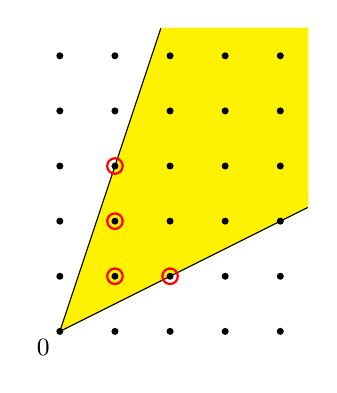
\begin{tikzpicture}[scale=0.7]
	\filldraw[yellow] (0,0) -- (1.833,5.5) -- (4.5,5.5) -- (4.5,2.25) -- cycle;
	\draw (0,0) -- (1.833,5.5);
	\draw (0,0) -- (4.5,2.25) node at (-0.3,-0.3){\small $0$};
	\foreach \x in {0,...,4}
	\foreach \y in {0,...,5}
	{
		\filldraw[fill=black] (\x,\y)  circle (1.5pt);
	}
	\draw[red,thick] (1,1) circle (4pt);
	\draw[red,thick] (1,2) circle (4pt);
	\draw[red,thick] (1,3) circle (4pt);
	\draw[red,thick] (2,1) circle (4pt);
	\end{tikzpicture}
\end{center}

This cone is defined in the input file \verb|2cone.in|:
\begin{Verbatim}
amb_space 2
cone 2
1 3
2 1
\end{Verbatim}
The input tells Normaliz that the ambient space is $\RR^2$, and then a cone with 2 generators is defined, namely the cone $C$ from above.

The figure indicates the Hilbert basis, and this is our first computation goal.

If you prefer to consider the columns of a matrix as input vectors (or have a matrix in this format from another system) you can use the input
\begin{Verbatim}
amb_space 2
cone transpose 2
1 2
3 1
\end{Verbatim}
Note that the number \verb|2| following \verb|transpose| is now the number of \emph{columns}. Later on we will also show the use of formatted matrices.

\subsubsection{The Hilbert basis}
In order to compute the Hilbert basis, we run Normaliz from jNormaliz or by
\begin{Verbatim}
./normaliz -c example/2cone	
\end{Verbatim}
and inspect the output file:
\begin{Verbatim}
4 Hilbert basis elements
2 extreme rays
2 support hyperplanes
\end{Verbatim}
Self explanatory so far.
\begin{Verbatim}
embedding dimension = 2
rank = 2 (maximal)
external index = 1
internal index = 5
original monoid is not integrally closed
\end{Verbatim}
The embedding dimension is the dimension of the space in which the computation is done. The rank is the rank of the lattice $\EE$ (notation as in Section \ref{Term}). In fact, in our example $\EE=\ZZ^2$, and therefore has rank $2$.

For subgroups $G\subset U\subset \ZZ^d$ we denote the order of the torsion subgroup of $U/G$ by the \emph{index} of $G$ in $U$. The \emph{external index} is the index of the lattice $\EE$ in $\ZZ^d$. In our case $\EE=\ZZ^d$, and therefore the external index is $1$. Note: the external index is $1$ exactly when $\EE$ is a direct summand of $\ZZ^d$.

For this example and many others the \emph{original monoid} is well defined: the generators of the cone used as input are contained in $\EE$. (This need not be the case if $\EE$ is a proper sublattice of $\ZZ^d$, and we let the original monoid be undefined in inhomogeneous computations.) Let $G$ be the subgroup generated by the original monoid. The \emph{internal index} is the index of $G$ in $\EE$.

The original monoid is \emph{integrally closed} if and only if the it contains the Hilbert basis, and this is evidently false for our example. We go on.

\begin{Verbatim}
size of triangulation   = 1
resulting sum of |det|s = 5
\end{Verbatim}
The primal algorithm of Normaliz relies on a (partial) triangulation. In our case the triangulation consists of a single simplicial cone, and (the absolute value of) its determinant is~$5$.
\begin{Verbatim}
No implicit grading found
\end{Verbatim}
If you do not define a grading explicitly, Normaliz tries to find one itself: the grading is defined if and only if there is a linear form $\gamma$ on $\EE$ under which all extreme rays of the efficient cone $\CC$ have value $1$, and if so, $\gamma$ is the implicit grading. Such does not exist in our case.

The last information before we come to the vector lists:
\begin{Verbatim}
rank of class group = 0
finite cyclic summands:
5: 1  
\end{Verbatim}
The class group of the monoid $M$ has rank $0$, in other words, it is finite. It has one finite cyclic summand of order $5$.

This is the first instance of a multiset of integers displayed as a sequence of pairs 
\begin{quote}
	\verb|<n>: <m>|
\end{quote} 
Such an entry says: the multiset contains the number \verb|<n>| with multiplicity \verb|<m>.| 


Now we look at the vector lists (typeset in two columns to save space):
\begin{Verbatim}
4 Hilbert basis elements:       2 extreme rays:
1 1                             1 3
1 2                             2 1
1 3
2 1                             2 support hyperplanes:
                                -1  2
                                 3 -1
\end{Verbatim}

The support hyperplanes are given by the linear forms (or inner normal vectors):
\begin{align*}
	-x_1+2x_2&\ge 0,\\
	3x_1-x_2&\ge 0.
\end{align*}

If the order is not fixed for some reason, Normaliz sorts vector lists as follows : (1) by degree if a grading exists and the application makes sense, (2) lexicographically.


\subsubsection{The cone by inequalities}\label{ineq_ex}

Instead by generators, we can define the cone by the inequalities just computed (\verb|2cone_ineq.in|). We use this example to show the input of a formamtted matrix:
\begin{Verbatim}
amb_space auto
inequalities
[[-1  2] [3 -1]]
\end{Verbatim}
A matrix of input type \verb|inequalities| contains \emph{homogeneous} inequalities. Normaliz can determine the dimension of the ambient space from the formatted matrix. Therefore we can declare the ambient space as being ``auto determined'' (but \verb|amb_space 2| is not forbidden).

We get the same result as with \verb|2cone.in| except that the data depending on the original monoid cannot be computed: the internal index and the information on the original monoid are missing since there is no original monoid.

\subsubsection{The interior}\label{strict_ex}
Now we want to compute the lattice points in the interior of our cone. If the cone $C$ is given by the inequalities $\lambda_i(x)\ge0$ (within $\aff(C)$), then the interior is given by the inequalities $\lambda_i(x)>0$. Since we are interested in lattice points, we work with the inequalities $\lambda_i(x)\ge 1$.


The input file \verb|2cone_int.in| says
\begin{Verbatim}
amb_space 2
strict_inequalities 2
-1  2
3 -1
\end{Verbatim}
The strict inequalities encode the conditions
\begin{align*}
	-x_1+2x_2&\ge 1,\\
	3x_1-x_2&\ge 1.
\end{align*}
This is our first example of inhomogeneous input.

Note that the strict inequalities do not define the interior of the cone as a point set. They define a (closed) polyhedron with the same lattice points as the interior.

\begin{center}
	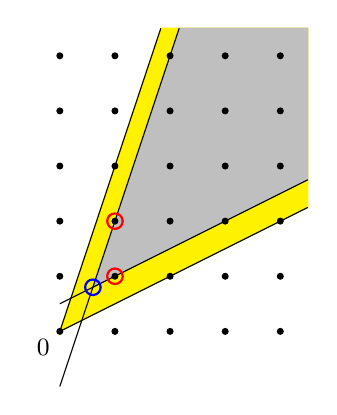
\begin{tikzpicture}[scale=0.7]
	\filldraw[yellow] (0,0) -- (1.833,5.5) -- (4.5,5.5) -- (4.5,2.25) -- cycle;
	\filldraw[lightgray] (0.6,0.8) -- (2.166,5.5) --(4.5,5.5) --  (4.5,2.75) -- cycle;
	\draw (0,0) -- (1.833,5.5);
	\draw (0,0) -- (4.5,2.25) node at (-0.3,-0.3){\small $0$};
	\draw (0,-1) -- (2.166,5.5);
	\draw (0,0.5) -- (4.5,2.75);
	\foreach \x in {0,...,4}
	\foreach \y in {0,...,5}
	{
		\filldraw[fill=black] (\x,\y)  circle (1.5pt);
	}
	\draw[red,thick] (1,1) circle (4pt);
	\draw[red,thick] (1,2) circle (4pt);
	\draw[blue,thick] (0.6,0.8) circle (4pt);
	\end{tikzpicture}
\end{center}
Alternatively we could use the following two equivalent input files, in a more intuitive notation:
\begin{Verbatim}
amb_space 2
constraints 2
-1  2 > 0
3 -1 > 0
\end{Verbatim}
\begin{Verbatim}
amb_space 2
constraints 2
-1  2 >= 1
3 -1 >= 1
\end{Verbatim}
There is an even more intuitive way to type the input file using symbolic constraints that we will introduce in Section \ref{cong_ex}.

Normaliz homogenizes inhomogeneous computations by introducing an auxiliary homogenizing coordinate $x_{d+1}$. The polyhedron is obtained by intersecting the homogenized cone with the hyperplane $x_{d+1}=1$. The recession cone is the intersection with the hyperplane $x_{d+1}=0$. The recession monoid is the monoid of lattice points in the recession cone, and the set of lattice points in the polyhedron is represented by its system of module generators over the recession monoid.

Note that the homogenizing coordinate serves as the denominator for rational vectors. In our example the recession cone is our old friend that we have already computed, and therefore we need not comment on it.

\begin{Verbatim}
2 module generators
4 Hilbert basis elements of recession monoid
1 vertices of polyhedron
2 extreme rays of recession cone
3 support hyperplanes of polyhedron (homogenized)

embedding dimension = 3
affine dimension of the polyhedron = 2 (maximal)
rank of recession monoid = 2
\end{Verbatim}
The only surprise may be the embedding dimension: Normaliz always takes the dimension of the space in which the computation is done. It is the number of components of the output vectors. Because of the homogenization it has increased by $1$.
\begin{Verbatim}
size of triangulation   = 1
resulting sum of |det|s = 25
\end{Verbatim}
In this case the homogenized cone has stayed simplicial, but the determinant has changed.
\begin{Verbatim}
dehomogenization:
0 0 1 
\end{Verbatim}
The dehomogenization is the linear form $\delta$ on the homogenized space that defines the hyperplanes from which we get the polyhedron and the recession cone by the equations $\delta(x)=1$ and $\delta(x)=0$, respectively. It is listed since one can also work with a user defined dehomogenization.
\begin{Verbatim}
module rank = 1
\end{Verbatim}
This is the rank of the module of lattice points in the polyhedron over the recession monoid. In our case the module is an ideal, and so the rank is $1$.

The output of inhomogeneous computations is always given in homogenized form. The last coordinate is the value of the dehomogenization on the listed vectors, $1$ on the module generators, $0$ on the vectors in the recession monoid:
\begin{Verbatim}
2 module generators:          4 Hilbert basis elements of recession monoid:
1 1 1                         1 1 0
1 2 1                         1 2 0
                              1 3 0
                              2 1 0
\end{Verbatim}
The module generators are $(1,1)$ and $(1,2)$.
\begin{Verbatim}
1 vertices of polyhedron:
3 4 5
\end{Verbatim}
Indeed, the polyhedron has a single vertex, namely $(3/5,4/5)$.
\begin{Verbatim}
2 extreme rays of recession cone:     3 support hyperplanes of polyhedron (homogenized):
1 3 0                                 -1  2 -1
2 1 0                                  0  0  1                                
                                       3 -1 -1
\end{Verbatim}
Two support hyperplanes are exactly those that we have used to define the polyhedron -- and it has only $2$. But Normaliz always outputs the support hyperplanes that are needed for the cone that one obtains by homogenizing the polyhedron, as indicated by `homogenized''. The homogenizing variable is always $\ge 0$. In this case the support hyperplane $(0,0,1)$ is essential for the description of the cone. Note that it need not always appear.


\subsection{A lattice polytope}\label{lattice_polytope}\label{polytope_ex}

\begin{minipage}[b]{0.5\textwidth}
The file \ttt{polytope.in} contains

\begin{Verbatim}
amb_space 4
polytope 4
0 0 0
2 0 0
0 3 0
0 0 5
\end{Verbatim}
\end{minipage}
\hspace{1cm}
\begin{minipage}[t]{0.4\textwidth}
\tikzset{facet style/.style={opacity=1.0,very thick,line,join=round}}
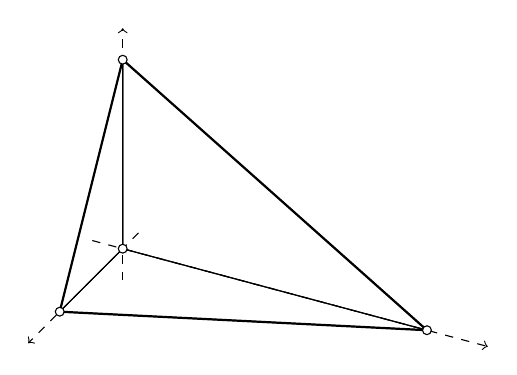
\begin{tikzpicture}[x  = {(-0.5cm,-0.5cm)},
y  = {(0.9659cm,-0.25882cm)},
z  = {(0cm,1cm)},
scale = 0.8]
\draw [->,dashed] (-0.5, 0, 0) -- (3.0,0,0);

\draw [->,dashed] (0, -0.5, 0) -- (0,6.0,0);

\draw [->,dashed] (0, 0, -0.5) -- (0,0,3.5);

\draw[thin] (0,0,0) -- (2,0,0) -- (0,5,0) -- cycle;
\draw[thin] (0,0,0) -- (2,0,0) -- (0,0,3) -- cycle;
\draw[thin] (0,0,0) -- (0,5,0) -- (0,0,3) -- cycle;
\draw[thick] (2,0,0) -- (0,5,0) -- (0,0,3) -- cycle;

\filldraw[fill=white] (0,0,0) circle (2pt);
\filldraw[fill=white] (2,0,0) circle (2pt);
\filldraw[fill=white] (0,5,0) circle (2pt);
\filldraw[fill=white] (0,0,3) circle (2pt);
\end{tikzpicture}
\end{minipage}

This is a good place to mention that Normaliz also accepts matrices (and vectors) in sparse format:

\begin{Verbatim}
amb_space 4
polytope 4 sparse
;
1:2;
2:3;
3:5;
\end{Verbatim}
Each input row, concluded by \verb|;|, lists the indices and the corresponding nonzero values in that row of the matrix.

The Ehrhart monoid of the integral polytope with the $4$
vertices
$$
(0,0,0)\,,\quad (2,0,0)\,,\quad (0,3,0)\quad\text{ and }\quad (0,0,5)
$$
in $\RR^3$ is to be computed. The generators of the Ehrhart monoid are obtained by attaching a further coordinate $1$ to the vertices, and this explains \verb|amb_space 4|. In fact, the input type \verb|polytope| is not only a convenient version of
\begin{Verbatim}
cone 4
0 0 0 1
2 0 0 1
0 3 0 1
0 0 5 1
\end{Verbatim}
It also sets the he grading to be the last coordinate. See \ref{grading} below for general information on gradings.

Running \ttt{normaliz} produces the file \ttt{polytope.out}:
\begin{Verbatim}
19 Hilbert basis elements
18 lattice points in polytope (Hilbert basis elements of degree 1)
4 extreme rays
4 support hyperplanes

embedding dimension = 4
rank = 4 (maximal)
external index = 1
internal index = 30
original monoid is not integrally closed
\end{Verbatim}
Perhaps a surprise: the lattice points of the polytope do not yield all Hilbert basis elements. 
\begin{Verbatim}
size of triangulation   = 1
resulting sum of |det|s = 30
\end{Verbatim}
Nothing really new so far. The grading appears in the output file:
\begin{Verbatim}
grading:
0 0 0 1 

degrees of extreme rays:
1: 4
\end{Verbatim}
Again we encounter the notation \verb|<n>: <m>|: we have $4$ extreme rays, all of degree $1$.
\begin{Verbatim}
Hilbert basis elements are not of degree 1
\end{Verbatim}
Perhaps a surprise: the polytope is not integrally closed as defined in \cite{BG}. Now we see the enumerative data defined by the grading:
\begin{Verbatim}
multiplicity = 30

Hilbert series:
1 14 15 
denominator with 4 factors:
1: 4  

degree of Hilbert Series as rational function = -2

Hilbert polynomial:
1 4 8 5 
with common denominator = 1
\end{Verbatim}
The polytope has $\ZZ^3$-normalized volume $30$ as indicated by the multiplicity (see Section \ref{volume} for a discussion of volumes and multiplicities). The Hilbert (or Ehrhart) function counts the lattice points in $kP$, $k\in\ZZ_+$. The corresponding generating function is a
rational function $H(t)$. For our polytope it is
$$
\frac{1+14t+15t^2}{(1-t)^4}.
$$
The denominator is given in multiset notation: \verb|1: 4| say that the factor $(1-t^1)$ occurs with multiplicity $4$.

The Ehrhart polynomial (again we use a more general term in
the output file) of the polytope is
$$
p(k)=1+4k+8k^2+5k^3\,.
$$
In our case it has integral coefficients, a rare exception. Therefore one usually needs a denominator.

Everything that follows has already been explained.
\begin{Verbatim}

rank of class group = 0
finite cyclic summands:
30: 1  

***********************************************************************

18 lattice points in polytope (Hilbert basis elements of degree 1):
0 0 0 1
...
2 0 0 1

1 further Hilbert basis elements of higher degree:
1 2 4 2

4 extreme rays:                 4 support hyperplanes:
0 0 0 1                         -15 -10 -6 30
0 0 5 1                         0   0  1  0
0 3 0 1                         0   1  0  0
2 0 0 1                         1   0  0  0
\end{Verbatim}

The support hyperplanes give us a description of the polytope
by inequalities: it is the solution of the system of the $4$
inequalities
$$ x_3\ge0\,,\quad
x_2\ge0\,,\quad x_1\ge0\quad\text{ and }\quad
15x_1+10x_2+6x_3\le30\,.
$$

\subsubsection{Only the lattice points}\label{only_lattpoints}

Suppose we want to compute only the lattice points in our polytope. In the language of graded monoids these are the degree $1$ elements, and so we add \verb|Deg1Elements| to our input file (\verb|polytope_deg1.in|):
\begin{Verbatim}
amb_space 4
polytope 4
0 0 0
2 0 0
0 3 0
0 0 5
Deg1Elements
/* This is our first explicit computation goal*/
\end{Verbatim}
We have used this opportunity to include a comment in the input file. The computation of lattice points in a polytope will be taken up again in Sections \ref{project_example} and \ref{LattPoints}.

We lose all information on the Hilbert series, and from the Hilbert basis we only retain the degree $1$ elements.

\subsection{A rational polytope}\label{rational}

The type \verb|polytope| can (now) be used for rational polytopes as well.
\begin{center}
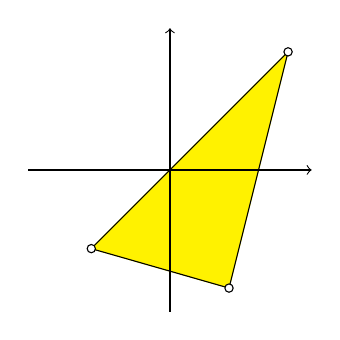
\begin{tikzpicture}[scale=3.0]
\filldraw[yellow] (0.5,0.5) -- (-0.333,-0.333) -- (0.25,-0.5) -- cycle;	
\draw (0.5,0.5) -- (-0.333,-0.333) -- (0.25,-0.5) -- cycle;	
\draw[->] (0,-0.6) --(0,0.6);
\draw[-> ] (-0.6,0) -- (0.6,0);
\filldraw[fill=white] (0.5,0.5) circle (0.5pt);
\filldraw[fill=white] (-0.333,-0.333) circle (0.5pt);
\filldraw[fill=white] (0.25,-0.5) circle (0.5pt);
\end{tikzpicture}
\end{center}

We want to investigate the Ehrhart series of the triangle $P$
with vertices
$$
(1/2,1/2),\ (-1/3,-1/3),\ (1/4,-1/2).
$$
For this example the procedure above yields the input file \ttt{rational.in}:

\begin{Verbatim}
amb_space 3
polytope 3
1/2 1/2
-1/3 -1/3
1/4 -1/2
HilbertSeries
\end{Verbatim}

From the output file we only list the data of the Ehrhart series.
\begin{Verbatim}
multiplicity = 5/8
multiplicity (float) = 0.625

Hilbert series:
1 0 0 3 2 -1 2 2 1 1 1 1 2 
denominator with 3 factors:
1: 1  2: 1  12: 1  

degree of Hilbert Series as rational function = -3

Hilbert series with cyclotomic denominator:
-1 -1 -1 -3 -4 -3 -2 
cyclotomic denominator:
1: 3  2: 2  3: 1  4: 1  

Hilbert quasi-polynomial of period 12:
0:   48 28 15			7:   23 22 15
1:   11 22 15			8:   16 28 15
2:  -20 28 15			9:   27 22 15
3:   39 22 15			10:   -4 28 15
4:   32 28 15			11:    7 22 15
5:   -5 22 15			with common denominator = 48
6:   12 28 15
\end{Verbatim}
The multiplicity is a rational number. Since in dimension $2$
the normalized area (of full-dimensional polytopes) is twice
the Euclidean area, we see that $P$ has Euclidean area $5/16$. If the multiplicity is not integral, we also print it in floating point format, This is certainly superfluous for a fraction like $5/8$, but very handy if the numerator and the denominator have many digits.

Unlike in the case of a lattice polytope, there is no canonical choice of the denominator of the Ehrhart series. Normaliz gives it in $2$ forms. In the first form the numerator polynomial is
$$
1+3t^3+2t^4-t^5+2t^6+2t^7+t^8+t^9+t^{10}+t^{11}+2t^{12}
$$
and the denominator is
$$
(1-t)(1-t^2)(1-t^{12}).
$$
As a rational function, $H(t)$ has degree $-3$. This implies
that $3P$ is the smallest integral multiple of $P$ that
contains a lattice point in its interior.

Normaliz gives also a representation as a quotient of coprime
polynomials with the denominator factored into cyclotomic
polynomials. In this case
we have
$$
H(t)=-\frac{1+t+t^2+t^3+4t^4+3t^5+2t^6}{\zeta_1^3\zeta_2^2\zeta_3\zeta_4}
$$
where $\zeta_i$ is the $i$-th cyclotomic polynomial
($\zeta_1=t-1$, $\zeta_2=t+1$, $\zeta_3=t^2+t+1$,
$\zeta_4=t^2+1$).

Normaliz transforms the representation with cyclotomic
denominator into one with denominator of type
$(1-t^{e_1})\cdots(1-t^{e_r})$, $r=\textup{rank}$, by choosing
$e_r$ as the least common multiple of all the orders of the
cyclotomic polynomials appearing, $e_{r-1}$ as the lcm of those
orders that have multiplicity $\ge 2$ etc.

There are other ways to form a suitable denominator with $3$
factors $1-t^e$, for example
$g(t)=(1-t^2)(1-t^3)(1-t^4)=-\zeta_1^3\zeta_2^2\zeta_3\zeta_4$.
Of course, $g(t)$ is the optimal choice in this case. However,
$P$ is a simplex, and in general such optimal choice may not
exist. We will explain the reason for our standardization
below.

Let $p(k)$ be the number of lattice points in $kP$. Then $p(k)$
is a quasipolynomial:
$$
p(k)=p_0(k)+p_1(k)k+\dots+p_{r-1}(k)k^{r-1},
$$
where the coefficients depend on $k$, but only to the extent
that they are periodic of a certain period $\pi\in\NN$. In our
case $\pi=12$ (the lcm of the orders of the cyclotomic
polynomials).

The table giving the quasipolynomial is to be read as follows:
The first column denotes the residue class $j$ modulo the
period and the corresponding line lists the coefficients
$p_i(j)$ in ascending order of $i$, multiplied by the common
denominator. So
$$
p(k)=1+\frac{7}{12}k+\frac{5}{16}k^2, \qquad k\equiv 0\pod{12},
$$
etc. The leading coefficient is the same for all residue
classes and equals the Euclidean volume (in this case).

Our choice of denominator for the Hilbert series is motivated
by the following fact: $e_i$ is the common period of the
coefficients $p_{r-i},\dots,p_{r-1}$. The user should prove
this fact or at least verify it by several examples.

Especially in the case of a simplex the representation of the Hilbert series shown so far may not be the expected one. In fact, there is a representation in which the exponents of $t$ in the denominator are the degrees of the integral extreme generators. So one would expect the denominator to be $(1-t^2)(1-t^3)(1-t^4)$ in our case. The generalization to the nonsimplicial case uses the degrees of a homogeneous system of parameters (see \cite[p. 200]{BG}). Normaliz can compute such a denominator if the computation goal \verb|HSOP| is set (\verb|rationalHSOP.in|):
\begin{Verbatim}
Hilbert series (HSOP):
1 1 1 3 4 3 2 
denominator with 3 factors:
2: 1  3: 1  4: 1 
\end{Verbatim}

Note that the degrees of the elements in a homogeneous system of parameters are by no means unique and that there is no optimal choice in general. To find a suitable sequence of degrees Normaliz must compute the face lattice of the cone to some extent. Therefore be careful not to ask for \verb|HSOP| if the cone has many support hyperplanes.

\subsubsection{The  series with \ttt{vertices}?}

It is tempting to define the polytope by the input type \verb|vertices|. This choice makes the compuation inhomogeneous, a mode that is mainly meant for (potentially) unbounded polyhedra. But it can be used for polytopes as well, and with this input type you can compute aall of the data that we have seen above. You must ask for the \verb|EhrhartSeries| instead of the \verb|HilbertSeries|. The file \verb|rational_inhom.in| is
\begin{Verbatim}
amb_space 2
vertices 3
1/2 1/2 1
-1/3 -1/3 1
1/4 -1/2 1
EhrhartSeries
\end{Verbatim}

Nevertheless, there is also use for \verb|HilbertSeries| in the inhomogeneous case. But then the grading must be defined on the affine space of the polytope (and not on the cone over the polytope). See Sections \ref{Polytopes} and \ref{count}.

\subsubsection{The rational polytope by inequalities}\label{rat_ineq}

We extract the support hyperplanes of our polytope from the output file and use them as input (\verb|poly_ineq.in|):
\begin{Verbatim}
amb_space 3
inequalities 3
-8  2 3
1 -1 0
2  7 3
grading
unit_vector 3
HilbertSeries
\end{Verbatim}
At this point we have to help Normaliz because it has no way to guess that we want to investigate the polytope defined by the inequalities and the choice $x_3=1$. This is achieved by the specification of the grading that maps every vector to its third coordinate.

This is the first time that we used the shortcut \verb|unit_vector <n>| which represents the $n$th unit vector $e_n\in\RR^d$ and is only allowed for input types which require a single vector.

These data tell us that the polytope, as a subset of $\RR^2$, is defined by the inequalities
\begin{align*}
	-8x_1+2x_2+3&\ge0,\\
	x_1-x_2+0&\ge0,\\
	2x_1+7x_2+3&\ge 0.
\end{align*}
These inequalities are inhomogeneous, but we are using the homogeneous input type \verb|inequalities| which amounts to introducing the grading variable $x_3$ as explained above.


The inequalities as written above look somewhat artificial. It is certainly more natural to write them in the form
\begin{align*}
8x_1-2x_2&\le 3,\\
x_1-x_2&\ge0,\\
2x_1+7x_2&\ge -3.
\end{align*}
and for the direct transformation into Normaliz input we have introduced the type \verb|hom_constraints|. The prefix \verb|hom| indicates that we want homogeneous inequalities whereas plain \verb|constraints|  that we have already seen in Section \ref{strict_ex} give inhomogeneous inequalities. The file \verb|poly_hom_const.in| contains
\begin{Verbatim}
amb_space 3
hom_constraints 3
8 -2 <= 3
1 -1 >= 0
2 7  >= -3
grading
unit_vector 3
HilbertSeries
\end{Verbatim}

You can of course also switch to inhomogeneous input using \verb|inhom_inequalities| or \verb|constrints| in the same way as \verb|polytope| can be replaced by \verb|vertices|.

\subsection{Magic squares}\label{eq_ex}

Suppose that you are interested in the following type of ``square''
\begin{center}
	\begin{tabular}{|l|l|l|}
		\hline
		$x_1$ & $x_2$ & $x_3$\\
		\hline
		$x_4$ & $x_5$ & $x_6$\\
		\hline
		$x_7$ & $x_8$ & $x_9$\\
		\hline
	\end{tabular}
\end{center}
and the problem is to find nonnegative values for $x_1,\dots,x_9$
such that the 3 numbers in all rows, all columns, and both
diagonals sum to the same constant $\mathcal{M}$. Sometimes
such squares are called \emph{magic} and $\mathcal M$ is the
\emph{magic constant}. This leads to a linear system of
equations
\begin{align*}
	& x_1+x_2+x_3=x_4+x_5+x_6;\\
	& x_1+x_2+x_3=x_7+x_8+x_9;\\
	& x_1+x_2+x_3=x_1+x_4+x_7;\\
	& x_1+x_2+x_3=x_2+x_5+x_8;\\
	& x_1+x_2+x_3=x_3+x_6+x_9;\\
	& x_1+x_2+x_3=x_1+x_5+x_9;\\
	& x_1+x_2+x_3=x_3+x_5+x_7.\\
\end{align*}
This system is encoded in the file
\ttt{3x3magic.in}:
\begin{Verbatim}
amb_space 9
equations 7
1 1 1 -1 -1 -1  0  0  0
1 1 1  0  0  0 -1 -1 -1
0 1 1 -1  0  0 -1  0  0
1 0 1  0 -1  0  0 -1  0
1 1 0  0  0 -1  0  0 -1
0 1 1  0 -1  0  0  0 -1
1 1 0  0 -1  0 -1  0  0
grading
sparse 1:1 2:1 3:1;
\end{Verbatim}

The input type \verb|equations| represents \emph{homogeneous} equations. The first equation reads
$$
x_1+x_2+x_3-x_4-x_5-x_6=0,
$$
and the other equations are to be interpreted analogously. The magic constant is a natural choice for the grading. It is given in sparse form, equivalent to the dense form
\begin{Verbatim}
grading
1 1 1 0 0 0 0 0 0
\end{Verbatim}

It seems that we have forgotten to define the cone. This may indeed be the case, but doesn't matter: if there is no input type that defines a cone, Normaliz chooses the positive orthant, and this is exactly what we want in this case.

The output file contains the following:

\begin{Verbatim}
5 Hilbert basis elements
5 lattice points in polytope (Hilbert basis elements of degree 1)
4 extreme rays
4 support hyperplanes

embedding dimension = 9
rank = 3
external index = 1

size of triangulation   = 2
resulting sum of |det|s = 4

grading:
1 1 1 0 0 0 0 0 0 
with denominator = 3
\end{Verbatim}
The input degree is the magic constant. However, as the
denominator $3$ shows, the magic constant is always divisible
by $3$, and therefore the effective degree is $\mathcal M/3$.
This degree is used for the multiplicity, the Hilbert series, and the 
Hilbert basis elements of degree $1$, and other date deopending on the degree.

By introducing the grading denominator, Normaliz has changed the grading defined by you,
and you may not like this. There is a way out: add the option \verb|NoGradingDenom|. We will fdiscuss the consequneces below.
\begin{Verbatim}
degrees of extreme rays:
1: 4  

Hilbert basis elements are of degree 1
\end{Verbatim}
This was not to be expected (and is no longer true for $4\times 4$ squares).
\begin{Verbatim}
multiplicity = 4

Hilbert series:
1 2 1 
denominator with 3 factors:
1: 3  

degree of Hilbert Series as rational function = -1

Hilbert polynomial:
1 2 2 
with common denominator = 1
\end{Verbatim}
The Hilbert series is
$$
\frac{1+2t+t^2}{(1-t)^3}.
$$
The Hilbert polynomial is
$$
P(k)=1+2k+2k^2,
$$
and after substituting $\mathcal M/3$ for $k$ we obtain the
number of magic squares of magic constant $\mathcal M$, provided $3$ divides $\mathcal M$. (If $3\nmid \mathcal M$, there is no magic square of magic constant $\mathcal M$.)
\begin{Verbatim}
rank of class group = 1
finite cyclic summands:
2: 2  
\end{Verbatim}
So the class group is $\ZZ\oplus (\ZZ/2\ZZ)^2$.
\begin{Verbatim}
5 lattice points in polytope (Hilbert basis elements of degree 1):
0 2 1 2 1 0 1 0 2
1 0 2 2 1 0 0 2 1
1 1 1 1 1 1 1 1 1
1 2 0 0 1 2 2 0 1
2 0 1 0 1 2 1 2 0

0 further Hilbert basis elements of higher degree:
\end{Verbatim}
The $5$ elements of the Hilbert basis represent the magic
squares
\begin{center}
	\begin{tabular}{|l|l|l|}
		\hline
		2 & 0 & 1\\
		\hline
		0 & 1 & 2\\
		\hline
		1 & 2 & 0\\
		\hline
	\end{tabular}
	\hspace{10mm}
	\begin{tabular}{|l|l|l|}
		\hline
		1 & 0 & 2\\
		\hline
		2 & 1 & 0\\
		\hline
		0 & 2 & 1\\
		\hline
	\end{tabular}
	\hspace{10mm}
	\begin{tabular}{|l|l|l|}
		\hline
		1 & 1 & 1\\
		\hline
		1 & 1 & 1\\
		\hline
		1 & 1 & 1\\
		\hline
	\end{tabular}
	\hspace{10mm}
	\begin{tabular}{|l|l|l|}
		\hline
		1 & 2 & 0\\
		\hline
		0 & 1 & 2\\
		\hline
		2 & 0 & 1\\
		\hline
	\end{tabular}
	\hspace{10mm}
	\begin{tabular}{|l|l|l|}
		\hline
		0 & 2 & 1\\
		\hline
		2 & 1 & 0\\
		\hline
		1 & 0 & 2\\
		\hline
	\end{tabular}	
\end{center}
All other solutions are linear combinations of these squares
with nonnegative integer coefficients.
One of these $5$ squares is clearly in the interior:
\begin{Verbatim}
4 extreme rays:                  4 support hyperplanes:
0 2 1 2 1 0 1 0 2                -2 -1 0 0  4 0 0 0 0
1 0 2 2 1 0 0 2 1                0 -1 0 0  2 0 0 0 0
1 2 0 0 1 2 2 0 1                0  1 0 0  0 0 0 0 0
2 0 1 0 1 2 1 2 0                2  1 0 0 -2 0 0 0 0
\end{Verbatim}

These $4$ support hyperplanes cut out the cone generated by the magic squares from the linear subspace they generate. Only one is reproduced as a sign inequality. This is due to the fact that the linear subspace has submaximal dimension and there is no unique lifting of linear forms to the full space.
\begin{Verbatim}
6 equations:                 3 basis elements of generated lattice:
1 0 0 0 0  1 -2 -1  1        1 0 -1 -2 0  2  1  0 -1
0 1 0 0 0  1 -2  0  0        0 1 -1 -1 0  1  1 -1  0
0 0 1 0 0  1 -1 -1  0        0 0  3  4 1 -2 -1  2  2
0 0 0 1 0 -1  2  0 -2
0 0 0 0 1 -1  1  0 -1
0 0 0 0 0  3 -4 -1  2
\end{Verbatim}
So one of our equations has turned out to be superfluous (why?). Note that also the equations are not reproduced exactly. Finally, Normaliz lists a basis of the efficient lattice $\EE$  generated by the magic squares. 

Note that the equations and the lattice basis are not uniquely determined. We transform their matrices into reduced row echelon form to force unique output files.

\subsubsection{Blocking the grading denominator}\label{NoGradingDenominator}

As mentioned above, one can block the grading denominator and force Normaliz to use the input grading. For the magic squares we augment the input file as follows (\verb|3x3magicNGD.in|):
\begin{Verbatim}
amb_space 9
equations 7
1 1 1 -1 -1 -1  0  0  0
...
1 1 0  0 -1  0 -1  0  0
grading
sparse 1:1 2:1 3:1;
NoGradingDenom
\end{Verbatim}
The consequences:
\begin{Verbatim}
grading:
1 1 1 0 0 0 0 0 0 

degrees of extreme rays:
3: 4  

multiplicity = 4/9
multiplicity (float) = 0.444444444444

Hilbert series:
1 0 0 2 0 0 1 
denominator with 3 factors:
3: 3  

degree of Hilbert Series as rational function = -3

The numerator of the Hilbert series is symmetric.

Hilbert series with cyclotomic denominator:
-1 0 0 -2 0 0 -1 
cyclotomic denominator:
1: 3  3: 3  

Hilbert quasi-polynomial of period 3:
0:  9 6 2
1:  0 0 0
2:  0 0 0
with common denominator = 9

rank of class group = 1
finite cyclic summands:
2: 2  

***********************************************************************

0 lattice points in polytope (Hilbert basis elements of degree 1):
\end{Verbatim}

It is easy to relate the data with the grading denominator to those without. You must decide yourself what you prefer. One aspect is whether one prefers intrinsic data (with grading denominator) to extrinsic ones that depend on the embedding (without the grading denominator). We will discuss the topic again in Section \ref{Polytopes}.

\subsubsection{With even corners}\label{magiceven}\label{cong_ex}

We change our definition of magic square by requiring that the
entries in the $4$ corners are all even. Then we have to
augment the input file by the following (\ttt{3x3magiceven.in}):
\begin{Verbatim}
congruences 4 sparse
1:1 10:2;
3:1 10:2;
7:1 10:2;
9:1 10:2;
\end{Verbatim}
This sparse form is equivalent to the dense form
\begin{Verbatim}
congruences 4
1 0 0 0 0 0 0 0 0 2
0 0 1 0 0 0 0 0 0 2
0 0 0 0 0 0 1 0 0 2
0 0 0 0 0 0 0 0 1 2
\end{Verbatim}
The first $9$ entries in each row represent the coefficients of the coordinates in the homogeneous congruences, and the last is the modulus:
$$
x_1\equiv 0\mod 2
$$
is the first congruence etc.

We could also define these congruences as symbolic constraints:
\begin{Verbatim}
constraints 4 symbolic
x[1] ~ 0(2);
x[3] ~ 0(2);
x[7] ~ 0(2);
x[9] ~ 0(2);
\end{Verbatim}

The output changes accordingly:


\begin{Verbatim}
9 Hilbert basis elements
0 lattice points in polytope (Hilbert basis elements of degree 1)
4 extreme rays
4 support hyperplanes

embedding dimension = 9
rank = 3
external index = 4

size of triangulation   = 2
resulting sum of |det|s = 8

grading:
1 1 1 0 0 0 0 0 0 
with denominator = 3

degrees of extreme rays:
2: 4  

multiplicity = 1

Hilbert series:
1 -1 3 1 
denominator with 3 factors:
1: 1  2: 2  

degree of Hilbert Series as rational function = -2

Hilbert series with cyclotomic denominator:
-1 1 -3 -1 
cyclotomic denominator:
1: 3  2: 2  

Hilbert quasi-polynomial of period 2:
0:   2 2 1
1:  -1 0 1
with common denominator = 2
\end{Verbatim}
After the extensive discussion in Section \ref{rational} it should be easy for you to write down the Hilbert series and the Hilbert quasipolynomial. (But keep in mind that the grading has a denominator.)
\begin{Verbatim}
rank of class group = 1
finite cyclic summands:
4: 2  

***********************************************************************

0 lattice points in polytope (Hilbert basis elements of degree 1):

9 further Hilbert basis elements of higher degree:
...

4 extreme rays:
0 4 2 4 2 0 2 0 4
2 0 4 4 2 0 0 4 2
2 4 0 0 2 4 4 0 2
4 0 2 0 2 4 2 4 0
\end{Verbatim}
We have listed the extreme rays since they have changed after the introduction of the congruences, although the cone has not changed. The reason is that Normaliz always chooses the extreme rays from the efficient lattice $\EE$.
\begin{Verbatim}
4 support hyperplanes:
...

6 equations:
...                              3 basis elements of generated lattice:
                                   1 0 -1 -2 0  2  1  0 -1
2 congruences:                     0 1 -1 -1 0  1  1 -1  0
1 0 0 0 0 0 0 0 0 2                0 0  3  4 1 -2 -1  2  2
0 1 0 0 1 0 0 0 0 2
\end{Verbatim}
The rank of the lattice has of course not changed, but after the introduction of the congruences the basis has changed.

\subsubsection{The lattice as input}\label{latt_ex}

It is possible to define the lattice by generators. We demonstrate this for the magic squares with even corners. The lattice has just been computed (\verb|3x3magiceven_lat.in|):

\begin{Verbatim}
amb_space 9
lattice 3
 0  1 2 3 1 -1 0  1 2
 2 -1 2 1 1  1 0  3 0
 0  3 0 1 1  1 2 -1 2
grading
1 1 1 0 0 0 0 0 0
\end{Verbatim}
It produces the same output as the version starting from equations and congruences.

\verb|lattice| has a variant that takes the saturation of the sublattice generated by the input vectors (\verb|3x3magic_sat.in|):

\begin{Verbatim}
amb_space 9
saturation 3
 0  1 2 3 1 -1 0  1 2
 2 -1 2 1 1  1 0  3 0
 0  3 0 1 1  1 2 -1 2
grading
1 1 1 0 0 0 0 0 0
\end{Verbatim}
Clearly, we remove the congruences by this choice and arrive at the output of \verb|3x3magic.in|.

\subsection{Decomposition in a numerical semigroup}\label{inhom_eq_ex}

Let $S=\langle 6,10,15\rangle$, the numerical semigroup generated by $6,10,15$. How can $97$ be written as a sum in the generators?\medskip

In other words: we want to find all nonnegative integral solutions to the equation
$$
6x_1+10x_2+15x_3=97.
$$

\begin{minipage}[b]{0.5\textwidth}
Input (\verb|NumSemi.in|):
\begin{Verbatim}
amb_space 3
constraints 1 symbolic
6x[1] + 10x[2] + 15x[3] = 97;
\end{Verbatim}
\end{minipage}
\hspace{1cm}
\begin{minipage}[t]{0.4\textwidth}
\tikzset{facet style/.style={opacity=1.0,very thick,line,join=round}}
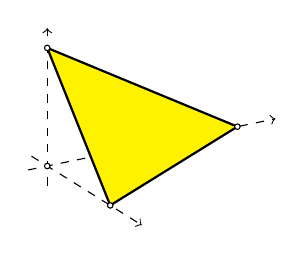
\begin{tikzpicture}[x  = {(0.8cm,-0.5cm)},
y  = {(0.9659cm,0.20cm)},
z  = {(0cm,1cm)},
scale = 0.5]
\draw [->,dashed] (-0.5, 0, 0) -- (3.0,0,0);

\draw [->,dashed] (0, -0.5, 0) -- (0,6.0,0);

\draw [->,dashed] (0, 0, -0.5) -- (0,0,3.5);

%\draw[thin] (0,0,0) -- (2,0,0) -- (0,5,0) -- cycle;
%\draw[thin] (0,0,0) -- (2,0,0) -- (0,0,3) -- cycle;
%\draw[thin] (0,0,0) -- (0,5,0) -- (0,0,3) -- cycle;
\filldraw[color=yellow] (2,0,0) -- (0,5,0) -- (0,0,3) -- cycle;
\draw[thick] (2,0,0) -- (0,5,0) -- (0,0,3) -- cycle;

\filldraw[fill=white] (0,0,0) circle (2pt);
\filldraw[fill=white] (2,0,0) circle (2pt);
\filldraw[fill=white] (0,5,0) circle (2pt);
\filldraw[fill=white] (0,0,3) circle (2pt);
\end{tikzpicture}
\end{minipage}

\medskip
The equation cuts out a triangle from the positive orthant. 

The set of solutions is a module over the monoid $M$ of solutions of the homogeneous equation $6x_1+10x_2+15x_3=0$. So $M=0$ in this case.
\begin{Verbatim}
6 lattice points in polytope (module generators):
2 1 5 1
2 4 3 1
2 7 1 1
7 1 3 1
7 4 1 1
12 1 1 1

0 Hilbert basis elements of recession monoid:
\end{Verbatim}
The last line is as expected, and the $6$ lattice popints (or module generators) are the goal of the computation.

Normaliz is smart enough to recognize that it must compute the lattice points in a polygon, and does exactly this. You can recognize it in the console output:  Normaliz \version\ has used the project-and-lift algorithm. We will discuss it further in Section \ref{project_example} and Section \ref{project}.

 For those who like to play: add the option \verb|--NoProjection| to the command line. Then the terminal output will change; Normaliz computes the lattice points as a truncated Hilbert basis via a triangulation (only one simplicial cone in this case).

\subsection{A job for the dual algorithm}\label{job_dual}

We increase the size of the magic squares to $5\times 5$. Normaliz can do the same computation as for $3\times 3$ squares, but this will take some minutes. Suppose we are only interested in the Hilbert basis, we should use the dual algorithm for this example. (The dual algorithm goes back to Pottier \cite{Po}.) The input file is \ttt{5x5dual.in}:

\begin{Verbatim}
amb_space 25
equations 11
1 1 1 1 1 -1 -1 -1 -1 -1  0  0  0  0  0  0  0  0  0  0  0  0  0  0  0
...
1 1 1 1 0  0  0  0 -1  0  0  0 -1  0  0  0 -1  0  0  0 -1  0  0  0  0
grading
1 1 1 1 1 0 0 0 0 0 0 0 0 0 0 0 0 0 0 0 0 0 0 0 0
HilbertBasis
\end{Verbatim}
The input file does not say anything about the dual algorithm mentioned in the section title. With this input it is chosen automatically. See Section \ref{div_labor} for a discussion of when this happens. But you can insist on the dual algorithm by adding \verb|DualMode| to the input (or \verb|-d| to the command line). Or, if you want to compare it to the primal algorithm add \verb|PrimalMode| (or \verb|-P| to the command line).


The Hilbert basis contains $4828$ elements, too many to be listed here.

With the file \verb|5x5.in| you can compute the Hilbert basis and the Hilbert series, and the latter with HSOP:
\begin{Verbatim}
Hilbert series (HSOP):
1 15 356 4692 36324 198467 ... 198467 36324 4692 356 15 1 
denominator with 15 factors:
1: 5  2: 3  6: 2  12: 1  60: 2  420: 1  1260: 1  

degree of Hilbert Series as rational function = -5

The numerator of the Hilbert Series is symmetric.
\end{Verbatim}
In view of the length of the numerator of the Hilbert series it may be difficult to observe the symmetry. So Normaliz does it for you.  The symmetry shows that the monoid is Gorenstein, but if you are only interested in the Gorenstein property, there is a much faster way to check it (see Section \ref{Gorenstein}).

The size $6\times 6$ is out of reach for the Hilbert series, but the Hilbert basis can be computed (in the automatically chosen dual mode). It takes some hours.

\subsection{A dull polyhedron}\label{inhom_ineq_ex}

We want to compute the polyhedron defined by the inequalities
\begin{align*}
	\xi_2 &\ge -1/2,\\
	\xi_2 &\le 3/2,\\
	\xi_2 &\le \xi_1+3/2.
\end{align*}
They are contained in the input file \verb|InhomIneq.in|:
\begin{Verbatim}
amb_space 2
constraints 3
 0 1 >= -1/2
 0 1 <=  3/2
-1 1 <=  3/2
grading
unit_vector 1
FVector
\end{Verbatim}
The grading says that we want to count points by the first coordinate, namely along the green lines:
\begin{center}
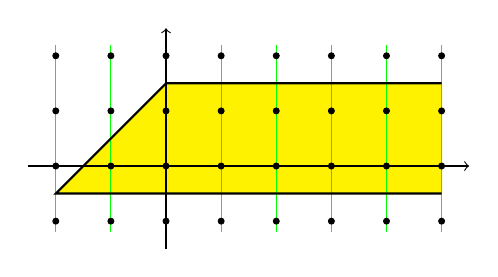
\begin{tikzpicture}[scale=0.7]
	
	\filldraw[yellow] (5,-0.5) -- (-2,-0.5) -- (0,1.5) -- (5,1.5) -- cycle;
	
	\foreach \x in {-2,...,5}
	{
		\draw[color=green] (\x,-1.2) -- (\x,2.2);
	} 
	
	\foreach \x in {-2,...,5}
	\foreach \y in {-1,...,2}
	{
		\filldraw[fill=black] (\x,\y)  circle (1.5pt);
	}
	\draw[->] (-2.5,0) -- (5.5,0);
	\draw[->] (0,-1.5) -- (0,2.5);
	\draw[thick] (5,-0.5) -- (-2,-0.5) -- (0,1.5) -- (5,1.5);

\end{tikzpicture}
\end{center}

It yields the output
\begin{Verbatim}
2 module generators
1 Hilbert basis elements of recession monoid
2 vertices of polyhedron
1 extreme rays of recession cone
3 support hyperplanes of polyhedron (homogenized)

f-vector:
1 2 3 1 
\end{Verbatim}
The empty set is the intersection of all facets, and this gives the first entry $1$. Then we have $2$ vertices, $3$ edges, and finally the full polyhedron.

The out put continues:

\begin{Verbatim}
embedding dimension = 3
affine dimension of the polyhedron = 2 (maximal)
rank of recession monoid = 1

size of triangulation   = 1
resulting sum of |det|s = 8

dehomogenization:
0 0 1 

grading:
1 0 0 
\end{Verbatim}
The interpretation of the grading requires some care in the inhomogeneous case. We have extended the input grading vector by an entry $0$ to match the embedding dimension. For the computation of the degrees of \emph{lattice points} in the ambient space you can either use only the first $2$ coordinates or take the full scalar product of the point in homogenized coordinates and the extended grading vector.

\begin{Verbatim}
module rank = 2
multiplicity = 2
\end{Verbatim}
The module rank is $2$ in this case since we have two ``layers'' in the solution module that are parallel to the recession monoid. This is of course also reflected in the Hilbert series.
\begin{Verbatim}
Hilbert series:
1 1 
denominator with 1 factors:
1: 1  

shift = -1
\end{Verbatim}
We haven't seen a shift yet. It is always printed (necessarily) if the Hilbert series does not start in degree $0$. In our case it starts in degree $-1$ as indicated by the shift $-1$. We thus get the Hilbert series
$$
t^{-1}\,\frac{t+t}{1-t}=\frac{t^{-1}+1}{1-t}.
$$

Note: We used the opposite convention for the shift in Normaliz 2.

Note that the Hilbert (quasi)polynomial is always computed for the unshifted monoid defined by the input data. (This was different in previous versions of Normaliz.) 
\begin{Verbatim}
degree of Hilbert Series as rational function = -1

Hilbert polynomial:
2 
with common denominator = 1

***********************************************************************

2 module generators:
-1 0 1
0 1 1

1 Hilbert basis elements of recession monoid:
1 0 0

2 vertices of polyhedron:
-4 -1 2
0  3 2

1 extreme rays of recession cone:
1 0 0

3 support hyperplanes of polyhedron (homogenized):
0 -2 3
0  2 1
2 -2 3
\end{Verbatim}

The dual algorithm that was used in Section \ref{job_dual} can also be applied to inhomogeneous computations. We would of course loose the Hilbert series. In certain cases it may be preferable to suppress the computation of the vertices of the polyhedron if you are only interested in the integer points; see Section \ref{InhomDual}.

\subsubsection{Defining it by generators}\label{polyh_ex}

If the polyhedron is given by its vertices and the recession cone, we can define it by these data (\verb|InhomIneq_gen.in|):
\begin{Verbatim}
amb_space 2
vertices 2
-4 -1 2
0  3 2
cone 1
1 0
grading
unit_vector 1
\end{Verbatim}
The output is identical to the version starting from the inequalities.

\subsection{The Condorcet paradox}\label{Condorcet}

In social choice elections each of the $k$ voters picks a linear preference order of the $n$ candidates. There are $n!$ such orders. The election result is the vector $(x_1,\dots,x_N), $N=n!, in which $x_i$ is the number of voters that have chosen the $i$-th preference order in, say, lexicographic enumeration of these orders. In the following we assume the \emph{impartial anonymous culture} according to which every preference order has the same basic weight of $1/n!$. 
\medskip 

We say that candidate $A$ \emph{beats} candidate $B$ if the majority of the voters prefers $A$ to $B$. As the Marquis de \emph{Condorcet} (and others) observed, ``beats'' is not transitive, and an election may exhibit the \emph{Condorcet paradox}: there is no Condorcet winner. (See \cite{BS} and the references given there for more information.)

We want to find the probability for $k\to\infty$ that there is a Condorcet winner for $n=4$ candidates. The event that $A$ is the Condorcet winner can be expressed by linear inequalities on the election outcome (a point in $24$-space). The wanted probability is the lattice normalized volume of the polytope cut out by the inequalities at $k=1$. The file \verb|Condorcet.in|:

\begin{Verbatim}
amb_space 24
inequalities 3
1 1 1 1 1 1 -1 -1 -1 -1 -1 -1   1  1 -1 -1  1 -1   1  1 -1 -1  1 -1
1 1 1 1 1 1  1  1 -1 -1  1 -1  -1 -1 -1 -1 -1 -1   1  1  1 -1 -1 -1
1 1 1 1 1 1  1  1  1 -1 -1 -1   1  1  1 -1 -1 -1  -1 -1 -1 -1 -1 -1
nonnegative
total_degree
Multiplicity
\end{Verbatim}
The first inequality expresses that $A$ beats $B$, the second and the third say that $A$ beats $C$ and $D$. (So far we do not exclude ties, and they need not be excluded for probabilities as $k\to\infty$.)

In addition to these inequalities we must restrict all variables to nonnegative values, and this is achieved by adding the attribute \verb|nonnegative|. The grading is set by \verb|total_degree|. It replaces the grading vector with $24$ entries $1$. Finally \verb|Multiplicity| sets the computation goal.

From the output file we only mention the quantity we are out for:
\begin{Verbatim}
multiplicity = 1717/8192
multiplicity (float) = 0.209594726562
\end{Verbatim}
Since there are $4$ candidates, the probability for the existence of a Condorcet winner is $1717/2048=0.209595$.

We can refine the information on the Condorcet paradox by computing the Hilbert series. Either we delete \verb|Multiplicity| from the input file or, better, we add \verb|--HilbertSeries| (or simply \verb|-q|) on the command line. The result:
\begin{Verbatim}
Hilbert series:
1 5 133 363 4581 8655 69821 100915 ... 12346 890 481 15 6 
denominator with 24 factors:
1: 1  2: 14  4: 9

degree of Hilbert Series as rational function = -25
\end{Verbatim}

If your executable of Normaliz was built with CoCoALib (ee Section \ref{Compile}), for example the executablse for Linux or Mac OS from our distribution or in the Docker image, it uses symmetrization for the computation of the Hilbert series. If not, then simply disregard any remark on symmetrization. Everything runs very quickly also without it.

If symmetrization has been used, you will also find a file \verb|Condorcet.symm.out| in your directory. It contains the data computed for the symmetrization. You need not care at this point. We take continue the discussion of symmetrization in Section \ref{symmetrize}.

\subsubsection{Excluding ties}\label{excluded_ex}

Now we are more ambitious and want to compute the Hilbert series for the Condorcet paradox, or more precisely, the number of election outcomes having $A$ as the Condorcet winner depending on the number $k$ of voters. Moreover, as it is customary in social choice theory, we want to exclude ties. The input file changes to \verb|CondorcetSemi.in|:
\begin{Verbatim}
amb_space 24
excluded_faces 3
1 1 1 1 1 1 -1 -1 -1 -1 -1 -1   1  1 -1 -1  1 -1   1  1 -1 -1  1 -1
1 1 1 1 1 1  1  1 -1 -1  1 -1  -1 -1 -1 -1 -1 -1   1  1  1 -1 -1 -1
1 1 1 1 1 1  1  1  1 -1 -1 -1   1  1  1 -1 -1 -1  -1 -1 -1 -1 -1 -1
nonnegative
total_degree
HilbertSeries
\end{Verbatim}
We could omit \verb|HilbertSeries|, and the computation would include the Hilbert basis. The type \verb|excluded_faces| only affects the Hilbert series. In every other respect it is equivalent to \verb|inequalities|.

From the file \verb|CondorcetSemi.out| we only display the Hilbert series:
\begin{Verbatim}
Hilbert series:
6 15 481 890 12346 ... 100915 69821 8655 4581 363 133 5 1 
denominator with 24 factors:
1: 1  2: 14  4: 9  

shift = 1

degree of Hilbert Series as rational function = -24
\end{Verbatim}
Surprisingly, this looks like the Hilbert series in the previous section read backwards, roughly speaking. This is true, and one can explain it as we will see below. 

It is justified to ask why we don't use \verb|strict_inequalities| instead of \verb|excluded_faces|. It does of course give the same Hilbert series. However, Normaliz cannot (yet) apply symmetrization in inhomogeneous computations. Moreover, the algorithmic approach is different, and according to our experience \verb|excluded_faces| is more efficient, independently of symmetrization. 

\subsubsection{At least one vote for every preference order}\label{strict_signs_ex}

Suppose we are only interested in elections in which every preference order is chosen by at least one voter. This can be modeled as follows (\verb|Condorcet_one.in|):
\begin{Verbatim}
amb_space 24
inequalities 3
1 1 1 1 1 1 -1 -1 -1 -1 -1 -1   1  1 -1 -1  1 -1   1  1 -1 -1  1 -1
1 1 1 1 1 1  1  1 -1 -1  1 -1  -1 -1 -1 -1 -1 -1   1  1  1 -1 -1 -1
1 1 1 1 1 1  1  1  1 -1 -1 -1   1  1  1 -1 -1 -1  -1 -1 -1 -1 -1 -1
strict_signs
1 1 1 1 1 1 1 1 1 1 1 1 1 1 1 1 1 1 1 1 1 1 1 1
total_degree
HilbertSeries
\end{Verbatim}
The entry $1$ at position $i$ of the vector \verb|strict_signs| imposes the inequality $x_i\ge1$. A $-1$ would impose the inequality $x_i\le -1$, and the entry $0$ imposes no condition on the $i$-th coordinate.

\begin{Verbatim}
Hilbert series:
1 5 133 363 4581 8655 69821 100915 ... 12346 890 481 15 6 
denominator with 24 factors:
1: 1  2: 14  4: 9  

shift = 24

degree of Hilbert Series as rational function = -1
\end{Verbatim}
Again we encounter (almost) the Hilbert series of the Condorcet paradox (without side conditions). It is time to explain this coincidence. Let $C$ be the Condorcet cone defined by the nonstrict inequalities, $M$ the monoid of lattice points in it, $I_1\subset M$ the ideal of lattice points avoiding the $3$ facets defined by ties, $I_2$ the ideal of lattice points with strictly positive coordinates, and finally $I_3$ the ideal of lattice points in the interior of $C$. Moreover, let $\mathds{1}\in\ZZ^{24}$ be the vector with all entries $1$. 

Since $\mathds{1}$ lies in the three facets defining the ties, it follows that $I_2=M+\mathds{1}$. This explains why we obtain the Hilbert series of $I_2$ by multiplying the Hilbert series of $M$ by $t^{24}$, as just observed. Generalized Ehrhart reciprocity (see \cite[Theorem 6.70]{BG}) then explains the Hilbert series of $I_1$ that we observed in the previous section. Finally, the Hilbert series of $I_3$ that we don't have displayed is obtained from that of $M$ by  ``ordinary'' Ehrhart reciprocity. But we can also obtain $I_1$ from $I_3$: $I_1=I_3-\mathds{1}$, and generalized reciprocity follows from ordinary reciprocity in this very special case. (Also see \cite{BIS2}.)

The essential point in these arguments (apart from reciprocity) is that $\mathds{1}$ lies in all support hyperplanes of $C$ except the coordinate hyperplanes.

You can easily compute the Hilbert series of $I_3$ by making all inequalities strict.

As the terminal output shows, symmetrization has not been applied for the reason mentioned above: \verb|strict_signs| is an inhomogeneous input type. It would of course be possible to encode the strict signs as \verb|excluded_faces|. Then the sparse format of matrices is very handy:
\begin{Verbatim}
excluded_faces 24
1:1;
1:2;
...
1:24;
\end{Verbatim}
This is a shorthand for the unit matrix.

\subsubsection{The f-vector with codimension bound}\label{codim_bound}

Suppose we are interested in the f-vector of the cone defined by \ttt{Condorcet.in}. In view of the rather high dimension the face lattice must be expwected to be extremely large, but computing the f-vector  to codimension $4$ should be no problem. Indeed it is not. We use \ttt{CondorcetFV.in}:
\begin{Verbatim}
...
FVector
face_codim_bound 4
\end{Verbatim}

Then we find in the output file:
\begin{Verbatim}
f-vector (possibly truncated):
17550 2925 351 27 1
\end{Verbatim}
Note that the face numbers are listed by descending codimension or, equivalently, by increasing dimension. The leftmost number is the number of faces in the highest codimenion that has been computed. So we have $17550$ codimension $4$ faces.


\subsection{Testing normality}\label{normalization_ex}

We want to test the monoid $A_{4\times 4\times 3}$ defined by $4\times4\times3$ contingency tables for normality (see \cite{BHIKS} for the background). The input file is \ttt{A443.in}:
\begin{Verbatim}
amb_space 40
cone_and_lattice 48
1 0 0 0 0 0 0 0 0 0 0 0 0 0 0 0 1 0 0 0 0 0 0 0 0 0 0 0 1 0 0 0 0 0 0 0 0 0 0 0
...
0 0 0 0 0 0 0 0 0 0 0 0 0 0 0 1 0 0 0 0 0 0 0 0 0 0 0 1 0 0 0 0 0 0 0 0 0 0 0 1
HilbertBasis
\end{Verbatim}
Why \verb|cone_and_lattice|? Well, we want to find out whether the monoid is normal, i.e., whether $M=C(M)\cap\gp(M)$. If $M$ is even integrally closed in $\ZZ^{24}$, then it is certainly integrally closed  in the evidently smaller lattice $\gp(M)$, but the converse does not hold in general, and therefore we work with the lattice generated by the monoid generators.

It turns out that the monoid is indeed normal:
\begin{Verbatim}
original monoid is integrally closed
\end{Verbatim}
Actually the output file reveals that $M$ is even integrally closed in $\ZZ^{24}$: the external index is $1$, and therefore $\gp(M)$ is integrally closed in $\ZZ^{24} $. 

The output files also shows that there is a grading on $\ZZ^{24}$ under which all our generators have degree $1$. We could have seen this ourselves: Every generator has exactly one entry $1$ in the first $16$ coordinates. (This is clear from the construction of $M$.)

A noteworthy detail from the output file:
\begin{Verbatim}
size of partial triangulation   = 48
\end{Verbatim}
It shows that Normaliz uses only a partial triangulation in Hilbert basis computations; see \cite{BHIKS}.

It is no problem to compute the Hilbert series as well if you are interested in it. Simply add \verb|-q| to the command line or remove \verb|HilbertBasis| from the input file. Then a full triangulation is needed (size $2,654,272$).

Similar examples are \verb|A543|, \verb|A553| and \verb|A643|. The latter is not normal, as we will see below. Even on a standard PC or laptop, the Hilbert basis computation does not take very long because Normaliz uses only a partial triangulation. The Hilbert series can still be determined, but the computation time will grow considerably since the it requires a full triangulation. See \cite{BIS} for timings.

\subsubsection{Computing just a witness}\label{IsIC}

If the Hilbert basis is large and there are many support hyperplanes, memory can become an issue for Normaliz, as well as computation time. Often one is only interested in deciding whether the given monoid is integrally closed (or normal). In the negative case it is enough to find a single element that is not in the original monoid -- a witness disproving integral closedness. As soon as such a witness is found, Normaliz stops the Hilbert basis computation (but will continue to compute other data if they are asked for). We look at the example \verb|A643.in| (for which the full Hilbert basis is not really a problem):


\begin{Verbatim}
amb_space 54
cone_and_lattice 72
1 0 0 0 0 0 0 0 0 0 0 0 0 0 0 0 0 0 0 0 0 0 0 0 1 0 ...
...
0 0 0 0 0 0 0 0 0 0 0 0 0 0 0 0 0 0 0 0 0 0 0 1 0 0 ...
IsIntegrallyClosed
\end{Verbatim}
Don't add \verb|HilbertBasis| because it will overrule \verb|IsIntegrallyClosed|!

The output:
\begin{Verbatim}
72 extreme rays
153858 support hyperplanes

embedding dimension = 54
rank = 42
external index = 1
internal index = 1
original monoid is not integrally closed
witness for not being integrally closed:
0 0 1 0 1 1 1 1 0 0 1 0 0 1 0 1 0 1 1 0 1 1 0 0 1 1 1 0 0 1 1 0 0 1 1 ...

grading:
1 1 1 1 1 1 1 1 1 1 1 1 1 1 1 1 1 1 1 1 1 1 1 1 0 0 0 0 0 0 0 0 0 0 0 ...

degrees of extreme rays:
1: 72  

***********************************************************************

72 extreme rays:
0 0 0 0 0 0 0 0 0 0 0 0 0 0 0 0 0 0 0 0 0 0 0 1 0 0 0 0 0 0 0 0 0 0 0 0 ...
...
\end{Verbatim}

If you repeat such a computation, you may very well get a different witness if several parallel threads find witnesses. Only one of them is delivered.

\subsection{Convex hull computation/vertex enumeration}

Normaliz computes convex hulls as should be very clear by now, and the only purpose of this section is to emphasize that Normaliz can be restricted to this task by setting an explicit computation goal. By convex hull computation we mean the determination of the support hyperplanes of a polyhedron is given by generators (or vertices). The converse operation is vertex enumeration. Both amount to the dualization of a cone, and can therefore be done by the same algorithm.

As an example we take the input file \verb|cyclicpolytope30-15.in|, the cyclic polytope of dimension 15 with 30 vertices (suggested by D. Avis and Ch. Jordan):
\begin{Verbatim}
/* cyclic polytope of dimension 15 with 30 vertices */
amb_space 16
polytope 30
1 1 1 1 1 1 1 1 1 1 1 1 1 1 1
2 4 8 16 32 64 128 256 512 1024 2048 4096 8192 16384 32768
...
30 900 27000 810000 ... 478296900000000000000 14348907000000000000000
SupportHyperplanes
\end{Verbatim}
Already the entries of the vertices show that the computation cannot be done in 64 bit arithmetic. But you need not be worried. Just start Normaliz as usual. It will simply switch to infinite precision by itself, as shown by the terminal output (use the option \verb|-c| or \verb|--Verbose|).
\begin{Verbatim}
                                                    \.....|
                    Normaliz 3.2.0                   \....|
                                                      \...|
     (C) The Normaliz Team, University of Osnabrueck   \..|
                    January  2017                       \.|
                                                         \|
************************************************************
Compute: SupportHyperplanes 
Could not convert 15181127029874798299.
Arithmetic Overflow detected, try a bigger integer type!
Restarting with a bigger type.
************************************************************
starting primal algorithm (only support hyperplanes) ...
Generators sorted lexicographically
Start simplex 1 2 3 4 5 6 7 8 9 10 11 12 13 14 15 16 
gen=17, 72 hyp
gen=18, 240 hyp
gen=19, 660 hyp
gen=20, 1584 hyp
gen=21, 3432 hyp
gen=22, 6864 hyp
gen=23, 12870 hyp
gen=24, 22880 hyp
gen=25, 38896 hyp
gen=26, 63648 hyp
gen=27, 100776 hyp
gen=28, 155040 hyp
gen=29, 232560 hyp
gen=30, 341088 hyp
Pointed since graded
Select extreme rays via comparison ... done.
------------------------------------------------------------
transforming data... done.
\end{Verbatim}
Have a look at the output file if you are not afraid of $341088$ linear forms.

If you have looked closely at the terminal output above, you should have stumbled on the lines
\begin{Verbatim}
Could not convert 15181127029874798299.
Arithmetic Overflow detected, try a bigger integer type!
\end{Verbatim}
They show that Normaliz has tried the computation in 64 bit integers, but encountered a number that is too large for this precision. It has automatically switched to infinite precision. (See Section \ref{Integer} for more information on integer types.)

\subsection{Lattice points in a polytope and its Euclidean volume}\label{project_example}

The computation of lattice points in a polytope can be viewed as a truncated Hilbert basis computation, and we have seen in preceding examples. But Normaliz can be restricted to their computation, with homogeneous as well as with inhomogeneous input. Let us look at \verb|ChF_8_1024.in|:

\begin{Verbatim}
amb_space 8
constraints 16
0.10976576 0.2153132834 ... 0.04282847494 >= -1/2
...
0.10976576 -0.2153132834 ... -0.04282847494 >= -1/2
0.10976576 0.2153132834 ... 0.04282847494 <= 1/2
0.10976576 -0.2153132834 ...-0.04282847494 <= 1/2
LatticePoints
ProjectionFloat
\end{Verbatim}

This example comes from numerical analysis; see Ch. Kacwin, J. Oettershagen and T. Ullrich, On the orthogonality of the Chebyshev-Frolov lattice and applications, Monatsh. Math. 184 (2017), 425--441). Its origin explains the decimal fractions in the input. Normaliz converts them immediately into ordinary fractions of type numerator/denominator, and then makes the input integral as usual.

In the output file you can see to what integer vectors Normaliz has converted the inequalities of the input file:
\begin{Verbatim}
16 support hyperplanes of polyhedron (homogenized):
  5488288000  10765664170  ...  2141423747 25000000000
  ...
 -5488288000  10765664170 ...   2141423747 25000000000
\end{Verbatim}

The option \verb|ProjectionFloat| indicates that we want to compute the lattice points in the polytope defined by the inequalities and that we want to use the floating point variant of the project-and-lift algorithm; \verb|Projection| would make Normaliz use its ordinary arithmetic in this algorithm. For our example the difference in time is not really significant, but when you try \verb|VdM_16_1048576.in|, it becomes very noticeable. Let us have a look at the relevant part of then terminal output:
\begin{Verbatim}
Polyhedron is parallelotope
Computing lattice points by project-and-lift
LLL based on support hyperplanes
Projection
embdim 9 inequalities 16
...
embdim 6 inequalities 140
...
embdim 2 inequalities 2
embdim 1 inequalities 0
Lifting
Lifting to dimension 2
Lifting to dimension 3
...
Lifting to dimension 8
Lifting to dimension 9
embdim 2 LatticePoints 5
embdim 3 LatticePoints 21
...
embdim 8 LatticePoints 907
embdim 9 LatticePoints 1067
Project-and-lift complete
\end{Verbatim}

We start with embedding dimension $9$ since we need a homogenizing coordinate in inhomogeneous computations. Then the polytope is successively projected onto a coordinate hyperplane until we reach a line segment given by $2$ inequalities. In the second part Normaliz lifts the lattice points back through all projections. The following figure illustrates the procedure for a polygon that is projected to a line segment.
\begin{center}
	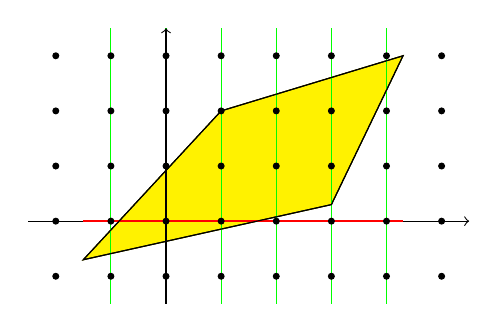
\begin{tikzpicture}[scale=0.7]
	
	\filldraw[yellow] (-1.5,-0.7) -- (1,2) -- (4.3,3) -- (3,0.3) -- cycle;
	\draw (-1.5,-0.7) -- (1,2) -- (4.3,3) -- (3,0.3) -- cycle;
	
	\foreach \x in {-1,...,4}
	{
		\draw[green] (\x,-1.5) -- (\x,3.5);
	}
	\draw[->] (-2.5,0) -- (5.5,0);
	\draw[->] (0,-1.5) -- (0,3.5);
	%\draw (-1.5,-1.5) -- (-1.5,3.5);
	\draw[color=red,thick] (-1.5,0) -- (4.3,0);
	
	\foreach \x in {-2,...,5}
	\foreach \y in {-1,...,3}
	{
		\filldraw[fill=black] (\x,\y)  circle (1.5pt);
	}
	\draw (-1.5,-0.7) -- (1,2) -- (4.3,3) -- (3,0.3) -- cycle;
	%\draw[thick] (5,0) -- (-1,-0) -- (0,1) -- (5,1);
	\end{tikzpicture}
\end{center}
The green lines show the fibers over the lattice points in the (red) line segment. Note that not every lattice point in the projection must be liftable to a lattice point in the next higher dimension.

In \verb|ChF_8_1024.out| we see
\begin{Verbatim}
1067 lattice points in polytope (module generators):
-4  0  0  0  0  0  0  0 1
-3  0  0  0 -1  0  0  0 1
-3  0  0  0  0  0  0  0 1
...
3  0  0  0  0  0  0  0 1
3  0  0  0  1  0  0  0 1
4  0  0  0  0  0  0  0 1
\end{Verbatim}

Normaliz finds out that our polytope is in fact a parallelotope. This allows Normaliz to suppress the computation of its vertices. We are not interested in them, and they look frightening when written as ordinary fractions (computed with the additional option \verb|SupportHyperplanes|). This is only the first vertex, the denominator is the number in the last row:
\begin{Verbatim}
256 vertices of polyhedron:
-7831972155307708173239167258085974255845869779051329651906336771582421875
-2560494334732147696394408175864650673712115229853232268085759500000000000
2411932924117448250036041241683237083742860005142447171295674845000000000
-2170682283899852950367663781367299946065844697990214478942400250000000000
1846013540077621750562232333569651551559659207659438074760922800500000000
-1450403531662801634587765586956338287943865886737024582718631750000000000
999055328718773316303519268629091038893656784654239444024061220000000000
-509313990522468215816366827427428831508901797188810249435062450000000000
2292486335803169657316823615602461625422283571089603408672092012129842506
...
\end{Verbatim}

Not all polytopes are parallelotopes, and in most cases Normaliz must compute the vertices or extreme rays as an auxiliary step, even if we are not interested in them. You can always add the option
\begin{itemize}
\itemtt [NoExtRaysOutput]
\end{itemize}
if you want to suppress their output. (The numerical information on the number of extreme rays etc. will however be included in the output file if it is available.) Similarly one can suppress the output of support hyperplanes by
\begin{itemize}
	\itemtt [NoSuppHypsOutput]
\end{itemize}

On the other hand, the information provided by the vertices or support hyperplanes may be important. Instead of the unreadable integer output shown above, you can ask for
\begin{itemize}
	\itemtt [VerticesFloat]
\end{itemize}
Then the vertices of polyhedra are printed in floating point format:
\begin{Verbatim}
256 vertices of polyhedron:
-3.41637   -1.11691     1.0521  ... 0.435796  -0.222167          1 
-3.41637  -0.946868   0.435796  ...  -1.0521   0.632677          1
...
\end{Verbatim}
Notre that they can only be printed if a polyhedron is defined. This is always the case in inhomogeneous computations, but in the homogeneous case a grading is necessary.

Similarly we can get the support hyperplanes in floating point format (they are only defined up to a positive scalar multiple) by
\begin{itemize}
	\itemtt [SuppHypsFloat]
\end{itemize}
resulting in
\begin{Verbatim}
16 support hyperplanes of polyhedron (homogenized):
-0.219532  -0.430627  -0.405641  ...  -0.168022 -0.0856569          1 
-0.219532  -0.365068  -0.168022  ...   0.405641    0.24393          1 
...  
\end{Verbatim}

By its construction, our polytope should have Euclidean volume $1024$. We can confirm this number by computing the volume, using the option
\begin{itemize}
	\itemtt [Volume, -V]
\end{itemize}
We get
\begin{Verbatim}
volume (normalized) = 205078125000...00/49670537275735342575...58763
volume (normalized, float) =41287680.0308
volume (Euclidean) = 1024.00000076
\end{Verbatim}
The result makes us happy, despite of the small inaccuracy of the floating point computation on which the Euclidean volume is based. See Section \ref{volume} for a discussion of volumes and multiplicities.

\subsection{The integer hull}\label{IntHull}

The integer hull of a polyhedron $P$ is the convex hull of the set of lattice points in $P$ (despite of its name, it usually does not contain $P$). Normaliz computes by first finding the lattice points and then computing the convex hull. The computation of the integer hull is requested by the computation goal \verb|IntegerHull|.

The computation is somewhat special since it creates a second cone (and lattice) $C_\textup{int}$. In homogeneous computations the degree $1$ vectors generate $C_\textup{int}$ by an input matrix of type \verb|cone_and_lattice|. In inhomogeneous computations the module generators and the Hilbert basis of the recession cone are combined and generate $C_\textup{int}$. Therefore the recession cone is reproduced, even if the polyhedron should not contain a lattice point.

The integer hull computation itself is always inhomogeneous. The output file for $C_\textup{int}$ is \verb|<project>.IntHull.out|.

As a very simple example we take \verb|rationalIH.in| (\verb|rational.in| augmented by \verb|IntegerHull|):
\begin{Verbatim}
amb_space 3
cone 3
1 1 2
-1 -1 3
1 -2 4
grading
unit_vector 3
HilbertSeries
IntegerHull
\end{Verbatim}
It is our rational polytope from Section \ref{rational}. We know already that the origin is the only lattice point it contains. Nevertheless let us have a look at \verb|rationalIH.IntHull.out|:

\begin{Verbatim}
1 vertices of polyhedron
0 extreme rays of recession cone
1 support hyperplanes of polyhedron (homogenized)

embedding dimension = 3
affine dimension of the polyhedron = 0
rank of recession monoid = 0  (polyhedron is polytope)
internal index = 1


***********************************************************************

1 vertices of polyhedron:
 0 0 1

0 extreme rays of recession cone:

1 support hyperplanes of polyhedron (homogenized):
0 0 1

2 equations:
 1 0 0
 0 1 0

1 basis elements of generated lattice:
 0 0 1
\end{Verbatim}
Since the lattice points in $P$ are already known, the goal was to compute the constraints defining the integer hull. Note that all the constraints defining the integer hull can be different from those defining $P$. In this case the integer hull is cit out by the $2$ equations.

As a second example we take the polyhedron of Section \ref{inhom_ineq_ex}. The integer hull is the ''green'' polyhedron:
\begin{center}
	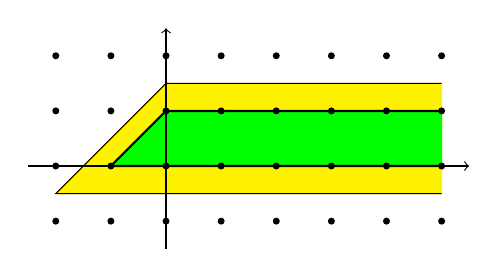
\begin{tikzpicture}[scale=0.7]
	
	\filldraw[yellow] (5,-0.5) -- (-2,-0.5) -- (0,1.5) -- (5,1.5) -- cycle;
	\filldraw[green] (5,0) -- (-1,-0) -- (0,1) -- (5,1) -- cycle;
	
	\foreach \x in {-2,...,5}
	\foreach \y in {-1,...,2}
	{
		\filldraw[fill=black] (\x,\y)  circle (1.5pt);
	}
	\draw[->] (-2.5,0) -- (5.5,0);
	\draw[->] (0,-1.5) -- (0,2.5);
	\draw (5,-0.5) -- (-2,-0.5) -- (0,1.5) -- (5,1.5); 
	\draw[thick] (5,0) -- (-1,-0) -- (0,1) -- (5,1);
	\end{tikzpicture}
\end{center}

The input is \verb|InhomIneqIH.in| ( \verb|InhomIneq.in| augmented by \verb|IntegerHull|). The data of the integer hull are found in \verb|InhomIneqIH.IntHull.out|:
\begin{Verbatim}
...
2 vertices of polyhedron:
-1 0 1
0 1 1

1 extreme rays of recession cone:
1 0 0

3 support hyperplanes of polyhedron (homogenized):
0 -1 1
0  1 0
1 -1 1
\end{Verbatim}

\subsection{Inhomogeneous congruences}\label{ChinRem}

We want to compute the nonnegative solutions of the simultaneous inhomogeneous congruences
\begin{align*}
	x_1 + 2x_2 &\equiv 3\pod 7,\\
	2x_1 + 2x_2 &\equiv 4\pod{13}
\end{align*}
in two variables. The input file \verb|InhomCong.in| is
\begin{Verbatim}
amb_space 2
constraints 2 symbolic
x[1] + 2x[2] ~ 3 (7);
2x[1] +  2x[2] ~ 4 (13);
\end{Verbatim}
This is an example of input of symbolic constraints. We use \verb|~| as the best ASCII character for representing the congruence sign $\equiv$.	

Alternatively one can use a matrix in the input As for which we must move the right hand side over to the left.
\begin{Verbatim}
amb_space 2
inhom_congruences 2
1 2 -3 7
2 2 -4 13
\end{Verbatim}
It is certainly harder to read.

The first vector list in the output:

\begin{Verbatim}
3 module generators:
0 54 1
1  1 1
80  0 1
\end{Verbatim}
Easy to check: if $(1,1)$ is a solution, then it must generate the module of solutions together with the generators of the intersections with the coordinate axes. Perhaps more difficult to find: 
\begin{Verbatim}
6 Hilbert basis elements of recession monoid:
0 91 0
1 38 0
3 23 0                                       1 vertices of polyhedron:
5  8 0                                       0 0 91
12  1 0
91  0 0
\end{Verbatim}
Strange, why is $(0,0,1)$, representing the origin in $\RR^2$, not listed as a vertex as well?
Well the vertex shown represents an extreme ray in the lattice $\EE$, and $(0,0,1)$ does not belong to $\EE$.

\begin{Verbatim}
2 extreme rays of recession cone:
0 91 0
91  0 0

3 support hyperplanes of polyhedron (homogenized)
0 0 1
0 1 0
1 0 0

1 congruences:
58 32 1 91
\end{Verbatim}
Normaliz has simplified the system of congruences to a single one.
\begin{Verbatim}
3 basis elements of generated lattice:
 1 0  33
 0 1 -32
 0 0  91
\end{Verbatim}
Again, don't forget that Normaliz prints a basis of the efficient lattice $\EE$.

\subsubsection{Lattice and offset}\label{offset_ex}

The set of solutions to the inhomogeneous system is an affine lattice in $\RR^2$. The lattice basis of $\EE$ above does not immediately let us write down the set of solutions in the form $w+L_0$ with a subgroup $L_0$, but we can easily transform the basis of $\EE$: $(1,1,1)$ is in $\EE$ and we use it to reduce the third column of the other two basis elements to $0$. Try the file \verb|InhomCongLat.in|:

\begin{Verbatim}
amb_space 2
offset
1 1
lattice 2
5 8
-12 -1
\end{Verbatim}


\subsubsection{Variation of the signs}\label{sign_ex}

Suppose we want to solve the system of congruences under the condition that both variables are negative (\verb|InhomCongSigns.in|): 

\begin{Verbatim}
amb_space 2
inhom_congruences 2
1 2 -3 7
2 2 -4 13
signs
-1 -1
\end{Verbatim}
The two entries of the sign vector impose the sign conditions $x_1\le 0$ and $x_2\le 0$.

From the output we see that the module generators are more complicated now:
\begin{Verbatim}
4 module generators:
-11   0 1
-4  -7 1
-2 -22 1
0 -37 1
\end{Verbatim}
The Hilbert basis of the recession monoid is simply that of the nonnegative case multiplied by $-1$.

\subsection{Integral closure and Rees algebra of a monomial ideal}\label{Rees}

Next, let us discuss the example \ttt{MonIdeal.in} (typeset in two columns):

\begin{Verbatim}
amb_space 5
rees_algebra 9
1 2 1 2                 1 0 3 4
3 1 1 3                 5 1 0 1
2 5 1 0                 2 4 1 5
0 2 4 3                 2 2 2 4
0 2 3 4
\end{Verbatim}
The input vectors are the exponent vectors of a monomial ideal $I$  in the ring $K[X_1,X_2,X_3,X_4]$. We want to compute the normalization of the Rees algebra of the ideal. In particular we can extract from it the integral closure of the ideal. Since we must introduce an extra variable $T$, we have \verb|amb_space 5|.  

In the Hilbert basis we see the exponent vectors of the $X_i$, namely the unit vectors with last component $0$. The vectors with last component $1$ represent the integral closure $\overline I$  of the ideal. There is a  vector with last component $2$, showing that the integral closure of $I^2$ is larger than~$\overline I^2$.
\begin{Verbatim}
16 Hilbert basis elements:
0 0 0 1 0
...
5 1 0 1 1
6 5 2 2 2

11 generators of integral closure of the ideal:
0 2 3 4
...
5 1 0 1
\end{Verbatim}
The output of the generators of $\overline I$ is the only place where we suppress the homogenizing variable for ``historic'' reasons. If we extract the vectors with last component $1$ from the extreme rays, then we obtain the smallest monomial ideal that has the same integral closure as $I$.
\begin{Verbatim}
10 extreme rays:
0 0 0 1 0
...
5 1 0 1 1
\end{Verbatim}
The support hyperplanes which are not just sign conditions describe primary decompositions of all the ideals $\overline{I^k}$ by valuation ideals. It is not hard to see that none of them can be omitted for large $k$ (for example, see: W. Bruns and G. Restuccia,  Canonical modules of Rees algebras. J. Pure Appl. Algebra 201, 189--203 (2005)).
\begin{Verbatim}
23 support hyperplanes:
0 0 0  0   1
0 ...
6 0 1  3 -13
\end{Verbatim}

\subsubsection{Only the integral closure of the ideal}

If only the integral closure of the ideal is to be computed, one can choose the input as follows (\verb|IntClMonId.in|):
\begin{Verbatim}
amb_space 4
vertices 9
1 2 1 2 1
...
2 2 2 4 1
cone 4
1 0 0 0
0 1 0 0
0 0 1 0
0 0 0 1
\end{Verbatim}

The generators of the integral closure appear as module generators in the output and the generators of the smallest monomial ideal with this integral closure are the vertices of the polyhedron.

\subsection{Starting from a binomial ideal}\label{binom_ex}

As an example, we consider the binomial ideal generated by
$$
X_1^2X_2-X_4X_5X_6,\ \ X_1X_4^2-X_3X_5X_6,\ \ X_1X_2X_3-X_5^2X_6.
$$
We want to find an embedding of the toric ring it defines and
the normalization of the toric ring. The input vectors are obtained as the differences of the two exponent vectors in the binomials. So the input ideal \verb+lattice_ideal.in+ is
\begin{Verbatim}
amb_space 6
lattice_ideal 3
2 1  0 -1 -1  -1
1 0 -1  2 -1  -1
1 1  1  0 -2  -1
\end{Verbatim}
In order to avoid special input rules for this case in which our object is not defined as a subset of an ambient space, but as a quotient of type \emph{generators/relations}, we abuse the name \verb|amb_space|: it determines the space in which the input vectors live.

We get the output
\begin{Verbatim}
6 original generators of the toric ring
\end{Verbatim}
namely the residue classes of the indeterminates.
\begin{Verbatim}
9 Hilbert basis elements
9 lattice points in polytope (Hilbert basis elements of degree 1)
\end{Verbatim}
So the toric ring defined by the binomials is not normal. Normaliz found the standard grading on the toric ring. The normalization is generated in degree $1$, too (in this case). 
\begin{Verbatim}
5 extreme rays
5 support hyperplanes

embedding dimension = 3
rank = 3 (maximal)
external index = 1
internal index = 1
original monoid is not integrally closed
\end{Verbatim}
We saw that already.
\begin{Verbatim}
size of triangulation   = 5
resulting sum of |det|s = 10

grading:
-2 1 1
\end{Verbatim}
This is the grading on the ambient space (or polynomial ring) defining the standard grading on our subalgebra. The enumerative data that follow are those of the normalization! 
\begin{Verbatim}
degrees of extreme rays:
1: 5  

Hilbert basis elements are of degree 1

multiplicity = 10

Hilbert series:
1 6 3 
denominator with 3 factors:
1: 3  

degree of Hilbert Series as rational function = -1

Hilbert polynomial:
1 3 5 
with common denominator = 1

rank of class group = 2
class group is free

***********************************************************************

6 original generators:
1 0 0
2 3 5
0 0 1
1 1 2
0 1 3
3 1 0
\end{Verbatim}
This is an embedding of the toric ring defined by the binomials. There are many choices, and Normaliz has taken one of them. You should check that the generators in this order satisfy the binomial equations. Turning to the ring theoretic interpretation, we can say that the toric ring defined by the binomial equations can be embedded into $K[Y_1,Y_2,Y_3]$ as a monomial subalgebra that is generated by $Y_1^0Y_2^0Y_3^1$,\dots,$Y_1^1Y_2^0Y_3^3$.

Now the generators of the normalization:
\begin{Verbatim}
9 lattice points in polytope (Hilbert basis elements of degree 1):    
                                          5 extreme rays:
0 0 1                                     0 0 1
0 1 3                                     0 1 3
1 0 0                                     1 0 0
1 1 2                                     2 3 5
1 2 4                                     3 1 0
2 1 1
2 2 3                                    5 support hyperplanes:
2 3 5                                    0   0 15
3 1 0                                    0   1 0
                                         1   0 0
                                         2  -3 1
                                         5 -15 7

0 further Hilbert basis elements of higher degree:	  
\end{Verbatim}


%%%%%%%%%%%%%%%%%%%%%%%%%%%%%  INPUT  %%%%%%%%%%%%%%%%%%%%%%%%%%%%%
\section{The input file}\label{input}

The input file \ttt{<project>.in} consists of one or
several items. There are several types of items:

\begin{arab}
	\item definition of the ambient space,
	\item matrices with integer or rational entries (depending on the type),
	\item vectors with integer entries,
	\item constraints in tabular or symbolic format,
	\item a polynomial,
	\item computation goals and algorithmic variants,
	\item numerical parameters,
	\item number field definitions,
	\item comments.
\end{arab}

An item cannot include another item. In particular, comments can only be included between other items, but not within another item. Matrices and vectors can have two different formats, plain and formatted.

Matrices and vectors are classified by the following attributes:
\begin{arab}
	\item generators, constraints, accessory,
	\item cone/polyhedron, (affine) lattice,
	\item homogeneous, inhomogeneous.
\end{arab} 
In this classification, equations are considered as constraints on the lattice because Normaliz treats them as such -- for good reason: it is very easy to intersect a lattice with a hyperplane.

The line structure is irrelevant for the interpretation of the input, but it is advisable to use it for the readability of the input file.

The input syntax of Normaliz 2 can still be used. It is explained in Appendix \ref{OldSyntax}.

\subsection{Input items}

\subsubsection{The ambient space and lattice}

The ambient space is specified as follows:
\begin{Verbatim}
amb_space <d>
\end{Verbatim}
where \ttt{<d>} stands for the dimension $d$ of the ambient vector space $\RR^d$ in which the geometric objects live.  The \emph{ambient lattice} $\AA$ is set to $\ZZ^d$.

Alternatively one can define the ambient space implicitly by
\begin{Verbatim}
amb_space auto
\end{Verbatim}
In this case the dimension of the ambient space is determined by Normaliz from the first formatted vector or matrix in the input file. It is clear that any input item that requites the knowledge of the dimension can only follow the first formatted vector or matrix.

\emph{In the following the letter $d$ will always denote the dimension set with} \verb|amb_space|.


An example:
\begin{Verbatim}
amb_space 5
\end{Verbatim}
indicates that polyhedra and lattices are subobjects of $\RR^5$. The ambient lattice is $\ZZ^5$. 

\emph{The first non-comment input item must specify the ambient space.}

\subsubsection{Plain vectors}

A plain vector is built as follows:
\begin{Verbatim}
<T>
<x>
\end{Verbatim}
Again \ttt{<T>} denotes the type and \ttt{<x>} is the vector itself. The number of components is determined by the type of the vector and the dimension of the ambient space. At present, all vectors have length $d$.

Example:
\begin{Verbatim}
grading
1 0 0
\end{Verbatim}

Normaliz allows also the input of sparse vectors. Sparse input is signalized by the key word \verb|sparse| as the first entry. It is followed by entries of type \verb|<col>:<val>| where \verb|<col>| denotes the column and \verb|<val>| the value in that column. (The unspecified columns have entry $0$.) A sparse vector is terminated by the character \verb|;| . 

Example:
\begin{Verbatim}
grading
sparse 1:1;
\end{Verbatim}


For certain vectors there also exist shortcuts. Examples:
\begin{Verbatim}
total_degree
unit_vector 25
\end{Verbatim}


\subsubsection{Formatted vectors}

A formatted vector is built as follows:
\begin{Verbatim}
<T>
[ <x> ]
\end{Verbatim}
where \ttt{<T>} denotes the type and \ttt{<x>} is the vector itself. The components can be separated by white space, commas or semicolons. An example showing all possibilities (not recommended):
\begin{Verbatim}
grading
[1,0; 0 5]
\end{Verbatim}

\subsubsection{Plain matrices}

A plain matrix is built as follows:
\begin{Verbatim}
<T> <m>
<x_1>
...
<x_m>
\end{Verbatim}
Here \ttt{<T>} denotes the type of the matrix, \ttt{<m>} the number of rows, and \ttt{<x\_1>},...,\ttt{<x\_m>} are the rows. Some types allow rational and floating point matrix entries, others are restricted to integers; see Sections \ref{rational_input} and \ref{decimal_input}.

The number of columns is implicitly defined by the dimension of the ambient space and the type of the matrix. Example (with \verb|amb_space 3|):
\begin{Verbatim}
cone 3
1/3 2 3
4 5 6
11 12/7 13/21
\end{Verbatim}

Normaliz allows the input of matrices in transposed form:
\begin{Verbatim}
<T> transpose <n>
<x_1>
...
<x_m>
\end{Verbatim}
Note that \verb|<n>| is now the number of \emph{columns} of the matrix that follows it (assumed to be the number of input vectors). The number of rows is determined by the dimension of the ambient space and the type of the matrix.  Example:
\begin{Verbatim}
cone transpose 3
1  0   3/2
0 1/9   4
\end{Verbatim}
is equivalent to
\begin{Verbatim}
cone 3
 1  0
 0 1/9
3/2 4
\end{Verbatim}

Like vectors, matrices have a sparse input variant, again signalized by the key word \verb|sparse|. The rows are sparse vectors with entries \verb|<col>:<val>|, and each row is concluded by the character \verb|;|.

Example:
\begin{Verbatim}
inequalities 3 sparse
1:1;
2:1;
3:1;
\end{Verbatim}
chooses the $3\times 3$ unit matrix as a matrix of type \verb|inequalities|. Note that also in case of transposed matrices, sparse entry is row by row.

\emph{Matrices may have zero rows.} Such empty matrices like
\begin{Verbatim}
inhom_inequalities 0
\end{Verbatim}

can be used to make the input inhomogeneous (Section \ref{inhom_inp}) or to avoid the automatic choice of the positive orthant in certain cases (Section \ref{default}). (The empty \verb|inhom_inequalities| have both effects simultaneously.) Apart from these effects, empty matrices have no influence on the computation.

\subsubsection{Formatted matrices}

A formatted matrix is built as follows:
\begin{Verbatim}
<T>
[ [<x_1>]
...
[<x_m>]  ]
\end{Verbatim}
Here \ttt{<T>} denotes the type of the matrix and \verb|<x_1>|,\dots,\verb|<x_m>| are vectors. Legal separators are white space, commas and semicolons. An example showing all possibilities (not really recommended):
\begin{Verbatim}
cone [
[ 2 1][3/7 4];
[0 1],
[9 10] [11 12/13]
]
\end{Verbatim} 
Similarly as plain matrices, formatted matrices can be given in transposed form, and they can be empty.

\subsubsection{Constraints in tabular format}\label{const_syntax}

This input type is somewhat closer to standard notation than the encoding of constraints in matrices. The general type of equations and inequalities is
\begin{Verbatim}
<x> <rel> <rhs>;
\end{Verbatim}
where \verb|<x>| denotes a vector of length $d$, \verb|<rel>| is one of the relations \verb|=, <=, >=, <, >| and \verb|<rhs>| is a number.

Congruences have the form
\begin{Verbatim}
<x> ~ <int> (<mod>);
\end{Verbatim}
where \verb|<mod>| is a nonzero integer.

Examples:
\begin{Verbatim}
1/2 -2 >= 0.5
1 -1/7 = 0
-1 1 ~ 7 (9)
\end{Verbatim}

Note: all numbers and relation signs must be separated by white space.

\subsubsection{Constraints in symbolic format}\label{symb_syntax}

This input type is even closer to standard notation than the encoding of constraints in matrices or in tabular format. It is especially useful if the constraints are sparse. Instead of assigning a value to a coordinate via its position in a vector, it uses coordinates named \verb|x[<n>]| where \verb|<n>| is the index of the coordinate. The index is counted from $1$. 

 The general type of equations and inequalities is
\begin{Verbatim}
<lhs> <rel> <rhs>;
\end{Verbatim}
where \verb|<lhs>| and \verb|<rhs>| denote affine linear function of the \verb|x<n>| with rational coefficients. 
As above, \verb|<rel>| is one of the relations \verb|=, <=, >=, <, >|. (Both \verb|<lhs>| and \verb|<rhs>| must be nonempty.) Note the terminating semicolon.

Congruences have the form
\begin{Verbatim}
<lhs> ~ <rhs> (<mod>);
\end{Verbatim}
where \verb|<mod>| is a nonzero integer and \verb|<lhs>| and \verb|<rhs>| are affine linear functions with integer coefficients.

Examples:
\begin{Verbatim}
1/3x[1] >= 2x[2] + 5;
x[1]+1=1/4x[2] ;
-x[1] + x[2] ~ 7 (9);
\end{Verbatim}

There is no need to insert white space for separation, but it may be inserted anywhere where it does not disrupt numbers or relation signs.

\subsubsection{Polynomials}\label{poly_input}

For the computation of weighted Ehrhart series and integrals Normaliz needs the input of a polynomial with rational coefficients. The polynomial is first read as a string. For the computation the string is converted by the input function of CoCoALib \cite{CoCoA}. Therefore any string representing a valid CoCoA expression is allowed. However the names of the indeterminates are fixed: \verb|x[1]|,\dots,\verb|x[<N>| where \verb|<N>]| is the value of \verb|amb_space|. The polynomial must be concluded by a semicolon.

Example:
\begin{Verbatim}
(x[1]+1)*(x[1]+2)*(x[1]+3)*(x[1]+4)*(x[1]+5)*
(x[2]+1)*(x[3]+1)*(x[4]+1)*(x[5]+1)*(x[6]+1)*(x[7]+1)*
(x[8]+1)*(x[8]+2)*(x[8]+3)*(x[8]+4)*(x[8]+5)*1/14400;

(x[1]*x[2]*x[3]*x[4])^2*(x[1]-x[2])^2*(x[1]-x[3])^2*
(x[1]-x[4])^2*(x[2]-x[3])^2*(x[2]-x[4])^2*(x[3]-x[4])^2;
\end{Verbatim}

\subsubsection{Rational numbers}\label{rational_input}

Rational numbers are allowed in input matrices, but not in all. They are \emph{not} allowed in vectors and in matrices containing lattice generators and in congruences, namely in
\begin{Verbatim}
lattice     cone_and_lattice   offset         open_facets
congruences inhom_congruences  rees_algebra   lattice_ideal
grading     dehomogenization   signs          strict_signs
\end{Verbatim}
They are allowed in \verb|saturation| since it defines the intersection of the vector space generated by the rows of the matrix with the integral lattice.

Aavoid negative numbers as denominators.

Normaliz first reduces the input numbers to lowest terms. Then each row of a matrix is multiplied by the least common multiple of the denominators of its entries. In all applications in which the original monoid generators play a role, one should use only integers in input matrices to avoid any ambiguity.

\subsubsection{Decimal fractions and floating point numbers}\label{decimal_input}

Normaliz accepts decimal fractions and floating point numbers in its input files. These are precisely converted to ordinary fractions (or integers). Examples:
\begin{Verbatim}
1.1 --> 11/10    0.5 --> 1/2    -.1e1 --> -1
\end{Verbatim}
It is not allowed to combine an ordinary fraction and a decimal fraction in the same number. In other words, expressions like \verb|1.0/2| are not allowed.

\subsubsection{Numbers in algebraic extensions of $\QQ$}\label{numberfield_input}

Their format is explained in Section \ref{alg_ex} together with the definition of number fields.

\subsubsection{Computation goals and algorithmic variants}\label{subsecGoals}

These are single or compound words, such as
\begin{Verbatim}
HilbertBasis
Multiplicity
\end{Verbatim}
The file can contain several computation goals, as in this example.

\subsubsection{Comments}

A comment has the form
\begin{Verbatim}
/* <text> */
\end{Verbatim}
where \ttt{<text>} stands for the text of the comment. It can have arbitrary length and stretch over several lines. Example:
\begin{Verbatim}
/* This is a comment
*/
\end{Verbatim}
Comments are only allowed at places where also a new keyword would be allowed, especially not between the entries of a matrix or a vector. Comments can not be nested.

\subsubsection{Restrictions}

Input items can almost freely be combined, but there are some restrictions:

\begin{arab}
	\item The types
	\begin{center}
		\ttt {cone, cone\_and\_lattice, polytope, rees\_algebra}	
	\end{center}
	exclude each other mutually.
	\item The input type \verb|subspace| excludes \verb|polytope| and \verb|rees_algebra|.
	\item The types
	\begin{center}
		\ttt {lattice}, \ttt{saturation}, \ttt{cone\_and\_lattice}	
	\end{center}
	exclude each other mutually.
	\item \verb|polytope| can not be combined with \verb|grading|.
	\item The only type that can be combined with \ttt{lattice\_ideal} is \ttt{grading}.
	\item The following types cannot be combined with inhomogeneous types or \verb|dehomogenization|:
	\begin{center}
		\ttt{polytope, rees\_algebra, excluded\_faces}
	\end{center}
	
	\item The following types cannot be combined with inhomogeneous types:
	\begin{center}
		\ttt{dehomogenization, support\_hyperplanes, extreme\_rays.}
	\end{center}
	
	\item Special restrictions apply for the input types \verb|lattice_odeal| and \verb|open_facets|; see Sections \ref{relations} and \ref{open_facets}.
	
	\item For restrictions that apply to algebraic polyhedra see Section \ref{Algebraic}.
\end{arab}

A non-restriction: the same type can appear several times. This is useful if one wants to combine different formats, for example
\begin{Verbatim}
inequalities 2 sparse
1:1;
1:1 3:-1;
inequalities 2
1 1 0 1
1 -1 -1 0
\end{Verbatim}

\subsubsection{Homogeneous and inhomogeneous input}\label{inhom_inp}

Apart from the restrictions listed in the previous section, homogeneous and inhomogeneous types can be combined as well as generators and constraints. A single inhomogeneous type or \verb|dehomogenization| in the input triggers an inhomogeneous computation. The input item of inhomogeneous type may be an empty matrix.

\subsubsection{Default values}\label{default}

If there is no lattice defining item, Normaliz (virtually) inserts the the unit matrix as an input item of type \ttt{lattice}. If there is no cone defining item, the unit matrix is (additionally) inserted as an input item of type \ttt{cone}.

If the input is inhomogeneous, then Normaliz provides default values for vertices and the offset as follows:
\begin{arab}
	\item If there is an input matrix type \verb|lattice|, but no \ttt{offset}, then the offset $0$ is inserted.
	\item If there is an input matrix of type cone, but no \ttt{vertices}, then the vertex $0$ is inserted. 
\end{arab}

\textbf{An important point.}\enspace If the input does not contain any cone generators or inequalities, Normaliz automatically assumes that you want to compute in the positive orthant. In order to avoid this choice you can add an empty matrix of inequalities. This will not affect the results, but avoid the sign restriction.



\subsubsection{Normaliz takes intersections (almost always)}

The input may contain several cone defining items and several lattice defining items.

The sublattice $L$  defined by the lattice input items is the \emph{intersection} of the sublattices defined by the single items. The polyhedron $P$ is defined as the intersection of all polyhedra defined by the single  polyhedron defining items. The object then computed by Normaliz is
$$
P\cap L.
$$

There are three notable exceptions to the rule that Normaliz takes intersections:
\begin{arab}
	\item \verb|vertices| and \verb|cone| form a unit. Together they define a polyhedron.
	\item The same applies to \verb|offset| and \verb|lattice| that together define an affine lattice.
	\item The \verb|subspace| is added to \verb|cone| or \verb|cone_and_lattice|.
\end{arab}

\subsection{Homogeneous generators}

\subsubsection{Cones}\label{cone_synt}

The main type is \verb|cone|. The other two types are added for special computations.

\begin{itemize}
	\itemtt[cone] is a matrix with $d$ columns. Every row represents a vector, and they define the cone generated by them. Section \ref{cone_ex}, \verb|2cone.in|

	\itemtt[subspace] is a matrix with $d$ columns. The linear subspace generated by the rows is added to the cone. Section \ref{subspace}.
	
	\itemtt[polytope] is a matrix with $d-1$ columns. It is internally converted to \verb|cone| extending each row by an entry $1$.  Section \ref{polytope_ex}, \verb|polytope.in|. This input type automatically sets \verb|NoGradingDenom| and defines the grading $(0,\dots,0,1)$. Not allowed in combination with inhomogeneous types.
	
	\itemtt[rees\_algebra] is a matrix with $d-1$ columns. It is internally converted to type \verb|cone| in two steps: (i) each row is extended by an entry $1$ to length $d$. (ii) The first $d-1$ unit vectors of length $d$ are appended. Section \ref{Rees}, \verb|MonIdeal.in|. Not allowed in combination with inhomogeneous types.
	
	\itemtt[extreme\_rays] is a matrix with $d$ columns. It requires homogeneous input. It is the input type for precomputed extreme rays. Normaliz takes their correctness for granted, but they do not define the cone. Section \ref{extrays_ex}, \verb|2cone_extt.in|.
\end{itemize}

Moreover, it is possible to define a cone and a lattice by the same matrix:

\begin{itemize}
	\itemtt[cone\_and\_lattice] The vectors of the matrix with $d$ columns define both a cone and a lattice. Section \ref{normalization_ex}, \verb|A443.in|.
	
	If \verb|subspace| is used in combination with \verb|cone_and_lattice|, then the sublattice generated by its rows is added to the lattice generated by \verb|cone_and_lattice|.
\end{itemize}


The Normaliz 2 types \verb|integral_closure| and \verb|normalization| can still be used. They are synonyms for \verb|cone| and \verb|cone_and_lattice|, respectively.

\subsubsection{Lattices}

There are $3$ types:

\begin{itemize}
	\itemtt[lattice] is a matrix with $d$ columns. Every row represents a vector, and they define the lattice generated by them. Section \ref{latt_ex}, \verb|3x3magiceven_lat.in|
	
	\itemtt[saturation] is a matrix with $d$ columns. Every row represents a vector, and they define the  lattice $U\cap \ZZ^d$ where $U$ is the subspace generated by them. Section \ref{latt_ex}, \verb|3x3magic_sat.in|. (If the vectors are integral, then $U\cap \ZZ^d$ is the saturation of the ?attice generated by them.)
	
	\itemtt[cone\_and\_lattice] See Section \ref{cone_synt}.
\end{itemize}


\subsection{Homogeneous Constraints}

The coefficients $\xi_i$ of the constraints are rational numbers unless indicated otherwise.

\subsubsection{Cones} \label{HomConstrCone}

\begin{itemize}
	\itemtt[inequalities] is a matrix with $d$ columns. Every row $(\xi_1,\dots,\xi_d)$ represents a homogeneous inequality
	$$
	\xi_1x_1+\dots+\xi_dx_d\ge 0
	$$
	for the vectors $(x_1,\dots,x_d)\in\RR^d$. Sections \ref{ineq_ex}, \ref{rat_ineq} , \verb|2cone_ineq.in|, \verb|poly_ineq.in|
	
	\itemtt[signs] is a vector with $d$ entries in $\{-1,0,1\}$.
	It stands for a matrix of type \verb|inequalities| composed of the sign inequalities $x_i\ge 0$ for the entry $1$ at the $i$-th component and the inequality $x_i\le 0$ for the entry $-1$. The entry $0$ does not impose an inequality. See \ref{sign_ex}, \verb|InhomCongSigns.in|.
	
	\itemtt[nonnegative] It stands for a vector of type \verb|sign| with all entries equal to $1$. See Section \ref{Condorcet}, \verb|Condorcet.in|.
	
	\itemtt[excluded\_faces]  is a matrix with $d$ columns. Every row $(\xi_1,\dots,\xi_d)$ represents an inequality
	$$
	\xi_1x_1+\dots+\xi_dx_d> 0
	$$
	for the vectors $(x_1,\dots,x_d)\in\RR^d$. It is considered as a homogeneous input type though it defines inhomogeneous inequalities. The faces of the cone excluded by the inequalities are excluded from the Hilbert series computation, but \verb|excluded_faces| behaves like \verb|inequalities| in every other respect . 
	Section \ref{excluded_ex}, \verb|CondorcetSemi.in|.
	
	\itemtt[support\_hyperplanes] is a matrix with $d$ columns. It requires homogeneous input. It is the input type for precomputed support hyperplanes. Note that it overrides all other inequalities in the input, but \verb|excluded_faces| still exclude the faces defined by them. Section \ref{supphyp_ex}, \verb|2cone_supp.in|.
\end{itemize}

\subsubsection{Lattices}

\begin{itemize}
	\itemtt[equations] is a matrix with $d$ columns. Every row $(\xi_1,\dots,\xi_d)$ represents an equation
	$$
	\xi_1x_1+\dots+\xi_dx_d= 0
	$$
	for the vectors $(x_1,\dots,x_d)\in\RR^d$. Section \ref{eq_ex}, \verb|3x3magic.in|
	
	\itemtt[congruences] is a matrix with $d+1$ columns. Each row $(\xi_1,\dots,\xi_d,c)$ represents a congruence
	$$
	\xi_1z_1+\dots+\xi_dz_d\equiv 0 \mod c, \qquad \xi_i,c\in\ZZ,
	$$
	for the elements $(z_1,\dots,z_d)\in\ZZ^d$. Section \ref{cong_ex}, \verb|3x3magiceven.in|.
\end{itemize}

\subsection{Inhomogeneous generators}

\subsubsection{Polyhedra}

\begin{itemize}
	\itemtt[vertices] is a matrix with $d+1$ columns. Each row $(p_1,\dots,p_d,q)$, $q>0$, specifies a generator of a polyhedron (not necessarily a vertex), namely
	$$
	v_i=\biggl(\frac{p_{1}}{q},\dots,\frac{p_{n}}{q}\biggr), \qquad p_i\in\QQ,q\in\QQ_{>0},
	$$
	Section \ref{polyh_ex}, \verb|InhomIneq_gen.in|
	
	\textbf{Note:}\enspace \verb|vertices| and \verb|cone| together define a polyhedron. If \verb|vertices| is present in the input, then the default choice for \verb|cone| is the empty matrix.
\end{itemize}

The format of \verb|vertices| was introduced when Normaliz only accepted integer numbers in its input. There is no need for an extra denominator anymore, but for backwared compatibility the format has not been changed.

The Normaliz 2 input type \verb|polyhedron| can still be used.

\subsubsection{Affine lattices}

\begin{itemize}
	\itemtt[offset] is a vector with $d$ integer entries. It defines the origin of the affine lattice.
	Section \ref{offset_ex}, \verb|InhomCongLat.in|.
\end{itemize}

\textbf{Note:}\enspace \verb|offset| and \verb|lattice| (or \verb|saturation|) together define an affine lattice. If \verb|offset| is present in the input, then the default choice for \verb|lattice| is the empty matrix.

\subsection{Inhomogeneous constraints}

\subsubsection{Polyhedra}

\begin{itemize}
	\itemtt[inhom\_inequalities] is a matrix with $d+1$ columns. We consider inequalities
	$$
	\xi_1x_1+\dots+\xi_dx_d\ge \eta,
	$$
	rewritten as
	$$
	\xi_1x_1+\dots+\xi_dx_d+(-\eta) \ge 0
	$$
	and then represented by the input vectors
	$$
	(\xi_1,\dots,\xi_d,-\eta).
	$$
	Section \ref{inhom_ineq_ex}, \verb|InhomIneq.in|.
	
	\itemtt[strict\_inequalities] is a matrix with $d$ columns. We consider inequalities
	$$
	\xi_1x_1+\dots+\xi_dx_d\ge 1,
	$$
	represented by the input vectors
	$$
	(\xi_1,\dots,\xi_d).
	$$
	Section \ref{strict_ex}, \verb|2cone_int.in|.
	
	\itemtt[strict\_signs] is a vector with $d$ components in $\{-1,0,1\}$. It is the ''strict'' counterpart to \verb|signs|. An entry $1$ in component $i$ represents the inequality $x_i>0$, an entry $-1$ the opposite inequality, whereas $0$ imposes no condition on $x_i$. \ref{strict_signs_ex}, \verb|Condorcet_one.in|
\end{itemize}

\subsubsection{Affine lattices}

\begin{itemize}
	\itemtt[inhom\_equations] is a matrix with $d+1$ columns. We consider equations
	$$
	\xi_1x_1+\dots+\xi_dx_d= \eta, 
	$$
	rewritten as
	$$
	\xi_1x_1+\dots+\xi_dx_d+(-\eta) = 0
	$$
	and then represented by the input vectors
	$$
	(\xi_1,\dots,\xi_d,-\eta).
	$$
	See \ref{inhom_eq_ex}\verb|NumSemi.in|.
	
	\itemtt[inhom\_congruences] We consider a matrix with $d+2$ columns. Each  the row $(\xi_1,\dots,\xi_d,-\eta,c)$ represents a congruence
	$$
	\xi_1z_1+\dots+\xi_dz_d\equiv \eta \mod c, \qquad \xi_i,\eta,c\in\ZZ,
	$$
	for the elements $(z_1,\dots,z_d)\in\ZZ^d$. Section \ref{ChinRem}, \verb|InhomCongSigns.in|.
\end{itemize}

\subsection{Tabular constraints}

\begin{itemize}
	\itemtt[constraints] allows the input of equations, inequalities and congruences in a format that is close to standard notation. As for matrix types the keyword \verb|constraints| is followed by the number of constraints. The syntax of tabular constraints has been described in Section \ref{cone_synt}. If $(\xi_1,\dots,\xi_d)$ is the vector on the left hand side and $\eta$ the number on the right hand side, then the constraint defines the set of vectors $(x_1,\dots,x_d)$ such that the relation
	$$
		\xi_1x_1+\dots +\xi_dx_d \texttt{ rel } \eta
	$$
	is satisfied, where \verb|rel| can take the values $=,\leq,\geq,<,>$ with the represented by input strings \verb|=,<=,>=,<,>|, respectively.
	
	Constraints with the  relations $>$ and $<$ are converted to \verb|strict_inequalities|.
	
	The input string \verb|~| represents a congruence $\equiv$ and requires the additional input of a modulus. It represents the congruence
	$$
	\xi_1x_1+\dots \xi_dx_d \equiv \eta \pmod c. 
	$$
	Sections \ref{strict_ex}, \verb|2cone_int.in|,  \ref{cong_ex}, \ttt{3x3magiceven.in}, \ref{inhom_ineq_ex}, \verb|InhomIneq.in|.
\end{itemize}

A right hand side $\neq 0$ makes the input inhomogeneous, as well as the relations $<$ and $>$. Strict inequalities are always understood as conditions for integers. So
$$
\xi_1x_1+\dots +\xi_dx_d < \eta
$$
is interpreted as
$$
\xi_1x_1+\dots \xi_dx_d \le \eta-1,
$$


\subsubsection{Forced homogeneity}

It is often more natural to write constraints in inhomogeneous form, even when one wants the computation to be homogeneous. The type \verb|constraints| does not allow this. Therefore we have introduced
\begin{itemize}
	\itemtt[hom\_constraints] for the input of equations, non-strict inequalities and congruences in the same format as \verb|constraints|, except that these constraints are meant to be for a homogeneous computation. It is clear that the left hand side has only $d-1$ entries now. See Section \ref{rat_ineq}, \verb|poly_hom_const.in|.
\end{itemize}

\subsection{Symbolic constraints}

The input syntax is

\begin{itemize}
	\itemtt[constraints <n> symbolic] where \verb|<n>| is the number of constraints in symbolic form that follow.
\end{itemize}

The constraints have the form described in Section \ref{symb_syntax}. Note that every symbolic constraint (including the last) must be terminated by a semicolon.

See \ref{inhom_eq_ex}, \verb|NumSemi.in|, \ref{ChinRem}, \verb|InhomCong.in|.

The interpretation of homogeneity follows the same rules as for tabular constraints. The variant \verb|hom_constraints| is allowed and works as for tabular constraints.


\subsection{Relations}\label{relations}

Relations do not select a
sublattice of $\ZZ^d$ or a subcone of $\RR^d$, but define a
monoid as a quotient of $\ZZ_+^d$ modulo a system of
congruences (in the semigroup sense!).

The rows of the input matrix of this type are interpreted as
generators of a subgroup $U\subset\ZZ^d$, and Normaliz computes an affine monoid and its normalization  as explained in Section \ref{binomials}.

Set $G=\ZZ^d/U$ and $L=G/\textup{torsion}(G)$. Then the ambient lattice
is $\AA=\ZZ^r$, $r=\rank L$, and the efficient lattice is $L$, realized
as a sublattice of $\AA$. Normaliz computes the image of $\ZZ^d_+$ in $L$ and its normalization.

\begin{itemize}
	\itemtt[lattice\_ideal] is a matrix with $d$ columns containing the generators of the subgroup $U$. Section \ref{binom_ex}, \verb|lattice_ideal.in|.
\end{itemize}

The type \ttt{lattice\_ideal} cannot be combined with any other input type (except
\ttt{grading})---such a combination would not make sense. (See Section \ref{grad_lattid} for the use of a grading in this case.)

\subsection{Unit vectors}\label{unit_vectors}

A grading or a dehomogenization is often given by a unit vector:
\begin{itemize}
\itemtt[unit\_vector <n>]  represents the $n$th unit vector in $\RR^d$ where $n$ is the number given by \verb|<n>|.
\end{itemize}
This shortcut cannot be used as a row of a matrix. It can be used whenever a single vector is asked for, namely after \verb|grading|, \verb|dehomogenization|, \verb|signs| and \verb|strict_signs|. See Section \ref{rational}, \verb|rational.in|

\subsection{Grading}\label{grading}

This type is accessory. A $\ZZ$-valued grading can be specified in two ways:
\begin{arab}
	\item \emph{explicitly} by including a grading in the input, or
	\item \emph{implicitly}. In this case Normaliz checks whether
	the extreme integral generators of the monoid lie in an
	(affine) hyperplane $A$ given by an equation $\lambda(x)=1$ with a $\ZZ$-linear form $\lambda$. If so, then  $\lambda$ is used as the grading.\smallskip
	
	\emph{Implicit gradings are only possible for homogeneous computations.}\smallskip
	
	If the attempt to find an implicit grading causes an arithmetic overflow and \texttt{verbose} has been set (say, by the option\texttt{-c}), then Normaliz issues the warning
	\begin{Verbatim}
	Giving up the check for a grading
	\end{Verbatim}
	If you really need this check, rerun Normaliz with a bigger integer type.
\end{arab}

Explicit definition of a grading:
\begin{itemize}
	\itemtt[grading] is a vector of length $d$ representing the linear form that gives the grading. Section \ref{rational}, \verb|rational.in|.
	
	\itemtt[total\_degree] represents a vector of length $d$ with all entries equal to $1$. Section \ref{Condorcet}, \verb|Condorcet.in|.
\end{itemize}

Before Normaliz can apply the degree, it must be restricted
to the effective lattice $\EE$. Even if the entries of the
grading vector are coprime, it often happens that all degrees
of vectors in $\EE$ are divisible by a greatest common divisor
$ g>1$. Then $g$ is extracted from the degrees, and it will
appear as \ttt{denominator} in the output file.

Normaliz checks whether all generators of the (recession) monoid have
positive degree (after passage to the quotient modulo the unit group in the nonpointed case).
Vertices of polyhedra may have degrees $\le 0$.

\subsubsection{With \ttt{lattice\_ideal} input} \label{grad_lattid}

In this case the unit vectors correspond to generators of the
monoid. Therefore the degrees assigned to them must be
positive. Moreover, the vectors in the input represent binomial
relations, and these must be homogeneous. In other words, both
monomials in a binomial must have the same degree. This amounts
to the condition that the input vectors have degree $0$.
Normaliz checks this condition.

\subsection{Dehomogenization}

Like \verb|grading| this is an accessory type.

Inhomogeneous input for objects in $\RR^d$ is homogenized by an additional coordinate and then computed in $\RR^{d+1}$, but with the additional condition $x_{d+1}\ge 0$, and then dehomogenizing all results: the substitution $x_{d+1}=1$ acts as the \emph{dehomogenization}, and the inhomogeneous input types implicitly choose this dehomogenization.

Like the grading, one can define the dehomogenization explicitly:
\begin{itemize}
	\itemtt[dehomogenization] is a vector of length $d$ representing the linear form $\delta$.
\end{itemize}

The dehomogenization can be any linear form $\delta$  satisfying the condition $\delta(x)\ge 0$ on the cone that is truncated. (In combination with constraints, the condition $\delta(x)\ge 0$ is automatically satisfied since $\delta$ is added to the constraints.)

The input type \verb|dehomogenization| can only be combined with homogeneous input types, but makes the computation inhomogeneous, resulting in inhomogeneous output. The polyhedron computed is the intersection of the cone $\CC$ (and the lattice $\EE$) with the hyperplane given by $\delta(x)=1$, and the recession cone is $\CC\cap\{x:\delta(x)=0\}$.

A potential application is the adaptation of other input formats to Normaliz. The output must then be interpreted accordingly.

Section \ref{dehom_ex}, \verb|dehomogenization.in|.

\subsection{Open facets}\label{open_facets}

The input type \verb|open_facets| is similar to \verb|strict_inequalities|. However, it allows to apply strict inequalities that are not yet known. This makes only sense for simplicial polyhedra where a facet can be identified by the generator that does \emph{not} lie in it.

\verb|open_facets| is a vector with entries $\in \{0,1\}$.

The restrictions for the use of open facets are the following:
\begin{arab}
\item Only the input types \verb|cone,| \verb|vertices| and \verb|grading| can appear together with \verb|open_facets|.
\item The vectors in \verb|cone| are linearly independent.
\item There is at most one vertex.
\end{arab}
The number of vectors in \verb|cone| may be smaller than $d$, but \verb|open_facets| must have $d$ entries.


\verb|open_facets| make the computation inhomogeneous. They are interpreted as follows. Let $v$ be the vertex---if there are no \verb|vertices|, then $v$ is the origin. The shifted $C'=v+C$ is cut out by affine-linear inequalities $\lambda_i(x)\ge 0$ with coprime integer coefficients. We number these in such a way that $\lambda_i(v+c_i)\neq 0$ for the generators $c_i$ of $C$ (in the input order), $i=1,\dots,n$. Then all subsequent computations are applied to the shifted cone $C''=v'+C$ defined by the inequalities
$$
\lambda_i(x)\ge u_i
$$
where the vector $(u_1,\dots,u_d)$ is given by \verb|open_facets|. (If $\dim C<d$, then the entries $u_j$ with $j> \dim C$ are ignored.) 

That $1$ indicates `open'' is in accordance with its use for the disjoint decomposition; see Section \ref{Disjoint}. Section \ref{LattPointsFPE} discusses an example.

\subsection{Coordinates for projection}

The coordinates of a projection of the cone can be chosen by
\begin{itemize}
	\itemtt[projection\_coordinates]. It is a $0$-$1$ vector of length $d$.
\end{itemize}
The entries $1$ mark the coordinates of the image of the projection. The other coordinates give the kernel of the projection. See Section \ref{Proj_cone} for an exasmple.

\subsection{Numerical parameters}

Certain numerical parameters used by Normaliz can (only) be set in the input file. 

\subsubsection{Degree bound for series expansion}

It can be set by
\begin{Verbatim}
expansion_degree <n>
\end{Verbatim}
where \verb|<n>| is the number of coefficients to be computed and printed. See Section \ref{expansion}.

\subsubsection{Number of significant coefficients of the quasipolynomial}

It can be set by
\begin{Verbatim}
nr_coeff_quasipol <n>
\end{Verbatim}
where \verb|<n>| is the number of highest coefficients to be printed. See Section \ref{highest_coeff}.

\subsubsection{Codimension bound for the face lattice}

It can be set by
\begin{Verbatim}
face_codim_bound <n>
\end{Verbatim}
where \verb|<n>| is the bound for the codimension of the faces to be computed.


\subsection{Pointedness}

Since version 3.1 Normaliz can also compute nonpointed cones and polyhedra without vertices.

\subsection{The zero cone}\label{zero}

The zero cone with an empty Hilbert basis is a legitimate
object for Normaliz. Nevertheless a warning message is issued
if the zero cone is encountered.

\section{Computation goals and algorithmic variants}\label{Goals}

The library \verb|libnormaliz| contains a class \verb|ConeProperties| that collects computation goals, algorithmic variants and additional data that are used to control the work flow in \verb|libnormaliz| as well as the communication with other programs. The latter are not important for the Normaliz user, but are listed as a reference for \verb|libnormaliz|. See Appendix \ref{libnorm} for a description of \verb|libnormaliz|.

All computation goals and algorithmic variants can be communicated to Normaliz in two ways:
\begin{arab}
	\item in the input file, for example \verb|HilbertBasis|,
	\item via a verbatim command line option, for example \verb|--HilbertBasis|.
\end{arab}
For the most important choices there are single letter command line options, for example \verb|-N| for \verb|HilbertBasis|. The single letter options ensure backward compatibility to Normaliz 2. In jNormaliz they are also accessible via their full names.

Some computation goals apply only to homogeneous computations, and some others make sense only for inhomogeneous computations.

Some single letter command line options combine two or more computation goals, and some algorithmic variants imply computation goals.

There are restrictions for algebraic polyhedra. See Section \ref{alg_comp}.

\subsection{Default choices and basic rules}

If several computation goals are set, all of them are pursued. In particular, computation goals in the input file and on the command line are accumulated. But
\begin{itemize}
	\itemtt[-{}-ignore, -i] on the command line switches off the computation goals and algorithmic variants set in the input file.
\end{itemize}

The default computation goal is set if neither the input file nor the command line contains a computation goal or an algorithmic variant that implies a computation goal. It is
\begin{center}
	\verb|SupportHyperplanes| + \verb|HilbertBasis| + \verb|HilbertSeries| .
\end{center} 
In the homogeneous case,  \verb|ClassGroup| is icluded as well.

If set explicitly in the input file or on the command line the following adds these computation goals:
\begin{itemize}
	\itemtt[DefaultMode]
\end{itemize}

\verb|DefaultMode| can be set explicitly in addition to other computation goals. If it is set, implicitly or explicitly, Normaliz will not complain about unreachable computation goals.

\subsection{The choice of algorithmic variants}

For its main computation goals Normaliz has algorithmic variants. It tries to choose the variant that seems best for the given input data. This automatic choice may however be a bad one. Therefore the user can completely control which algorithmic variant is used.

\subsubsection{Primal vs.\ dual}

For the computation of Hilbert bases Normaliz has two algorithms, the primal algorithm that is based on triangulations, and the dual algorithm that is of type ``pair completion''. We have seen both in Section \ref{Examples}. Roughly speaking, the primal algorithm is the first choice for generator input, and the dual algorithm is usually better for constraints input. The choice also applies to the computation of degree $1$ elements. However, for them the default choice is project-and-lift. See Section \ref{project}. The conditions under which the dual algorithm is chosen are specified in Section \ref{div_labor}.

The choice of the algorithm can be fixed or blocked:
\begin{itemize}
	\itemtt[DualMode, -d] activates the dual algorithm for the computation of the Hilbert basis and degree $1$ elements. Includes \verb|HilbertBasis|, unless \verb|Deg1Elements| is set. It overrules \verb|IsIntegrallyClosed|.
	
	\itemtt[PrimalMode, -P] blocks the use of the dual algorithm.
\end{itemize}

The automatic choice can of course fail. See Section \ref{div_labor} for an example for which it is bad. 

\subsubsection{Lattice points in polytopes}\label{approximate}

For this task Normaliz has several methods. They are discussed in Section \ref{LattPoints}. The default choice is the project-and-lift algorithm. It can be chosen explicitly:
\begin{itemize}	
	\itemtt[Projection, -j] 
	
	\itemtt[NoProjection] blocks it.
\end{itemize}

Alternative choices are
\begin{itemize}
\itemtt[ProjectionFloat, -J], project-and-lift with floating point arithmetic, 
\itemtt[PrimalMode, -P], triangulation based method, 
\itemtt [Approximate, -r], approximation of rational polytopes followed by triangulation and 
\itemtt[DualMode, -d], dual algorithm.
\end{itemize}
Note: none of these algorithmic variants implies  the computation of the lattice points.  They must be asked for by a computation goal.

The following options modify \verb|Projection| and \verb|ProjectionFloat|:
\begin{itemize}
	\itemtt[NoLLL] blocks the use of LLL reduced coordinates, 
	\itemtt[NoRelax] blocks relaxation. 
\end{itemize}
Both LLL and relaxation are switched on by default. See Section \ref{LLL}.

\subsubsection{Bottom decomposition}

Bottom decomposition is a way to produce an optimal triangulation for a given set of generators. It is discussed in Section \ref{bottom_dec}. The criterion for its automatic choice is explained there. It can be forced or blocked:
\begin{itemize}	
	\itemtt[BottomDecomposition, -b] tells Normaliz to use bottom decomposition in the primal algorithm.
	
	\itemtt[NoBottomDec, -o] forbids Normaliz to use bottom decomposition in the primal algorithm, even if it would otherwise be chosen because of large roughness (see Section \ref{bottom_dec}).
\end{itemize}

An option to be mentioned in this context is
\begin{itemize}	
	\itemtt[KeepOrder, -k] forbids Normaliz to reorder the generators of the efficient cone $\CC$. Only useful if original monoid generators are defined. Also blocks \verb|BottomDecomposition|.
\end{itemize}
\verb|KeepOrder| is only allowed if \verb|OriginalMonoidGenerators| are defined.
It is rarely a good idea to set \verb|KeepOrder| (try it). It is primarily used internally when data must be computed in an auxiliary cone.

\subsubsection{Multilicity and volume}
For the computation of multiplicities Normaliz offers has two main algorithms:
\begin{arab}
\item the computation and evalutaion of a full triangulation,
\item descent in the face lattice (see Section \ref{descent}).
\end{arab}
Moreover, (1) has a variant via symmetrization (see below).

Normaliz procceds as follows: if the conditions for its use are satisfied, it tries the descent algorithm. These conditions are the same as for the choice of the dual algorithm in Hilbert basis or lattice point computations (see Section \ref{div_labor}). Next it will check whether the conditions for  symmetrization are satisfied (unlikely, if descent has not been chosen), and finally it falls back on (1).
\begin{itemize}
	\itemtt[Descent, -F] chooses the descent algorithm for the multiplicity (or volume) computation. (Does not imply \verb|Multiplicity|or \verb|Volume| !).
	
	\itemtt[NoDescent] blocks it.
\end{itemize}

Note: \verb|PrimalMode| does not block the descent algorithm (as it did in previous versions).

\subsubsection{Symmetrization}

In rare cases Normaliz can use symmetrization in the computation of multiplicities or Hilbert series. If applicable, this is a very strong tool. We have mentioned it in Section \ref{Condorcet} and will discuss it in Section \ref{symmetrize}.  It will be chosen automatically, but can also be forced or blocked:
\begin{itemize}
	\itemtt[Symmetrize, -Y] lets Normaliz compute the multiplicity and/or the Hilbert series via symmetrization (or just compute the symmetrized cone).
	
	\itemtt[NoSymmetrization] blocks symmetrization.
\end{itemize}

\subsubsection{Subdivision of simplicial cones}

Normaliz tries to subdivide ''large'' simplicial cones; see Section \ref{subdiv}. If your executable is built with SCIP, you can set
\begin{itemize}
	\itemtt[SCIP]
\end{itemize}
However, in general, Normaliz' own method is faster and more reliable.

Subdivision requires enlarging the set of generators and can lead to a nested triangulation (see Sections \ref{subdiv} and \ref{nested}). The subdivision can be blocked by 
 \begin{itemize}
 	\itemtt[NoSubdivision]
 \end{itemize}
 
\subsubsection{Options for the grading}

By setting
 \begin{itemize}
 	\itemtt[NoGradingDenom]
 \end{itemize}
you can force Normaliz not to change the original grading if it would otherwise divide it by the grading denominator. It is implied by several computation goals for polytopes. See Section \ref{Polytopes}.

\verb|NoGradingDenom| \emph{is set automatically inn inhomogeneous computations.}

By
\begin{itemize}
	\itemtt[GradingIsPositive]
\end{itemize}
the user guarantees that the grading is positive. This option can be useful in rare cases if Normaliz would otherwise compute extreme rays only to check the positivity of the grading.

\subsection{Computation goals}\label{goals}

The computation goal \verb|Sublattice| does not imply any other computation goal. Most other computation goals include \verb|Sublattice| and \verb|SupportHyperplanes|. The exceptions are:
\begin{arab}
\item certain computations based on the dual algorithm see Section \ref{InhomDual};
\item \verb|Projection| or \verb|ProjectionFloat| app,ied to parallelotopes; see Section \ref{InhomDual};
\item computations done completely by symmetrization.	
\end{arab}
If you are in doubt whether your desired data will be computed, add an explicit computation goal.

\subsubsection{Lattice data}

\begin{itemize}
	\itemtt[Sublattice, -S] (upper case S) asks Normaliz to compute the coordinate transformation to and from the efficient sublattice.
\end{itemize}

\subsubsection{Support hyperplanes and extreme rays}

\begin{itemize}
	\itemtt[SupportHyperplanes, -s] triggers the computation of support hyperplanes and extreme rays.
\end{itemize}

Normaliz tries to find a grading in the homogeneous case.

\begin{itemize}
	\itemtt[VerticesFloat] converts the format of the vertices to floating point. It implies \texttt{SupportHyperplanes}.
	\itemtt[SuppHypsFloat] converts the format of  the support hyperplanes to floating point. It implies \texttt{SupportHyperplanes}.
\end{itemize}

Note that \texttt{VerticesFloat} iand \texttt{SuppHypsFloat} are not pure output options. They are computation goals, and therefore break implicit \texttt{DefaultMode}.

\begin{itemize}
	\itemtt[ProjectCone] Normaliz projects the cone defined by the input data onto a subspace generated by selected coordinate vectors and computes the image with the goal \verb|SupportHyperplanes|.
\end{itemize}


\subsubsection{Hilbert basis and lattice points}

\begin{itemize}
	
	\itemtt[HilbertBasis, -N] triggers the computation of the Hilbert basis. In inhomogeneous computations it asks for the Hilbert basis of the recession monoid \emph{and} the module generators.
	
	\itemtt[Deg1Elements, -1] restricts the computation to the degree $1$ elements of the Hilbert basis in homogeneous computations (where it requires the presence of a grading). 
	
	\itemtt[LatticePoints] is identical to \verb|Deg1Eelements| in the homogenous case, but implies \verb|NoGradingDenom|. In inhomogeneous computations it is a synonym for \verb|HilbertBasis|.
	
	\itemtt[ModuleGeneratorsOverOriginalMonoid, -M] computes a minimal system of generators of the integral closure over the original monoid (see Section \ref{MinMod}). Requires the existence of original monoid generators.
\end{itemize}

The boolean valued computation goal \verb|IsIntegrallyClosed| is also related to the Hilbert basis; see Section \ref{bool}.

\subsubsection{Enumerative data}

The computation goals in this section require a grading. They include \verb|SupportHyperplanes|.

\begin{itemize}
	\itemtt [HilbertSeries,-q] triggers the computation of the Hilbert series.
	
	\itemtt[EhrhartSeries] computes the Ehrhart series of a polytope, regardless of whether it is defined by homogeneous or inhomogeneous input. In the homogeneous case it is equivalent to \verb|HilbertSeries| + \verb|NoGradingDenom|, but not in the inhomogeneous case. See the deiscussion in Section \ref{Polytopes}. Can be combined with \verb|HSOP|.
	
	\itemtt[Multiplicity, -v] restricts the computation to the multiplicity.
	
	\itemtt[Volume, -V] computes the lattice normalized and the Euclidean volume of a polytope given by homogeneous or inhomogeneous input (implies \verb|Multiplicity| in the homogeneous case, but also sets \verb|NoGradingDenom|). 
	
	\itemtt[HSOP] lets Normaliz compute the degrees in a homogeneous system of parameters and the induced representation of the Hilbert or Ehrhart series  series. Note that \ttt{HSOP} does not imply \ttt{HilbertSeries} or \ttt{EhrhartSeries}.
	
	\itemtt[NoPeriodBound] This option removes the period bound that Normaliz sets for the computation of the Hilbert quasipolynomial (presently $10^6$).
	
	\itemtt[NumberLatticePoints] finds the number of lattice points. They are not stored.
\end{itemize}

\subsubsection{Combined computation goals}

Can only be set by single letter command line options:

\begin{itemize}
	\itemtt[-n] \verb|HilbertBasis| + \verb|Multiplicity|
	
	\itemtt[-h] \verb|HilbertBasis| +  \verb|HilbertSeries|
	
	\itemtt[-p] \verb|Deg1Elements| +  \verb|HilbertSeries|
	
\end{itemize}

\subsubsection{The class group}

\begin{itemize}
	\itemtt [ClassGroup, -C] is self explanatory, includes \verb|SupportHyperplanes|. Not allowed in inhomogeneous computations.
\end{itemize}

\subsubsection{Integer hull}

\begin{itemize}
	\itemtt [IntegerHull, -H] computes the integer hull of a polyhedron. Implies the computation of the lattice points in it.
\end{itemize}

More precisely: in homogeneous computations it implies \verb|Deg1Elements|, in inhomogeneous computations it implies \verb|HilbertBasis|. See Section \ref{IntHull}.

\subsubsection{Triangulation and Stanley decomposition}

\begin{itemize}
	
	\itemtt[Triangulation, -T] makes Normaliz compute, store and export the full triangulation.
	
	\itemtt[ConeDecomposition, -D] Normaliz computes a disjoint decomposition of the cone into semiopen simplicial cones. Implies \verb|Triangulation|.
	
	\itemtt[TriangulationSize, -t] makes Normaliz count the simplicial cones in the full triangulation.
	
	\itemtt[TriangulationDetSum] makes Normaliz additionally sum the absolute values of their determinants.
	
	\itemtt[StanleyDec, -y] makes Normaliz compute, store and export the Stanley decomposition.
	
\end{itemize}

The triangulation and the Stanley decomposition are treated
separately since they can become very large and may exhaust
memory if they must be stored for output.

Note that these decompositions cannot be computed for a polyhedron that is unbounded (modulo its maximal subspace). However, they are allowed for polytopes defined by inhomogeneous input.

\subsubsection{Face structure}

The f-vector of a polyhedron is computed by
\begin{itemize}	
	\itemtt[FVector]
\end{itemize}

The set of faces of a polyhedron is computed by
\begin{itemize}	
	\itemtt[FaceLattice]
\end{itemize}
Like the triangulation or Stanley decomposition the face lattice can become very large, and it is already computed with \ttt{FVector}. \ttt{FaceLattice} writes an extra output file. The details of its representation in the extra output file are discussed in Section \ref{FaceLattice}.

\subsubsection{Weighted Ehrhart series and integrals}

\begin{itemize}
	
	\itemtt[WeightedEhrhartSeries, -E] makes Normaliz compute a generalized Ehrhart series.
	
	\itemtt[VirtualMultiplicity, -L] makes Normaliz compute the virtual multiplicity of a weighted Ehrhart series.
	
	\itemtt[Integral, -I] makes Normaliz compute an integral over a polytope. Implies \verb|NoGradingDenom|.	
\end{itemize}

These computation goals require a homogeneous computation.

Don't confuse these options with symmetrization. The latter symmetrizes (if possible) the given data and uses \verb|-E|  or \verb|-L| internally on the symmetrized object. The options \verb|-E,-I,-L| ask for the input of  a polynomial. See Section \ref{poly_input}.

\subsubsection{Boolean valued computation goals}\label{bool}

They tell Normaliz to find out the answers to the questions they ask. Two of them are more important than the others since they may influence the course of the computations:

\begin{itemize}
	\itemtt[IsIntegrallyClosed, -w]: is the original monoid integrally closed? Normaliz stops the Hilbert basis computation as soon as it can decide whether the original monoid contains the Hilbert basis (see Section \ref{IsIC}). If the answer is `no'', Normaliz computes a witness, an element of the integral closure that is not contained in the original monoid.
	
	\itemtt[IsPointed]: is the efficient cone $\CC$ pointed? This computation goal is sometimes useful to give Normaliz a hint that a nonpointed cone is to be expected. See Section \ref{IsPointed}.
\end{itemize}

For the following we only need the support hyperplanes and the lattice:

\begin{itemize}
	\itemtt[IsGorenstein, -G]: is the monoid of lattice points Gorenstein? In addition to answering this question, Normaliz also computes the generator of the interior of the monoid (the canonical module) if the monoid is Gorenstein.
\end{itemize}

The remaining ones:

\begin{itemize}
	
	\itemtt[IsDeg1ExtremeRays]: do the extreme rays have degree $1$?
	
	\itemtt[IsDeg1HilbertBasis]: do the Hilbert basis elements have degree 1?
	
	\itemtt[IsReesPrimary]: for the input type \verb|rees_algebra|, is the monomial ideal primary to the irrelevant maximal ideal?
	
\end{itemize}

The last three computation goals are not really useful for Normaliz since they will be answered automatically. Note that they may trigger extensive computations.

\subsection{Integer type}\label{Integer}

There is no need to worry about the integer type chosen by Normaliz. All preparatory computations use infinite precision. The main computation is then tried with $64$ bit integers. If it fails, it will be restarted with infinite precision.

Infinite precision does not mean that overflows are completely impossible. In fact, Normaliz requires numbers of type `'degree'' fit the type \verb|long| (typically 64 bit on 64 bit systems). If an overflow occurs in the computation of such a number, it cannot be remedied.

The amount of computations done with infinite precision is usually very small, but the transformation of the computation results from 64 bit integers to infinite precision may take some time. If you need the highest possible speed, you can suppress infinite precision completely by 
\begin{itemize}
	\itemtt[LongLong]	
\end{itemize}
With this option, Normaliz cannot restart a failed computation.

On the other hand, the $64$ bit attempt can be bypassed by
\begin{itemize}
	\itemtt[BigInt, -B]	
\end{itemize}

Note that Normaliz tries to avoid overflows by intermediate results (even if \verb|LongLong| is set). If such overflow should happen, the computation is repeated locally with infinite precision. (The number of such GMP transitions is shown in the terminal output.) If a final result is too large, Normaliz must restart the computation globally.

\verb|LongLong| is  not a cone property.

\emph{Caveat.}\enspace The overflow check of Normaliz is not an absolute guarantee. The probability that it fails is microscopically small, but failure is not totally excluded. Very critical computations for which one has no other confirmation should be redone in \verb|BigInt|.

\subsection{Control of computations and communication with interfaces}

In addition to the computation goals in Section \ref{goals}, 
the following elements of \verb|ConeProperties| control the work flow in \verb|libnormaliz| and can be used by programs calling Normaliz to ensure the availability of the data that are controlled by them.

\begin{itemize}
	
	\itemtt[Generators] controls the generators of the efficient cone.
	
	\itemtt[OriginalMonoidGenerators] controls the generators of the original monoid.
		
	\itemtt[ModuleGenerators] controls the module generators in inhomogeneous computation.
	
	\itemtt[ExtremeRays] controls the extreme rays.
		
	\itemtt[VerticesOfPolyhedron] controls the vertices of the polyhedron in the inhomogeneous case.
	
	\itemtt[MaximalSubspace] controls the maximal linear subspace of the (homogenized) cone.		
	
	\itemtt [EmbeddingDim] controls the embedding dimension.
	\itemtt [Rank] controls the rank.
	
	\itemtt[RecessionRank]  controls the rank of the recession monoid in inhomogeneous computations.
	
	\itemtt[AffineDim]  controls the affine dimension of the polyhedron in inhomogeneous computations.
	
	\itemtt[ModuleRank] in inhomogeneous computations it controls the rank of the module of lattice points in the polyhedron as a module over the recession monoid. 
	
	\itemtt[ExcludedFaces] controls the excluded faces.
	
	\itemtt[InclusionExclusionData] controls data derived from the excluded faces.
	
	\itemtt[Grading] controls the grading.
	\itemtt[GradingDenom] controls its denominator.
	
	\itemtt[Dehomogenization] controls the dehomogenization.
	
	\itemtt[ReesPrimaryMultiplicity] controls the multiplicity of a monomial ideal, provided it is primary to the maximal ideal generated by the indeterminates. Used only with the input type \verb|rees_algebra|.
	
	\itemtt[EuclideanVolume]controls the Euclidean volume.
	
	\itemtt [WitnessNotIntegrallyClosed] controls  witness against integral closedness.
	\itemtt [GeneratorOfInterior] controls  the generator of the interior if the monoid is Gorenstein.
	
	\itemtt[Equations] controls the equations.
	\itemtt[Congruences] controls the congruences.
	\itemtt[ExternalIndex]  controls the external index.
	\itemtt[InternalIndex]  controls the internal index.
	\itemtt[UnitGroupIndex]  controls the unit group index.

	
	\itemtt[IsInhomogeneous] controls the inhomogeneous case..
	
	\itemtt[HilbertQuasiPolynomial] controls the Hilbert quasipolynomial.
   \itemtt[EhrhartQuasiPolynomial] controls the Ehrhart quasipolynomial.
	
	\itemtt[WeightedEhrhartQuasiPolynomial] controls the weighted Ehrhart quasipolynomial.
	
	\itemtt[IsTriangulationNested]  controls the indicator of this property.
	\itemtt[IsTriangulationPartial]  similar.
	
\end{itemize}

\subsection{Rational and integer solutions in the inhomogeneous case}\label{InhomDual}

The integer solutions of a homogeneous diophantine system generate the rational solutions as well: every rational solution has a multiple that is an integer solution. Therefore the rational solutions do not need an extra computation. If you prefer geometric language: a rational cone is generated by its lattice points.

This is no longer true in the inhomogeneous case where the computation of the rational solutions is an extra task for Normaliz. This extra step is inevitable for the primal algorithm, but not for the dual algorithm. In general, the computation of the rational solutions is much faster than the computation of the integral solutions, but this by no means always the case. 

Therefore we have decoupled the two computations if the dual algorithm is applied to inhomogeneous systems or to the computation of degree $1$ points in the homogeneous case. The combinations
\begin{itemize}
\itemtt [DualMode HilbertBasis, -dN]

\itemtt [DualMode Deg1Elements, -d1]

\itemtt [DualMode ModuleGenerators]

\itemtt [DualMode LatticePoints]

\end{itemize}
do not imply the computation goal \verb|SupportHyperplanes| (and not even \verb|Sublattice|) which would trigger the computation of the rational solutions (geometrically: the vertices of the polyhedron). If you want to compute them, you must add one of
\begin{itemize}
\itemtt[SupportHyperplanes, -s]

\itemtt[ExtremeRays]

\itemtt[VerticesOfPolyhedron]
\end{itemize} 
The last choice is only possible in the inhomogeneous case. Another possibility in the inhomogeneous case is is to use \verb|DualMode| without a restriction.

If \verb|Projection| or \verb|ProjectionFloat| is used for parallelotopes defined by inequalities, then Normaliz does not compute the vertices, unless asked for by one of the three computation goals just mentioned or the extreme tays are needed for some other computation. The same holds if the volume of a parallelotope is computed.
%%%%%%%%%%%%%%%%%%%%%%%%%%%%%  RUNNING  %%%%%%%%%%%%%%%%%%%%%%%%%%%%%
\section{Running Normaliz}\label{options}

The standard form for  calling Normaliz is
\begin{quote}
	\verb|normaliz [options]| <project>
\end{quote}
where \verb|<project>| is the name of the project, and the corresponding input file is \verb|<project>.in|. Note that \verb|normaliz| may require to be prefixed by a path name, and the same applies to \verb|<project>|. A typical example on a Linux or Mac system:
\begin{quote}
	\verb|./normaliz --verbose -x=5 example/big|
\end{quote}
that for MS Windows must be converted to
\begin{quote}
	\verb|.\normaliz --verbose -x=5 example\big|
\end{quote}

Normaliz uses the standard conventions for calls from the command line:
\begin{arab}
	\item the order of the arguments on the command line is arbitrary.
	\item Single letter options are prefixed by the character \verb|-| and can be grouped into one string.
	\item Verbatim options are prefixed by the characters \verb|--|.
\end{arab}

The options for computation goals and algorithmic variants have been described in Section \ref{Goals}. In this section the remaining options for the control of execution and output are discussed, together with some basic rules for the use of the options.

\subsection{Basic rules}
The options for computation goals and algorithms variants have been explained in Section \ref{Goals}. The options that control the execution and the amount of output will be explained in the following. Basic rules for the use of options:

\begin{enumerate}
	\item If no \ttt{<project>} is given, the
	program will terminate.
	
	\item The option \ttt{-x} differs from the other ones: \ttt{<T>} in \verb|-x=<T>|
	represents a positive number assigned to \ttt{-x}; see
	Section \ref{exec}.
	
	\item Similarly the option \ttt{---OutputDir=<outdir>} sets the output directory; see \ref{outcontrol}.
	
	\item Normaliz will look for \ttt{<project>.in} as input
	file.
	
	If you inadvertently typed \ttt{rafa2416.in} as the project
	name, then Normaliz will first look for \ttt{rafa2416.in.in}
	as the input file. If this file doesn't exist,
	\ttt{rafa2416.in} will be loaded.
	
	\item The options can be given in arbitrary order. All options, including those in the input file, are accumulated, and syntactically there is no mutual exclusion. However, some options may block others during the computation. For example, \verb|KeepOrder| blocks \verb|BottomDecomposition|.
	
	\item If Normaliz cannot perform a computation explicitly asked for by the
	user, it will terminate. Typically this happens if no grading is given although
	it is necessary.
	
	\item In the options include \verb|DefaultMode|, Normaliz does not complain about missing data
	(anymore). It will simply omit those computations that are impossible.
	
	\item If a certain type of computation is not asked for explicitly, but can
	painlessly be produced as a side effect, Normaliz will compute it. For
	example, as soon as a grading is present and the Hilbert basis is computed, the
	degree $1$ elements of the Hilbert basis are selected from it.
	
\end{enumerate}

\subsection{Info about Normaliz}

\begin{itemize}
\itemtt [-{}-help, -?] displays a help screen listing the Normaliz options.

\itemtt [-{}-version] displays information about the Normaliz executable.
\end{itemize}


\subsection{Control of execution}\label{exec}

The options that control the execution are:

\begin{itemize}
	\itemtt[{-}{-}verbose, -c] activates the verbose (``console'') behavior of
	Normaliz in which Normaliz writes additional
	information about its current activities to the
	standard output.
	
	\itemtt[-x=<T>] Here \ttt{<T>} stands for a positive
	integer limiting the number of threads that Normaliz
	is allowed access on your system. The default value is
	$8$. (Your operating system may set a lower limit).
	
	\ttt{-x=0} switches off the limit set by Normaliz.
	
	If you want to run
	Normaliz in a strictly serial mode, choose
	\ttt{-x=1}.
\end{itemize}

The number of threads can also be controlled by the environment
variable \verb+OMP_NUM_THREADS+. See Section \ref{PerfPar} for
further discussion.

\subsection{Interruption}\label{interrupt}

During a computation \verb|normaliz| can be interrupted by pressing Ctrl-C on the keyboard. If this happens, Normaliz will stop the current computation and write the already computed data to the output file(s).

At present, the Normaliz interrupt control has no effect during SCIP computations.

If Crtl-C is pressed during the output phase, Normaliz is stopped immediately.

\subsection{Control of output files}\label{outcontrol}

In the default setting Normaliz writes only the output file
\ttt{<project>.out} (and the files produced by \ttt{Triangulation}, \ttt{StanleyDec} and \ttt{FaceLattice}). The
amount of output files can be
increased as follows:
\begin{itemize}
	\itemtt[{-}{-}files, -f] Normaliz writes the additional output files
	with suffixes \ttt{gen}, \ttt{cst}, and \ttt{inv},
	provided the data of these files have been computed.
	\itemtt[{-}{-}all-files, -a] includes \ttt{Files}, Normaliz writes all
	available output files (except \verb|typ|, the face lattice, the triangulation or the
	Stanley decomposition, unless these have been requested).
	\itemtt [{-}{-}<suffix>] chooses the output file with suffix \verb|<suffix>|.
\end{itemize}

For the list of potential output files, their suffixes and their interpretation
see Section \ref{optionaloutput}. There are several options \verb|--<suffix>|.

If the computation goal \verb|IntegerHull| is set, Normaliz computes a second cone and lattice. The output is contained in \verb|<project>.IntHull.out|. The options for the output of \verb|<project>| are applied to \verb|<project>.IntHull| as well. There is no way to control the output of the two computations individually.

Similarly, if symmetrization has been used, Normaliz writes the file \verb|<project>.symm.out|. It contains the data of the symmetrized cone.

Sometimes one wants the output to be written to another directory. The output directory can be set by
\begin{itemize}
	\itemtt[{-}{-OutputDir=<outdir>}]. The path \ttt{<outdir<} is an absolute path or a path relative to the current directory (which is not necessarily the directory of \verb|<project>.in|.)	
\end{itemize}
Note that all output files will be written to the chosen directory. It must be created before Normaliz is started.

Extreme rays and vertices may have very long integer coordinates. One can suppress their output by
\begin{itemize}
	\itemtt[NoExtRaysOutput] 
\end{itemize}
For similar reasons one may want to suppress the output of support hyperplanes, namely by
\begin{itemize}
	\itemtt[NoSuppHypsOutput] 
\end{itemize}

An even more drastic option is
\begin{itemize}
	\itemtt[NoMatricesOutput] 
\end{itemize}
It suppresses all output after the ``preamble''. It is useful in testing large examples where the numbers of extreme rays, lattice points etc. are usually a good criterion for correctness.

\verb|NoExtRaysOutput|, \verb|NoSuppHypsOutput|and \verb|NoMatricesOutput|  are not cone properties.

\subsection{Ignoring the options in the input file}

Since Normaliz accumulates options, one cannot get rid of settings in the input file by command line options unless one uses
\begin{itemize}
	\itemtt[{-}{-}ignore, -i] This option disables all settings in the input file.
\end{itemize} 

%%%%%%%%%%%%%%%%%%%%%%%%%%%%%  EXAMPLES  %%%%%%%%%%%%%%%%%%%%%%%%%%%%%
\section{Advanced topics}\label{MoreExamples}

\subsection{Computations with a polytope}\label{Polytopes}

In many cases the starting point of a computation is a polytope, i.e., a bounded polyhedron -- and not a cone or monoid. Normaliz offers two types of input for polytopes that allow almost the same computations, namely 
\begin{arab}
\item \emph{homogeneous} input type for which the polytope is the intersection of a cone with a hyperplane defined by the grading (automatically bounded): $P=\{x\in C:\deg x=1\}$.
\item \emph{inhomogeneous} input defining a polytope (and not an unbounded polyhedron).
\end{arab}
A problem that can arise with homogeneous input is the appearance of a grading enumerator $g>1$. In this case the polytope $P$ defined by the input gading is replaced by $gP$. This may be undesirable and can therefore be blocked by \verb|NoGradingDenom|. Note: a grading denominator $g>1$ can only appear if the affine space spanned by the polytope does not contain a lattice point. This is a rare situation, but nevertheless you may want to safeguard against it.

Computation goals whose names have a ``polytopal touch'' (as opposed to ``algebraic touch'') set \verb|NoGradingDenom| automatically. These computation goals are also to be used with inhomogeneous input; see the following table. The homogeneous input type \verb|polytope| sets \verb|NoGradingDenom| as well.

In the following table $L$ is the lattice  of reference defined by the input data.

\begin{center}
\begin{tabular}[pos]{|c|c|c|}
\hline
             & inhom input or&  hom input\\
desired data & hom input blocking & allowing\\
             &grading denominator& grading denominator\\
\hline\hline
lattice points &\verb|LatticePoints|&\verb|Deg1Elements|\\
\hline
number of lattice points& \verb|NumberLatticePoints|& ---\\ 
\hline
convex hull of&&\\
lattice popints& \verb|IntegerHull|& ---\\ 
\hline
generating function of&&\\
$k\mapsto \#(kP\cap L) $&\verb|EhrhartSeries|&\verb|HilbertSeries|\\
\hline
volume or&&\\
multiplicity& \verb|Volume|&\verb|Multiplicity|\\
\hline
integral&\verb|Integral|&---\\
\hline
\end{tabular}
\end{center}

Note that \verb|HilbertSeries| and \verb|Multiplicity| make also sense with inhomogeneous input, but they refer to a different counting function, namely
$$
k\mapsto \#(x\in P\cap L, \deg x=k).
$$
Even if $P$ is a polytope, this function has applications; see Section \ref{count}. Note that inhomogeneous input sets \verb|NoGradingDenom|.

\subsubsection{Lattice normalized and Euclidean volume}\label{volume}

As just mentioned, for polytopes defined by homogeneous input Normaliz has two computation goals, \verb|Multipicity|, \verb|-v|, and \verb|Volume, -V|, that are almost identical:  \verb|Voulme| = \verb|Multiplicity| + \verb|NoGradingDenom|. Both compute the lattice normalized volume; moreover, \verb|Volume | additionally computes the Euclidean volume and can also be used with inhomogeneous input, for which \verb|Multiplicity| has a different meaning. (For the algebraic origin of \verb|Multiplicity| See Appendix \ref{AppHilbertSeries}.)

In the following we want to clarify the notion of \emph{lattice normalized volume}.

(1) Let $P\subset\RR^d$ be a polytope of dimension $r$ and let $A$ be the affine subsapce spanned by $P$. Then the Euclidean volume $\vol_{\textup{eucl}}(P)$ of $P$ is computed with respect to the $r$-dimensional Lebesgue measure in which an $r$-dimensional cube in $A$ of edge length $1$ has measure $1$.

(2) For the lattice normalized volume we need a lattice $L$ of reference. We assume that $\aff(P)\subset\aff(L)$. (It would be enough to have this inclusion after a parallel translation of $\aff(P)$.) Choosing the origin in $L$, one can assume that $\aff(L)$ is a vector subspace of $\RR^d$ so that we can identify it with $\RR^d$ after changing $d$ if necessary. After a coordinate transformation we can further assume that $L=\ZZ^d$ (in general this is not an orthogonal change of coordinates!). To continue we need that $\aff(P)$ is a rational subspace. There exists $k\in\NN$ such that $k\aff(P)$ contains a lattice simplex. The lattice normalized volume $\vol_L$ of $kP$ is then given by the Lebesgue measure on $k\aff(P)$ in which the smallest possible lattice simplex in $k\aff(P)$ has volume $1$. Finally we set $\vol_L(P)=\vol_L(kP)/k^r$ where $r=\dim(P)$.

If $P$ is a full-dimensional polytope in $\RR^d$ and $L=\ZZ^d$, then $\vol_L(P)=d!\vol_{\textup{eucl}}(P)$, but in general the correction factor is $cr!$ with $c$ depending on $\aff(P)$: the line segment in $\RR^2$ connecting $(1,0)$ and $(0,1)$ has euclidean length $\sqrt{2}$, but lattice normalized volume $1$. As this simple example shows, $c$ can be irrational.

\subsubsection{Developer's choice: homogeneous input}

Our recommendation: if you have the choice between homogeneous and inhomogeneous input, go homogeneous (with \verb|NoGradingDenom| if necessary). You do not lose any computation goal and can only gain efficiency.

\subsection{Lattice points in polytopes once more}\label{LattPoints}

Normaliz has three main algorithms for the computation of lattice points of which two have two variants each:
\begin{arab}
\item the project-and-lift algorithm (\verb|Projection, -j|),
\item its variant using floating point arithmetic (\verb|ProjectionFloat, -J|),
\item the triangulation based Normaliz primal algorithm specialized to lattice points\\ (\verb|PrimalMode, -P|),
\item its variant using approximation of rational polytopes (\verb|Approximate, -r|),
\item the dual algorithm  specialized to lattice points (\verb|DualMode, -d|).
\end{arab}

The options \verb|Projection|, \verb|ProjectionFloat| and \verb|Approximate| do not implya  computation goal. Since \verb|PrimalMode| can also be used for the computation of Hilbert series and Hilbert bases, one must add the computation goal to it. In the homogeneous case one must add the computation goal also to \verb|DualMode|.

\emph{Remark.}\enspace
The triangulation based primal algorithm and the dual algorithm do not depend on the embedding of the computed objects into the ambient space since they use only data that are invariant under coordinate transformations. This is not true for project-and-lift and the approximation discussed below.\verb|Projection| and \verb|ProjectionFloat| (and in certain cases also  \verb|PrimalMode|) profit significantly from LLL reduced coordinates (since version 3.4.1). We discuss this feature in Section \ref{LLL}. 

We recommend the reader to experiment with the following input files:
\begin{itemize}
	\item \verb|5x5.in|
	\item \verb|6x6.in|
	\item \verb|max_polytope_cand.in|
	\item \verb|hickerson-18.in|
	\item \verb|knapsack_11_60.in|
	\item \verb|ChF_2_64.in|
	\item \verb|ChF_8_1024.in|
	\item \verb|VdM_16_1048576.in| (may take some time)
	\item \verb|pedro2.in|
\end{itemize}

In certain cases you must use \verb|-i| on the command line to override the options in the input file.

\verb|max_polytope_cand.in| came up in connection with the paper ``Quantum jumps of normal polytopes'' by  W. Bruns, J. Gubeladze and M. Micha\l{}ek, Discrete Comput.\ Geom.\ {56 (2016), no. 1, 181--215. \verb|hickerson-18.in| is taken from the LattE distribution \cite{LatInt}. \verb|pedro2.in| was suggested by P. Garcia-Sanchez.
	
The files \verb|ChF*.in| and \verb|VdM*.in| are taken from the paper ``On the orthogonality of the Chebyshev-Frolov lattice and applications'' by Ch. Kacwin, J. Oettershagen and T. Ullrich (lattice and applications, Monatsh. Math. 184 (2017), 425--441). The file \verb|VdM_16_1048576.in| is based on the linear map given directly by the Vandermonde matrix. A major point of the paper is a coordinate transformation that simplifies computations significantly, and the files \verb|ChF*.in| are based on it.  

\subsubsection{Project-and-lift}\label{project}

We have explained the project-and-lift algorithm in Section \ref{project_example}.
This algorithm is very robust arithmetically since it needs not compute determinants or solve systems of linear equations. Moreover, the project-and-lift algorithm itself does not use the vertices of the polytope explicitly and only computes lattice points in $P$ and its successive projections. Therefore it is rather insensitive against rational vertices with large denominators. (To get started it must usually compute the vertices of the input polytope; an exception are parallelotopes, as mentioned in Section \ref{project_example} and discussed below.)

The option for project-and-lift is
\begin{itemize}
\itemtt [Projection, -j]
\end{itemize}

There are two complications that may slow it down unexpectedly: (i) the projections may have large numbers of support hyperplanes, as seen in the example \verb|VdM_16_1048576.in| (it uses floating point arithmetic in the lifting part):
\begin{Verbatim}
Projection
embdim 17 inequalities 32
embdim 16 inequalities 240
...
embdim 11 inequalities 22880
embdim 10 inequalities 25740
embdim 9 inequalities 22880
...
embdim 3 inequalities 32
embdim 2 inequalities 2
\end{Verbatim}

(ii) The projections may have many lattice points that cannot be lifted to the top. As an example we look at the terminal output of \verb|pedro2.in|:
\begin{Verbatim}
embdim 2 LatticePoints 40
embdim 3 LatticePoints 575
embdim 4 LatticePoints 6698
embdim 5 LatticePoints 6698
embdim 6 LatticePoints 2
\end{Verbatim}

Despite of these potential problems, \verb|Projection| is the default choice of Normaliz for the computation of lattice points (if not combined with Hilbert series or Hilbert basis). If you do not want to use it, you must either choose another method explicitly or switch it off by \verb|NoProjection|.  Especially for lattice polytopes with few extreme rays, but many support hyperplanes the triangulation base algorithm is often the better choice.

\emph{Parallelotopes.}\enspace
Lattice points in parallelotopes that are defined by inequalities, like those in the input files \verb|VdM*.in|, can be computed without any knowledge of the vertices. In fact, for them it is favorable to present a face $F$ by the list  of facets whose intersection $F$ is (and not by the list of the $2^{\dim F}$ vertices of $F$!). Parallelotopes are not only simple polytopes. It is important that two faces do not intersect if and only if they are contained in parallel facets, and this is easy to control. Normaliz recognizes parallelotopes by itself, and suppresses the computation of the vertices unless asked to compute them.

\subsubsection{Project-and-lift with floating point arithmetic}

Especially the input of floating point numbers often forces Normaliz into GMP arithmetic. Since GMP arithmetic is slow (compared to arithmetic with machine integers or floating point numbers), Normaliz has a floating point variant of the project-and-lift algorithm. (Such an algorithm makes no sense for Hilbert bases or Hilbert series.) It behaves very well, even in computations for lower dimensional polytopes. We have not found a single deviation from the results with GMP arithmetic in our examples. Nevertheless, the projection phase is done in the in integer arithmetic, and only the lifting uses floating point.

The option for the floating point variant of project-and-lift is
\begin{itemize}
\itemtt [ProjectionFloat, -J]
\end{itemize}
If you want a clear demonstration of the difference between \verb|Projection| and \verb|ProjectionFloat|, try \verb|VdM_16_1048576.in|.

The use of \verb|ProjectionFloat| or any other algorithmic variant is independent of the input type. The coordinates of the lattice points computed by \verb|ProjectionFloat| are assumed to be at most 64 bits wide, independently of the surrounding integer type. If this condition should not be satisfied in your application, you must use \verb|Projection| instead.

\subsubsection{LLL reduced coordinates and relaxation}\label{LLL}

The project-and-lift algorithm depends very much on the embedding of the polytope in the ambient space. We use LLL reduction to find coordinate transformations of the ambient space in which the vertices of the polytope have small coordinates so that the successive projections have few lattice points. Roughly speaking, LLL reduced coordinates are computed as follows. We form  a matrix $A$ whose \emph{rows} are the vertices or the support hypeplanes of the polytope, depending on the situation. Suppose $A$ has $d$ columns; $A$ need not have integral entries, but it must have rank $d$. Then we apply LLL reduction to the lattice generated by the \emph{columns} of $A$. This amounts to finding a matrix $U\in \operatorname{GL}(d,\ZZ)$ such that the columns of $AU$ are short vectors (in the Euclidean norm). The matrix $U$ and its inverse then define the coordinate transformations forth and back.

Often LLL reduction has a stunning effect. We have a look at the terminal output of \verb|pedro2.in| run with \verb|-P|. The left column shows the present version, the right one is produced by Normaliz 3.4.0:
\begin{Verbatim}
embdim 2 LatticePoints 2              embdim 2 LatticePoints 40
embdim 3 LatticePoints 2              embdim 3 LatticePoints 672
embdim 4 LatticePoints 2              embdim 4 LatticePoints 6698
embdim 5 LatticePoints 3              embdim 5 LatticePoints 82616047
embdim 6 LatticePoints 2              embdim 6 LatticePoints 2
\end{Verbatim} 

We have no example for which LLL increases the computation time. Though its application  not seem to be a real disadvantage, it can be switched off for \verb|Projection| and \verb|ProjectionFloat| by 
\begin{itemize}
	\itemtt[NoLLL]
\end{itemize}
Without LLL certain computations are simply impossible -- just try \verb|VdM_16_1048576| with \verb|NoLLL|. (This option is used internally to avoid a repetition of LLL computations.)

We use the original LLL original algorithm with the factor $0.9$.

Another aspect of the implementation that must be mentioned is the relaxation of inequalities: for the intermediate lifting of lattice points Normaliz uses at most 1000 (carefully chosen) inequalities. Some additional intermediate lattice points are acceptable if the evaluation of inequalities is reduced by a substantial factor. On the left we see \verb|VdM_16_1048576| with relaxation, on the right without:
\begin{Verbatim}
...                                       ...
embdim 6 LatticePoints 2653                embdim 6 LatticePoints 2297
...                                       ...
embdim 10 LatticePoints 431039             embdim 10 LatticePoints 128385
embdim 11 LatticePoints 1031859            embdim 11 LatticePoints 277859
embdim 12 LatticePoints 2016708            embdim 12 LatticePoints 511507
embdim 13 LatticePoints 2307669            embdim 13 LatticePoints 806301
...                                       ...
\end{Verbatim}
No surprise that relaxation increases the number of intermediate lattice points, but it reduces the computation time by about a factor $2$.

It is of course not impossible that relaxation exhausts RAM or extends the computation time. Therefore one can switch it off by
\begin{itemize}
	\itemtt[NoRelax]
\end{itemize}

\subsubsection{The triangulation based primal algorithm}

With this algorithm, Normaliz computes a partial triangulation as it does for the computation of Hilbert bases (in primal mode) for the cone over the polytope. Then it computes the lattice points in each of the subpolytopes defined by the simplicial subcones in the triangulation. The difference to the Hilbert basis calculation is that all points that do not lie in our polytope $P$ can be discarded right away and that no reduction is necessary. 

The complications that can arise are (i) a large triangulation or (ii) large determinants of the simplicial cones. Normaliz tries to keep the triangulations small by restricting itself to a partial triangulation, but often there is nothing one can do. Normaliz deals with large determinants by applying project-and-lift to the simplicial subcones with large determinants. We can see this by looking at the terminal output of \verb|max_polytope_cand.in|, computed with \verb|-cP -x=1|:
\begin{Verbatim}
...
evaluating 49 simplices
||||||||||||||||||||||||||||||||||||||||||||||||||
49 simplices, 819 deg1 vectors accumulated.
47 large simplices stored
Evaluating 47 large simplices
Large simplex 1 / 47
************************************************************
starting primal algorithm (only support hyperplanes) ...
Generators sorted lexicographically
Start simplex 1 2 3 4 5 
Pointed since graded
Select extreme rays via comparison ... done.
------------------------------------------------------------
transforming data... done.
Computing lattice points by project-and-lift
Projection
embdim 6 inequalities 7
...
embdim 2 inequalities 2
Lifting
embdim 2 Deg1Elements 9
...
embdim 6 Deg1Elements 5286
Project-and-lift complete
...
\end{Verbatim}
After finishing the $49$ ``small'' simplicial cones, Normaliz takes on the $47$ ``large'' simplicial cones, and does them by project-and-lift (including LLL). Therefore one can say that Normaliz takes a hybrid approach to lattice points in primal mode.

An inherent weakness of the triangulation based algorithm is that its efficiency drops with $d!$ where $d$ is the dimension because the proportion of lattice points in $P$ of all points generated by the algorithm must be expected to be $1/d!$ (as long as small simplicial cones are evaluated). To some extent this is compensated by the extremely dast generation of the candidates.

\subsubsection{Lattice points by approximation}\label{approx}

Large determinants come up easily for rational polytopes $P$ whose vertices have large denominators. In previous versions, Normaliz fought against large determinants coming from rational vertices by finding an integral polytope $Q$ containing $P$, computing the lattice points in $Q$ and then sieving out those that are in $Q\setminus P$:
\begin{center}
	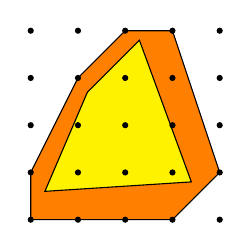
\begin{tikzpicture}[scale=0.6]
	\filldraw[fill=orange] (0,0) -- (0,1) -- (1,3) -- (2,4) -- (3,4) -- (4,1) -- (3,0) --cycle;
	\filldraw[fill=yellow] (0.3,0.6) -- (3.4,0.8) -- (2.3,3.8) --(1.2,2.7) -- cycle;
	\foreach \x in {0,...,4}
	\foreach \y in {0,...,4}
	{
		\filldraw[fill=black] (\x,\y)  circle (1.5pt);
	} 
	% \draw (1,0) -- (0,1) -- (2,2) --cycle;
	\end{tikzpicture}
\end{center} 

This approach is still possible. It is requested by the option 
\begin{itemize}
\itemtt [Approximate, -r]
\end{itemize}

This is often a good choice, especially in low dimension.

It is not advisable to use approximation for polytopes with a large number of vertices since it must be expected that the approximation multiplies the number of vertices by $\dim P+1$ so that it may become difficult to compute the triangulation.

\subsubsection{Lattice points by the dual algorithm}

Often the dual algorithm is extremely fast. But it can also degenerate terribly. It is very fast for \verb|6x6.in| run with \verb|-d1|. The primal algorithm or approximation fail miserably.  (\verb|-1|, the default choice project-and-lift, is also quite good. The difference is that \verb|-d1| does not compute the vertices that in this case are necessary for the preparation of project-and-lift.)

On the other hand, the dual algorithm is hopeless already for the $2$-dimensional parallelotope \verb|ChF_2_64.in|. Try it. It is clear that its complicated arithmetic is forbidding for the dual algorithm. (The dual algorithm successively computes the lattice points correctly for all intermediate polyhedra, defined as intersections of the half spaces that have been processed so far. The intermediate polyhedra can be much more difficult than the final polytope, as in this case.)

In certain cases (see Section \ref{div_labor}) Normaliz will try the dual algorithm if you forbid project-and-lift by \verb|NoProjection|.

\subsubsection{Counting lattice points}\label{Counting}

In some applications one is not interested in the lattice points, but only in their number. In this case you can set the computation goal
\begin{itemize}
	\itemtt [NumberLatticePoints]
\end{itemize}
The main advantage is that it does not store the lattice points and therefore cannot fail because of lack of memory if their number becomes very large. In the inhomogeneous case \verb|NumberLatticePOints| xan be combined with \verb|HilbertSeries|. Then the lattice points are counted by degree. See \ref{count} for an application.

\verb|NumberLatticePoints| uses project-and-lift (with floating point if \verb|ProjectionFloat| is set). Therefore don't block it. If the number of lattice points is so large that memory becomes a problem, then the primal and the dual algorithm will most liokely not be able to compute them.

\subsection{The bottom decomposition}\label{bottom_dec}

The triangulation size and the determinant sum of the triangulation are critical size parameters in Normaliz computations. Normaliz always tries to order the generators in such a way that the determinant sum is close to the minimum, and on the whole this works out well. The use of the bottom decomposition by \verb|BottomDecomposition, -b| enables Normaliz to compute a triangulation with the optimal determinant sum for the given set of generators, as we will explain in the following. 

The determinant sum is independent of the order of the generators of the cone $C$ if they lie in a hyperplane $H$. Then the determinant sum is exactly the normalized volume of the polytope spanned by $0$ and $C\cap H$. The triangulation itself depends on the order, but the determinant sum is constant.
\begin{center}
	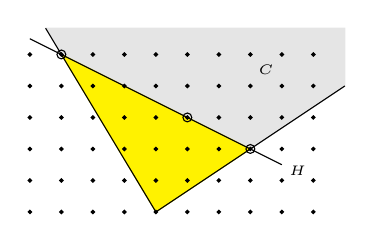
\begin{tikzpicture}[scale=0.4]
	\filldraw[gray!20] (-3.5,5.833) -- (0,0) -- (6,4) -- (6,5.833) -- cycle;
	\filldraw[yellow] (0,0) -- (-3,5) -- (3,2) -- cycle;
	\draw (-3.5,5.833) -- (0,0) -- (6,4);
	\foreach \x in {-4,...,5}
	\foreach \y in {0,...,5}
	{
		\filldraw[fill=black] (\x,\y)  circle (1.5pt);
	}
	\draw (-4,5.5) --(4,1.5) node at (4.5,1.3){\tiny $H$};
	
	\draw (-3,5) circle (4pt) node at (3.5,4.5){\tiny $C$};
	\draw (1,3) circle (4pt);
	\draw (3,2) circle (4pt); 
	\end{tikzpicture}
\end{center}

This observation helps to find a triangulation with minimal determinant sum in the general case.
We look at the \emph{bottom} (the union of the compact faces) of the polyhedron generated by $x_1,\dots,x_n$ as vertices and $C$ as recession cone, and take the volume underneath the bottom: 
\begin{center}
	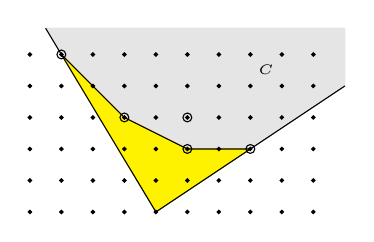
\begin{tikzpicture}[scale=0.4]
	\filldraw[gray!20] (-3.5,5.833) -- (0,0) -- (6,4) -- (6,5.833) -- cycle;
	\filldraw[yellow] (0,0) -- (-3,5) -- (-1,3) -- (1,2) -- (3,2) -- cycle;
	
	\draw (-3,5) -- (-1,3) -- (1,2) -- (3,2);
	
	\draw (-3.5,5.833) -- (0,0) -- (6,4);
	\foreach \x in {-4,...,5}
	\foreach \y in {0,...,5}
	{
		\filldraw[fill=black] (\x,\y)  circle (1.5pt);
	}
	
	\draw (-3,5) circle (4pt) node at (3.5,4.5){\tiny $C$};
	\draw (-1,3) circle (4pt);
	\draw (1,3) circle (4pt);
	\draw (3,2) circle (4pt);
	\draw (1,2) circle (4pt);  
	\end{tikzpicture}
\end{center}
With the option \texttt{BottomDecomposition}, \texttt{-b}, Normaliz computes a triangulation that respects the bottom facets. This yields the optimal determinant sum for the given generators. If one can compute the Hilbert basis by the dual algorithm, it can be used as input, and then one obtains the absolute bottom of the cone, namely the compact facets of the convex hull of all nonzero lattice points. 

Normaliz does not always use the bottom decomposition by default since its computation requires some time and administrative overhead. However, as soon as the input ``profile'' is considered to be ``rough'' it is invoked. The measure of roughness is the ratio between the maximum degree (or $L_1$ norm without a grading) and the minimum. A ratio $\ge 10$ activates the bottom decomposition. 

If you have the impression that the bottom decomposition slows down your computation, you can suppress it by \texttt{NoBottomDec}, \texttt{-o}.

The bottom decomposition is part of the subdivision of large simplicial cones discussed in the next section.

The example \verb|strictBorda.in| belongs to social choice theory like \verb|Condorcet.in| (see Section \ref{Condorcet}), \verb|PluralityVsCutoff.in| and \verb|CondEffPlur.in|. The last two profit enormously from symmetrization (see Section \ref{symmetrize}), but \verb| strictBorda.in| does not. Therefore we must compute the Hilbert series for a monoid in dimension $24$ whose cone has $6363$ extreme rays. It demonstrates the substantial gain that can be reached by bottom decomposition. Since the roughness is large enough, Normaliz chooses bottom decomposition automatically, unless we block it. 
\begin{center}
	\begin{tabular}{|c|r|r|}\hline
		algorithm	& triangulation size& determinant sum \\ \hline
		bottom decomposition& 30,399,162,846 &75,933,588,203 \\ \hline
		standard order of extreme rays,  \ttt{-o} & 119,787,935,829 & 401,249,361,966\\ \hline
	\end{tabular}
\end{center}

\subsection{Subdivision of large simplicial cones}\label{subdiv}

Especially in computations with rational polytopes one encounters very large determinants that can keep the Normaliz primal algorithm from terminating in reasonable time. As an example we take \verb|hickerson-18.in| from the LattE distribution \cite{LatInt}. It is simplicial and the complexity is totally determined by the large determinant $\approx 4.17\times 10^{14}$ (computed with \verb|-v|). 

If we are just interested in the degree $1$ points, Normaliz uses the project-and-lift method of Section \ref{project} and finds $44$ degree $1$ points in the blink of an eye. If we use these points together with the extreme rays of the simplicial cone, then the determinant sum decreases to $\approx 1.3\times 10^{12}$, and the computation of the Hilbert basis and the Hilbert series is in reach. But it is better to pursue the idea of subdividing large simplicial cones systematically. Normaliz employs two methods:
\begin{arab}
\item computation of subdivision points by the IP solver SCIP,
\item its own algorithm for finding optimal subdivision points, based on project-and-lift(and LLL reduced coordinates)
\end{arab}

Normaliz tries to subdivide a simplicial cone if it has determinant $\ge 10^8$ or $10^7$ if the Hilbert basis is computed. Both methods are used recursively via stellar subdivision until simplicial cones with determinant $< 10^6$ have been reached or no further improvement is possible. All subdivision points are then collected, and the start simplicial cone is subdivided with bottom decomposition, which in general leads to substantial further improvement.

The use of SCIP requires a Normaliz executable built with SCIP see Section \ref{Compile}). Moreover, the option \verb|SCIP| must be set since in many cases the Normaliz method is faster and always finds a subdivision point if such exists. 

The following table contains some performance data for subdivisions based on the Normaliz method (default mode, parallelization with 8 threads).
\begin{center}
\setlength{\tabcolsep}{3.2pt}
\renewcommand{\arraystretch}{1.2}
\begin{tabular}{|c|c|c|c|}
\hline
& \ttt{hickerson-16} & \ttt{hickerson-18} & \ttt{knapsack\_11\_60}  \\ \hline
simplex volume & $9.83\times 10^7$ & $4.17\times 10^{14}$ & $2.8\times 10^{14}$ \\ \hline
stellar determinant sum & $3.93\times 10^6$  & $9.07\times 10^8$  & $1.15\times 10^8$\\ \hline
volume under bottom  & $8.10\times 10^5$ & $3.86\times 10^7$ & $2.02\times 10^7$ \\ \hline 
volume used     & $3.93\times 10^6$ & $6.56\times 10^7$ & $2.61\times 10^7$ \\ \hline
%improvement factor & 25 &  $7.62\times10^6$ & $1.17\times 10^7$\\ \hline
runtime without subdivision   &  2.8 s & >12 d &  >8 d \\ \hline
runtime with subdivision    &  0.4 s & 24 s & 5.1 s \\ \hline
\end{tabular}
\end{center}

A good nonsimplicial example showing the subdivision at work is \verb|hickerson-18plus1.in| with option \verb|-q|.

Note: After subdivision the decomposition of the cone may no longer be a triangulation in the strict sense, but a decomposition that we call a \emph{nested triangulation}; see \ref{nested}. If the creation of a nested triangulation must be blocked, one uses the option \verb|NoSubdivision|. Inevitably it blocks the subdivision of large simplicial cones.

\emph{Remark}\enspace The bounds mentioned above work well up to dimension $\approx 10$. For a fixed determinant, the probability for finding a subdivision point decreases rapidly.

\subsection{Primal vs. dual -- division of labor}\label{div_labor}

%\subsection{Normaliz tries to be smart}\label{smart}

As already mentioned several times, Normaliz has two main algorithms for the computation of Hilbert bases and degree $1$ points, the primal algorithm and the dual algorithm. It is in general very hard to decide beforehand which of the two is better for a specific example. Nevertheless Normaliz ties to guess, unless \verb|PrimalMode|, \verb|-P| or \verb|DualMode|, \verb|-d| is explicitly chosen by the user. In first approximation one can day that the dual algorithm is chosen if the computation is based on constraints and the number of inequalities is neither too small nor too large. Normaliz chooses the dual algorithm if at the start of the Hilbert basis computation the cone is defined by $s$ inequalities such that
$$
r+\frac{50}{r} \le s \le 2e
$$
where $r$ is the rank of the monoid to be computed and $e$ is the dimension of the space in which the data are embedded. These conditions ate typically fulfilled for diophantine systems of equations whose nonnegative solutions are asked for. 
In the case of very few or many hyperplanes Normaliz prefers the primal algorithm. While this combinatorial condition is the only criterion for Normaliz, it depends also on the arithmetic of the example what algorithm is better. At present Normaliz makes no attempt to measure it in some way.

When both Hilbert basis and Hilbert series are to be computed, the best solution can be the combination of both algorithms. We recommend \verb|2equations.in| as a demonstration example which combines the algorithmic variant \verb|DualMode| and the computation goal \verb|HilbertSeries|:
\begin{Verbatim}
amb_space 9
equations 2
1 6 -7 -18 25 -36 6 8 -9
7 -13 15 6 -9 -8 11 12 -2
total_degree
DualMode
HilbertSeries
\end{Verbatim}
As you will see, the subdivision of large simplicial cones is very useful for such computations.

Compare \verb|2equations.in| and \verb|2equations_default.in| for an impression on the relation between the algorithms.

\subsection{Volume by descent in the face lattice}\label{descent}

As discussed above, for Hilbert basis computations it is often better to avoid the triangulation based primal algorithm if the input is in terms of inequalities (and other constraints). The same is true for volume or multiplicity computations. Under the same condition as for the automatic choice of the dual algorithm (see Section \ref{div_labor}), Normaliz chooses a method m for volume computation that is based on descent in the face lattice.

While the descent algorithm is not chosen automatically if the number of inequalities exceeds $2*\dim$, it is often very fast also for larger numbers of inequalities, as long as the number of inequalities is moderate. Typical examples are \verb|lo6.in| and \verb|bo5.in|. In both cases, descent is much faster than triangulation which has size $\approx 5*10^9$ and $\approx 20*10^9$, respectively.

Let us come back to \verb|strictBorda.in|. If we run it with \verb|-c|, the terminal output contains
\begin{Verbatim}
Multiplicity by descent in the face lattice
Polytope is not simple
Descent from dim 24, size 1
Descent from dim 23, size 3
...
Descent from dim 12, size 109351
...
Descent from dim 6, size 752392
...
Descent from dim 3, size 106379
..................................................
Mult 1281727528386311499990911876166511/25940255058441281524973174784000000000
Mult (float) 4.94107527277e-05
Full tree size 20378050380
Number of descent steps 9374850
Determinants computed 901955
Number of faces in descent system 4407824
Multiplicity by descent done
\end{Verbatim}
The computation is done in minutes whereas the triangulation based algorithm takes several hours. The data below the multiplicity give some information on the complexity of the computation. The full tree size indicates the size of a triangulation that could be constructed by the same recursion. (We use a 64 bit integer for this magnitude. It is not difficult to make examples that exceed $2^{64}-1$ so that a wrong number is not excluded.)

The idea is to exploit the formula
$$
\operatorname{mult}(P)=\sum_i \operatorname{ht}_{F_i}(v)\operatorname{mult}(F_i)/\deg(v).
$$
recursively where $v$ is a vertex of the polytope $P$ with as few opposite facets $F_i$ as possible, and $\operatorname{ht}_{F_i}(v)$ is the lattice height of $v$ over $F_i$. This requires building a subset $\mathcal F$ of the face lattice so that for each face $F$ to which the formula is applied all the facets of $F$ are contained in $\mathcal F$. However, if a face is simplicial, its multiplicity is computed by the standard determinantal formula.  The  algorithm is implemented in such a way that all data are collected in the descent and no backtracking is necessary. The RAM usage is essentially determined by the two largest layers.

As said above, this algorithm is often chosen by default. You can force it by
\begin{itemize}
	\itemtt[Descent, -F]
\end{itemize}
and block it by
\begin{itemize}
	\itemtt[NoDescent]
\end{itemize}
Note that \verb|Descent| does \emph{not} imply \verb|Multiplicity| or \verb|Volume|. (We cannot exclude that in the future descent is used also for other computations.)

\subsection{Checking  the Gorenstein property}\label{Gorenstein}

If the Hilbert series has been computed, one can immediately see whether the monoid computed by Normaliz is Gorenstein: this is the case if and only if the numerator is a symmetric polynomial, and Normaliz indicates that (see Section \ref{job_dual}). However, there is a much more efficient way to check the Gorenstein property, which does not even require the existence of a grading: we must test whether the \emph{dual} cone has degree $1$ extreme rays. This amounts to checking the existence of an implicit grading on the dual cone.

This very efficient Gorenstein test is activated by the option \ttt{IsGorenstein}, equivalently \ttt{-G} on the command line. We take \verb|5x5Gorenstein.in|:

\begin{Verbatim}
amb_space 25
equations 11
1 1 1 1 1 -1 -1 -1 -1 -1  0  0  0  0  0  0  0  0  0  0  0  0  0  0  0
...
1 1 1 1 0  0  0  0 -1  0  0  0 -1  0  0  0 -1  0  0  0 -1  0  0  0  0
IsGorenstein
\end{Verbatim}

In the output we see
\begin{Verbatim}
Monoid is Gorenstein 
Generator of interior
1 1 1 1 1 1 1 1 1 1 1 1 1 1 1 1 1 1 1 1 1 1 1 1 1 
\end{Verbatim}

In fact, the Gorenstein property is (also) equivalent to the fact that the interior of our monoid is generated by a single element as an ideal, and this generator is computed if the monoid is Gorenstein. (It defines the grading under which the extreme rays of the dual cone have degree~$1$.)

If the monoid is not Gorenstein, Normaliz will print the corresponding message.

\subsection{Symmetrization}\label{symmetrize}

Under certain conditions one can count lattice points in a cone $C$  by mapping $C$ to a cone $C'$ of lower dimension and then counting each lattice point $y$ in $C'$ with the number of its lattice preimages. This approach works well if the number of preimages is given by a polynomial in the coordinates of $y$. Since $C'$ has lower dimension, one can hope that its combinatorial structure is much simpler that that of $C$. One must of course pay a price: instead of counting each lattice point with the weight $1$, one must count it with a polynomial weight. This amounts to a computation of a weighted Ehrhart series that we will discuss in Section \ref{Poly_comp}. Similarly multiplicity can be computed as the virtual multiplicity of a polynomial after projection.

The availability of this approach depends on symmetries in the coordinates of $C$, and therefore we call it \emph{symmetrization}. Normaliz tries symmetrization under the following condition: $C$ is given by constraints (inequalities, equations, congruences, excluded faces) and the inequalities contain the sign conditions $x_i\ge 0$ for all coordinates  $x_i$ of $C$. (Coordinate hyperplanes may be among the excluded faces.) Then Normaliz groups coordinates that appear in all constraints and the grading (!) with the same coefficients, and, roughly speaking, replaces them by their sum. The number of preimages that one must count for the vector $y$  of sums is then a product of binomial coefficients -- a polynomial as desired. More precisely, if $y_j$, $j=1,\dots,m$, is the sum of  $u_j$ variables $x_i$ then
$$
f(y)=\binom{u_1+y_1-1}{u_1-1}\cdots \binom{u_m+y_m-1}{u_m-1}.
$$
is the number of preimages of $(y_1,\dots,y_m)$. This approach to Hilbert series has been suggested by A. Sch\"urmann \cite{Sch}.

As an example we look again at the input for the Condorcet paradox:
\begin{Verbatim}
amb_space 24
inequalities 3
1 1 1 1 1 1 -1 -1 -1 -1 -1 -1   1  1 -1 -1  1 -1   1  1 -1 -1  1 -1
1 1 1 1 1 1  1  1 -1 -1  1 -1  -1 -1 -1 -1 -1 -1   1  1  1 -1 -1 -1
1 1 1 1 1 1  1  1  1 -1 -1 -1   1  1  1 -1 -1 -1  -1 -1 -1 -1 -1 -1
nonnegative
total_degree
Multiplicity
\end{Verbatim}
The grading is completely symmetric, and it is immediately clear that the input is symmetric in the first $6$ coordinates. But also the column of three entries $-1$ appears $6$ times, and there are $6$ more groups of $2$ coordinates each (one group for each $\pm1$ pattern). With the suitable labeling, the number of preimages of$(y_1,\dots,y_8$) is given by
$$
f(y)=\binom{y_1+5}{5}(y_2+1)(y_3+1)(y_4+1)(y_5+1)(y_6+1)(y_7+1)\binom{y_8+5}{5}.
$$
Normaliz finds the groups of variables that appear with the same sign pattern, creates the data for the weighted Ehrhart series, and interprets it as the Hilbert series of the monoid defined by the input data. 

However, there is a restriction. Since the polynomial arithmetic has its own complexity and  Normaliz must do  it in GMP integers, it makes no sense to apply symmetrization if the dimension does not drop by a reasonable amount. Therefore we require that
$$
\dim C' \le \frac{2}{3}\dim C).
$$
If called with the option \verb|-q|,  Normaliz will try symmetrization, and also with \verb|-v|, provoded the multiplicity has not already been computed by the descent algorithm (see Section \ref{descent}). If the inequality for $\dim C'$ is not satisfied, it will simply compute the Hilbert series or the multiplicity without symmetrization. (In default mode it of course tries symmetrization for the Hilbert series.)

Whenever Normaliz has used symmetrization, it writes the file \verb|<project>.symm.out| that contains the data of the symmetrized object. In it you find the multiplicity of \verb|<project>.out| as virtual multiplicity and the Hilbert series as weighted Ehrhart series.

If you use the option \verb|Symmetrize|, then the behavior depends on the other options:
\begin{arab}
\item If neither the \verb|HilbertSeries| nor \verb|Multiplicity| is to be computed, Normaliz writes only the output file \verb|<project>.symm.out| computed with \verb|SupportHyperplanes|.
\item If one of these goals is to be computed, Normaliz will do the symmetrization, regardless of the dimension inequality above (and often this makes sense).
\end{arab}
By doing step (1) first, the user gets useful information of what to expect by symmetrization. In a second run, one can add \verb|HilbertSeries| or \verb|Multiplicity| if (1) was satisfactory.

The Condorcet example is too small in order to demonstrate the power of symmetrization. A suitable example is \verb|PluralityVsCutoff.in|:
\begin{Verbatim}
winfried@ubuntu:~/Dropbox/git_normaliz/source$ time ./normaliz -c ../example/PluralityVsCutoff
                                                    \.....|
                    Normaliz 3.3.0                   \....|
                                                      \...|
     (C) The Normaliz Team, University of Osnabrueck   \..|
                     March  2017                        \.|
                                                         \|
************************************************************
Command line: -c ../example/PluralityVsCutoff 
Compute: DefaultMode 
Embedding dimension of symmetrized cone = 6
...
------------------------------------------------------------
transforming data... done.

real	0m2.655s
user	0m5.328s
sys	0m0.080s
\end{Verbatim}
The Hilbert series is computable without symmetrization, but you better make sure that there is no power failure for the next week if you try that. (The time above includes the Hilbert basis computed automatically in dual mode).

Another good example included in the distribution is \verb|CondEffPlur.in|, but it takes some hours with symmetrization (instead of days without). For it, the dimension drops only from $24$ to $13$.

Symmetrization is a special type of computations with a polynomial weight, and therefore requires Normaliz to be built with CoCoALib. 

\subsection{Computations with a polynomial weight}\label{Poly_comp}

For a graded monoid $M$, which arises as the intersection $M=C\cap L$ of a rational cone$C$  and a lattice $L$,  Normaliz computes the volume of
the rational polytope
$$
P=\{x\in \RR_+ M: \deg x=1\},
$$
called the multiplicity of $M$ (for the given grading), the  Hilbert series of $M$, and the quasipolynomial representing the Hilbert function. This Hilbert series of $M$ is also called the Ehrhart series of $P$ (with respect to $L$), and for the generalization introduced in this section we speak of Ehrhart series and functions.

The computations of these data can be understood as integrals of the
constant polynomial $f=1$, namely with respect to the counting
measure defined by $L$ for the Ehrhart function, and with
respect to the (suitably normed) Lebesgue measure for the
volume. Normaliz generalizes these computations to
arbitrary polynomials $f$ in $n$ variables with rational
coefficients. (Mathematically, there is no need to restrict
oneself to rational coefficients for $f$.)

More precisely, set
$$
E(f,k)=\sum_{x\in M, \deg x=k} f(x),
$$
and call $E(f,\_)$ the \emph{weighted Ehrhart function} for
$f$. (With $f=1$ we simply count lattice points.) The
\emph{weighted Ehrhart series} is the ordinary generating
function
$$
E_f(t)=\sum_{k=0}^\infty E(f,k)t^k.
$$
It turns out that $E_f(t)$ is the power series expansion of a
rational function at the origin, and can always be written in
the form
$$
E_f(t)=\frac{Q(t)}{(1-t^\ell)^{\totdeg f+\rank M}},\qquad Q(t)\in\QQ[t],\
\deg Q< \totdeg f+\rank M.
$$
Here $\totdeg f$ is the total degree of the polynomial $f$, and
$\ell$ is the least common  multiple of the degrees of the
extreme integral generators of $M$. See \cite{BS} for an
elementary account, references and the algorithm used by Normaliz.

At present, weighted Ehrhart series can only be computed  with homogeneous data. Note that \verb|excluded_faces| is a homogeneous input type. For them the monoid $M$ is replaced by the set
$$
M'=C'\cap L
$$
where $C'=C\setminus \mathcal F$ and $\mathcal F$ is the union of a set of
faces
(not necessarily facets) of $C$. What has been said above about the structure
of the weighted Ehrhart series remains true. We discuss an example below.

It follows from the general theory of rational generating
functions that there exists a quasipolynomial $q(k)$ with
rational coefficients and of degree $\le \totdeg f+\rank M-1$ that
evaluates to $E(f,k)$ for all $k\ge 0$.

Let $m=\totdeg f$ (we use this notation to distinguish the degree of the polynomial from the degree of lattice points) and $f_m$ be the degree $m$ homogeneous
component of $f$. By letting $k$ go to infinity and
approximating $f_m$ by a step function that is constant on the
meshes of $\frac 1kL$ (with respect to a fixed basis), one sees
$$
q^{(j)}_{\totdeg f+\rank M-1}=\int_P f_m\, d\lambda
$$
where $d\lambda$ is the Lebesgue measure that takes value $1$
on a basic mesh of $L\cap \RR M$ in the hyperplane of degree
$1$ elements in $\RR M$. In particular, the \emph{virtual
	leading coefficient} $q^{(j)}_{\totdeg f+\rank M-1}$ is
constant and depends only on $f_m$. If the integral vanishes,
the quasipolynomial $q$ has smaller degree, and the true
leading coefficient need not be constant. Following the
terminology of commutative algebra and algebraic geometry, we
call
$$
(\totdeg f+\rank M-1)!\cdot q_{\totdeg f+\rank M-1}
$$
the \emph{virtual multiplicity} of $M$ and $f$. It is an
integer if $f_m$ has integral coefficients and $P$ is a lattice
polytope.

The input format of polynomials has been discussed in Section \ref{poly_input}.

The terminal output contains a factorization of the polynomial as well as some computation results. From the terminal output you may also recognize that Normaliz first computes the triangulation and the Stanley decomposition and then applies the algorithms for integrals and  weighted Ehrhart series.

\emph{Remarks} \enspace (1) Large computations with many parallel threads may require much memory due to the fact that very long polynomials must be stored. Another reason for large memory usage can be the precomputed triangulation or Stanley decomposition.

(2) You should think about the option \verb|BottomDecomposition|. It will be applied to the symmetrized input. (Under suitable conditions it is applied automatically.)

(3) A priori it is not impossible that Normaliz replaces a given grading $\deg$ by $\deg/g$ where $g$ is the grading denominator. If you want to exclude this possibility, set \verb|NoGradingDenom|.
 

\subsubsection{A weighted Ehrhart series}

We discuss the Condorcet paradox again (and the last time), now starting from the symmetrized form. The file \ttt{Condorcet.symm.in} from the directory
\ttt{example} contains the following:

\begin{Verbatim}
amb_space 8
inequalities 3
1 -1 1 1 1 -1 -1 -1
1 1 -1 1 -1 1 -1 -1
1 1 1 -1 -1 -1 1 -1
nonnegative
total_degree
polynomial
1/120*1/120*(x[1]+5)*(x[1]+4)*(x[1]+3)*(x[1]+2)*(x[1]+1)*(x[2]+1)*
(x[3]+1)*(x[4]+1)*(x[5]+1)*(x[6]+1)*(x[7]+1)*(x[8]+5)*(x[8]+4)*
(x[8]+3)*(x[8]+2)*(x[8]+1);
\end{Verbatim}
We have seen this polynomial in Section \ref{symmetrize} above.


From the Normaliz directory we start the computation by
\begin{Verbatim}
./normaliz -cE example/Condorcet.symm
\end{Verbatim}
We could have used \verb|--WeightedEhrhartSeries| instead of \verb|-E| or put \verb|WeightedEhrhartSeries| into the input file.

The file \ttt{Condorcet.symm.out} we find the information on the weighted Ehrhart series:

\begin{Verbatim}
Weighted Ehrhart series:
1 5 133 363 ... 481 15 6
Common denominator of coefficients: 1
Series denominator with 24 factors:
1: 1  2: 14  4: 9

degree of weighted Ehrhart series as rational function = -25

Weighted Ehrhart series with cyclotomic denominator:
...
\end{Verbatim}
The only piece of data that we haven't seen already is the common denominator of coefficients. But since the polynomial has rational coefficients, we cannot any longer expect that the polynomial in the numerator of the series has integral coefficients. We list them as integers, but must then divide them by the denominator (which is$1$ in thus case since the weighted Ehrhart series is a Hilbert series in disguise). As usual, the representation with a denominator of cyclotomic polynomials follows.

And we have the quasipolynomial as usual:

\begin{Verbatim}
Weighted Ehrhart quasi-polynomial of period 4:
 0:   6939597901822221635907747840000 20899225...000000 ... 56262656
 1:   2034750310223351797008092160000  7092764...648000 ... 56262656
 2:   6933081849299152199775682560000 20892455...168000 ... 56262656
 3:   2034750310223351797008092160000  7092764...648000 ... 56262656
with common denominator: 6939597901822221635907747840000
\end{Verbatim}

The left most column indicates the residue class modulo the period, and the
numbers in line $k$ are the coefficients of the $k$-th polynomial after
division by the common denominator. The list starts with $q_0^{(k)}$ and ends
with (the constant) $q_{23}^{(k)}$.
The interpretation of the remaining data is obvious:

\begin{Verbatim}
Degree of (quasi)polynomial: 23

Expected degree: 23

Virtual multiplicity: 1717/8192
Virtual multiplicity (float) = 0.209594726562
\end{Verbatim}


\subsubsection{Virtual multiplicity}

Instead of the option \verb|-E| (or (\verb|--WeightedEhrhartSeries|) we use \verb|-L| or (\verb|--VirtualMultiplicity|). Then we can extract the virtual multiplicity from the output file.

\subsubsection{An integral}
In their paper \emph{Multiplicities of classical varieties} (Proc. Lond. Math. Soc. (3) 110 (2015), 1033--105) J. Jeffries, J. Monta\~no and M. Varbaro ask
for the computation of the integral
$$
\int\limits_{\substack{[0,1]^m \\ \sum{x}= t}}(x_1\cdots x_{m})^{n-m}\prod_{1\le i<j \le m}(x_j-x_i)^2 \mathrm d{\mu}\
$$
taken over the intersection of the unit cube in $\RR^m$ and the hyperplane of constant coordinate sum $t$. It is supposed that $t\le m \le n$. We compute the integral for $t=2$, $m=4$ and $n=6$.

The polytope is specified in the input file \ttt{j462.in} (partially typeset in 2
columns):

\begin{Verbatim}
amb_space 5          -1 0 0 0 1   
inequalities 8       0 -1 0 0 1   
1 0 0 0 0            0 0 -1 0 1   
0 1 0 0 0            0 0 0 -1 1   
0 0 1 0 0            equations 1  
0 0 0 1 0            -1 -1 -1 -1 2
grading
unit_vector 5
polynomial
(x[1]*x[2]*x[3]*x[4])^2*(x[1]-x[2])^2*(x[1]-x[3])^2*
(x[1]-x[4])^2*(x[2]-x[3])^2*(x[2]-x[4])^2*(x[3]-x[4])^2;
\end{Verbatim}

The $8$ inequalities describe the unit cube in $\RR^4$ by the inequalities  $0\le z_i\le 1$
and the equation gives the hyperplane $z_1+\dots+z_4=2$ (we must use homogenized coordinates!). (Normaliz would find the grading itself.)

From the Normaliz directory the computation is called by

\begin{Verbatim}
./normaliz -cI example/j462
\end{Verbatim}
where \verb|-I| could be replaced by \verb|--Integral|.

It produces the output in \ttt{j462.out} containing

\begin{Verbatim}
integral  = 27773/29515186701000
integral  (float) = 9.40973210888e-10
\end{Verbatim}

As pointed out above, Normaliz integrates with respect to the measure in which the basic lattice mesh has volume $1$. (this is $r!$ times the lattice normalized measure, $r=\dim P$.) In the full.dimensional case that is just the standard Lebesgue measure. But in lower dimensional cases this often not the case, and therefore Normaliz also computes the integral with respect to this \emph{Euclidean} measure:
\begin{Verbatim}
integral (euclidean) = 1.88194642178e-09
\end{Verbatim}

Note that \verb|Integral| automatically sets \verb|NoGradingDenom| since the polytope must be fixed for integrals. 

\subsubsection{Restrictions in MS Windows}

We have not succeeded in compiling Normaliz with CoCoALib under MS Windows. in previous versions of Normaliz, the computations with polynomial weights were done by the separate program NmzIntegrate, and NmzIntegrate can still be used (in all operating systems). One must start the computation from NmzIntegrate (and not from Normaliz, as was also possible in previous versions).

Unfortunately 1.3 is the last version of NmzIntegrate that we could compile under MS Windows. This causes some restrictions in the use of NmzIntegrate:

\begin{arab}
	\item Due to a bug it is possible that a segmentation fault occurs if excluded faces are used. 
	\item The option \verb|OutputDir| is not available.
\end{arab}

An excellent way out is to run Normaliz (and NmzIntegrate) in the Linux subsystem of Windows 10 or in the Docker container.

\subsection{Expansion of the Hilbert or weighted Ehrhart series}\label{expansion}

Normaliz can compute the expansion of the Hilbert function or the weighted Ehrhart function up to a given degree. To this end its expands the series. For the Hilbert function there is a second possibility by lattice point computation.

\subsubsection{Series expansion}
This is best explained by \verb|CondorcetExpansion.in|:
\begin{Verbatim}
amb_space 24
inequalities 3
1 1 1 1 1 1      -1 -1 -1 -1 -1 -1   1 1 -1 -1 1 -1     1 1 -1 -1 1 -1
1 1 1 1 1 1       1 1 -1 -1 1 -1    -1 -1 -1 -1 -1 -1   1 1 1 -1 -1 -1
1 1 1 1 1 1       1 1 1 -1 -1 -1     1 1 1 -1 -1 -1    -1 -1 -1 -1 -1 -1
nonnegative
total_degree
HilbertSeries
expansion_degree 50
\end{Verbatim}
By \verb|expansion_degree 50| we tell Nprmaliz to compute the coefficients from degree $0$ to degree $50$  in theexpansion of the Hilbertt series. So the output contains
\begin{Verbatim}
Expansion of Hilbert series
0: 1
1: 6
2: 153
3: 586
4: 7143
5: 21450
...
49: 817397314032054600
50: 1357391110355875044
\end{Verbatim}
If the shift is nonzero, it is automatically added to the degree so that the expansion always starts at the shift. 

The expansion degree applies to the weighted Ehrhart series as well if it is computed.

There is nothing more to say, except that (in principle) there is another method, as discussed in the next section.

\subsubsection{Counting lattice points by degree}\label{count}

As an example we look at \verb|CondorcetRange.in|:
\begin{Verbatim}
amb_space 24
inequalities 3
1 1 1 1 1 1      -1 -1 -1 -1 -1 -1   1 1 -1 -1 1 -1     1 1 -1 -1 1 -1
1 1 1 1 1 1       1 1 -1 -1 1 -1    -1 -1 -1 -1 -1 -1   1 1 1 -1 -1 -1
1 1 1 1 1 1       1 1 1 -1 -1 -1     1 1 1 -1 -1 -1    -1 -1 -1 -1 -1 -1
nonnegative
total_degree
constraints 2
1 1 1 1 1 1 1 1 1 1 1 1 1 1 1 1 1 1 1 1 1 1 1 1 <= 5
1 1 1 1 1 1 1 1 1 1 1 1 1 1 1 1 1 1 1 1 1 1 1 1 >= 3
Projection
NumberLatticePoints
HilbertSeries
expansion_degree 5
\end{Verbatim}
This input defines the polytope that is cut out from the cone (defined by the $3$ inequalities) by the two inequalities that are defined as constraints (for clarity). These two inequalities mean that we want to compute the polytope of all points $x$ in the cone satisfying the condition $3\le \deg x \le 5$. We add \verb|Projection| in conjunction with \verb|LatticePoints| to keep Normaliz from choosing the primal algorithm, which would do the job as well, but much more slowly.

In the output we find
\begin{Verbatim}
Hilbert series:
586 7143 21450 
denominator with 0 factors:

shift = 3
\end{Verbatim}

Taking the shift into account, we see that there are 586 lattice points in degree $3$, $7413$ in degree $4$ and $21450$ in degree $5$. But this becomes even more obvious by (the unnecessary) \verb|expansion_degree 5|:
\begin{Verbatim}
Expansion of Hilbert series
3: 586
4: 7143
5: 21450
\end{Verbatim}
With \verb|NumberLatticePopints| the lattice points are not stored. Therefore very large numbers of lattice points can be computed.  (But they must be produced, and the production process also needs some space, which however depends only on the dimension.)


\subsection{Significant coefficients of the quasipolynomial}\label{highest_coeff}

If the degree and simultaneously the period of the Hilbert or weighted Ehrhart quasipolynomial are large, the space needed to store it (usually with large coefficients) may exceed the available memory. Depending on the application, only a certain number of the coefficients may be significant. Therefore one can limit the number of highest coefficients that are stored and printed. We look at the input file \texttt{CondorcetN.in}:
\begin{Verbatim}
amb_space 24
inequalities 3
1 1 1 1 1 1     -1 -1 -1 -1 -1 -1     1  1 -1 -1  1 -1     1  1 -1 -1  1 -1
1 1 1 1 1 1      1  1 -1 -1  1 -1    -1 -1 -1 -1 -1 -1     1  1  1 -1 -1 -1
1 1 1 1 1 1      1  1  1 -1 -1 -1     1  1  1 -1 -1 -1    -1 -1 -1 -1 -1 -1
nonnegative
total_degree
nr_coeff_quasipol 2
\end{Verbatim}

The output file shows the following information on the quasipolynomial:
\begin{Verbatim}
Hilbert quasi-polynomial of period 4:
only 2 highest coefficients computed
their common period is 2
0:  0 0 0 0 0 0 0 0 0 0 0 0 0 0 0 0 0 0 0 0 0 0 15982652919 56262656
1:  0 0 0 0 0 0 0 0 0 0 0 0 0 0 0 0 0 0 0 0 0 0 15528493056 56262656
with common denominator = 6939597901822221635907747840000
\end{Verbatim}
Normaliz computes and prints only as many components of the quasipolynomial as required by the common period of the printed coefficients. Coefficients outside the requested range are printed as $0$.

The bound on the significant coefficients applies simultaneously to the Hilbert polynomial and the weighted Ehrhart quasipolynomial---usually one is interested in only one of them.

By default Normaliz computes the quasipolynomial only if the period does not exceed a preset bound, presently $10^6$. If this bound is too small for your computation, you can remove it by the option
\begin{Verbatim}
NoPeriodBound
\end{Verbatim}



\subsection{Explicit dehomogenization}\label{dehom_ex}
Inhomogeneous input for data in $\RR^{d}$ is homogenized by an extra $(d+1)$th coordinate. The dehomogenization sets the last coordinate equal to $1$. Other systems may prefer the first coordinate. By choosing an explicit dehomogenization Normaliz can be adapted to such input. The file \verb|dehomogenization.in|
\begin{Verbatim}
amb_space 3
inequalities 2
-1 1 0
-1 0 1
dehomogenization
unit_vector 1
\end{Verbatim}
indicates that in this case the first variable is the homogenizing one. The output file
\begin{Verbatim}
1 module generators
2 Hilbert basis elements of recession monoid
1 vertices of polyhedron
2 extreme rays of recession cone
3 support hyperplanes of polyhedron (homogenized)

embedding dimension = 3
affine dimension of the polyhedron = 2 (maximal)
rank of recession monoid = 2

size of triangulation   = 0
resulting sum of |det|s = 0

dehomogenization:
1 0 0 


module rank = 1

***********************************************************************

1 module generators:
1 1 1

2 Hilbert basis elements of recession monoid:
0 0 1
0 1 0

1 vertices of polyhedron:               3 support hyperplanes of polyhedron (homogenized)
1 1 1                                   -1 0 1
                                        -1 1 0
2 extreme rays of recession cone:        1 0 0
0 0 1
0 1 0
\end{Verbatim}
shows that Normaliz does the computation in the same way as with implicit dehomogenization, except that now the first coordinate decides what is in the polyhedron and what belongs to the recession cone, roughly speaking.

Note that the dehomogenization need not be a coordinate. It can be any linear form that is nonnegative on the cone generators.

\subsection{Projection of cones and polyhedra}\label{Proj_cone}

Normaliz can not only compute projections (as has become visible in the discussion of project-and-float), but also export them if asked for by the computation goal
\begin{itemize}
	\itemtt[ProjectCone]
\end{itemize}
As the computation goal says, only the cone is projected. Lattice data are not taken care of. The image of the projection is computed with the goals \verb|SupportHyperplanes| and \verb|ExtremeRays|, and the result is contained in an extra output file \verb|<project>.ProjectCone.out|, similarly to the result of the integer hull computation. (All other computation goals are applied to the input cone.)

The image and the kernel a of the projection are complementary  vector subspaces generated by unit vectors. Those spanning the image are selected by the entries $1$ in the $0$-$1$ vector \verb|projection_coordinates| of the input file. As an example we take
\verb|small_proj.in|:
\begin{Verbatim}
amb_space 6
cone 190
6 0 7 0 10 1
...
0 0 0 16 7 1
projection_coordinates
1 1 0 1 0  1
ProjectCone
\end{Verbatim}
As you can see from \verb|small_proj.out|, almost nothing is computed dor the input cone itself. (However, any further computation goal would change this.) The result of the projection is contained in \verb|small_proj.ProjectCone.out|:
\begin{Verbatim}
14 extreme rays
9 support hyperplanes

embedding dimension = 4
...
14 extreme rays:
0  0  1 1
0  0 17 1
 ...
 11  0  5 1
 11  0  6 1
 
 9 support hyperplanes:
 -1 -1 -1 20
 ...
  1  0  1 -1
\end{Verbatim}
In this example, the input is of type ``generators''. Normaliz simply projects them and uses the images as input of type \verb|cone| for the projection. If the input is of type ``constraints'', as in \verb|small_sh_proj.in|, 
\begin{Verbatim}
amb_space 6
inequalities 32
 0 -2 -2  0 -1 24
-1 -1 -1 -1 -1 23
...
 -2 -1  0  1 -1 28
  0  1  1 -1  0 16
 projection_coordinates
 1 1 0 1 0  1
 ProjectCone
\end{Verbatim}
then Normaliz uses the projection part of the project-and-lift algorithm to find the result, as you can see from the terminal output. Equivalent inhomogeneous input files are \verb|small_proj_inhom.in| and \verb|small_sh_proj_inhom.in|.

Polyhedra and polytopes are treated by Normaliz as intersections of cones and hyperplanes. The hyperplane is given by the grading in the homogeneous case and by the dehomogenization in the inhomogeneous case. For the projection of the polyhedron, the kernel of the projection must be parallel to this hyperplane. Normaliz checks this condition (automatically satisfied for inhomogeneous input) and transfers the grading or the dehomogenization, respectively, to the image. Therefore the image of the input polyhedron is indeed the polyhedron defined by the projection.

\subsection{Nonpointed cones}\label{Nonpointed}

Nonpointed cones and nonpositive monoids contain nontrivial invertible elements. The main effect is that certain data are no longer unique, or may even require a new definition. An important point to note is that cones always split off their unit groups as direct summands and the same holds for normal affine monoids. Since Normaliz computes only normal affine monoids, we can always pass to the quotient by the unit groups. Roughly speaking, all data are computed for the pointed quotient and then lifted back to the original cone and monoid. It is inevitable that some data are no longer uniquely determined, but are unique only modulo the unit group, for example the Hilbert basis and the extreme rays. Also the multiplicity and the Hilbert series are computed for the pointed quotient. From the algebraic viewpoint this means to replace the field $K$ of coefficients by the group ring $L$ of the unit group, which is a Laurent polynomial ring over $K$: instead of $K$-vector space dimensions one considers ranks over $L$.

\subsubsection{A nonpointed cone}

As a very simple example we consider the right halfplane (\verb|halfspace2.in|):
\begin{Verbatim}
amb_space 2
inequalities 1 
1 0
\end{Verbatim}
When run in default mode, it yields the following output:
\begin{Verbatim}
1 Hilbert basis elements
1lattice points in polytope (Hilbert basis elements of degree 1)
1 extreme rays
1 support hyperplanes

embedding dimension = 2
rank = 2 (maximal)
external index = 1
dimension of maximal subspace = 1

size of triangulation   = 1
resulting sum of |det|s = 1

grading:
1 0 

degrees of extreme rays:
1: 1  

Hilbert basis elements are of degree 1

multiplicity = 1

Hilbert series:
1 
denominator with 1 factors:
1: 1  

degree of Hilbert Series as rational function = -1

Hilbert polynomial:
1 
with common denominator = 1

rank of class group = 0
class group is free

***********************************************************************

1 lattice points in polytope (Hilbert basis elements of degree 1):
1 0

0 further Hilbert basis elements of higher degree:

1 extreme rays:
1 0

1 basis elements of maximal subspace:
0 1

1 support hyperplanes:
1 0
\end{Verbatim}

In the preamble we learn that the cone contains a nontrivial subspace. In this case it is the vertical axis, and close to the end we see a basis of this subspace, namely $(0,1)$. This basis is always simultaneously a $\ZZ$-basis of the unit group of the monoid. The rest of the output is what we have gotten for the positive horizontal axis which in this case is a natural representative of the quotient modulo the maximal subspace, The quotient can always be embedded in the cone or monoid respectively, but there is no canonical choice. We could have gotten $(1,5)$ as the Hilbert basis as well.

Normaliz has found a grading. Of course it vanishes on the unit group, but is positive on the quotient monoid modulo the unit group.

Note that the data of type ``dimension'' (embedding dimension, rank, rank of recession monoid in the inhomogeneous case, affine dimension of the polyhedron)) are measured before the passage to the quotient modulo the maximal subspace. The same is true for equations and congruences (which are trivial for the example above).

\subsubsection{A polyhedron without vertices}

We define the affine halfspace of the figure by \verb|gen_inhom_nonpointed.in|:
\begin{Verbatim}
amb_space 2
cone 3
1 -1
-1 1
0 1
vertices 1
-1 -1 3
\end{Verbatim}

\begin{center}
	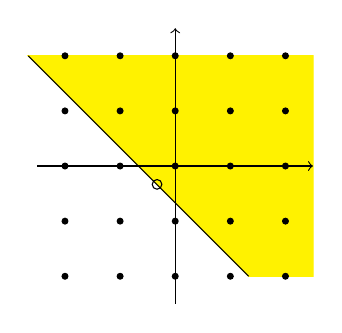
\begin{tikzpicture}[scale=0.7]
	
	\filldraw[yellow] (1.333,-2) -- (-2.667,2) -- (2.5,2) -- (2.5,-2) -- cycle;
	
	\foreach \x in {-2,...,2}
	\foreach \y in {-2,...,2}
	{
		\filldraw[fill=black] (\x,\y)  circle (1.5pt);
	}
	\draw[->] (-2.5,0) -- (2.5,0);
	\draw[->] (0,-2.5) -- (0,2.5);
	\draw (1.333,-2) -- (-2.667,2);
	\draw (-0.33,-0.333)  circle (2.5pt); 
	\end{tikzpicture}
\end{center}

It is clear that the ``vertex'' is not a vertex in the strict sense, bt only gives a displacement of the cone. The output when run in default mode:

\begin{Verbatim}
1 module generators
1 Hilbert basis elements of recession monoid
1 vertices of polyhedron
1 extreme rays of recession cone
2 support hyperplanes of polyhedron (homogenized)

embedding dimension = 3
affine dimension of the polyhedron = 2 (maximal)
rank of recession monoid = 2
internal index = 3
dimension of maximal subspace = 1

size of triangulation   = 1
resulting sum of |det|s = 3

dehomogenization:
0 0 1 


module rank = 1

***********************************************************************

1 module generators:
0 0 1

1 Hilbert basis elements of recession monoid:
0 1 0

1 vertices of polyhedron:
0 -2 3

1 extreme rays of recession cone:
0 1 0

1 basis elements of maximal subspace:
1 -1 0

2 support hyperplanes of polyhedron (homogenized):
0 0 1
3 3 2
\end{Verbatim}

The ``vertex'' of the polyhedron shown is of course the lifted version of the vertex modulo the maximal subspace. It is not the input ``vertex'', but agrees with it up to a unit.

\subsubsection{Checking pointedness first}\label{IsPointed}

Nonpointed cones will be an exception in Normaliz computations, and therefore Normaliz assumes that the (recession) cone it must compute is pointed. Only in rare circumstances it could be advisable to have this property checked first. There is no need to do so when the dual algorithm is used since it does not require the cone to be pointed. Moreover, if an explicit grading is given or a grading dependent computation is asked for, one cannot save time by checking the pointedness first.

The exceptional case is a computation, say of a Hilbert basis, by the primal algorithm in which the computation of the support hyperplanes needs very long time to be completed. If you are afraid this may happen, you can force Normaliz to compute the support hyperplanes right away by adding \verb|IsPointed| to the computation goals. This is a disadvantage only if the cone is unexpectedly pointed.

\subsubsection{Input of a subspace} \label{subspace}

If a linear subspace contained in the cone is known a priori, it can be given to Normaliz via the input type \verb|subspace|. If Normaliz detects a \verb|subspace|, it appends the rows of the matrix to the generators of the cone, and additionally the negative of the sum of the rows (since we must add the subspace as a cone). If \verb|subspace| is combined with \verb|cone_and_lattice|, then the rows of \verb|subspace| are also appended to the generators of the lattice. It is not assumed that the vectors in \verb|subspace| are linearly independent or generate the maximal linear subspace of the cone. A simple example (\verb|subspace4.in|):
\begin{Verbatim}
amb_space 4
cone 4
1 0 2 0
0 1 -2 1
0 0 0 1
0 0 0 -1
subspace 1
0 0 1 0
\end{Verbatim}

From the output:
\begin{Verbatim}
2 lattice points in polytope (Hilbert basis elements of degree 1):
 0 1 0 0
 1 0 0 0

0 further Hilbert basis elements of higher degree:

2 extreme rays:
 0 1 0 0
 1 0 0 0

2 basis elements of maximal subspace:
 0 0 1 0
 0 0 0 1

2 support hyperplanes:
 0 1 0 0
 1 0 0 0
\end{Verbatim}
 
One should note that the maximal subspace is generated by the smallest face that contains all invertible elements. Therefore, in order to make all vectors in a face invertible, it is enough to put a single vector from the interior of the face into \verb|subspace|.
 
\subsubsection{Data relative to the original monoid}

If original monoid generators are defined, there are two data related to them that must be read with care.

First of all, we consider the original monoid generators as being built from the vectors in \verb|cone| or \verb|cone_and_lattice| plus the vectors in \verb|subspace| and additionally the negative of the sum of the latter (as pointed out above). 

The test for ``Original monoid is integrally closed' is correct -- it returns \verb|true| if and only if the original monoid as just defined indeed equals the computed integral closure. (There was a mistake in version 3.0.)

The ``module generators over the original monoid'' only refer to the \emph{image} of the original monoid and the image of the integral closure \emph{modulo the maximal subspace}. They do not take into account that the unit group of the integral closure may not be generated by the original generators. An example in which the lack of integral closedness is located in the unit group (\verb|normface.in|):

\begin{Verbatim}
amb_space 5
cone 4
0 0 0 1 1
1 0 0 1 1
0 1 0 1 1
0 0 1 1 1
subspace 4
0 0 0 0 1
1 0 0 0 1
0 1 0 0 1
1 1 2 0 1
\end{Verbatim}

From the output file:

\begin{Verbatim}
...
dimension of maximal subspace = 4
original monoid is not integrally closed
unit group index = 2
...

1 lattice points in polytope (Hilbert basis elements of degree 1):
0 0 0 1 0
...
1 module generators over original monoid:
0 0 0 0 0
\end{Verbatim}
The original monoid is not integrally closed since the unit group of the integral closure is strictly larger than that of the original monoid: the extension has index $2$, as indicated. The quotients modulo the unit groups are equal, as can be seen from the generator over the original monoid or the Hilbert basis (of the integral closure) that is contained in the original monoid.


\subsection{Exporting the triangulation}\label{Triang}

The option \ttt{-T} asks Normaliz to export the triangulation by writing the files 
 \ttt{<project>.tgn} and \verb|<project>.tri|:

\begin{itemize}
	
	\itemtt[tgn]     The file \ttt{tgn} contains a matrix of vectors (in the
	coordinates of $\AA$) spanning the simplicial cones in
	the triangulation.
	
	\itemtt[tri]
	The file \ttt{tri} lists the simplicial subcones. There are two variants, depending on whether \verb|ConeDecomposition| had been set. Here we assume that \verb|ConeDecomposition| is not computed. See Section \ref{Disjoint} for the variant with \verb|ConeDecomposition|.
	
	The first line contains the number of simplicial cones
	in the triangulation, and the next line contains the
	number $m+1$ where $m=\rank \EE$. Each of the following
	lines specifies a simplicial cone $\Delta$: the first
	$m$ numbers are the indices (with respect to the order
	in the file \ttt{tgn}) of those generators that span
	$\Delta$, and the last entry is the multiplicity of
	$\Delta$ in $\EE$, i.~e.\ the absolute value of the
	determinant of the matrix of the spanning vectors (as
	elements of $\EE$).
\end{itemize}

The following example is the $2$-dimensional cross polytope with one excluded face (\verb|cross2.in|). The excluded face is irrelevant for the triangulation.

\begin{Verbatim}
amb_space 3
polytope 4                           
1  0                      
0  1                
-1  0
0 -1
excluded_faces 1
1  1 -1                         
\end{Verbatim}

Its \verb|tgn| and \verb|tri| files are
\begin{Verbatim}
tgn             tri
4               2
3               4
1 0 1           1 2 3    2
0 1 1           1 3 4    2
-1 0 1          plain
0 -1 1                 
\end{Verbatim}

We see the $4$ vertices $v_1,\dots,v_4$ in homogenized coordinates in \verb|tgn| and the $2$ simplices (or the simplicial cones over them) in \verb|tri|: both have multiplicity $2$. The last word \verb|plain| indicates that Normaliz has computed a triangulation in the strict sense, namely a simplicial subdivision in which neighboring simplicial cones match along common faces. The alternative is \verb|nested| that we discuss below.

In addition to the files \verb|<project>.tgn| and \verb|<project>.tri|, also the file \verb|<object>.inv| is written. It contains the data of the file \verb|<project>.out| above the line of stars in a human and machine readable format.

\subsubsection{Nested triangulations}\label{nested}

If Normaliz has subdivided a simplicial cone of a triangulation of the cone $C$, the resulting decomposition of $C$ may no longer be a triangulation in the strict sense. It is rather a \emph{nested triangulation}, namely a map from a rooted tree to the set of full-dimensional subcones of $C$ with the following properties:
\begin{arab}
\item the root is mapped to $C$,
\item every other node is mapped to a full dimensional simplicial subcone,
\item the simplicial subcones corresponding to the branches at a node $x$ form a triangulation of the simplicial cone corresponding to $x$.
\end{arab}

The following figure shows a nested triangulation:

\begin{center}
	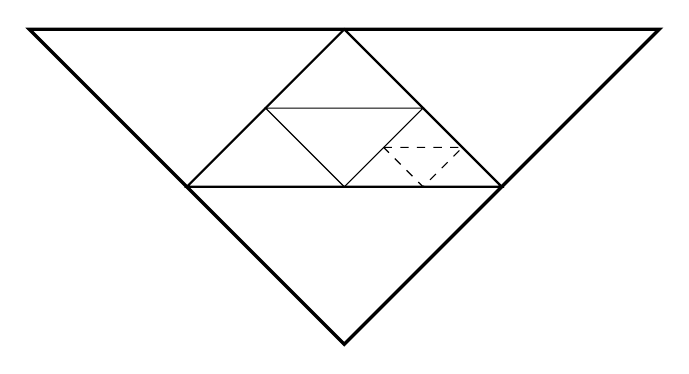
\begin{tikzpicture}[scale=1.0]
	\draw[very thick] (-4,4)  -- (4,4) -- (0,0) -- cycle;
	\draw[thick] (-2,2) -- (2,2) -- (0,4) -- cycle;
	\draw (-1,3) -- (1,3) -- (0,2) -- cycle;
	\draw[dashed] (0.5,2.5) --(1.5,2.5) -- (1.0,2) --cycle;
\end{tikzpicture}
\end{center}

For the Normaliz computations, nested triangulations are as good as ordinary triangulations, but in other applications the difference may matter. With the option \verb|-T|, Normaliz prints the leaves of the nested triangulation to the \verb|tri| file. They constitute the simplicial cones that are finally evaluated by Normaliz.

The triangulation is always plain if \verb|-T| is the only computation goal or if it is just combined with \verb|-v|. Otherwise it can only fail to be plain if it contains determinants $\ge 10^8$.

The subdivision can be blocked by \verb|NoSubdivision|, independently of the computation goals.

\subsubsection{Disjoint decomposition}\label{Disjoint}

Normaliz can export the disjoint decomposition of the cone that it has computed. This decomposition is always computed together with a full triangulation, unless only the multiplicity is asked for. It represents the cone as the disjoint union of semiopen simplicial subcones. The corresponding closed cones constitute the triangulation, and from each of them some facets are removed so that one obtains a disjoint decomposition. See \cite{BIS} for more information. In the following figure, the facets separating the triangles are omitted in the triangle on the $-$ side.

\begin{center}
	\begin{scriptsize}
		%\tikzstyle{every node}=[circle, draw, fill=black, inner sep=0pt, minimum width=3pt]
		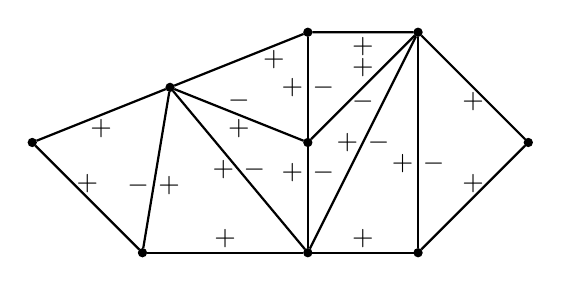
\begin{tikzpicture}
		[scale=0.7,auto=left, thick]
		%\foreach \from/\to in {n2/n4,n2/n5,n4/n5,n4/n6,n5/n7,n6/n7}
		%  \foreach \x in {0, 1, ..., 9}
		\foreach \x/\y in {0/2, 2/0, 5/0, 5/2, 5/4, 7/0, 7/4, 9/2}
		\node [circle, draw, fill=black, inner sep=0pt, minimum width=2.5pt](n\x\y) at (\x,\y) {};
		\node [circle, draw, fill=black, inner sep=0pt, minimum width=2.5pt](n23) at (2.5,3) {};
		%\node [circle, draw, inner sep=0pt, minimum width=3pt, label=above:$O_C$](OC) at (2.8,1.7) {};
		
		%  \draw (\from) -- node[above]{$+$} node[below]{$-$} (\to);
		\draw (n20) -- node[right=-2pt, pos=0.4]{$+$} node[left=-2pt, pos=0.4]{$-$} (n23);
		\draw (n20) -- node[above=-2pt]{$+$} (n02);
		\draw (n50) -- node[right=-2pt]{$-$} node[left=-2pt]{$+$} (n23);
		\draw (n50) -- node[near end, right=-2pt]{$-$} node[near end, left=-2pt]{$+$} (n52);
		\draw (n52) -- node[right=-2pt]{$-$} node[left=-2pt]{$+$} (n54);
		\draw (n70) -- node[right=-2pt, pos=0.4]{$-$} node[left=-2pt, pos=0.4]{$+$} (n74);
		
		\draw (n52) -- node[below=-2pt]{$+$} node[above=-2pt]{$-$} (n23);
		\draw (n52) -- node[below=-2pt]{$-$} node[above]{$+$} (n74);
		\draw (n50) -- node[right=-2pt]{$-$} node[left=-2pt]{$+$} (n74);
		
		\draw (n02) -- node[below=-2pt]{$+$} (n23);
		\draw (n23) -- node[right=5pt]{$+$} (n54);
		\draw (n20) -- node[above=-2pt]{$+$} (n50);
		\draw (n50) -- node[above=-2pt]{$+$} (n70);
		\draw (n54) -- node[below=-2pt]{$+$} (n74);
		\draw (n70) -- node[above=-2pt]{$+$} (n92);
		\draw (n74) -- node[below=-2pt]{$+$} (n92);
		
		
		%  \draw[to] (daq) -- node[midway,right] {raw event data\\level 1} (buffer);
		% \draw[to] (monitor) -- node[midway,above] {events} node[midway,below] {level 1} (datastore);
		\end{tikzpicture}
	\end{scriptsize}
\end{center}

If you want to access the disjoint decomposition, you must activate the computation goal \verb|ConeDecomposition| or use the command line option is \verb|-D|. As an example we compute \verb|cross2.in| with the computation goal \verb|ConeDecomposition|. The file \verb|cross2.tri| now looks as follows:

\begin{Verbatim}
2
7
1 2 3    2    0 0 0
2 3 4    2    0 0 1
plain
\end{Verbatim}

As before the first line contains the size of the triangulation and the second is the number of entries of each row.
The first $3$ entries in each line are the indices of the extreme rays with respect to the \verb|tgn| file and the fourth entry is the determinant. They are followed by a $0/1$ vector indicating the open facets in the order in which they are opposite to the extreme rays. If the corresponding entry is $1$, the facet must be removed. 

In our example all facets of the first simplicial cone are kept, and from the second simplicial cone the facet opposite to the third extreme ray (with index $4$ relative to \verb|tgn|) must be removed.

The disjoint decomposition which is the basis of all Hilbert series computations uses the algorithm suggested by K\"oppe and Verdoolaege \cite{KV}.


\subsection{Exporting the Stanley decomposition}\label{Stanley}

The option \ttt{-y} makes Normaliz 
write the files  \ttt{<project>.tgn}, \verb|<project>.dec| and \verb|<project>.inv|.   Stanley decomposition is contained in the file with the suffix \verb|dec|. But this file also contains the inclusion/exclusion data if there are excluded faces:

(a) If there are any excluded faces, the file starts with the word
\verb|in_ex_data|. The next line contains the number of such data that follow.
Each of these lines contains the data of a face and the coefficient with which
the face is to be counted: the first number lists the number of generators that
are contained in the face, followed by the indices of the generators relative
to the \verb|tgn| file and the last number is the coefficient.

(b) The second block (the first if there are no excluded faces) starts with
the word \verb|Stanley_dec|, followed by the number of simplicial cones in the
triangulation.

For each simplicial cone $\Delta$ in the
triangulation this file contains a block of data:
\begin{enumerate}
	\item[(i)] a line listing the indices $i_1,\dots,i_m$ of the
	generators $v_{i_1},\dots,v_{i_m}$ relative to the
	order in \ttt{tgn} (as in \ttt{tri}, $m=\rank \EE$);
	
	\item[(ii)] a $\mu\times m$ matrix where $\mu$ is the
	multiplicity of $\Delta$ (see above).
	
	In the notation of \cite{BIS}, each line lists an
	``offset'' $x+\epsilon(x)$  by its coordinates with
	respect to $v_{i_1},\dots,v_{i_m}$ as follows: if
	$(a_1,\dots,a_m)$ is the line of the matrix, then
	$$
	x+\epsilon(x)=\frac{1}{\mu}(a_1v_{i_1}+\dots+a_mv_{i_m}).
	$$
\end{enumerate}


The \verb|dec| file of the example above is
\begin{Verbatim}
in_ex_data
1
2 1 2 -1
Stanley_dec
2
1 3 4              1 2 3 
2                  2     
3                  3     
0 0 2              0 0 0 
1 1 2              1 0 1
\end{Verbatim}

There is $1$ face in \verb|in_ex_data| (namely the excluded one), it contains the $2$ generators $v_1$ and $v_2$  and appears with multiplicity $-1$. The Stanley decomposition consists of $4$ components of which each of the simplicial cone contains $2$. The second offset in the second simplicial cone is
$$
\frac12 (1v_1+0v_2+1v_3)=(0,0,1).
$$ 

 We recommend you to process the file \ttt{3x3magiceven.in} with the
option \ttt{-ahTy} activated. Then inspect all
the output files in the subdirectory \ttt{example} of the
distribution.

\subsection{Face lattice and f-vector}\label{FaceLattice}

In connection with ``face'', ``lattice'' means a partially ordered set with meet and join. Every face of a polyhedron is the intersection of the facets that contain it, and therefore Normaliz computes all intersections of facets, including the polyhedron itself and the empty set if the intersection of all facets should be empty.

The computation of the face lattice or just the f-vector might require very much memory. Therefore one should be careful if the dimension is large or there are many support hyperplanes.

The file \verb|rationalFL.in| contains
\begin{Verbatim}
amb_space 3
polytope 3
1/2 1/2
-1/3 -1/3
1/4 -1/2
HilbertSeries
FaceLattice
\end{Verbatim}
representing a rational triangle. (Without \verb|FaceLattice| it has been discussed in Section \ref{rational}.)

Since the face lattice can be very large, it is returned as a separate file \verb|<project>.fac|. For our example we get \verb|rationalFL.fac|:
\begin{Verbatim}
8
3

000 0
100 1
010 1
110 2
001 1
101 2
011 2
111 3
\end{Verbatim}
The first line contains the number of faces, and the second the number of facets. The other lines list the faces $F$, encoded by a a $0$-$1$-vector and an integer. The integer is the codimension of $F$d.  The $0$-$1$-vector lists the facets containing $F$: the entry $1$ at the $i$-the coordinate indicates that the $i$-th facet contains $F$.

The facets are counted as given in the first matrix of the file  \verb|<project>.cst| which is generated as well. In our case \verb|rationalFL.cst| contains
\begin{Verbatim}
3
3
-8 2 3 
1 -1 0 
2 7 3 
inequalities
...
\end{Verbatim}
So, for example, the face \verb|011| is contained in the facets  given by the linear forms $(1,-1,0)$ and 
$(2, 7,3)$: it is the certex $(1/2,1/2,1)$ (in homogeneous coordinates). 

The first face \verb|000| is the intersection of the empty set of facets, namely the full tiangle, and the last face \verb|111| is the empty set.

\verb|FaceLattice|  writes also the file \verb|<projct>.inv|.

Note that one set a bound on the codimension of the faces that are to be computed. See Section \ref{codim_bound}.

\subsection{Module generators over the original monoid}\label{MinMod}

Suppose that the original generators are well defined in the input. This is always the case when these consists just of a \verb|cone| or a \verb|cone_and_lattice|. Let $M$ be the monoid generated by them. Then Normaliz computes the integral closure $N$ of $M$ in the effective lattice $\EE$. It is often interesting to understand the difference set $N\setminus M$. After the introduction of a field $K$ of coefficients, this amounts to understanding $K[N]$ as a $K[M]$-module. With the option \verb|ModuleGeneratorsOverOriginalMonoid, -M| Normaliz computes a minimal generating set $T$ of this module. Combinatorially this means that we find an irreducible  cover
$$
N=\bigcup_{x\in T} x+M.
$$
Note that $0\in T$ since $M\subset N$.
\begin{center}
	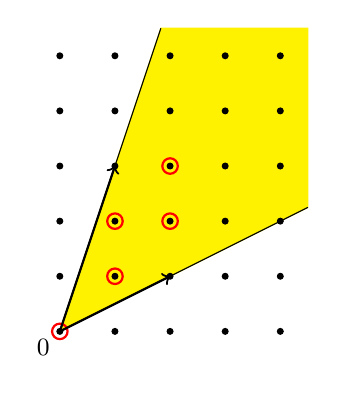
\begin{tikzpicture}[scale=0.7]
	\filldraw[yellow] (0,0) -- (1.833,5.5) -- (4.5,5.5) -- (4.5,2.25) -- cycle;
	\draw (0,0) -- (1.833,5.5);
	\draw (0,0) -- (4.5,2.25) node at (-0.3,-0.3){\small $0$};
	\foreach \x in {0,...,4}
	\foreach \y in {0,...,5}
	{
		\filldraw[fill=black] (\x,\y)  circle (1.5pt);
	}
	\draw[red,thick] (1,1) circle (4pt);
	\draw[red,thick] (2,3) circle (4pt);
	\draw[red,thick] (1,2) circle (4pt);
	\draw[red,thick] (2,2) circle (4pt);
	\draw[red,thick] (0,0) circle (4pt);
	\draw[->,thick] (0,0) -- (1,3);
	\draw[->,thick] (0,0) -- (2,1);
	\end{tikzpicture}
\end{center}
As an example, we can run \verb|2cone.in| with the option \verb|-M| on the command line. This yields the output
\begin{Verbatim}
...
4 Hilbert basis elements:                                      
 1 1                                                           
 1 2                  5 module generators over original monoid:
 1 3                   0 0                                     
 2 1                   1 1                                     
                       1 2                                     
2 extreme rays:        2 2                                     
 1 3                   2 3                                     
 2 1                                                           
\end{Verbatim} 

In the nonpointed case Normaliz can only compute the module generators of $N/N_0$ over $M/(M\cap N_0)$ where $N_0$ is the unit group of $N$. If $M_0\neq M_0$, this is not a system of generators of $M$ over $N$.

\subsubsection{An inhomogeneous example}

Let us have a look at a very simple input file (\verb|genmod_inhom2.in|):
\begin{Verbatim}
amb_space 2
cone 2
0 3
2 0
vertices 1
0 0 1
ModuleGeneratorsOverOriginalMonoid
\end{Verbatim}

The cone is the positive orthant that we have turned into a polyhedron by adding the vertex $(0,0)$. The original monoid is generated by $(2,0)$ and $(0,3)$. 

In addition to the original monoid $M$ and its integral closure $N$ we have a third object, namely the module $P$ of lattice points in the polyhedron.We compute
\begin{enumerate}
\item the system of generators of $P$ over $N$ (the \verb|module generators|) and
\item the system of generators of $P$ over $N$ (the \verb|module generators over original monoid|). 
\end{enumerate}
We do not compute the system of generators of $N$ over $M$ (that we get in the homogeneous case).

The output:
\begin{Verbatim}
1 module generators
2 Hilbert basis elements of recession monoid
1 vertices of polyhedron
2 extreme rays of recession cone
6 module generators over original monoid
3 support hyperplanes of polyhedron (homogenized)

embedding dimension = 3
affine dimension of the polyhedron = 2 (maximal)
rank of recession monoid = 2
internal index = 6

size of triangulation   = 1
resulting sum of |det|s = 6

dehomogenization:
0 0 1 


module rank = 1

***********************************************************************

1 module generators:
 0 0 1

2 Hilbert basis elements of recession monoid:
 0 1 0
 1 0 0

1 vertices of polyhedron:
 0 0 1

2 extreme rays of recession cone:
 0 1 0
 1 0 0

6 module generators over original monoid:
 0 0 1
 0 1 1
 0 2 1
 1 0 1
 1 1 1
 1 2 1

3 support hyperplanes of polyhedron (homogenized):
 0 0 1
 0 1 0
 1 0 0
\end{Verbatim}

\subsection{Lattice points in the fundamental parallelepiped}\label{LattPointsFPE}

Let $u_1,\dots,u_n$ be linearly independent vectors in $\ZZ^d\subset\RR^d$. They span a simplicial cone $C$. Moreover let $U$ be the subgroup of $(\RR^d,+)$ generated by $u_1,\dots,u_n$ and let $v\in\RR^d$. We are interested in the shifted cone $C'=v+C$. We assume that $C'$ contains a lattice point. This need not be true if $n<s$, but with our assumption we can also assume that $n=d$ after the restriction to the affine space spanned by $C'$. The \emph{fundamental} parallelepiped of $C$ (with respect to $U$) is
$$
F=\para(u_1,\dots,u_d)=\{q_qu_1+\dots+q_du_d: 0\le q_i<1  \}.
$$
Set $F'=v+F$. Then the translates $u+F'$, $u\in U$, tile $\RR^d$; so $F'$ is a fundamental domain for the action of $U$ on $\RR^d$ by translation, and we call it $F'$ the \emph{fundamental} parallelepiped of $C'$  (with respect to $U$). Every point in $\RR^d$ differs from exactly one point in $F'$ by an element of $U$. This holds in particular for the lattice points.

One of the main basic tasks if Normaliz is the computation of the lattice points in $F'$, especially in the case $v=0$ (but not only). Looking back at the examples in Section \ref{MinMod}, we see that we can in fact compute and export these lattice points via the computation goal \verb|ModuleGeneratorsOverOriginalMonoid|. 

Often however, an additional complication comes up: we  must shift $F'$ by an infinitesimally small vector in order to exclude certain facets of $C'$. This would be difficult in Normaliz without the input type \verb|open_facets| (see Section \ref{open_facets}). Recall that this is a $0$-$1$-vector whose entries $1$ indicate which facets must be avoided: if its $i$-th entry is $1$, then the facet opposite to $v+u_i$ must be made `open''.

The input file \verb|no_open_facets.in| is
\begin{Verbatim}
amb_space 2
cone 2
1 1
-3 3
vertices 1
1/2 1/2 1
ModuleGeneratorsOverOriginalMonoid
\end{Verbatim}

Then \verb|no_open_facets.out| contains
\begin{Verbatim}
6 module generators over original monoid:
-2 3 1
-1 2 1
-1 3 1
 0 1 1
 0 2 1
 1 1 1
\end{Verbatim}
These are $6$ encircled points in the left figure.

\begin{center}
	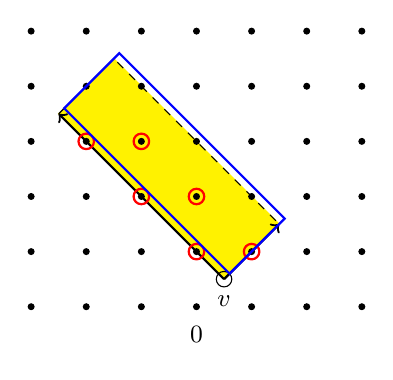
\begin{tikzpicture}[scale=0.7]
	\filldraw[yellow] (0.5,0.5) -- (1.5,1.5) -- (-1.5,4.5) -- (-2.5,3.5) -- cycle;
	\foreach \x in {-3,...,3}
	\foreach \y in {0,...,5}
	{
		\filldraw[fill=black] (\x,\y)  circle (1.5pt);
	}
	\draw[->,thick] (0.5,0.5) -- (-2.5,3.5);
	\draw[->,thick] (0.5,0.5) -- (1.5,1.5);
	\draw[dashed] (-2.5,3.5) -- (-1.5,4.5) -- (1.5,1.5);
	\draw node at (0,-0.5){\small $0$};
	\draw node at (0.5,0.1){\small $v$};
	\draw[red,thick] (1,1) circle (4pt);
	\draw[red,thick] (0,1) circle (4pt);
	\draw[red,thick] (-1,2) circle (4pt);
	\draw[red,thick] (0,2) circle (4pt);
	\draw[red,thick] (-2,3) circle (4pt);
	\draw[red,thick] (-1,3) circle (4pt);
	\draw (0.5,0.5) circle (4pt);
	\draw[blue, thick] (0.6,0.6) -- (1.6,1.6) -- (-1.4,4.6) -- (-2.4,3.6) -- cycle;
	\end{tikzpicture}
\qquad\qquad\qquad
	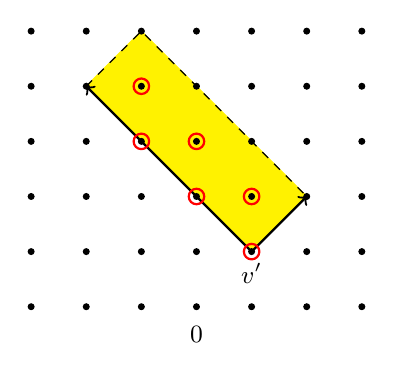
\begin{tikzpicture}[scale=0.7]
	\filldraw[yellow] (1,1) -- (2,2) -- (-1,5) -- (-2,4) -- cycle;
	\foreach \x in {-3,...,3}
	\foreach \y in {0,...,5}
	{
		\filldraw[fill=black] (\x,\y)  circle (1.5pt);
	}
	\draw[->,thick] (1,1) -- (-2,4);
	\draw[->,thick] (1,1) -- (2,2);
	\draw[dashed] (-2,4) -- (-1,5) -- (2,2);
	\draw node at (0,-0.5){\small $0$};
	\draw node at (1,0.6){\small $v'$};
	\draw[red,thick] (1,1) circle (4pt);
	\draw[red,thick] (1,2) circle (4pt);
	\draw[red,thick] (0,3) circle (4pt);
	\draw[red,thick] (0,2) circle (4pt);
	\draw[red,thick] (-1,4) circle (4pt);
	\draw[red,thick] (-1,3) circle (4pt);
	\end{tikzpicture}
\end{center}
Now we add 
\begin{Verbatim}
open_facets 
1 0
\end{Verbatim}
to the input (to get \verb|open_facets.in|). We have tried to indicate the infinitesimal shift by the blue rectangle in the left figure. The computation yields
\begin{Verbatim}
6 module generators over original monoid:
-1 3 1
-1 4 1
0 2 1
0 3 1
1 1 1
1 2 1
\end{Verbatim}
which are the encircled lattice points in the right figure. It is explained in Section \ref{open_facets} how the new vector $v'$ is computed.

Note that the lattice points are listed with the homogenizing coordinate $1$. In fact, both \verb|vertices| and \verb|open_facets| make the computation inhomogeneous. If both are missing, then the lattice points are listed without the homogenizing coordinate. If you want a uniform format for the output, you can use the zero vector for \verb|open_facets| or the origin as the vertex. Both options change the result only to the extent that the homogenizing coordinate is added.

\subsection{Precomputed data}

The input of precomputed data can be useful if their computation takes long and they can be used again in subsequent computations. Normaliz takes their correctness for granted since there is no way of checking it without recomputation.

\subsubsection{Support hyperplanes}\label{supphyp_ex}

They are formally introduced in Section \ref{HomConstrCone}.
The file \verb|2cone_supp.in| is just a toy example:
\begin{Verbatim}
amb_space 2
cone 2
2 1
1 3
support_hyperplanes 2
-1  2
 3 -1
\end{Verbatim}

Note: (i) the input type \verb|support_hyperplanes| is only allowed together with homogeneous input.

(ii) They are not used in the definition of the cone. However, once the cone is defined (by generators or constraints), they override any other inequalities that are implicitly or explicitly given in the input. \verb|excluded_faces| are an exception; they remain excluded.

\subsubsection{Extreme rays} \label{extrays_ex}

They are formally introduced in Section \ref{cone_synt}. Again we give only a toy example in \verb|2cone_ext.in|:
\begin{Verbatim}
amb_space 2
inequalities 2
-1  2
3 -1
extreme_rays 2
2 1
1 3
\end{Verbatim}

Note: (i) the input type \verb|extreme_rays| is only allowed together with homogeneous input.

(ii) They are not used in the definition of the cone. However, once the cone is defined (by generators or constraints), they override any other cone generators. They are not considered to be generators of the original monoid.

\subsubsection{Hilbert basis of the recession cone}

In applications one may want to compute several polyheda with the same recession cone. In these cases it is useful to add the Hilbert basis of the recession cone to the input. An example is \verb|small_inhom_hbrc.in|:
\begin{Verbatim}
amb_space 6
cone 190
6 0 7 0 10 1
...
vertices 4
0 0 0 0 0 0 1
1 2 3 4 5 6 2
-1 3 9 8 7 1 3
0 2 4 5 8 10 7
hilbert_basis_rec_cone 34591
0  0  0  1  6 1 0
0  0  0  1  7 1 0
...
\end{Verbatim}
As in the other cases with precomputed data, Normaliz must believe you and the precomputed Hilbert basis of the recession cone does not define the latter.

It requires inhomogeneous input. Note that it can only be used in the primal algorithm. In the dual algorithm it is useless and therefore ignored.  


\section{Algebraic polyhedra} \label{Algebraic}

Normaliz can use coefficients from real algebraic extensions of $\QQ$. It is clear that the computations are then restricted to those that do not depend on finite generation of monoids.  Whether algebraic coordinates are needed, is decided when Normaliz reads the input file and checks whether it defines an algebraic extension of $\QQ$ embedded into $\RR$.

\subsection{An example}\label{alg_ex}

The icosahedron, one of the platonic solids, needs $\sqrt 5$ for its coordinates. Via its vertices it can be defined as follows (\verb|icosahedron-v.in|)
\begin{verbatim}
amb_space 3
number_field min_poly (a^2 - 5) embedding [2 +/- 1]
vertices 12
0 2 (a + 1) 4
0 -2 (a + 1) 4
2 (a + 1) 0 4
...
(-a - 1) 0 -2 4
Volume
ModuleGenerators
FVector
\end{verbatim}

The second line specifies the extension $\QQ[\sqrt 5]$ of $\QQ$ over which we want to define the icosahedron. In addition to the minimal polynomial (\verb|min_poly| or \verb|minpoly|)we have to give an interval from which the zero of the polynomial is to be picked. The square brackets are mandatory. There must be a \emph{single} zero in that interval. The name of the root is fixed to be \verb|a|. The number field specification must follow \verb|amb_space|. Otherweise Normaliz believes that you want to work over $\ZZ$. 

Note that the entries of the input file that contain \verb|a| must be enclosed in round brackets. You can enter any $\QQ$-linear combination of powers of \verb|a|. We allow \verb|*| between the coefficient and the power of \verb|a|, but it need not appear. The character \verb|^| indicates the exponent. It is mandatory. So
\begin{Verbatim}
(a^3-2*a^2  +   4a-1/2)
(a+a-2a-10 + 10*a^0)
\end{Verbatim}
are legal matrix entries.

The result of the computation by \verb|normaliz -c ../example/icosahedron-v| starts
\begin{Verbatim}
Real embedded number field:
min_poly (a^2 - 5) embedding [2.2360679774997896964091736687312762354 +/- 5.73e-38]
\end{Verbatim}
It indicates that the precision to which the root had to be computed in order to decide all the inequalities that have come up in the computation. Then we go on as usual:

\begin{Verbatim}
12 vertices of polyhedron
0 extreme rays of recession cone
20 support hyperplanes of polyhedron (homogenized)

f-vector:
1 12 30 20 1 

embedding dimension = 4
affine dimension of the polyhedron = 3 (maximal)
rank of recession cone = 0

size of triangulation   = 18
resulting sum of |det|s = (5/2*a+15/2 ~ 13.090)

dehomogenization:
0 0 0 1 

volume (lattice normalized) = (5/2*a+15/2 ~ 13.090)
volume (Euclidean) = 2.18167
\end{Verbatim}
From the vertices below you can compute the radius of the sphere in which the icosahedron is inscribed and check that it is $<1$. So no surprise:
\begin{Verbatim}
1 lattice points in polytope:
0 0 0 1

12 vertices of polyhedron:
(-1/4*a-1/4 ~ -0.80902)                       0        (-1/2 ~ -0.5000) 1
 ...
  (1/4*a+1/4 ~ 0.80902)                       0        (-1/2 ~ -0.5000) 1
  (1/4*a+1/4 ~ 0.80902)                       0          (1/2 ~ 0.5000) 1

0 extreme rays of recession cone:

20 support hyperplanes of polyhedron (homogenized):
(-a+1 ~ -1.2361) (-2*a+4 ~ -0.47214)                   0 1
...
  (a-1 ~ 1.2361) (-2*a+4 ~ -0.47214)                   0 1
  (a-1 ~ 1.2361)   (2*a-4 ~ 0.47214)                   0 1
\end{Verbatim}
Now every nonintegral number appears in round brackets together with its approximation as a decimal fraction.

The data of the integer hull cone are printed into a separate file as usual.

The matrices in the (optional) output file(s) can be used as input; see \verb|perm7_d2_dual.in|. The input routine skips all characters from \verb|~| when it reads a number. 

\subsection{Input}}\label{alg_inp}

The following input types are NOT allowed for algebraic polytopes:
\begin{center}
\texttt{
\begin{tabular}{llll}
lattice &strict\_inequalities&strict\_signs&open\_facets\\
cone\_and\_lattice& inhom\_congruences& lattice\_ideal&offset\\
congruences& hilbert\_basis\_rec\_cone& excluded\_faces
\end{tabular}
}
\end{center}
The only other restriction is that decimal fractions and floating point numbers are not allowed in the input file. The input format for field coefficients is explained in the example above.

It may seem contradictory, but  \verb|saturation| is allowed. It must be interpreted as a generating set for a subspace that is intersected with all the objects defined by other input items.

With coordinates in number fields, Normaliz does not look for an implicit grading, but it can use an explicit grading for lattice point or volume computations in the homogeneous case. \ttt{NoGradingDenom} is set automatically.  For inhomogeneous input a grading makes no sense in the number field case and is therefore forbidden.

\subsection{Computations}\label{alg_comp}

The only (main) computation goals and algorithmic variants allowed are:
\begin{center}
\texttt{
\begin{tabular}{llll}
SupportHyperplanes & Sublattice & LatticePoints&Deg1Elements \\
NumberLatticePoints& IntegerHul&VerticesFloat&SuppHypsFloat\\
Triangulation& TriangulationDetSum &TriangulationSize &  ConeDecomposition\\
BottomDecomposition&KeepOrder & NoBottomDec &ProjectCone\\
GradingIsPositive&DefaultMode& IsPointed&FaceLattice\\
FVector
\end{tabular}	}
\end{center}

It may seem paradoxical that \verb|Sublattice| appears here. As in the true lattice case, the \verb|Sublattice| \verb|Representation| is  the coordinate transformation used by Normaliz. Over a field $F$ there is no need for the annihilator $c$, and one simply has a pair of linear maps $F^r\to F^d \to F^r$ whose composition is the identity of $F^r$. Of course, congruences and external index make no sense anymore.

\verb|Deg1Elements|, \verb|LatticePoints| and \verb|IntegerHull| are restricted to (bounded) polytopes since polyhedra in general lack the necessary finiteness properties. The lattice of reference is the full integral lattice.

\verb|Volume| is restricted to full-dimensional polytopes. In the homogeneous case the grading must have integer coprime coefficients.

The only algorithmic variants that appear concern the bottom decomposition. Implicit or explicit \verb|DefaultMode| is interpreted as \verb|SupportHyperplanes|.

Volumes are computed by triangulation and lattice points by project-and-lift.

For the control of computations and communication with interfaces the following are allowed:
\begin{center}
\texttt{
\begin{tabular}{llll}
Generators& ExtremeRays & VerticesOfPolyhedron & MaximalSubspace \\
RecessionRank & AffineDim&  Rank&    EmbeddingDim\\
IsInhomogeneous &RenfVolume  &EuclideanVolume	&ModuleGenerators\\
Dehomogenization&NoGradingDenom&Equations\\
\end{tabular}	}
\end{center}

\subsection{Restrictions in MS Windows}

Algebraic polytopes are not computable in MS Windows. The ways out are (1) the Docker image and (2) the statically compiled Linux binary run in the Linux subsystem of MS Windows.


\section{Optional output files}\label{optionaloutput}

Note that the options \verb|-T, Triangulation| and \verb|-y, StanleyDec|  also write files in addition to \verb|<project>.out|, as well as \verb|FaceLattice|. Also symmetrization and \verb|IntegerHull| produce extra output files for the derived cones. But these are \emph{not} optional.

When one of the options \ttt{Files,-f} or \ttt{AllFiles, -a} is activated, Normaliz
writes additional optional output files whose names are of type
\ttt{<project>.<type>}. Moreover one can select the optional output files individually on the command line. Most of these files contain matrices in a simple format:
\begin{Verbatim}
<m>
<n>
<x_1>
...
<x_m>
\end{Verbatim}
where each row has \verb|<n>| entries. Exceptions are the files with suffixes \verb|cst|, \verb|inv|, \verb|esp|.

Note that the files are only written if they would contain at least one row.

As pointed out in Section \ref{outcontrol}, the optional output files for the integer hull are the same as for the original computation, as far as their content has been computed.

\subsection{The homogeneous case}

The option \ttt{-f} makes Normaliz write the following files:

\begin{itemize}
\itemtt[gen] contains the Hilbert basis. If you want to use this file as an input file and reproduce the computation results, then you must make it a matrix of type \verb|cone_and_lattice| (and add the dehomogenization in the inhomogeneous case).

\itemtt[cst] contains the constraints defining the cone
and the lattice in the same format as they would appear
in the input: matrices of types \emph{constraints} following each
other. Each matrix is concluded by the type of the constraints.
Empty matrices are indicated by $0$ as the
number of rows. Therefore there will always be at least
$3$ matrices.

If a grading is defined, it will be appended. Therefore
this file (with suffix \ttt{in}) as input for
Normaliz will reproduce the Hilbert basis and all the
other data computed, at least in principle.

In the case of number field coordinates this file must be transformed from Normaliz~2 input format to Normaliz 3 format by hand before it can be used for input.

\itemtt[inv]  contains all the information from the
file \ttt{out} that is not contained in any of the
other files.
\end{itemize}

If \ttt{-a} is activated, then the following files are written
\emph{additionally:}

\begin{itemize}

\itemtt[ext] contains the extreme rays of the cone.

\itemtt[ht1] contains the degree $1$ elements of the
Hilbert basis if a grading is defined.

\itemtt[egn,esp] These contain the Hilbert basis and
support hyperplanes in the coordinates with respect to
a basis of $\EE$. \ttt{esp} contains the grading and the dehomogenization in the
coordinates of $\EE$. Note that no
equations for $\CC\cap\EE$ or congruences for $\EE$ are
necessary.

\itemtt[lat] contains the basis of the lattice $\EE$.

\itemtt[mod] contains the module generators of the integral closure modulo the original monoid.

\itemtt[msp] contains the basis of the maximal subspace.
\end{itemize}

In order to select one or more of these files individually, add an option of type \verb|--<suffix>| to the command line where \verb|<suffix>| can take the values
\begin{Verbatim}
gen, cst, inv, ext, ht1, egn, esp, lat, mod, msp, typ
\end{Verbatim}

The type \verb|typ| is not contained in \verb|Files| or \verb|AllFiles| since it can be extremely large. It is of the matrix format described above. It is the product of the matrices
corresponding to \ttt{egn} and the transpose of \ttt{esp}. In other
words, the linear forms representing the support
hyperplanes of the cone $C$ are evaluated on the
Hilbert basis. The resulting matrix, with the
generators corresponding to the rows and the support
hyperplanes corresponding to the columns, is written to
this file.

The suffix \ttt{typ} is motivated by the fact that the
matrix in this file depends only on the isomorphism
type of monoid generated by the Hilbert basis (up to
row and column permutations). In the language of
\cite{BG} it contains the \emph{standard embedding}. 

Note: the explicit choice of an optional output file does \emph{not} imply a computation goal. Output files that would contain unknown data are simply not written without a warning or error message.

\subsection{Modifications in the inhomogeneous case}

The optional output files  are a subset of those that can be produced in the homogeneous
case. The main difference is that the generators of the solution module and the
Hilbert basis of the recession monoid appear together in the file \verb|gen|.
They can be distinguished by evaluating the dehomogenization on them (simply the last component with inhomogeneous input), and the
same applies to the  vertices of the polyhedron and extreme rays of the
recession cone. The file \verb|cst| contains the constraints defining the
polyhedron and the recession module in conjunction with the dehomogenization, which is also contained in the \verb|cst| file, following the constraints.

With \verb|-a| the files \verb|egn| and \verb|esp| are produced. These files contain \verb|gen| and the support hyperplanes of the homogenized cone in the coordinates of $\EE$, as well as the dehomogenization.

\section{Performance}\label{Perf}

\subsection{Parallelization}\label{PerfPar}

The executables of Normaliz have been compiled for parallelization
on shared memory systems with OpenMP. Parallelization reduces the
``real'' time of the computations considerably, even on relatively
small systems. However, one should not underestimate the
administrational overhead involved.
\begin{itemize}
\item It is not a good idea to use parallelization for very small problems.
\item On multi-user systems with many processors it may be wise to limit
the number of threads for Normaliz somewhat below the maximum
number of cores.
\end{itemize}
By default, Normaliz limits the number of threads to 8. One can override this limit by the Normaliz
option \ttt{-x} (see Section \ref{exec}).

Another way to set an upper limit to the number of threads is via the environment variable \verb|OMP_NUM_THREADS|:
\begin{center}
	\verb+export OMP_NUM_THREADS=<T>+\qquad (Linux/Mac)
\end{center}
or
\begin{center}
	\verb+set OMP_NUM_THREADS=<T>+\qquad (Windows)
\end{center}
where \ttt{<T>} stands for the maximum number of threads
accessible to Normaliz. For example, we often use
\begin{center}
	\verb+export OMP_NUM_THREADS=20+
\end{center}
on a multi-user system system with $24$ cores.

Limiting the number of threads to $1$ forces a strictly serial
execution of Normaliz.

The paper \cite{BIS} contains extensive data on the effect of parallelization. On the whole Normaliz scales very well.
However, the dual algorithm often performs best with mild parallelization, say with $4$ or $6$ threads.

\subsection{Running large computations}\label{Large}

Normaliz can cope with very large examples, but  it
is usually difficult to decide a priori whether an example is
very large, but nevertheless doable, or simply impossible.
Therefore some exploration makes sense. The following applies to the primal algorithm.

See \cite{BIS} for some very large computations. The following
hints reflect the authors' experience with them.

(1) Run Normaliz with the option \ttt{-cs} and pay attention
to the terminal output. The number of extreme rays, but also
the numbers of support hyperplanes of the intermediate cones
are useful data.

(2) In many cases the most critical size parameter for the primal algorithm is the
number of simplicial cones in the triangulation. It makes sense
to determine it as the next step. Even with the fastest
potential evaluation (option \ttt{-v} or \verb|TriangulationDetSum|), finding the
triangulation takes less time, say by a factor between $3$ and
$10$. Thus it makes sense to run the example with \ttt{-t} in
order to explore the size.

As you can see from \cite{BIS}, Normaliz has successfully
evaluated triangulations of size $\approx 5\cdot 10^{11}$ in
dimension $24$.

(3) Another critical parameter are the determinants of the
generator matrices of the simplicial cones. To get some feeling
for their sizes, one can restrict the input to a subset (of the
extreme rays computed in (1)) and use the option \ttt{-v} or the computation goal \verb|TriangulationDetSum| if there is no grading.

The output file contains the number of simplicial cones as well
as the sum of the absolute values of the determinants. The
latter is the number of vectors to be processed by Normaliz
in triangulation based calculations.

The number includes the zero vector for every simplicial cone
in the triangulation. The zero vector does not enter the
Hilbert basis calculation, but cannot be neglected for the
Hilbert series.

Normaliz has mastered calculations with $> 10^{15}$ vectors.

(4) If the triangulation is small, we can add the option
\ttt{-T} in order to actually see the triangulation in a file.
Then the individual determinants become visible.

(5) If a cone is defined by inequalities and/or equations
consider the dual mode for Hilbert basis calculation, even if
you also want the Hilbert series.

(6) The size of the triangulation and the size of the
determinants are \emph{not} dangerous for memory by themselves
(unless \ttt{-T} or \ttt{-y} are set). Critical magnitudes can
be the number of support hyperplanes, Hilbert basis candidates,
or degree $1$ elements.


%%%%%%%%%%%%%%%%%%%%%%%%%%%%%  DISTRIBUTION  %%%%%%%%%%%%%%%%%%%%%%%%%%%%%
\section{Distribution and installation}\label{Distr}

\subsection{Docker image}
The easiest and absolutely hassle free access to Normaliz is via its Docker image. To run it, you must first install Docker on your system. This is easy on up-to-date versions of the three major platforms. After installation you can issue the command 
\begin{Verbatim}
docker run -ti normaliz/normaliz
\end{Verbatim}
This will download the Docker image if it is not yet present and open a Docker container. As a result you will get a Linux terminal. Normaliz is installed in the standard location \verb|/usr/local|. Moreover, the source is contained in the subdirectory \verb|Normaliz| of the home directory. (Your username is \verb|norm.|) In the Docker container \verb|Normaliz| is the Normaliz directory (independently of the version number).

Try
\begin{Verbatim}
normaliz -c Normaliz/exampe/small
\end{Verbatim}
as a first test.

Of course, you want to make your data available to Normaliz in the container. The Docker documentation tells you how to do it.

The command above downloads the image labeled ``latest''. It is produced from the branch ``release'' on GitHub, which always contains the latest official release. There is a second image, produced from the branch ``master''. It is updated with every commit to this branch. You can get it by appending \verb|:master| to the command above.

The Docker image contains a full installation including PyNormaliz and PyQNormaliz.

\subsection{Basic package}
In order to install Normaliz you should first download the
basic package. Follow the instructions in
\begin{center}
\url{http://normaliz.uos.de/download/}.
\end{center}
They guide you to our GitHub repository
\begin{center}
	\url{https://github.com/Normaliz/Normaliz/releases}.
\end{center}

The full version \ttt{\NmzDir-full.zip} of the basic package contains the documentation, examples, source
code, jNormaliz, and the packages for PyNormaliz, Singular
and Macaulay2. 


The minimal version \ttt{\NmzDir.zip} (also available as \ttt{.tar.gz}) contains the source files, examples, documentation and PyNormaliz.

Then unzip the downloaded file in a directory of your choice. (Any other
downloaded zip file for Normaliz should be unzipped in this
directory, too.)

This process will create a directory \ttt{\NmzDir} (called
Normaliz directory) and several subdirectories in
it. The names of the subdirectories created are
self-explanatory. Nevertheless we give an overview:
\begin{itemize}
\item In the Normaliz directory you should
find \ttt{jNormaliz.jar}, several files, for example installation scripts mentioned below,  and
subdirectories.

\item The subdirectory \ttt{source} contains the source files.

\item The subdirectory \ttt{doc} contains the file you are reading 
and further documentation.

\item In the subdirectory \ttt{example} are the input
files for some examples. It contains all named
input files of examples of this manual.

\item Automated tests which run Normaliz on different inputs
and options are contained in the subdirectory \ttt{test}.

\item The subdirectory \ttt{Singular} contains the
\textsc{Singular} library \ttt{normaliz.lib} and a PDF file with
documentation.

\item The subdirectory \ttt{Macaulay2} contains the
\textsc{Macaulay2} package \ttt{Normaliz.m2}.

\item The subdirectory \ttt{PyNormaliz} contains the source
\textsc{Python} interface.

\item The subdirectory \ttt{lib} contains libraries for
jNormaliz.

\item The subdirectory \verb|install_scripts_opt| contains scripts for the installation of optional packages.
jNormaliz.
\end{itemize}

If you build Normaliz yourself, ubdirectories \verb|nmz_opt_lib| and \verb|local| will be created (with rthe fefault settings).

\subsection{Executables}

We provide executables for Windows, Linux and Mac. Download the archive file
corresponding to your system \ttt{\NmzDir<systemname>.zip}
and unzip it. This process will store the Normaliz executable in the Normaliz directory. In case you want to run Normaliz from the
command line or use it from other systems, you may have to copy
the executables to a directory in the search path for
executables or update your search path.

The MS Windows executable is compiled without any optional package; in particular there are no algebraic polytopes. However, the Linux 64 binary runs in the Linux subsystem of Windows 10. It is extremely easy to install the Linux subsystem.

Note:
\begin{enumerate}
\item The linux binariy \verb|normaliz| is a truly static executable. 

\item The Mac OS binary cannot be statically linked in the absolute sense, but it depends only on Mac OS system libraries and \verb|libomp.dylib| (contained in the zip file) which makes parallelization possible. This dynamic library must be kept in the same directoory as the binary.

\item For MS Windows we provide \verb|libiomp5md.dll| for parallelization. Keep it in the same directory as \verb|normaliz.exe|.
\end{enumerate}

\subsection{Cloning the GitHub repository}

Another way to download the Normaliz source is cloning the repository from GitHub by
\begin{Verbatim}
git clone https://github.com/Normaliz/Normaliz.git
\end{Verbatim}
The Normaliz directory is then called \verb|Normaliz|. You may need
\begin{Verbatim}
sudo apt-get install autoconf libtool
\end{Verbatim}
if you want to build Normaliz by autotools. To this end change to the Normaliz directory and run
\begin{Verbatim}
./bootstrap.sh
\end{Verbatim}
After this step you can follow the instruction in the next section.

Note that he GitHub repository Normaliz/Normaliz does not contain Py(Q)Normaliz. You can clone them from the repositories Normaliz/PyNormaliz and Normaliz/PyQNormaliz.

%%%%%%%%%%%%%%%%%%%%%%%%%%%%%  COMPILATION  %%%%%%%%%%%%%%%%%%%%%%%%%%%%%
\section{Building Normaliz yourself}\label{Compile}

We recommend building Normaliz through the install scripts described below. They use the \verb|autotools| scripts have been written by Matthias K\"oppe. The Normaliz team thanks him cordially for his generous help.

\verb|cmake| is no longer supported. 

\subsection{Prerequisites}

We require some C++11 features (e.g. \verb|std::exception_ptr|), supported by:
\begin{itemize}
	\item GNU g++ 4.4,
	\item clang++ 2.9,
	\item Intel icpc 12.0
\end{itemize}
See \url{https://github.com/Normaliz/Normaliz/issues/26} for a more detailed discussion.

The mentioned compilers are also able to handle OpenMP 3.0, with the exception of clang++, there the first OpenMP support was introduced in 3.7.

For compiling Normaliz the following libraries are needed:
\begin{itemize}
	\item GMP including the C++ wrapper (libgmpxx and libgmp)
	\item Boost (headers only)
\end{itemize}

We will only discuss how to build Normaliz with the install scrips in the distribution. See the file \verb|INSTALL| for additional information. 

Any optional package that you want to use, must be installed before the compilation of Normaliz, independently of the method used for building Normaliz. The installation scripts mentioned below make and use directories within the Normaliz directory.

\subsubsection{Linux}
The standard compiler choice on Linux is \verb|g++|. We do no not recommend \verb|clang++| since its support for OpenMP is not as comprehensive as that of \verb|g++|.

On Ubunto we suggest
\begin{Verbatim}
sudo apt-get install tar g++ libgmp-dev libboost-dev wget make
\end{Verbatim}
for the basic installation of the required libraries (plus compiler).

\subsubsection{Mac OS X}\label{mac}

Currently Apple does not supply a compiler which supports OpenMP.
The install scripts discussed below \emph{require LLVM 3.9 or newer from Homebrew.} See
\url{http://brew.sh/} from where you can also download GMP and Boost:

\begin{Verbatim}
brew install gmp boost llvm wget
\end{Verbatim}

You also need to download and install the Xcode Command Line Tools from the AppStore:
\begin{Verbatim}
xcode-select --install
\end{Verbatim} 

\subsection{Normaliz at a stroke}\label{stroke}

Navigate to the Normaliz directory. The command
\begin{Verbatim}
./install_normaliz_with_eantic.sh
\end{Verbatim}
installs the all packages that are needed for the computation of rational and algebraic polytopes (including CoCoALib and Flint) and does the full compilation.

If you don't want algebraic polyhedra, call
\begin{Verbatim}
./install_normaliz_with_opt.sh
\end{Verbatim}
It downloads CoCoALib and Flint and compiles Normaliz.

The sources of the optional packages are downloaded to the subdirectory \verb|nmz_opt_lib| of the Normaliz directory. They are installed in the subdirectory \verb|local| (imitating \verb|/usr/local|) where they exist in static and dynamic versions (except CoCoALib that can only be built statically).

If you don't want the optional packages or if you have them properly installed,
\begin{Verbatim}
./install_normaliz.sh
\end{Verbatim}
compiles Normaliz, using the optional packages that it can find. 

The library \verb|libnormaliz| is compiled statically and shared. It is installed in \verb|local| as well. 

The binary \verb|normaliz| is stored in \verb|local/bin|, but it is also copied to the Normaliz directory. It is not linked statically, but depends only on shared objects provided by the operating system. 

Remarks:
\begin{arab}
\item By
\begin{Verbatim}
export NMZ_SHARED=yes  
./install_normaliz_...
\end{Verbatim}
one can build Normaliz completely with shared libraries.
\item It is possible to compile a statically linked Linux version of  \verb|normaliz|  through the \verb|Makefile.classic| in the directoriy \verb|source| after the installation of the optional libaries.

\item If you want a global installation (and have the rights to do it), you can ask for
\begin{Verbatim}
sudo cp -r local /usr
\end{Verbatim}
at the end.

\item Another way to a global installation (or to an installation in a place of your choice) is to use
\begin{Verbatim}
export NMZ_PREFIX=<your choice>  
./install_normaliz_...
\end{Verbatim}

For the typical choice \verb|/usr/local| you need superuser rights (as in (4)). Note that \verb|NMZ_PREFIX| must be an absolute path name.

\item The install scripts can be further customized. Have a look at them or at \verb|INSTALL|.

\item Precise information on the versions of the optional packages that should be used with Normaliz \version{} is contained in \verb|INSTALL| as well.
\end{arab}

\subsection{Packages for rational polyhedra}

\subsubsection{CoCoALib}

Normaliz can be built without CoCoALib, which is however necessary for the computation of integrals and weighted Ehrhart series and, hence,  for symmetrization. If you don't want to use the scripts in Section \ref{stroke}, but nevertheless want to compile Normaliz with CoCoALib, install  CoCoALib first by navigating to the Normaliz directory and typing the command
\begin{Verbatim}
./install_scripts_opt/install_nmz_cocoa.sh
\end{Verbatim}
CoCoALib is downloaded and compiled as described above.

\subsubsection{Flint}

Flint does not extend the functionality of Normaliz, and is therefore truly optional.
However, the ultrafast polynomial arithmetic of Flint is very useful if quasipolynomials with large periods come up in the computation of Hilbert series or weighted Ehrhart series. If you don't want to use the scripts in Section \ref{stroke}, but nevertheless want to compile Normaliz with Flint,  install Flint (and MPFR) navigating to the Normaliz directory and typing the command
\begin{Verbatim}
./install_scripts_opt/install_nmz_flint.sh
\end{Verbatim}

\subsubsection{SCIP}

As discussed in the manual, Normaliz can use SCIP, but Normaliz' own method seems to be superior. See the file \verb|INSTALL|  for instructions on the use of SCIP.
 
\subsection{Packages for algebraic polyhedra}

The basic classes for algebbraic polyhedra are defined in the package
\begin{itemize}
	\item[]  e-antic by V. Delecroix and M. K\"oppe (\url{https://github.com/videlec/e-antic}).
\end{itemize}
In its turn it is based on
\begin{arab}
	\item Flint maintained by B. Hart (\url{http://www.flintlib.org/}),
	\item antic by B. Hart and F. Johansson, (\url{https://github.com/wbhart/antic}),
	\item arb by F. Johansson (\url{http://arblib.org/}).
\end{arab}

For Normaliz it is useless to install any of them separately. Again, if you don't want to use the ready-made install scripts, you can install e-antic and its prerequisites by
\begin{Verbatim}
./install_scripts_opt/install_eantic_with_prerequisites.sh
\end{Verbatim}

\subsection{MS Windows}

One can compile Windows executables with the Cygwin port of GCC. Unfortunately it is not compatible to OpenMP.

Using Visual Studio is a bit tricky. Microsoft's C++ compiler does not support OpenMP 3.0. Creating a Normaliz Visual Studio project via cmake is currently not fully supported. The executables that are offered in the Normaliz distribution have been compiled with Intel icpc and a manually created project. Please contact us if you want to build Normaliz on Windows.

MS Windows does not support any of the optional libraries of Normaliz. There are two ways out: (1) the Docker image or (2) the statically linked Linux binary. It runs in the Linux subsystem of Windows 10. ()We have not yet tried to build Normaliz in it.)

\section{Copyright and how to cite}

Normaliz 3.1 is free software licensed under the GNU General
Public License, version 3. You can redistribute it and/or
modify it under the terms of the GNU General Public License as
published by the Free Software Foundation, either version 3 of
the License, or (at your option) any later version.

It is distributed in the hope that it will be useful, but
WITHOUT ANY WARRANTY; without even the implied warranty of
MERCHANTABILITY or FITNESS FOR A PARTICULAR PURPOSE. See the
GNU General Public License for more details.

You should have received a copy of the GNU General Public
License along with the program. If not, see
\url{http://www.gnu.org/licenses/}.

Please refer to Normaliz in any publication for which it has
been used:
\begin{center}
	W. Bruns, B. Ichim, T. R\"omer, R. Sieg and C. S\"oger: Normaliz. Algorithms for
	rational cones and affine monoids. Available at
	\url{http://normaliz.uos.de}
\end{center}
The corresponding \verb|\bibitem|:
\begin{Verbatim}
\bibitem{Normaliz} W. Bruns, B. Ichim, T. R\"omer, R. Sieg and C. S\"oger:
Normaliz. Algorithms for rational cones and affine monoids.
Available at \url{http://normaliz.uos.de}.
\end{Verbatim}

A BibTeX entry:
\begin{Verbatim}
@Misc{Normaliz,
author = {W. Bruns and B. Ichim and T. R\"omer and R. Sieg and C. S\"oger},
title = Normaliz. Algorithms for rational cones and affine monoids,
howpublished ={Available at \url{http://normaliz.uos.de}}
\end{Verbatim}

It is now customary to evaluate mathematicians by such data as
numbers of publications, citations and impact factors. The data
bases on which such dubious evaluations are based do not list
mathematical software. Therefore we ask you to cite the article
\cite{BIS} in addition. This is very helpful for the younger
members of the team.

\newpage

\appendix

\section{Mathematical background and terminology}

For a coherent and thorough treatment of the mathematical background we refer the reader to \cite{BG}.

\subsection{Polyhedra, polytopes and cones}

An \emph{affine halfspace} of $\RR^d$ is a subset given as
$$
H_\lambda^+=\{x: \lambda(x)\ge 0\},
$$
where $\lambda$ is an affine form, i.e., a non-constant map $\lambda:\RR^d\to\RR$, $\lambda(x)=\alpha_1x_1+\dots+\alpha_dx_d+\beta$ with $\alpha_1,\dots,\alpha_d,\beta\in\RR$. If $\beta=0$ and $\lambda$ is therefore linear, then the halfspace is called \emph{linear}. The halfspace is \emph{rational} if $\lambda$ is \emph{rational},  i.e., has rational coordinates. If $\lambda$ is rational, we can assume that it is even \emph{integral}, i.e., has integral coordinates, and, moreover, that these are coprime. Then $\lambda$ is uniquely determined by $H_\lambda^+$. Such integral  forms are called \emph{primitive}, and the same terminology applies to vectors.

\begin{definition}
	A (rational) \emph{polyhedron} $P$ is the intersection of finitely many (rational) halfspaces. If it is bounded, then it is called a \emph{polytope}. If all the halfspaces are linear, then $P$ is a \emph{cone}.
	
	The \emph{dimension} of $P$ is the dimension of the smallest affine subspace $\aff(P)$ containing $P$.
\end{definition}


A support hyperplane of $P$ is an affine hyperplane $H$ that intersects $P$, but only in such a way that $H$ is contained in one of the two halfspaces determined by $H$. The intersection $H\cap P$ is called a \emph{face} of $P$. It is a polyhedron (polytope, cone) itself. Faces of dimension $0$ are called \emph{vertices}, those of dimension $1$ are called \emph{edges} (in the case of cones \emph{extreme rays}), and those of dimension $\dim(P)-1$ are \emph{facets}.

When we speak of \emph{the} support hyperplanes of $P$, then we mean those intersecting $P$ in a facet. Their halfspaces containing $P$ cut out $P$ from $\aff(P)$. If $\dim(P)=d$, then they are uniquely determined (up to a positive scalar).

The constraints by which Normaliz describes polyhedra are
\begin{arab}
	\item linear equations for $\aff(P)$ and
	\item linear inequalities (simply called support hyperplanes) cutting out $P$ from $\aff(P)$.
\end{arab}
In other words, the constraints are given by a linear system of equations and inequalities, and a polyhedron is nothing else than the solution set of a linear system of inequalities and equations. It can always be represented in the form
$$
Ax\ge b, \qquad A\in\RR^{m\times d}, b\in \RR^m,
$$
if we replace an equation by two inequalities.

\subsection{Cones}

The definition describes a cone by constraints. One can equivalently describe it by generators:

\begin{theorem}[Minkowski-Weyl]
	The following are equivalent for $C\subset\RR^d$;
	\begin{enumerate}
		\item $C$ is a (rational) cone;
		\item there exist finitely many (rational) vectors $x_1,\dots,x_n$ such that
		$$
		C=\{a_1x_1+\dots+a_nx_n:a_1,\dots,a_n\in\RR_+\}.
		$$
	\end{enumerate}
\end{theorem}

By $\RR_+$ we denote the set of nonnegative real numbers; $\QQ_+$ and $\ZZ_+$ are defined in the same way.

The conversion between the description by constraints and that by generators is one of the basic tasks of Normaliz. It uses the \emph{Fourier-Motzkin elimination}.

Let $C_0$ be the set of those $x\in C$ for which $-x\in C$ as well. It is the largest vector subspace contained in $C$. 
A cone is \emph{pointed} if $C_0=0$. If a rational cone is pointed, then it has uniquely determined \emph{extreme integral generators}. These are the primitive integral vectors spanning the extreme rays. These can also be defined with respect to a sublattice $L$ of $\ZZ^d$, provided $C$ is contained in $\RR L$. If a cone is not pointed, then Normaliz computes the extreme rays of the pointed $C/C_0$ and lifts them to $C$. (Therefore they are only unique modulo $C_0$.)

The \emph{dual cone} $C^*$ is given by
$$
C^*=\{\lambda\in (\RR^d)^*:\lambda(x)\ge0 \text{ for all } x\in C\}.
$$
Under the identification $\RR^d=(\RR^d)^{**}$ one has $C^{**}=C$. Then one has
$$
\dim C_0+\dim C^*=d.
$$
In particular, $C$ is pointed if and only if $C^*$ is full dimensional, and this is the criterion for pointedness used by Normaliz. Linear forms $\lambda_1,\dots,\lambda_n$ generate $C^*$ if and only if $C$ is the intersection of the halfspaces $H_{\lambda_i}^+$. Therefore the conversion from constraints to generators and its converse are the same task, except for the exchange of $\RR^d$ and its dual space.

\subsection{Polyhedra}

In order to transfer the Minkowski-Weyl theorem to polyhedra it is useful to homogenize coordinates by embedding $\RR^d$ as a hyperplane in $\RR^{d+1}$, namely via
$$
\kappa:\RR^d\to\RR^{d+1},\qquad \kappa(x)=(x,1).
$$
If $P$ is a (rational) polyhedron, then the closure of the union of the rays from $0$ through the points of $\kappa(P)$ is a (rational) cone $C(P)$, called the \emph{cone over} $P$. The intersection $C(P)\cap(\RR^d\times\{0\})$ can be identified with the \emph{recession} (or tail) \emph{cone}
$$
\rec(P)=\{x\in\RR^d: y+x\in P\text{ for all } y\in P\}.
$$
It is the cone of unbounded directions in $P$. The recession cone is pointed if and only if $P$ has at least one bounded face, and this is the case if and only if it has a vertex.

The theorem of Minkowski-Weyl can then be generalized as follows:

\begin{theorem}[Motzkin]
	The following are equivalent for a subset $P\neq\emptyset$  of $\RR^d$:
	\begin{enumerate}
		\item $P$ is a (rational) polyhedron;
		\item $P=Q+C$ where $Q$ is a (rational) polytope and $C$ is a (rational) cone.
	\end{enumerate}
	If $P$ has a vertex, then the smallest choice for $Q$ is the convex hull of its vertices, and $C=\rec(P)$ is uniquely determined.
\end{theorem}

The \emph{convex hull} of a subset $X\in\RR^d$ is
$$
\conv(X)=\{a_1x_1+\dots+a_nx_n: n\ge 1, x_1,\dots,x_n\in X, a_1,\dots,a_n\in\RR_+, a_1+\dots+a_n=1\}.
$$

Clearly, $P$ is a polytope if and only if $\rec(P)=\{0\}$, and the specialization to this case one obtains Minkowski's theorem: a subset $P$ of $\RR^d$ is a polytope if and only if it is the convex hull of a finite set. A \emph{lattice polytope} is distinguished by having integral points as vertices.

Normaliz computes the recession cone and the polytope $Q$ if $P$ is defined by constraints. Conversely it finds the constraints if the vertices of $Q$ and the generators of $C$ are specified.

Suppose that $P$ is given by a system
$$
Ax\ge b, \qquad A\in\RR^{m\times d},\ b\in \RR^m,
$$
of linear inequalities (equations are replaced by two inequalities). Then $C(P)$ is defined by the \emph{homogenized system}
$$
Ax-x_{d+1}b\ge 0
$$
whereas the $\rec(P)$ is given by the \emph{associated homogeneous system}
$$
Ax\ge 0.
$$

It is of course possible that $P$ is empty if it is given by constraints since inhomogeneous systems of linear equations and inequalities may be unsolvable. By abuse of language we call the solution set of the associated homogeneous system the recession cone of the system.

Via the concept of dehomogenization, Normaliz allows for a more general approach. The \emph{dehomogenization} is a linear form $\delta$ on $\RR^{d+1}$. For a cone $\widetilde C$ in $\RR^{d+1}$ and a dehomogenization $\delta$, Normaliz computes the polyhedron $P=\{x\in \widetilde C: \delta(x)=1\}$ and the recession cone $C=\{x\in \widetilde C: \delta(x)=0\}$. In particular, this allows other choices of the homogenizing coordinate. (Often one chooses $x_0$, the first coordinate then.)

In the language of projective geometry, $\delta(x)=0$ defines the hyperplane at infinity.

\subsection{Affine monoids}

An \emph{affine monoid} $M$ is a finitely generated submonoid of $\ZZ^d$ for some $d\ge0$. This means: $0\in M$, $M+M\subset M$, and there exist $x_1,\dots,x_n$ such that
$$
M=\{a_1x_1+\dots+a_nx_n: a_1,\dots,a_n\in\ZZ_+\}.
$$
We say that $x_1,\dots,x_n$ is a \emph{system of generators} of $M$. A monoid $M$ is positive if $x\in M$ and $-x\in M$ implies $x=0$.  An element $x$ in a positive monoid $M$ is called \emph{irreducible} if it has no decomposition $x=y+z$ with $y,z\in M$, $y,z\neq0$. The \emph{rank} of $M$ is the rank of the subgroup $\gp(M)$ of $\ZZ^d$ generated by $M$. (Subgroups of $\ZZ^d$ are also called sublattices.)
For certain aspects of monoid theory it is very useful (or even necessary) to introduce coefficients from a field $K$ (or a more general commutative ring) and consider the monoid algebra $K[M]$.


\begin{theorem}[van der Corput]
	Every positive affine monoid $M$ has a unique minimal system of generators, given by its irreducible elements.
\end{theorem}

We call the minimal system of generators the \emph{Hilbert basis} of $M$. Normaliz computes Hilbert bases of a special type of affine monoid:

\begin{theorem}[Gordan's lemma]
	Let $C\subset\RR^d$ be a (pointed) rational cone and let $L\subset \ZZ^d$ be a sublattice. Then $C\cap L$ is a (positive) affine monoid.
\end{theorem}

The monoids $M=C\cap L$  of the theorem have the pleasant property that the group of units $M_0$ (i.e., elements whose inverse also belongs to $M$) splits off as a direct summand. Therefore $M/M_0$ is a well-defied affine monoid. If $M$ is not positive, then Normaliz computes a Hilbert basis of $M/M_0$ and lifts it to $M$. 

Let $M\subset \ZZ^d$ be an affine monoid, and let $N\supset M$ be an overmonoid (not necessarily affine), for example a sublattice $L$ of $\ZZ^d$ containing $M$.

\begin{definition}
	The \emph{integral closure} (or \emph{saturation}) of $M$ in $N$ is the set
	$$
	\widehat M_N=\{x\in N: kx\in M \text{ for some } k\in \ZZ, k>0\}.
	$$
	If $\widehat M_N=M$, one calls $M$ \emph{integrally closed} in $N$.
	
	The integral closure $\overline M$ of $M$ in $\gp(M)$ is its \emph{normalization}. $M$ is \emph{normal} if $\overline M=M$.
\end{definition}

The integral closure has a geometric description:

\begin{theorem}\label{incl_cone}
	$$
	\widehat M_N =\cone(M)\cap N.
	$$
\end{theorem}

Combining the theorems, we can say that Normaliz computes integral closures of affine monoids in lattices, and the integral closures are themselves affine monoids as well. (More generally, $\widehat M_N$ is affine if $M$ and $N$ are affine.)

In order to specify the intersection $C\cap L$ by constraints we need a system of homogeneous inequalities for $C$. Every sublattice of $\ZZ^d$ can be written as the solution set of a combined system of homogeneous linear diophantine equations and a homogeneous system of congruences (this follows from the elementary divisor theorem). Thus $C\cap L$ is the solution set of a homogeneous linear diophantine system of inequalities, equations and congruences. Conversely, the solution set of every such system is a monoid of type $C\cap L$.

In the situation of Theorem \ref{incl_cone}, if $\gp(N)$ has finite rank as a $\gp(M)$-module, $\widehat M_N$ is even a finitely generated module over $M$. I.e., there exist finitely many elements $y_1,\dots,y_m\in \widehat M_N$ such that $\widehat M_N=\bigcup_{i=1}^m M+y_i$. Normaliz computes a minimal system $y_1,\dots,y_m$ and lists the nonzero $y_i$ as a system of module generators of $\widehat M_N$ modulo $M$. We must introduce coefficients to make this precise: Normaliz computes a minimal system of generators of the $K[M]$-module $K[\widehat M_N]/K[M]$.

\subsection{Affine monoids from binomial ideals}\label{binomials}

Let $U$ be a subgroup of $\ZZ^n$. Then the natural image $M$ of
$\ZZ_+^n\subset\ZZ^n$ in the abelian group $G=\ZZ^n/U$ is a
submonoid of $G$. In general, $G$ is not torsionfree, and
therefore $M$ may not be an affine monoid. However, the image
$N$ of $M$ in the lattice $L=G/\textup{torsion}(G)$ is an affine
monoid. Given $U$, Normaliz chooses an embedding
$L\hookrightarrow\ZZ^r$, $r=n-\rank U$, such that $N$ becomes a
submonoid of $\ZZ_+^r$. In general there is no canonical choice
for such an embedding, but one can always find one, provided
$N$ has no invertible element except $0$. 

The typical starting point is an ideal $J\subset
K[X_1,\dots,X_n]$ generated by binomials
$$
X_1^{a_1}\cdots X_n^{a_n}-X_1^{b_1}\cdots X_n^{b_n}.
$$
The image of $K[X_1,\dots,X_n]$ in the residue class ring of
the Laurent polynomial ring $S=K[X_1^{\pm1},\dots,X_n^{\pm1}]$
modulo the ideal $JS$ is exactly the monoid algebra $K[M]$ of
the monoid $M$ above if we let $U$ be the subgroup of $\ZZ^n$
generated by the differences
$$
(a_1,\dots,a_n)-(b_1,\dots,b_n).
$$

Ideals of type $JS$ are called lattice ideals if they are
prime. Since Normaliz automatically passes to
$G/\textup{torsion}(G)$, it replaces $JS$ by the smallest lattice
ideal containing it.

\subsection{Lattice points in polyhedra}\label{latt_hedra}

Let $P\subset \RR^d$ be a rational polyhedron and $L\subset \ZZ^d$ be an \emph{affine sublattice}, i.e., a subset $w+L_0$ where $w\in\ZZ^d$ and $L_0\subset \ZZ^d$ is a sublattice. In order to investigate (and compute) $P\cap L$ one again uses homogenization: $P$ is extended to $C(P)$ and $L$ is extended to $\cL=L_0+\ZZ(w,1)$. Then one computes $C(P)\cap \cL$. Via this ``bridge'' one obtains the following inhomogeneous version of Gordan's lemma:

\begin{theorem}
	Let $P$ be a rational polyhedron with vertices and $L=w+L_0$ an affine lattice as above. Set $\rec_L(P)=\rec(P)\cap L_0$. Then there exist $x_1,\dots,x_m\in P\cap L$ such that
	$$
	P\cap L=\{(x_1+\rec_L(P))\cap\dots\cap(x_m+\rec_L(P))\}.
	$$
	If the union is irredundant, then $x_1,\dots,x_m$ are uniquely determined.
\end{theorem}

The Hilbert basis of $\rec_L(P)$ is given by $\{x: (x,0)\in \Hilb(C(P)\cap\cL)\}$ and the minimal system of generators can also be read off the Hilbert basis of $C(P)\cap \cL$: it is given by those $x$ for which $(x,1)$ belongs to $\Hilb(C(P)\cap\cL)$. (Normaliz computes the Hilbert basis of $C(P)\cap L$ only at ``levels'' $0$ and $1$.)

We call $\rec_L(P)$ the \emph{recession monoid} of $P$ with respect to $L$ (or $L_0$). It is justified to call $P\cap L$ a \emph{module} over $\rec_L(P)$. In the light of the theorem, it is a finitely generated module, and it has a unique minimal system of generators.

After the introduction of coefficients from a field $K$, $\rec_L(P)$ is turned into an affine monoid algebra, and $N=P\cap L$ into a finitely generated torsionfree module over it. As such it has a well-defined \emph{module rank} $\mrank(N)$, which is computed by Normaliz via the following combinatorial description: Let $x_1,\dots,x_m$ be a system of generators of $N$ as above; then $\mrank(N)$  is the cardinality of the set of residue classes of $x_1,\dots,x_m$ modulo $\rec_L(P)$.

Clearly, to model $P\cap L$ we need linear diophantine systems of inequalities, equations and congruences which now will be inhomogeneous in general. Conversely, the set of solutions of such a system is of type $P\cap L$.


\subsection{Hilbert series and multiplicity}\label{AppHilbertSeries}

Normaliz can compute the Hilbert series  and the Hilbert
(quasi)polynomial of a graded monoid. A \emph{grading} of a
monoid $M$ is simply a homomorphism $\deg:M\to\ZZ^g$ where
$\ZZ^g$ contains the degrees. The \emph{Hilbert series} of $M$
with respect to the grading is the formal Laurent series
$$
H(t)=\sum_{u\in \ZZ^g} \#\{x\in M: \deg x=u\}t_1^{u_1}\cdots t_g^{u_g}=\sum_{x\in M}t^{\deg x},
$$
provided all sets $\{x\in M: \deg x=u\}$ are finite. At the moment, Normaliz can only handle the case $g=1$, and therefore we restrict ourselves to this case. We assume in the following that $\deg x >0$ for all nonzero $x\in M$ and that there exists an $x\in\gp(M)$ such that $\deg x=1$. (Normaliz always rescales the grading accordingly -- as long as no module $N$ is involved.) In the case of a nonpositive monoid, these conditions must hold for $M/M_0$, and its Hilbert series is considered as the Hilbert series of $M$. 

The basic fact about $H(t)$ in the $\ZZ$-graded case is that it
is the Laurent expansion of a rational function at the origin:
\begin{theorem}[Hilbert, Serre; Ehrhart]
	Suppose that $M$ is a normal positive affine monoid. Then
	$$
	H(t)=\frac{R(t)}{(1-t^e)^r},\qquad R(t)\in\ZZ[t], %\label{raw}
	$$
	where $r$ is the rank of $M$ and $e$ is the least common multiple
	of the degrees of the extreme integral generators of $\cone(M)$. As a rational function, $H(t)$ has negative degree.
\end{theorem}

The statement about the rationality of $H(t)$ holds under much more general hypotheses.

Usually one can find denominators for $H(t)$ of much lower
degree than that in the theorem, and Normaliz tries to
give a more economical presentation of $H(t)$ as a quotient of
two polynomials. One should note that it is not clear what the
most natural presentation of $H(t)$ is in general (when $e>1$).
We discuss this problem in \cite[Section 4]{BIS}. The examples \ref{rational} and \ref{magiceven}, may serve as
an illustration.

A rational cone $C$ and a grading together define the rational
polytope $Q=C\cap A_1$ where $A_1=\{x:\deg x=1\}$. In this
sense the Hilbert series is nothing but the Ehrhart series of
$Q$.
The following description of the Hilbert function $H(M,k)=\#\{x\in M: \deg x=k\}$ is equivalent to the previous theorem:

\begin{theorem}
	There exists a quasipolynomial $q$ with rational coefficients, degree $\rank M-1$ and period $\pi$ dividing $e$ such that $H(M,k)=q(k)$ for all $q\ge0$.
\end{theorem}

The statement about the quasipolynomial means that there exist
polynomials $q^{(j)}$, $j=0,\dots,\pi-1$, of degree $\rank M-1$ such that
$$
q(k)=q^{(j)}(k),\qquad j\equiv k\pod \pi,
$$
and
$$
q^{(j)}(k)=q^{(j)}_0+q^{(j)}_1k+\dots+q^{(j)}_{r-1}k^{r-1},\qquad r=\rank M,
$$
with coefficients $q^{(j)}_i\in \QQ$. It is not hard to show that in the case of affine monoids all components have the same degree $r-1$ and the same leading coefficient:
$$
q_{r-1}=\frac{\vol(Q)}{(r-1)!},
$$
where $\vol$ is the lattice normalized volume of $Q$ (a lattice simplex of smallest possible volume has volume $1$). The \emph{multiplicity} of $M$, denoted by $e(M)$ is $(r-1)!q_{r-1}=\vol(Q)$.

Suppose now that $P$ is a rational polyhedron in $\RR^d$, $L\subset\ZZ^d$ is an affine lattice, and we consider $N=P\cap L$ as a module over $M=\rec_L(P)$. Then we must give up the condition that $\deg$ takes the value $1$ on $\gp(M)$ (see Section \ref{sdqm} for an example). But the Hilbert series
$$
H_N(t)=\sum_{x\in N} t^{\deg x}
$$
is well-defined, and the qualitative statement above about rationality remain valid. However, in general the quasipolynomial gives the correct value of the Hilbert function only for $k>r$ where $r$ is the degree of the Hilbert series as a rational function. The multiplicity of $N$ is given by
$$
e(N)=\mrank(N)e(M).
$$
where $\mrank(M)$ is the module rank of $M$.

Since $N$ may have generators in negative degrees, Normaliz shifts the degrees into $\ZZ_+$ by subtracting a constant, called the \emph{shift}. (The shift may also be positive.)

Above the multiplicity of $M$ was defined under the assumption that $\gp(M)$ contains an element of degree $1$. In the homogeneous situation where no module $N$ comes into play, Normaliz achieves this extra condition by dividing the grading by the \emph{grading denominator} so that we are effectively in the situation considered above, except in two situations:
(i) the use of the grading denominator is blocked;  (ii)   when a module $N$ is considered, it can easily happen that the grading restricted to the recession monoid $M$ has a denominator $g>1$, but there occur degrees in $N$ that are not divisible by $g$.  Let $\deg'=\deg/g$ and let $e'(M)$ be the multiplicity of $M$ with respect to $\deg'$. Then
$$
e(M)=\frac{e'(M)}{g^{r-1}}.
$$
With this definition, $e(M)$ has the expected property as a dimension normed leading coefficient of the Hulbert quesipolynomial: if $q^{(j)}$ is a \emph{nonzero} component of the quasipolynomial of $M$, then its leading coefficient satisfies
$$
q_{r-1}^{(j)}=\frac{e(M)}{(r-1)!}.
$$
This follows immadiately from the substitution $k\mapsto k/g$ in the Hilbert function when we pass from $\deg'$ to $\deg$: $H(M,k)=H'(M,k/g)$ if $g$ divides $k$ and $H(M.k)=0$ otherwise.  Also the interpretation as a volume is consistent: $e(M)$ is the lattice normalized volume of the polytope $C\cap\{x:\deg x=1 \}$ (whereas $e'(M)$ is the lattice normalized volume of $C\cap\{x:\deg x=g \}$).

For the interpretation of the multiplicity $e(N)=\mrank(N)e(M)$ one must first split the module $N$ into a direct sum where each summand bundles the elements whose degrees belong to a fixed residue class modulo $g$. Let $N^0,\dots,N^{g-1}$ be these summands. Then $e(N^k)$ is the dimension normed constant leading coefficient of the Hilbert quasipolynomial of $N^k$ for each $k$, and $e(N)=\sum_k e(N^k)$.

\subsection{The class group}

A normal affine monoid $M$ has a well-defined divisor class group. It is naturally isomorphic to the divisor class group of $K[M]$ where $K$ is a field (or any unique factorization domain); see \cite[4.F]{BG}, and especially \cite[4.56]{BG}. The class group classifies the divisorial ideals up to isomorphism. It can be computed from the standard embedding that sends an element $x$ of $\gp(M)$ to the vector $\sigma(x)$ where $\sigma$ is the collection of support forms $\sigma_1,\dots,\sigma_s$ of $M$: $\Cl(M)=\ZZ^s/\sigma(\gp(M))$. Finding this quotient amounts to an application of the Smith normal form to the matrix of $\sigma$.



\section{Annotated console output}\label{Console}

\subsection{Primal mode}

With
\begin{Verbatim}
./normaliz -ch example/A443
\end{Verbatim}
we get the following terminal output.

\begin{Verbatim}
                                                    \.....|
                    Normaliz 3.2.0                   \....|
                                                      \...|
     (C) The Normaliz Team, University of Osnabrueck   \..|
                     January  2017                      \.|
                                                         \|
************************************************************
Command line: -ch example/A443 
Compute: HilbertBasis HilbertSeries 
************************************************************
starting primal algorithm with full triangulation ...
Roughness 1
Generators sorted by degree and lexicographically
Generators per degree:
1: 48 
\end{Verbatim}
Self explanatory so far (see Section \ref{bottom_dec} for the definition of roughness). Now the generators are inserted.
\begin{Verbatim}
Start simplex 1 2 3 4 5 6 7 8 9 10 11 12 13 14 15 16 19 22 25 26 27 28 31 34 
37 38 39 40 43 46 
\end{Verbatim}
Normaliz starts by searching linearly independent generators with indices as small as possible. They span the start simplex in the triangulation. The remaining generators are inserted successively. (If a generator does not increase the cone spanned by the previous ones, it is not listed, but this does not happen for \verb|A443|.)
\begin{Verbatim}
gen=17, 39 hyp, 4 simpl
\end{Verbatim}
We have now reached a cone with $39$ support hyperplanes and the triangulation has $4$  simplices so far. We omit some generators until something interesting happens:
\begin{Verbatim}
gen=35, 667 hyp, 85 pyr, 13977 simpl
\end{Verbatim}
In view of the number of simplices in the triangulation and the number of support hyperplanes, Normaliz has decided to build pyramids and to store them for later triangulation.
\begin{Verbatim}
gen=36, 723 hyp, 234 pyr, 14025 simpl
...
gen=48, 4948 hyp, 3541 pyr, 14856 simpl
\end{Verbatim}
All generators have been processed now. Fortunately our cone is pointed:
\begin{Verbatim}
Pointed since graded
Select extreme rays via comparison ... done.
\end{Verbatim}
Normaliz knows two methods for finding the extreme rays. Instead of ``comparison'' you may see ``rank''.
Now the stored pyramids must be triangulated. They may produce not only simplices, but also pyramids of higher level, and indeed they do so:
\begin{Verbatim}
**************************************************
level 0 pyramids remaining: 3541
**************************************************
**************************************************
all pyramids on level 0 done!
**************************************************
level 1 pyramids remaining: 5935
**************************************************
**************************************************
all pyramids on level 1 done!
**************************************************
level 2 pyramids remaining: 1567
**************************************************
1180 pyramids remaining on level 2, evaluating 2503294 simplices
\end{Verbatim}
At this point the preset size of the evaluation buffer for simplices has been exceeded. Normaliz stops the processing of pyramids, and empties the buffer by evaluating the simplices. 
\begin{Verbatim}
||||||||||||||||||||||||||||||||||||||||||||||||||
2503294 simplices, 0 HB candidates accumulated.
**************************************************
all pyramids on level 2 done!
**************************************************
level 3 pyramids remaining: 100
**************************************************
**************************************************
all pyramids on level 3 done!
\end{Verbatim}
This is a small computation, and the computation of pyramids goes level by level without the necessity to return to a lower level. But in larger examples the buffer for level $n+1$ may be filled before level $n$ is finished. Then it becomes necessary to go back. Some simplices remaining in the buffer are now evaluated:
\begin{Verbatim}
evaluating 150978 simplices
||||||||||||||||||||||||||||||||||||||||||||||||||
2654272 simplices, 0 HB candidates accumulated.
Adding 1 denominator classes... done.
\end{Verbatim}
Since our generators form the Hilbert basis, we do not collect any further candidates. If all generators are in degree $1$, we have only one denominator class in the Hilbert series, but otherwise there may be many. The collection of the Hilbert series in denominator classes reduces the computations of common denominators to a minimum.
\begin{Verbatim}
Total number of pyramids = 14137, among them simplicial 2994
\end{Verbatim}
Some statistics of the pyramid decomposition.
\begin{Verbatim}
------------------------------------------------------------
transforming data... done.
\end{Verbatim}
Our computation is finished.

A typical pair of lines that you will see for other examples is
\begin{Verbatim}
auto-reduce 539511 candidates, degrees <= 1 3 7 
reducing 30 candidates by 73521 reducers
\end{Verbatim}
It tells you that Normaliz has found a list of $539511$ new candidates for the Hilbert basis, and this list is reduced against itself (auto-reduce). Then the $30$ old candidates are reduced against the $73521$ survivors of the auto-reduction.

\subsection{Dual mode}

Now we give an example of a computation in dual mode. It is started by the command
\begin{Verbatim}
./normaliz -cid example/5x5
\end{Verbatim}
The option \verb|i| is used to suppress the \verb|HSOP| in the input file. The console output:

\begin{Verbatim}
                                                    \.....|
                    Normaliz 3.2.0                   \....|
                                                      \...|
     (C) The Normaliz Team, University of Osnabrueck   \..|
                     January  2017                      \.|
                                                         \|
************************************************************
Command line: -cid example/5x5 
Compute: DualMode 
No inequalities specified in constraint mode, using non-negative orthant.
************************************************************
\end{Verbatim}
Indeed, we have used only equations as the input.
\begin{Verbatim}
************************************************************
computing Hilbert basis ...
==================================================
cut with halfspace 1 ...
Final sizes: Pos 1 Neg 1 Neutral 0
\end{Verbatim}
The cone is cut out from the space of solutions of the system of equations (in this case) by successive intersections with halfspaces defined by the inequalities. After such an intersection we have the positive half space, the ``neutral'' hyperplane and the negative half space. The final sizes given are the numbers of Hilbert basis elements strictly in the positive half space, strictly in the negative half space, and in the hyperplane. This pattern is repeated until all hyperplanes have been used.
\begin{Verbatim}
==================================================
cut with halfspace 2 ...
Final sizes: Pos 1 Neg 1 Neutral 1
\end{Verbatim}
We leave out some hyperplanes \dots
\begin{Verbatim}
==================================================
cut with halfspace 20 ...
auto-reduce 1159 candidates, degrees <= 13 27 
Final sizes: Pos 138 Neg 239 Neutral 1592
==================================================
cut with halfspace 21 ...
Positive: 1027  Negative: 367
..................................................
Final sizes: Pos 1094 Neg 369 Neutral 1019
\end{Verbatim}
Sometimes reduction takes some time, and then Normaliz may issue a message on ``auto-reduction'' organized by degree (chosen for the algorithm, not defined by the given grading). The line of dots is printed is the computation of new Hilbert basis candidates takes time, and Normaliz wants to show you that it is not sleeping. Normaliz shows you the number of positive and negative partners that must be pared produce offspring.
\begin{Verbatim}
==================================================
cut with halfspace 25 ...
Positive: 1856  Negative: 653
..................................................
auto-reduce 1899 candidates, degrees <= 19 39 
Final sizes: Pos 1976 Neg 688 Neutral 2852
\end{Verbatim}
All hyperplanes have been taken care of.
\begin{Verbatim}
Find extreme rays
Find relevant support hyperplanes
\end{Verbatim}
Well, in connection with the equations, some hyperplanes become superfluous. In the output file Normaliz will list a minimal set of support hyperplanes that together with the equations define the cone.
\begin{Verbatim}
Hilbert basis 4828
\end{Verbatim}
The number of Hilbert basis elements computed is the sum of the last positive and neutral numbers.
\begin{Verbatim}
Find degree 1 elements
\end{Verbatim}
The input file contains a grading.
\begin{Verbatim}
transforming data... done.
\end{Verbatim}
Our example is finished.

The computation of the new Hilbert basis after the intersection with the new hyperplane proceeds in rounds, and there can be many rounds \dots (not in the above example). then you can see terminal output like
\begin{Verbatim}
Round 100
Round 200
Round 300
Round 400
Round 500
\end{Verbatim}

\section{Normaliz 2 input syntax}\label{OldSyntax}

A Normaliz 2 input file contains a sequence of matrices. Comments or options are not allowed in it. A matrix has the format
\begin{Verbatim}
<m>
<n>
<x_1>
...
<x_m>
<type>
\end{Verbatim}
where \verb|<m>| denotes the number of rows, \verb|<n>| is the number of columns and \verb|<x_1>...<x_n>| are the rows with \verb|<m>| entries each. All matrix types of Normaliz 3 are allowed (with Normaliz 3), also \verb|grading| and \verb|dehomogenization|. These vectors must be encoded as matrices with $1$ row.

Note that algebraic polyhedra cannot be defined by input files in this format.

The optional output files of with suffix \verb|cst| are still in this format. Just create one and inspect it.

\section{libnormaliz}\label{libnorm}

\begin{small}

The kernel of Normaliz is the C++ class library \verb|libnormaliz|. It implements all the classes that are necessary for the computations. The central class is \verb|Cone|. It realizes the communication with the calling program and starts the computations most of which are implemented in other classes. In the following we describe the class \verb|Cone|; other classes of \verb|libnormaliz| may follow in the future.

Of course, Normaliz itself is the prime example for the use of \verb|libnormaliz|, but it is rather complicated because of the input and output it must handle. Therefore we have a added a simple example program at the end of this introduction.

\verb|libnormaliz| defines its own name space. In the following we assume that
\begin{Verbatim}
using namespace std;
using namespace libnormaliz;
\end{Verbatim}
have been declared. It is clear that opening these name spaces is dangerous. In this documentation we only do it to avoid constant repetition of \verb|std::| and \verb|libnormaliz::|

\subsection{Integer type as a template parameter}

A cone can be constructed for two integer types, \verb|long long| and \verb|mpz_class|. (Also \verb|long| is possible, but we disregard it in the following, since one should make sure that the integer type has at least 64 bits.) It is reasonable to choose \verb|mpz_class| since the main computations will then be tried with \verb|long long| and restarted with \verb|mpz_class| if \verb|long long| cannot store the results. This internal change of integer type is not possible if the cone is constructed for \verb|long long|. (Nevertheless, the linear algebra routines can use \verb|mpz_class| locally if intermediate results exceed \verb|long long|; have a look into \verb|matrix.cpp|.)

Internally the template parameter is called \verb|Integer|. In the following we assume that the integer type has been fixed as follows:
\begin{Verbatim}
typedef mpz_class Integer;
\end{Verbatim}

The internal passage from \verb|mpz_class| to \verb|long long| can be suppressed by
\begin{Verbatim}
MyCone.deactivateChangeOfPrecision();
\end{Verbatim}
where we assume that \verb|MyCone| has been constructed as described in the next section.

\subsubsection{Alternative integer types}

It is possible to use libnormaliz with other integer types than \verb|mpz_class|,  \verb|long long|, \verb|long| or \verb|renf_elem_class| but we have tested only these types.

If you want to use other types, you probably have to implement some conversion functions which you can find in \verb|integer.h| and \verb|integer.cpp|. Namely the functions
\begin{Verbatim}
bool libnormaliz::try_convert(TypeA, TypeB); 
            // converts TypeB to TypeA, returns false if not possible
\end{Verbatim}
where one type is your type and the other is \verb|long|, \verb|long long|, \verb|mpz_class| and \verb|nmmz_float|.
Additionally, if your type uses infinite precision (for example, it is some wrapper for GMP), you must also implement
\begin{Verbatim}
template<> inline bool libnormaliz::using_GMP<YourType>() { return true; }
\end{Verbatim}

If you want to compile \verb|libnormaliz| in one compile unit: \verb|libnormaliz-all.cpp| calls all source files..

\subsubsection{Decimal fractions and floating point numbers}

libnormaliz has a type \verb|nmz_float| (presently set to \verb|double|) that allows the construction of cones from floating point data point numbers. These are are first converted into \verb|mpq_class| by using the GMP constructor of \verb|mpq_class|, and then denomiantors are cleared. (The input routine of Normaliz goeas another way by reading the floating point input as decimal fractions.)

\subsection{Construction of a cone}\label{ConstCone}

The construction requires the specification of input data consisting of one or more matrices and the input types they represent.

The term ``matrix'' stands for
\begin{Verbatim}
vector<vector<number> >
\end{Verbatim}
where predefined choices of number are \verb|long long|, \verb|mpz_class|, \verb|mpq_class| and \verb|nmz_flot| (the latter representing \verb|double|).

The available input types (from \verb|libnormaliz.h|) are defined as follows:
\begin{Verbatim}
namespace Type {
enum InputType {
//
// homogeneous generators
//
polytope,
rees_algebra,
subspace,
cone,
cone_and_lattice,
lattice,
saturation,
//
// inhomogeneous generators
//
vertices,
offset,
//
// homogeneous constraints
//
inequalities,
signs,
equations,
congruences,
//
// inhomogeneous constraints
//
inhom_equations,
inhom_inequalities,
strict_inequalities,
strict_signs,
inhom_congruences,
//
// linearforms
//
grading,
dehomogenization,
//
// special
open_facets,
projection_coordinates,
excluded_faces,
lattice_ideal, 
//
// prwecomputed data
//
support_hyperplanes,
extreme_rays,
hilbert_basis_rec_cone,
//
// deprecated
//
integral_closure,
normalization,
polyhedron
};
} //end namespace Type
\end{Verbatim}
The input types are explained in Section \ref{input}. In certain environments it is not possible to use the enumeration. Therefore we provide a function that converts a string into the corresponding input type:
\begin{Verbatim}
Type::InputType to_type(const string& type_string)
\end{Verbatim}

The types \verb|grading|, \verb|dehomogenization|, \verb|offset|and \verb|open_facets| must be encoded as matrices with a single row. We come back to this point below.

The simplest constructor has the syntax
\begin{Verbatim}
Cone<Integer>::Cone(InputType input_type, const vector< vector<Integer> >& Input)
\end{Verbatim}
and can be used as in the following example:
\begin{Verbatim}
vector<vector <Integer> > Data = ...
Type::InputType type = cone;
Cone<Integer> MyCone = Cone<Integer>(type, Data);
\end{Verbatim}
For two and three pairs of type and matrix there are the constructors
\begin{Verbatim}
Cone<Integer>::Cone(InputType type1, const vector< vector<Integer> >& Input1,
                    InputType type2, const vector< vector<Integer> >& Input2)
                    
Cone<Integer>::Cone(InputType type1, const vector< vector<Integer> >& Input1,
                    InputType type2, const vector< vector<Integer> >& Input2,
                    InputType type3, const vector< vector<Integer> >& Input3)
\end{Verbatim}

If you have to combine more than three matrices, you can define a
\begin{Verbatim}
map <InputType, vector< vector<Integer> > >
\end{Verbatim}
and use the constructor with syntax
\begin{Verbatim}
Cone<Integer>::Cone(const map< InputType, 
                    vector< vector<Integer> > >& multi_input_data)
\end{Verbatim}

The four constructors also exist in a variant that uses the \verb|libnormaliz| type \verb|Matrix<Integer>| instead of \verb|vector< vector<Integer> >| (see \verb|cone.h|).

For the input of rational numbers we have all constructors also in variants that use \verb|mpq_class| for the input matrix, for example
\begin{Verbatim}
Cone<Integer>::Cone(InputType input_type, const vector< vector<mpq_class> >& Input)
\end{Verbatim}
etc.

Similarly, for the input of decimal fractions and floating point numbers we have all constructors also in variants that use \verb|nmz_float| for the input matrix, for example
\begin{Verbatim}
Cone<Integer>::Cone(InputType input_type, const vector< vector<nmz_float> >& Input)
\end{Verbatim}
etc.

For convenience we provide the function
\begin{Verbatim}
vector<vector<T> > to_matrix<Integer>(vector<T> v)
\end{Verbatim}
in \verb|matrix.h|. It returns a matrix whose first row is \verb|v|. A typical example:
\begin{Verbatim}
size_t dim = ...
vector<vector <Integer> > Data = ...
Type::InputType type = cone;
vector<Integer> total_degree(dim,1);
Type::InputType grad = grading;
Cone<Integer> MyCone = Cone<Integer>(type, Data,grad,to_matrix(total_degree));
\end{Verbatim}

There is a default constructor for cones,
\begin{Verbatim}
Cone<Integer>::Cone()
\end{Verbatim}

\subsubsection{Setting the grading}

If your computation needs a grading, you should include it into the construction of the cone. However, especially in interactive use via PyNormaliz or other interfaces, it can be useful to add the grading if it was forgotten or to change it later on. The following function allows this:

\begin{Verbatim}
void Cone<Integer>::resetGrading(const vector<Integer>& grading)
\end{Verbatim}

Note that it deletes all previously computed results that depend on the grading.

\subsubsection{Setting the polynomial}

The polynomial needed for integrals and weighted Ehrhart series must be passed to the cone after construction:
\begin{Verbatim}
void Cone<Integer>::setPolynomial(string poly)
\end{Verbatim}

Like the grading ot can be changed later on. Then the results depending on the previous polynomial will be deleted.

\subsubsection{Setting the expansion degree}

This is done by
\begin{Verbatim}
void Cone<Integer>::setExpansionDegree(long degree)
\end{Verbatim}
The default value of \verb|degree| is $-1$, signaling `no expansion''. Also the expansion degree can be changed. Since the expansion is always computed on the fly, it does not delete previously computed results.

\subsubsection{Setting the number of significant coefficients of the quasipolynomial}

This is done by
\begin{Verbatim}
void Cone<Integer>::setNrCoeffQuasiPol(long nr_coeff)
\end{Verbatim}
The default value of \verb|nr_coeff| is $-1$, signaling `all coefficients''. If the number of significant coefficients is changed later on, the previously computed quesipolynomials will be deleted.

\subsubsection{Setting the bound for the codimension of faces}

This is done by
\begin{Verbatim}
void Cone<Integer>::setFaceCodimBound(long bound)
\end{Verbatim}
The default value of \verb|bound| is $-1$, signaling `all  faces''. If the bound is cjhanged later on, the face lattice and the f-vector are reset.

\subsection{Computations in a cone}

Before starting a computation in a (previously constructed) cone, one must decide what should be computed and in which way it should be computed. The computation goals and algorithmic variants (see Section \ref{Goals}) are defined as follows (\verb|cone_property.h|):
\begin{Verbatim}
namespace ConeProperty {
	enum Enum {
		FIRST_MATRIX,
		Generators = ConeProperty::FIRST_MATRIX,
		ExtremeRays,
		VerticesOfPolyhedron,
		SupportHyperplanes,
		HilbertBasis,
		ModuleGenerators,
		Deg1Elements,
		LatticePoints,
		ModuleGeneratorsOverOriginalMonoid,
		ExcludedFaces,
		OriginalMonoidGenerators,
		MaximalSubspace,
		Equations,
		Congruences,
		LAST_MATRIX = ConeProperty::Congruences,
		FIRST_MATRIX_FLOAT,
		SuppHypsFloat = ConeProperty::FIRST_MATRIX_FLOAT,
		VerticesFloat,
		LAST_MATRIX_FLOAT = ConeProperty::VerticesFloat,
		// Vector values
		FIRST_VECTOR,
		Grading = ConeProperty::FIRST_VECTOR,
		Dehomogenization,
		WitnessNotIntegrallyClosed,
		GeneratorOfInterior,
		ClassGroup,
		LAST_VECTOR = ConeProperty::ClassGroup,
		// Integer valued,
		FIRST_INTEGER,
		TriangulationDetSum = ConeProperty::FIRST_INTEGER,
		ReesPrimaryMultiplicity,
		GradingDenom,
		UnitGroupIndex,
		InternalIndex,
		LAST_INTEGER = ConeProperty::InternalIndex,
		FIRST_GMP_INTEGER,
		ExternalIndex = FIRST_GMP_INTEGER,
		LAST_GMP_INTEGER = ConeProperty::ExternalIndex,
		// rational valued
		FIRST_RATIONAL,
		Multiplicity = ConeProperty::FIRST_RATIONAL,
		Volume,
		Integral,
		VirtualMultiplicity,
		LAST_RATIONAL = ConeProperty::VirtualMultiplicity,
		// floating point valued
		FIRST_FLOAT,
		EuclideanVolume = ConeProperty::FIRST_FLOAT,
		EuclideanIntegral,
		LAST_FLOAT = ConeProperty::EuclideanIntegral,
		// dimensions
		FIRST_MACHINE_INTEGER,
		TriangulationSize = ConeProperty::FIRST_MACHINE_INTEGER,
		NumberLatticePoints,
		RecessionRank,
		AffineDim,
		ModuleRank,
		Rank,
		EmbeddingDim,
		LAST_MACHINE_INTEGER = ConeProperty::EmbeddingDim,
		// boolean valued 
		FIRST_BOOLEAN,
		IsPointed = ConeProperty::FIRST_BOOLEAN,
		IsDeg1ExtremeRays,
		IsDeg1HilbertBasis,
		IsIntegrallyClosed,
		IsReesPrimary,
		IsInhomogeneous,
		IsGorenstein,
		LAST_BOOLEAN = ConeProperty::IsGorenstein,
		// complex structures
		FIRST_COMPLEX_STRUCTURE,
		Triangulation = ConeProperty::FIRST_COMPLEX_STRUCTURE,
		StanleyDec,
		InclusionExclusionData,
		IntegerHull,
		ProjectCone,
		ConeDecomposition,
		HilbertSeries,
		HilbertQuasiPolynomial,
		EhrhartSeries,
		EhrhartQuasiPolynomial,
		WeightedEhrhartSeries,
		WeightedEhrhartQuasiPolynomial,
		FaceLattice,
		Sublattice,
		LAST_COMPLEX_STRUCTURE = ConeProperty::Sublattice,
		//
		// integer type for computations
		//
		FIRST_PROPERTY,
		BigInt = ConeProperty::FIRST_PROPERTY,
		//
		// algorithmic variants
		//
		DefaultMode,
		Approximate,
		BottomDecomposition,
		NoBottomDec,       
		DualMode,
		PrimalMode,
		Projection,
		ProjectionFloat,
		NoProjection,
		Symmetrize,
		NoSymmetrization,
		NoSubdivision,
		NoNestedTri, // synonym for NoSubdivision
		KeepOrder,
		HSOP,
		NoPeriodBound,
		SCIP,
		NoLLL,
		NoRelax,
		Descent,
		NoDescent,
		NoGradingDenom,
		GradingIsPositive,
		//
		// checking properties of already computed data
		// (cannot be used as a computation goal)
		//
		IsTriangulationNested,
		IsTriangulationPartial,
		//
		// ONLY FOR INTERNAL CONTROL
		//
		ExplicitHilbertSeries,
		NakedDual,
		EnumSize,
		LAST_PROPERTY = ConeProperty::EnumSize //  ...
	}; //...
}
\end{Verbatim}

The class \verb|ConeProperties| is based on this enumeration. Its instantiation are essentially boolean vectors that can be accessed via the names in the enumeration. Instantiations of the class are used to set computation goals and algorithmic variants and to check whether the goals have been reached. The distinction between computation goals and algorithmic variants is not completely strict. See Section \ref{Goals} for implications between some \verb|ConeProperties|.

There exist versions of \verb|compute| for up to $3$ cone properties:
\begin{Verbatim}
ConeProperties Cone<Integer>::compute(ConeProperty::Enum cp)

ConeProperties Cone<Integer>::compute(ConeProperty::Enum cp1, 
                   ConeProperty::Enum cp2)
		
ConeProperties Cone<Integer>::compute(ConeProperty::Enum cp1, 
                   ConeProperty::Enum cp2, ConeProperty::Enum cp3)
\end{Verbatim}

An example:
\begin{Verbatim}
MyCone.compute(ConeProperty::HilbertBasis, ConeProperty::Multiplicity)
\end{Verbatim}

If you want to specify more than $3$ cone properties, you can define an instance of \verb|ConeProperties| yourself and call
\begin{Verbatim}
ConeProperties Cone<Integer>::compute(ConeProperties ToCompute)
\end{Verbatim}

An example:
\begin{Verbatim}
ConeProperties Wanted;
Wanted.set(ConeProperty::Triangulation, ConeProperty::HilbertBasis);
MyCone.compute(Wanted);
\end{Verbatim}

All \verb|get...| functions that are listed in the next section, try to compute the data asked for if they have not yet been computed. Unless you are interested a single result, we recommend to use \verb|compute| since the data asked for can then be computed in a single run. For example, if the Hilbert basis and the multiplicity are wanted, then it would be a bad idea to call \verb|getHilbertBasis| and \verb|getMultiplicity| consecutively. More importantly, however, is nno choice of an algorithmic variant if you use \verb|get...| without \verb|compute| beforehand.

It is possible that a computation goal is unreachable. If this can be recognized from the input, a \verb|BadInputException| will be thrown. If it cannot be recognized from the input, and \verb|DefaultMode| is not set, then \verb|compute()| will throw a \verb|NotComputableException| so that \verb|compute()| cannot r3eturn a value. In the presence of \verb|DefaultMode|, the returned \verb|ConeProperties| are those that have not been computed.

Please inspect \verb|cone_property.cpp| for the full list of methods implemented in the class \verb|ConeProperties|. Here we only mention the constructors
\begin{Verbatim}
ConeProperties::ConeProperties(ConeProperty::Enum p1)

ConeProperties::ConeProperties(ConeProperty::Enum p1, ConeProperty::Enum p2)

ConeProperties::ConeProperties(ConeProperty::Enum p1, ConeProperty::Enum p2,
                               ConeProperty::Enum p3)
\end{Verbatim}
and the functions
\begin{Verbatim}
ConeProperties& ConeProperties::set(ConeProperty::Enum p1, bool value)

ConeProperties& ConeProperties::set(ConeProperty::Enum p1, ConeProperty::Enum p2)

bool ConeProperties::test(ConeProperty::Enum Property) const
\end{Verbatim}

A string can be converted to a cone property and conversely:
\begin{Verbatim}
ConeProperty::Enum toConeProperty(const string&)
const string& toString(ConeProperty::Enum)
\end{Verbatim}

\subsection{Retrieving results}

As remarked above, all \verb|get...| functions that are listed below, try to compute the data asked for if they have not yet been computed. As also remarked above, it is often better to use \verb|compute| first.

The functions that return a matrix encoded as \verb|vector<vector<number> >| have variants that return a matrix encoded in the \verb|libnormaliz| class \verb|Matrix<number>|. These are not listed below; see \verb|cone.h|. 

Note that there are now functions that return results by type so that interfaces need not implement all the functions in this section. See \ref{ByType}.

\subsubsection{Checking computations}
In order to check whether a computation goal has been reached, one can use
\begin{Verbatim}
bool Cone<Integer>::isComputed(ConeProperty::Enum prop) const 
\end{Verbatim}
for example
\begin{Verbatim}
bool done=MyCone.isComputed(ConeProperty::HilbertBasis)
\end{Verbatim}

\subsubsection{Rank, index and dimension}

\begin{Verbatim}
size_t Cone<Integer>::getEmbeddingDim()
size_t Cone<Integer>::getRank()
Integer Cone<Integer>::getInternalIndex()
Integer Cone<Integer>::getUnitGroupIndex()

size_t Cone<Integer>::getRecessionRank()
long Cone<Integer>::getAffineDim()
size_t Cone<Integer>::getModuleRank()
\end{Verbatim}

The \emph{internal} index is only defined if original generators are defined. See Section \ref{coord} for the external index.

The last three functions return values that are only well-defined after inhomogeneous computations.

\subsubsection{Support hyperplanes and constraints}\label{SHC}

\begin{Verbatim}
const vector< vector<Integer> >& Cone<Integer>::getSupportHyperplanes()
size_t Cone<Integer>::getNrSupportHyperplanes()
\end{Verbatim}

The first function returns the support hyperplanes of the (homogenized) cone.
The second function returns the number of support hyperplanes.

Support hyperplanes can be returned in floating point format:
\begin{Verbatim}
const vector< vector<nmz_float> >& Cone<Integer>::getSuppHypsFloat()
size_t Cone<Integer>::getNrSuppHypsFloat()
\end{Verbatim}

Together with the equations and congruences the support hyperplanes can also be accessed by
\begin{Verbatim}
map< InputType , vector< vector<Integer> > > Cone<Integer>::getConstraints ()
\end{Verbatim}
The map returned contains three pairs whose keys are
\begin{Verbatim}
Type::inequalities
Type::equations
Type::congruences
\end{Verbatim}

Note that \verb|equations|  and \verb|congruences| can also be accessed via the coordinate transformation (to which they belong internally). See Section \ref{coord}.

\subsubsection{Extreme rays and vertices}

\begin{Verbatim}
const vector< vector<Integer> >& Cone<Integer>::getExtremeRays()
size_t Cone<Integer>::getNrExtremeRays()
const vector< vector<Integer> >& Cone<Integer>::getVerticesOfPolyhedron()
size_t Cone<Integer>::getNrVerticesOfPolyhedron()
\end{Verbatim}

In the inhomogeneous case the first function returns the extreme rays of the recession cone, and the second the vertices of the polyhedron. (Together they form the extreme rays of the homogenized cone.)

Vertices can be returned in floating point format:
\begin{Verbatim}
const vector< vector<nmz_float> >& Cone<Integer>::getVerticesFloat()
size_t Cone<Integer>::getNrVerticesFloat()
\end{Verbatim}

\subsubsection{Generators}

\begin{Verbatim}
const vector< vector<Integer> >& Cone<Integer>::getOriginalMonoidGenerators()
size_t Cone<Integer>::getNrOriginalMonoidGenerators()
\end{Verbatim}
Note that original generators are not always defined. The system of generators of the cone that is used in the computations and its cardinality are returned by
\begin{Verbatim}
const vector< vector<Integer> >& Cone<Integer>::getGenerators()
size_t Cone<Integer>::getNrGenerators()
\end{Verbatim}

\subsubsection{Lattice points in polytopes and elements of degree $1$}

\begin{Verbatim}
const vector< vector<Integer> >& Cone<Integer>::getDeg1Elements()
size_t Cone<Integer>::getNrDeg1Elements()
\end{Verbatim}
These functions apply to the homogeneous case. \verb|getNrDeg1Elements()| returns the number of degree $1$ elements if these have been computed and stored|, and if the degree $1$ elements are not available, it forces their computation and storage, even if the number of these elements should be known from other computations.

In the inhomogeneous case replace \verb|Deg1Elements| by \verb|ModuleGenerators|;  see below. (They are also comptutable in the unbounded case.)  A uniform access is possible by
 \begin{Verbatim}
 const vector< vector<Integer> >& Cone<Integer>::getLatticePoints()
 size_t Cone<Integer>::getNrLatticePoints()
 \end{Verbatim} 
 
 In addition, we have
 \begin{Verbatim} 
 size_t Cone<Integer>::getNumberLatticePoints()
 \end{Verbatim} 
There is an important difference between \verb|getNrLatticePoints()| and \verb|getNumberLatticePoints()|: the latter  returns the number whenever it is known for some reason. If the number is not known, it forces only the counting of lattice points, not their storage.

\subsubsection{Hilbert basis}

In the nonpointed case we need the maximal linear subspace of the cone:
\begin{Verbatim}
const vector< vector<Integer> >& Cone<Integer>::getMaximalSubspace()
size_t Cone<Integer>::getDimMaximalSubspace()
\end{Verbatim}

One of the prime results of Normaliz and its cardinality are returned by
\begin{Verbatim}
const vector< vector<Integer> >& Cone<Integer>::getHilbertBasis()
size_t Cone<Integer>::getNrHilbertBasis()
\end{Verbatim}
Inhomogeneous case the functions refer to the the Hilbert basis of the recession cone. The module generators of the lattice points in the polyhedron are accessed by
\begin{Verbatim}
const vector< vector<Integer> >& Cone<Integer>::getModuleGenerators()
size_t Cone<Integer>::getNrModuleGenerators()
\end{Verbatim}

If the original monoid is not integrally closed, you can ask for a witness:
\begin{Verbatim}
vector<Integer> Cone<Integer>::getWitnessNotIntegrallyClosed()
\end{Verbatim}

\subsubsection{Module generators over original monoid}

\begin{Verbatim}
const vector< vector<Integer> >& 
               Cone<Integer>::getModuleGeneratorsOverOriginalMonoid()
size_t Cone<Integer>::getNrModuleGeneratorsOverOriginalMonoid()
\end{Verbatim}

\subsubsection{Generator of the interior}\label{GenInt}

If the monoid is Gorenstein, Normaliz computes the generator of the interior (the canonical module):
\begin{Verbatim}
const vector<Integer>& Cone<Integer>::getGeneratorOfInterior()
\end{Verbatim}
Before asking for this vector, one should test \verb|isGorenstein()|. 

\subsubsection{Grading and dehomogenization}

\begin{Verbatim}
vector<Integer> Cone<Integer>::getGrading()
Integer Cone<Integer>::getGradingDenom()
\end{Verbatim}
The second function returns the denominator of the grading.

\begin{Verbatim}
vector<Integer> Cone<Integer>::getDehomogenization()
\end{Verbatim}

\subsubsection{Enumerative data}

\begin{Verbatim}
mpq_class Cone<Integer>::getMultiplicity()
\end{Verbatim}
Don't forget that the multiplicity is measured for a rational, not necessarily integral polytope. Therefore it need not be an integer. The same applies to
\begin{Verbatim}
mpq_class Cone<Integer>::getVolume()
nmz_float Cone<Integer>::getEuclideanVolume()
\end{Verbatim}
which can be computed for polytopes defined by homogeneous or inhomogeneous input. In the homogeneous case the volume is the multiplicity.

The Hilbert and Ehrhart  series are stored in instances class \verb|HilbertSeries|. They are retrieved by
\begin{Verbatim}
const HilbertSeries& Cone<Integer>::getHilbertSeries()
const HilbertSeries& Cone<Integer>::getEhrhartSeries()
\end{Verbatim}
They contain several data fields that can be accessed as follows (see \verb|hilbert_series.h|):
\begin{Verbatim}
const vector<mpz_class>& HilbertSeries::getNum() const;
const map<long, denom_t>& HilbertSeries::getDenom() const;

const vector<mpz_class>& HilbertSeries::getCyclotomicNum() const;
const map<long, denom_t>& HilbertSeries::getCyclotomicDenom() const;

const vector<mpz_class>& HilbertSeries::getHSOPNum() const;
const map<long, denom_t>& HilbertSeries::getHSOPDenom() const;

long HilbertSeries::getDegreeAsRationalFunction() const;
long HilbertSeries::getShift() const;

bool HilbertSeries::isHilbertQuasiPolynomialComputed() const;
const vector< vector<mpz_class> >& HilbertSeries::getHilbertQuasiPolynomial() const;
long HilbertSeries::getPeriod() const;
mpz_class HilbertSeries::getHilbertQuasiPolynomialDenom() const;

vector<mpz_class> HilbertSeries::getExpansion() const;
\end{Verbatim}

The first six functions refer to three representations of the Hilbert series as a rational function in the variable $t$: the first has a denominator that is a product of polynomials $(1-t^g)^e$, the second has a denominator that is a product of cylotomic polynomials. In the third case the denominator is determined by the degrees of a homogeneous system of parameters (see Section \ref{rational}). In all cases the numerators are given by their coefficient vectors, and the denominators are lists of pairs $(g,e)$ where in the second case $g$ is the order of the cyclotomic polynomial.

If you have already computed the Hilbert series without HSOP and you want it with HSOP afterwards, the Hilbert series will simply be transformed, but Normaliz must compute the degrees for the denominator, and this may be a nontrivial computation.

The degree as a rational function is of course independent of the chosen representation, but may be negative, as well as the shift that indicates with which power of $t$ the numerator tarts. Since the denominator has a nonzero constant term in all cases, this is exactly the smallest degree in which the Hilbert function has a nonzero value.

The Hilbert quasipolynomial is represented by a vector whose length is the period and whose entries are itself vectors that represent the coefficients of the individual polynomials corresponding to the residue classes modulo the period. These integers must be divided by the common denominator that is returned by the last function.

For the input type \verb|rees_algebra| we provide
\begin{Verbatim}
Integer Cone<Integer>::getReesPrimaryMultiplicity()
\end{Verbatim}

\subsubsection{Weighted Ehrhart series and integrals}

The wighted Ehrhart series can be accessed by
\begin{Verbatim}
const pair<HilbertSeries, mpz_class>& Cone<Integer>::getWeightedEhrhartSeries()
\end{Verbatim}
The second component of the pair is the denominator of the coefficients in the series numerator. Its introduction was necessary since we wanted to keep integral coefficients for the numerator of a Hilbert series. The numerator and the denominator of the first component of type \verb|HilbertSeries| can be accessed as usual, but one \emph{must not forget the denominator of the numerator coefficients}, the second component of the return value . There is a second way to access these data; see below.

The virtual multiplicity and the integral, respectively, are got by
\begin{Verbatim}
mpq_class Cone<Integer>::getVirtualMultiplicity()
mpq_class Cone<Integer>::getIntegral()
nmz_float  Cone<Integer>::getEuclideanIntegral()
\end{Verbatim}

Actually the cone saves these data in a special container of class \verb|IntegrationData| (defined in \verb|Hilbert_sries.h|). It is accessed by
\begin{Verbatim}
const IntegrationData& Cone<Integer>::getIntData()
\end{Verbatim}
The three \verb|get| functions above are only shortcuts for the access via \verb|getIntData()|:
\begin{Verbatim}
string IntegrationData::getPolynomial() const
long IntegrationData::getDegreeOfPolynomial() const
bool IntegrationData::isPolynomialHomogeneous() const

const vector<mpz_class>& IntegrationData::getNum_ZZ() const
mpz_class IntegrationData::getNumeratorCommonDenom() const
const map<long, denom_t>& IntegrationData::getDenom() const

const vector<mpz_class>& IntegrationData::getCyclotomicNum_ZZ() const
const map<long, denom_t>& IntegrationData::getCyclotomicDenom() const

bool IntegrationData::isWeightedEhrhartQuasiPolynomialComputed() const
void IntegrationData::computeWeightedEhrhartQuasiPolynomial()
const vector< vector<mpz_class> >& IntegrationData::getWeightedEhrhartQuasiPolynomial()
mpz_class IntegrationData::getWeightedEhrhartQuasiPolynomialDenom() const

vector<mpz_class> IntegrationData::getExpansion() const

mpq_class IntegrationData::getVirtualMultiplicity() const
mpq_class IntegrationData::getIntegral() const
\end{Verbatim}

The first three functions refer to the polynomial defining the integral or weighted Ehrhart series. The function \verb|getNumeratorCommonDenom()| returns the integer by which the coefficients of the numerator of the series must be divided.

The computation of these data is controlled by the corresponding \verb|ConeProperty|. The expansion is always  computed on-the-fly. Its values must be divided by the same number as the coefficients of the numerator.

\subsubsection{Triangulation and disjoint decomposition}

The triangulation, the size and the sum of the determinants are returned by
\begin{Verbatim}
const vector< pair<vector<key_t>,Integer> >& Cone<Integer>::getTriangulation()
size_t Cone<Integer>::getTriangulationSize()
Integer Cone<Integer>::getTriangulationDetSum() 
\end{Verbatim}
See Section \ref{Triang} for the interpretation of these data. The first component of the pair is the vector of indices of the simplicial cones in the triangulation. Note that the indices are here counted from $0$ (whereas they start from $1$ in the \verb|tri| file). The second component is the determinant.

The type of triangulation can be retrieved by
\begin{Verbatim}
bool Cone<Integer>::isTriangulationNested()
bool Cone<Integer>::isTriangulationPartial()
\end{Verbatim}

If the disjoint decomposition has been computed, one gets the $0/1$ vectors describing the facets to be removed 

\begin{Verbatim}
const vector<vector<bool> >& Cone<Integer>::getOpenFacets()
\end{Verbatim}

\subsubsection{Stanley decomposition}

The Stanley decomposition is stored in a list whose entries correspond to the simplicial cones in the triangulation:
\begin{Verbatim}
const list< STANLEYDATA<Integer> >& Cone<Integer>::getStanleyDec()
\end{Verbatim}
Each entry is a record of type \verb|STANLEYDATA| defined as follows:
\begin{Verbatim}
struct STANLEYDATA {
vector<key_t> key;
Matrix<Integer> offsets;
};
\end{Verbatim}
The key has the same interpretation as for the triangulation, namely as the vector of indices of the generators of the simplicial cone (counted from $0$). The matrix contains the coordinate vectors of the offsets of the components of the decomposition that belong to the simplicial cone defined by the key. See Section \ref{Stanley} for the interpretation. The format of the matrix can be accessed by the following functions of class \verb|Matrix<Integer>|:
\begin{Verbatim}
    size_t nr_of_rows() const
    size_t nr_of_columns() const    
\end{Verbatim}
The entries are accessed in the same way as those of \verb|vector<vector<Integer> >|.

\subsubsection{Coordinate transformation}\label{coord}

The coordinate transformation from the ambient lattice to the sublattice generated by the Hilbert basis and the basis of the maximal subspace can be returned as follows:
\begin{Verbatim}
const Sublattice_Representation<Integer>& Cone<Integer>::getSublattice()
\end{Verbatim}
An object of type \verb|Sublattice_Representation| models a sequence of $\ZZ$-homomorphisms
$$
\ZZ^r\xrightarrow{\phi}\ZZ^n\xrightarrow{\pi}\ZZ^r
$$
with the following property: there exists $c\in\ZZ$, $c\neq 0$, such that $\pi\circ \phi=c\cdot\operatorname{id}_{\ZZ^r}$. In particular $\phi$ is injective. One should view the two maps as a pair of coordinate transformations: $\phi$ is determined by a choice of basis in the sublattice $U=\phi(\ZZ^r)$, and it allows us to transfer vectors from $U\cong \ZZ^r$ to the ambient lattice $\ZZ^n$. The map $\pi$ is used to realize vectors from $U$ as linear combinations of the given basis of $U\cong\ZZ^r$: after the application of $\pi$ one divides by $c$. (If $U$ is a direct summand of $\ZZ^n$, one can choose $c=1$, and conversely.) Normaliz considers vectors as rows of matrices. Therefore $\phi$ is given as an $r\times n$-matrix and $\pi$ is given as an $n\times r$ matrix.

The data just described can be accessed as follows (\verb|sublattice_representation.h|). For space reasons we omit the class specification \verb|Sublattice_Representation<Integer>::|
\begin{Verbatim}
const vector<vector<Integer> >& getEmbedding() const
const vector<vector<Integer> >& getProjection() const
Integer getAnnihilator() const
\end{Verbatim}
Here ``Embedding'' refers to $\phi$ and ``Projection'' to $\pi$ (though $\pi$ is not always surjective). The ``Annihilator'' is the number $c$ above. (It annihilates $\ZZ^r$ modulo $\pi(\ZZ^n)$.)

The numbers $n$ and $r$ are accessed in this order by
\begin{Verbatim}
size_t getDim() const
size_t getRank() const
\end{Verbatim}
The external index, namely the order of the torsion subgroup of $\ZZ^n/U$, is returned by
\begin{Verbatim}
mpz_class getExternalIndex() const
\end{Verbatim}
Very often $\phi$ and $\psi$ are identity maps, and this property can be tested by
\begin{Verbatim}
bool IsIdentity()const
\end{Verbatim}
The constraints computed by Normaliz are ``hidden'' in the sublattice representation. They van be accessed by
\begin{Verbatim}
const vector<vector<Integer> >& getEquations() const
const vector<vector<Integer> >& getCongruences() const
\end{Verbatim}

But see Section \ref{SHC} above for a more direct access.
	

\subsubsection{Class group}

\begin{Verbatim}
vector<Integer> Cone<Integer>::getClassGroup()
\end{Verbatim}
The return value is to be interpreted as follows: The entry for index $0$ is the rank of the class group. The remaining entries contain the orders of the summands in a direct sum decomposition of the torsion subgroup.

\subsubsection{Face lattice and f-vector}
\begin{Verbatim}
vector<size_t> Cone<Integer>::getFVector()
const map<boost::dynamic_bitset<>,int>& Cone<Integer>::getFaceLattice()
\end{Verbatim}
Each element of the set represents a face $F$: the \verb|int| is its codimension, and the \verb|vector<bool>| $v$ represents the facets containing $F$: $v[i]=1$, if and only if the  facet given by the $i$-th row of \verb|getSupportHyperplanes()| contains $F$. (See Section \ref{FaceLattice}.)

\subsubsection{Integer hull}

For the computation of the integer hull an auxiliary cone is constructed. A reference to it is returned by
\begin{Verbatim}
Cone<Integer>& Cone<Integer>::getIntegerHullCone() const
\end{Verbatim}

For example, the support hyperplanes of the integer hull can be accessed by
\begin{Verbatim}
MyCone.getIntegerHullCone().getSupportHyperplanes()
\end{Verbatim}

\subsubsection{Projection of the cone}

Like the integer hull, the image of the projection is contained in an auxiliary cone that can bea aceesed by
\begin{Verbatim}
Cone<Integer>& Cone<Integer>::getProjectCone() const
\end{Verbatim}

It contains constraints and extreme rays of the projection.

\subsubsection{Excluded faces}

Before using the excluded faces Normaliz makes the collection irredundant by discarding those that are contained in others. The irredundant collection (given by hyperplanes that intersect the cone in the faces) and its cardinality are returned by
\begin{Verbatim}
const vector< vector<Integer> >& Cone<Integer>::getExcludedFaces()
size_t Cone<Integer>::getNrExcludedFaces()
\end{Verbatim}
For the computation of the Hilbert series the all intersections of the excluded faces are computed, and for each resulting face the weight with which it must be counted is computed. These data can be accessed by 
\begin{Verbatim}
const vector< pair<vector<key_t>,long> >& 
                            Cone<Integer>::getInclusionExclusionData()
\end{Verbatim}
The first component of each pair contains the indices of the generators (counted from 0) that lie in the face and the second component is the weight.

\subsubsection{Boolean valued results}

All the ``questions'' to the cone that can be asked by the boolean valued functions in this section start a computation if the answer is not yet known.

The first, the question
\begin{Verbatim}
bool Cone<Integer>::isIntegrallyClosed()
\end{Verbatim}
does not trigger a computation of the full Hilbert basis. The computation stops as soon as the answer can be given, and this is the case when an element in the integral closure has been found that is not in the original monoid. Such an element is retrieved by
\begin{Verbatim}
vector<Integer> Cone<Integer>::getWitnessNotIntegrallyClosed()
\end{Verbatim}

As discussed in Section \ref{IsPointed} it can sometimes be useful to ask
\begin{Verbatim}
bool Cone<Integer>::isPointed()
\end{Verbatim}
before a more complex computation is started.

The Gorenstein property can be tested with
\begin{Verbatim}
bool Cone<Integer>::isGorenstein()
\end{Verbatim}
If the answer is positive, Normaliz computes the generator of the interior of the monoid. Also see \ref{GenInt}.


The next two functions answer the question whether the Hilbert basis or at least the extreme rays live in degree $1$.
\begin{Verbatim}
bool Cone<Integer>::isDeg1ExtremeRays()
bool Cone<Integer>::isDeg1HilbertBasis()
\end{Verbatim}

Finally we have
\begin{Verbatim}
bool Cone<Integer>::isInhomogeneous()
bool Cone<Integer>::isReesPrimary()
\end{Verbatim}
\verb|isReesPrimary()| checks whether the ideal defining the Rees algebra is primary to the irrelevant maximal ideal.


\subsubsection{Results by type}\label{ByType}

It is also possible to access (and compute if necessary) the output data of Normalz by functions that only depend on the C++ type of the data:

\begin{Verbatim}
const Matrix<Integer>& getMatrixConePropertyMatrix(ConeProperty::Enum property);
const vector< vector<Integer> >& getMatrixConeProperty(ConeProperty::Enum property);    
const Matrix<nmz_float>& getFloatMatrixConePropertyMatrix(ConeProperty::Enum property);
const vector< vector<nmz_float> >& getFloatMatrixConeProperty(ConeProperty::Enum property);    
vector<Integer> getVectorConeProperty(ConeProperty::Enum property);    
Integer getIntegerConeProperty(ConeProperty::Enum property);    
mpz_class getGMPIntegerConeProperty(ConeProperty::Enum property);    
mpq_class getRationalConeProperty(ConeProperty::Enum property);
renf_elem_class getFieldElemConeProperty(ConeProperty::Enum property);   
nmz_float getFloatConeProperty(ConeProperty::Enum property);    
size_t getMachineIntegerConeProperty(ConeProperty::Enum property);    
bool getBooleanConeProperty(ConeProperty::Enum property);
\end{Verbatim}

For example, \verb|getMatrixConeProperty(ConeProperty::HilbertBasis)| will return the Hilbert basis as a \verb|const vector< vector<Integer> >&|. 

These functions make it easier to write interfaces to Normaliz since they need not to introduce new functions for results that have one of the types listed above.

It is clear that the complex results can only be accessed via their specialized ``get'' functions.

\subsection{Algebraic polyhedra}

Cones over algeraic number fields are constructed by
\begin{Verbatim}
Cone<renf_elem_class>(...)
\end{Verbatim}
where \ttt{...} stands for all the variants that have been discussed in Section \ref{ConstCone}, except that all matrices must be of type \verb+vector<vector<renf_elem_class> >+ or \verb+Matrix<renf_elem_class>+. \verb|Cone<renf_elem_class>(...)| is predefined in \ttt{libNormaliz}.

Note that not all integer, rational or float input types are allowed; see Section \ref{Algebraic}.

After the construction of the cone you should use
\begin{Verbatim}
void Cone<renf_elem_class>::setRenf(renf_class *renf)
\end{Verbatim}
At present, the main point is to transfer the degree of the minimal polynomial to the cone. Its default value is $2$, but using the correct value may speed up calculations.

The computation follows the same rules that have been explained above, again with some restriction of the computation goals that can be reached. Again see Section \ref{Algebraic}.

In return values \ttt{Integer} must be specialized to \verb|renf_elem_class|. A special reurn value is the volume that in general is no longer of type \verb|mpq_class|. It is retrieved by
\begin{Verbatim}
renf_elem_class Cone<renf_elem_class>::getRenfVolume() 
\end{Verbatim}

The number field must be defined outside of libnormaliz. The  \verb|renf_elem_class| numbers contain a pointer to an instance of  \verb|renf_class|, the real embedded number field. They transport it into libnormaliz. Have a lok at \verb|ssource/normaliz.cpp| that owns the number field for Normaliz and  to \verb|source/input.in| where it is assigned to the input numbers.

The integer hull cone is of type \verb|libnormaliz::Cone<renf_elem_class>|. 

Remark: In the code, the template \ttt{Integer} does no longer stand for a truly integer type, but also for \verb|renf_elem_class|, and thus for elements from a field.

\subsection{Control of execution}

\subsubsection{Exceptions}

All exceptions that are thrown in \verb|libnormaliz| are derived from the abstract class \verb|NormalizException| that itself is derived from \verb|std::exception|:
\begin{Verbatim}
class NormalizException: public std::exception
\end{Verbatim}

The following exceptions must be caught by the calling program:
\begin{Verbatim}
class ArithmeticException: public NormalizException
class BadInputException: public NormalizException
class NotComputableException: public NormalizException
class FatalException: public NormalizException
class NmzCoCoAException: public NormalizException
class InterruptException: public NormalizException
\end{Verbatim}

The \verb|ArithmeticException| leaves \verb|libnormaliz| if a nonrecoverable overflow occurs (it is also used internally for the change of integer type). This should not happen for cones of integer type \verb|mpz_class|, unless it is caused by the attempt to create a data structure of illegal size or by a bug in the program. The \verb|BadInputException| is thrown whenever the input is inconsistent; the reasons for this are manifold. The \verb|NotComputableException| is thrown if a computation goal cannot be reached. The \verb|FatalException| should never appear. It covers error situations that can only be caused by a bug in the program. At many places \verb|libnormaliz| has \verb|assert| verifications built in that serve the same purpose. 

There are two more exceptions for the communication within \verb|libnormaliz| that should not leave it:
\begin{Verbatim}
class NonpointedException: public NormalizException 
class NotIntegrallyClosedException: public NormalizException
\end{Verbatim}

The \verb|InterruptException| is discussed in the next section.

\subsubsection{Interruption}

In order to find out if the user wants to interrupt the program, the functions in \verb|libnormaliz| test the value of the global variable
\begin{Verbatim}
volatile sig_atomic_t nmz_interrupted
\end{Verbatim}
If it is found to be \verb|true|, an \verb|InterruptException| is thrown. This interrupt lraves \verb|libnormaliz|, so that the calling program can process it. The \verb|Cone| still exists, and the data computed in it can still be accessed. Moreover, \verb|compute| can again be applied to it.

The calling program must take care to catch the signal caused by Ctrl-C and to set \verb|nmz_interrupted=1|.

\subsubsection{Inner parallelization}

By default the cone constructor sets the maximal number of parallel threads to $8$, unless the system has set a lower limit. You can change this value by
\begin{Verbatim}
long set_thread_limit(long t)
\end{Verbatim}
The function returns the previous value.

\verb|set_thread_limit(0)| raises the limit set by libnormaliz to $\infty$.

\subsubsection{Outer parallelization}

The libnormaliz functions can be called by programs that are parallelized via OpenMP themselves. The functions in libnormaliz switch off nested parallelization.

As a test program you can compile and run \verb|outerpar| in \verb|source/outerpar|. Compile it by For the compilation of \verb|maxsimplex.cpp| use
\begin{Verbatim}
make -f Makefile.classic outerpar
\end{Verbatim}
in \verb|source|.

\subsubsection{Control of terminal output}
By using
\begin{Verbatim}
bool setVerboseDefault(bool v)
\end{Verbatim}
one can control the verbose output of \verb|libnormaliz|. The default value is \verb|false|. This is a global setting that effects all cones constructed afterwards. However, for every cone one can set an individual value of \verb|verbose| by
\begin{Verbatim}
bool Cone<Integer>::setVerbose(bool v)
\end{Verbatim}
Both functions return the previous value.

The default values of verbose output and error output are \verb|std::cout| and \verb|std::cerr|. These values can be changed by
\begin{Verbatim}
void setVerboseOutput(std::ostream&)
void setErrorOutput(std::ostream&)
\end{Verbatim}

\subsection{A simple program}\label{maxsimplex}

The example program is a simplified version of the program on which the experiments for the paper ``Quantum jumps of normal polytopes'' by  W. Bruns, J. Gubeladze and M. Micha\l{}ek, Discrete Comput.\ Geom.\ 56 (2016), no. 1, 181--215, are based. Its goal is to find a maximal normal lattice polytope $P$ in the following sense: there is no normal lattice polytope $Q\supset P$ that has exactly one more lattice point than $P$. `Normal'' means in this context that the Hilbert basis of the cone over $P$ is given by the lattice points of $P$, considered as degree $1$ elements in the cone. 

The program generates normal lattice simplices and checks them for maximality. The dimension is set in the program, as well as the bound for the random coordinates of the vertices.

Let us have a look at \verb|source/maxsimplex/maxsimplex.cpp|. First the more or less standard preamble:

\begin{Verbatim}
#include <stdlib.h>
#include <vector>
#include <fstream>
#include <omp.h>
using namespace std;

#include "libnormaliz/libnormaliz.h"
#include "libnormaliz/cone.h"
#include "libnormaliz/vector_operations.h"
#include "libnormaliz/cone_property.h"
#include "libnormaliz/integer.h"
using namespace libnormaliz;
\end{Verbatim}

Since we want to perform a high speed experiment which is not expected to be arithmetically demanding, we choose $64$ bit integers:
\begin{Verbatim}
typedef long long Integer;
\end{Verbatim}

The first routine finds a random normal simplex of dimension \verb|dim|. The coordinates of the vertices are integers between $0$ and \verb|bound|. We are optimistic that such a simplex can be found, and this is indeed no problem in dimension $4$ or $5$.

\begin{Verbatim}
Cone<Integer> rand_simplex(size_t dim, long bound){

    vector<vector<Integer> > vertices(dim+1,vector<Integer> (dim));    
    while(true){ // an eternal loop ...
        for(size_t i=0;i<=dim;++i){
            for(size_t j=0;j<dim;++j)
                vertices[i][j]=rand()%(bound+1);            
        }

        Cone<Integer> Simplex(Type::polytope,vertices);
        // we must check the rank and normality
        if(Simplex.getRank()==dim+1 && Simplex.isDeg1HilbertBasis())
            return Simplex;        
    }
    vector<vector<Integer> > dummy_gen(1,vector<Integer>(1,1)); 
    // to make the compiler happy
    return Cone<Integer>(Type::cone,dummy_gen); 
}
\end{Verbatim}

We are looking for a normal polytope $Q\supset P$ with exactly one more lattice point. The potential extra lattice points $z$ are contained in the matrix \verb|jump_cands|. There are two obstructions for $Q=\operatorname{conv}(P,z)$ to be tested: (i) $z$ is the only extra lattice point and (ii) $Q$ is normal. It makes sense to test them in this order since most of the time condition (i) is already violated and it is much faster to test.
\begin{Verbatim}
bool exists_jump_over(Cone<Integer>& Polytope, 
                      const vector<vector<Integer> >& jump_cands){

    vector<vector<Integer> > test_polytope=Polytope.getExtremeRays();
    test_polytope.resize(test_polytope.size()+1); 
    for(size_t i=0;i<jump_cands.size();++i){
        test_polytope[test_polytope.size()-1]=jump_cands[i];
        Cone<Integer> TestCone(Type::cone,test_polytope);
        if(TestCone.getNrDeg1Elements()!=Polytope.getNrDeg1Elements()+1)
            continue;
        if(TestCone.isDeg1HilbertBasis())
           return true;        
    }    
    return false;    
}
\end{Verbatim}

In order to make the (final) list of candidates $z$ as above we must compute the widths of $P$ over its support hyperplanes.
\begin{Verbatim}
vector<Integer> lattice_widths(Cone<Integer>& Polytope){

    if(!Polytope.isDeg1ExtremeRays()){
        cerr<< "Cone in lattice_widths is not defined by lattice polytope"<< endl;
        exit(1);
    }
    vector<Integer> widths(Polytope.getNrExtremeRays(),0);
    for(size_t i=0;i<Polytope.getNrSupportHyperplanes();++i){
        for(size_t j=0;j<Polytope.getNrExtremeRays();++j){
            // v_scalar_product is a useful function from vector_operations.h
            Integer test=v_scalar_product(Polytope.getSupportHyperplanes()[i],
                                    Polytope.getExtremeRays()[j]);
            if(test>widths[i])
                widths[i]=test;
        }
    }
    return widths;    
}
\end{Verbatim}

\begin{Verbatim}

int main(int argc, char* argv[]){

    time_t ticks;
    srand(time(&ticks));
    cout << "Seed " <<ticks << endl;  // we may want to reproduce the run

    size_t polytope_dim=4;
    size_t cone_dim=polytope_dim+1;
    long bound=6;
    vector<Integer> grading(cone_dim,0); 
           // at some points we need the explicit grading
    grading[polytope_dim]=1;

    size_t nr_simplex=0; // for the progress report

\end{Verbatim}
Since the computations are rather small, we suppress parallelization (except for one step below).
\begin{Verbatim}	
    while(true){
    
#ifdef _OPENMP
	omp_set_num_threads(1);
#endi
    Cone<Integer> Candidate=rand_simplex(polytope_dim,bound);
    nr_simplex++;
    if(nr_simplex%1000 ==0)
        cout << "simplex " << nr_simplex << endl;
\end{Verbatim}
Maximality is tested in $3$ steps. Most often there exists a lattice  point $z$ of height $1$ over $P$. If so, then $\operatorname{conv}(P,z)$ contains only $z$ as an extra lattice point and it is automatically normal. In order to find such a point we must move the support hyperplanes outward by lattice distance $1$.
\begin{Verbatim}
    vector<vector<Integer> > supp_hyps_moved=Candidate.getSupportHyperplanes();
    for(size_t i=0;i<supp_hyps_moved.size();++i)
        supp_hyps_moved[i][polytope_dim]+=1;
    Cone<Integer> Candidate1(Type::inequalities,supp_hyps_moved, 
                                       Type::grading,to_matrix(grading));
    if(Candidate1.getNrDeg1Elements()>Candidate.getNrDeg1Elements()) 
        continue;                     // there exists a point of height 1        
\end{Verbatim}
Among the polytopes that have survived the height $1$ test, most nevertheless have suitable points $z$ close to them, and it makes sense not to use the maximum possible height immediately. Note that we must now test normality explicitly.
\begin{Verbatim}
    cout << "No ht 1 jump"<< " #latt " << Candidate.getNrDeg1Elements() << endl; 
    // move the hyperplanes further outward
    for(size_t i=0;i<supp_hyps_moved.size();++i)
        supp_hyps_moved[i][polytope_dim]+=polytope_dim; 
    Cone<Integer> Candidate2(Type::inequalities,supp_hyps_moved,
                              Type::grading,to_matrix(grading));
    cout << "Testing " << Candidate2.getNrDeg1Elements() 
         << " jump candidates" << endl; // including the lattice points in P                    
    if(exists_jump_over(Candidate,Candidate2.getDeg1Elements()))
        continue;
\end{Verbatim}
Now we can be optimistic that a maximal polytope $P$ has been found, and we test all candidates $z$ that satisfy the maximum possible bound on their lattice distance to $P$.
\begin{Verbatim}		
    cout << "No ht <= 1+dim jump" << endl;
    vector<Integer> widths=lattice_widths(Candidate);
    for(size_t i=0;i<supp_hyps_moved.size();++i)
        supp_hyps_moved[i][polytope_dim]+=
                        -polytope_dim+(widths[i])*(polytope_dim-2);
\end{Verbatim}
The computation may become arithmetically critical at this point. Therefore we use \verb|mpz_class| for our cone. The conversion to and from \verb|mpz_class| is done by routines contained in \verb|convert.h|.
\begin{Verbatim}
    vector<vector<mpz_class> > mpz_supp_hyps;
    convert(mpz_supp_hyps,supp_hyps_moved);
    vector<mpz_class> mpz_grading=convertTo<vector<mpz_class> >(grading);
\end{Verbatim}
The computation may need some time now. Therefore we allow a little bit of parallelization.
\begin{Verbatim}
#ifdef _OPENMP
	omp_set_num_threads(4);
#endif
\end{Verbatim}
Since $P$ doesn't have many vertices (even if we use these routines for more general polytopes than simplices), we don't expect too many vertices for the enlarged polytope. In this situation it makes sense to set the algorithmic variant \verb|Approximate|.
\begin{Verbatim}
    Cone<mpz_class> Candidate3(Type::inequalities,mpz_supp_hyps,
                                Type::grading,to_matrix(mpz_grading));
    Candidate3.compute(ConeProperty::Deg1Elements,ConeProperty::Approximate);
    vector<vector<Integer> > jumps_cand; // for conversion from mpz_class                           
    convert(jumps_cand,Candidate3.getDeg1Elements());
    cout << "Testing " << jumps_cand.size() << " jump candidates" << endl;
    if(exists_jump_over(Candidate, jumps_cand))
        continue;
\end{Verbatim}
Success!
\begin{Verbatim}
    cout << "Maximal simplex found" << endl;
    cout << "Vertices" << endl;
    Candidate.getExtremeRaysMatrix().pretty_print(cout); // a goody from matrix.h
    cout << "Number of lattice points = " << Candidate.getNrDeg1Elements();
    cout << " Multiplicity = " << Candidate.getMultiplicity() << endl; 
    
    } // end while
} // end main
\end{Verbatim}

For the compilation of \verb|maxsimplex.cpp| use
\begin{Verbatim}
make -f Makefile.classic maxsimplex
\end{Verbatim}
in \verb|source|. Running the program needs a little bit of patience. However, within a few hours a maximal simplex should have emerged. From a log file:
\begin{Verbatim}
simplex 143000
No ht 1 jump #latt 9
Testing 22 jump candidates
No ht 1 jump #latt 10
Testing 30 jump candidates
No ht 1 jump #latt 29
Testing 39 jump candidates
No ht <= 1+dim jump
Testing 173339 jump candidates
Maximal simplex found
Vertices
1 3 5 3 1
2 3 0 3 1
3 0 5 5 1
5 2 2 1 1
6 5 6 2 1
Number of lattice points = 29 Multiplicity = 275
\end{Verbatim}

\end{small}

\section{PyNormaliz}\label{PyNormaliz}
The PyNormaliz install script assumes that you have executed the
\begin{center}
\verb|install_normaliz_with_qnormaliz_eantic.sh|
\end{center}
script. To install PyNormaliz navigate to the Normaliz directory and type
\begin{Verbatim}
./install_pynormaliz.sh --user
\end{Verbatim}
The script detects your python version, assuming the executable is in the \verb|PATH|. If you want to install PyNormaliz system-wide,
replace \verb|--user| by \verb|--sudo|. Then you will be asked for your root password.
The following additional options are available for \verb|install_pynormaliz.sh|:
\begin{itemize}
	\item \verb|--python2 <path>|: Path to a python2 executable.
	\item \verb|--python3 <path>|: Path to a python3 executable.
	\item \verb|--prefix <path>|: Path to the Normaliz install path
\end{itemize}

Depending on your setup, you might be able to install PyNormaliz via pip, typing
\begin{Verbatim}
pip install PyNormaliz
\end{Verbatim}
at a command prompt. Depending on your python version you might want to write \verb|pip3| instead.


For a brief introduction please consult the PyNormaliz tutorial at \url{https://nbviewer.jupyter.org/github/Normaliz/PyNormaliz/blob/master/doc/PyNormaliz_Tutorial.ipynb}.

You can also open the tutorial for PyNormaliz interactively on \url{https://mybinder.org} following the link \url{https://mybinder.org/v2/gh/Normaliz/NormalizJupyter/master}.

\begin{thebibliography}{15.}
\small

\bibitem{CoCoA}	
J. Abbott, A.M. Bigatti and G. Lagorio,
\emph{CoCoA-5: a system for doing {C}omputations in {C}ommutative {A}lgebra.}
Available at \url{http://cocoa.dima.unige.it}.

\bibitem{Scip} T. Achterberg. {\em SCIP: Solving constraint integer programs}. Mathematical Programming Computation 1 (2009), 1--41. Available from \url{http://mpc.zib.de/index.php/MPC/article/view/4}

\bibitem{AI} V. Almendra  and B. Ichim. {\em  jNormaliz 1.7}.
Available at \url{http://normaliz.uos.de}

\bibitem{LatInt} V. Baldoni, N. Berline, J.A. De Loera, B. Dutra, M. K\"oppe, S. Moreinis, G. Pinto, M. Vergne, J. Wu,
\emph{A User's Guide for LattE integrale v1.7.2, 2013.} Software package
LattE is available at \url{http://www.math.ucdavis.edu/~latte/}

\bibitem{BG} W. Bruns and J. Gubeladze. {\em Polytopes, rings, and K-theory}.
Springer 2009.

\bibitem{BHIKS} W. Bruns, R. Hemmecke, B. Ichim, M. K\"oppe and C. S\"oger.
{\em Challenging computations of Hilbert bases of cones associated with
algebraic statistics }. Exp. Math.20 (2011), 25--33.

\bibitem{BI} W. Bruns and B. Ichim. {\em Normaliz: algorithms for rational cones and affine monoids.}
J. Algebra 324 (2010) 1098--1113.

\bibitem{BI2} W. Bruns and B. Ichim. {\em Polytope volume by descent in the face lattice\\ and applications in social choice.} Preprint \url{arXiv:1807.02835}.

\bibitem{BIS} W. Bruns, B. Ichim and C. S\"oger. {\em The power of
pyramid decomposition in Normaliz}. J. Symb. Comp. 74 (2016), 513--536.

\bibitem{BIS2} W. Bruns, B. Ichim and C. S\"oger. {\em Computations of volumes and Ehrhart series in four candidates elections.}. Preprint \url{arXiv:1704.00153}. Ann. Oper. Res., to appear.

\bibitem{BK02} W .Bruns and R. Koch. {\em Computing the integral
closure of an affine semigroup}. Univ. Iagell. Acta Math.
39 (2001), 59--70.

\bibitem{BSS} W. Bruns, R. Sieg and C. S\"oger. {\em Normaliz 2013--2016.} To appear in the final report of the DFG SPP 1489. Preprint \url{ arXiv:1611.07965}.

\bibitem{BS} W. Bruns and C. S\"oger. {\em The computation of weighted Ehrhart series in Normaliz.} J. Symb. Comp. 68 (2015), 75--86.

\bibitem{e-antic} V. Delecroix, {\em embedded algebraic number fields (on top of antic)}, package available from \url{https://github.com/videlec/e-antic}.

\bibitem{GAP-NmzInterface} S.~Gutsche, M.~Horn, C.~S\"oger,
\emph{NormalizInterface for GAP}. 
Available at \url{https://github.com/gap-packages/NormalizInterface}.

\bibitem{PyNormaliz} S.~Gutsche, R.~Sieg,
\emph{PyNormaliz - an interface to Normaliz from python}
Available at \url{https://github.com/Normaliz/PyNormaliz}.

\bibitem{PyQNormaliz} S.~Gutsche,
\emph{PyQNormaliz - an interface to QNormaliz from python}
Available at \url{https://github.com/Normaliz/PyQNormaliz}.

\bibitem{antic} W. Hart, F. Johansson, {\em Algebraic Number Theory In C.} Package avialable from \url{https://github.com/wbhart/antic}.

\bibitem{Flint} W. Hart, F. Johansson and S. Pancratz, \emph{FLINT: Fast Library for Number Theory.} Available at \url{ http://flintlib.org}.

\bibitem{arb} F. Johansson,{\em Arb - a C library for arbitrary-precision ball arithmetic�.} Available from \url{http://arblib.org/}.

\bibitem{KV} M. K\"oppe and S. Verdoolaege. {\em  Computing
parametric rational generating functions with a primal
Barvinok algorithm.} Electron. J. Comb.
15, No. 1, Research Paper R16, 19 p. (2008).

\bibitem{Po} L. Pottier. {\em The Euclide algorithm in dimension
$n$}. Research report, ISSAC 96, ACM Press 1996.

\bibitem{Sch} A. Sch\"{u}rmann, {\em Exploiting
	polyhedral symmetries in social choice.}
Social Choice and Welfare \textbf{40} (2013), 1097--1110.
\end{thebibliography}
\end{document}

\subsubsection{Hilbert basis of the recession cone}

If one wants to compute the lattice points in many polyhedra with the same recession cone, it makes sense to use the precomputed \verb|hilbert_basis_rec_cone|. It requires inhomogeneous input. Note that it can only be used in the primal algorithm. In the dual algorithm it is ignored.  

In order to see the difference in computing time, run   without \verb|hilbert_basis_rec_cone| and   containing it (with \verb|-x=1|).

\subsection{Remarks}

In the output file we use the same terminology as in that of Normaliz, for example, ``basis elements of sublattice''. In QNormaliz these vectors form a basis of the vector subspace spanned by the cone that is computed. No reference to a sublattice is implied.

As far as possible, we apply \verb|v_simplify| to the computation results. Note that it is not necessarily applied to all results. For example the generators of the cone (contained in the file with suffix \verb|tgn| or returned by \verb|getGenerators|) are not necessarily simplified. (In particular, they need not be identical to those computed by Normaliz (if applicable to the input), but can differ from them by order and rational factors.) 

Note that there is no way for QNormaliz to define an invariant volume function on subspaces. (In Normaliz the situation is different since determinants of invertible matrices over $\ZZ$ are equal to $\pm 1$.) Therefore QNormaliz does not define multiplicities. Together with triangulations, it computes determinants of the vectors spanning the simplicial cones. They are defined relative to the choice of basis shown as ``basis of sublattice'' if the cone is not fulldimensional. In the fulldimensional case QNormaliz uses the basis of unit vectors.

\subsection{Using your own number field class}

In order to specialize template \verb|Number| to your field of coefficients you must of course make it available via a suitable class library in the compilation process.

In the code of \verb|QNormaliz| at least the following adaptations are necessary:
\begin{enumerate}
	\item In \verb|Qnormaliz.cpp| add your the definition of \verb|Cone|.
	\item In \verb|libQnoraliz-templated.cpp| you must do the same replacement.
	\item If your number type has a convenient conversion \verb|to_string|, modify the specialization of the templated function \verb|toString| in \verb|Qinteger.h|.
	\item In \verb|Qvector_operations.cpp| you must replace the definition of \verb|v_simplify| by a version for your numbers.
\end{enumerate}

The last point is extremely important since the coefficients of the linear forms representing the support hyperplanes or the vectors representing the extreme rays tend to explode rapidly in size if not kept under control. 

For \verb|mpq_class| this means that we multiply vectors by the least common denominator of the components and then extract the gcd of the numerators. (If you really need a demonstration of what happens otherwise, switch off the function by an immediate \verb|return|, and run QNormaliz on the example \verb|small| in \verb|example|.)

Normaliz offers the luxury of three build systems:
\begin{enumerate}
	\item \ttt{autotools},
	\item \ttt{cmake},
	\item ``classical'' \ttt{make} using the ``handwritten'' \verb|Makefile.classic|.	
\end{enumerate}

The basic steps are the same for all three systems, namely
\begin{itemize}
	\item configuration,
	\item compilation,
	\item installation.
\end{itemize}
The main difference is the way how the build system is configured whereas compilation and installation are essentially identical. In all cases the compilation of the example program maxsimplex in Appendix \ref{maxsimplex} is included.

In the following we describe the basic steps of \verb|autotools| and \verb|cmake| for Linux 64 bit under certain standard assumptions. Comments on Mac OS follow in Section \ref{mac} The file \verb|INSTALL| contains additional information. \verb|Makefile.classic| is only meant for Linux and the development of Normaliz.

The \verb|autotools| scripts have been written by Matthias K\"oppe. The Normaliz team thanks him cordially for his generous help.

\subsection{Prerequisites}

We require some C++11 features (e.g. \verb|std::exception_ptr|), supported by:
\begin{itemize}
	\item GNU g++ 4.4,
	\item clang++ 2.9,
	\item Intel icpc 12.0
\end{itemize}
See \url{https://github.com/Normaliz/Normaliz/issues/26} for a more detailed discussion.

The mentioned compilers are also able to handle OpenMP 3.0, with the exception of clang++, there the first OpenMP support was introduced in 3.7.

For compiling Normaliz the following libraries are needed:
\begin{itemize}
	\item GMP including the C++ wrapper (libgmpxx and libgmp)
	\item Boost (headers only)
\end{itemize}

We will only discuss the basic steps in building Normaliz with the optional libraries being installed in standard locations; see the file \verb|source/INSTALL| for additional information, especially on how to use customized paths. The ``classical'' Makefile is meant for development. Therefore you should use the install scripts of the distribution.

Any optional package that you want to use, must be installed before the compilation of Normaliz, independently of the method used for building Normaliz. The installation scripts mentioned below make and use directories within the Normaliz directory.

\subsubsection{Linux}
The standard compiler choice on Linux is \verb|g++|.

On Ubunto we recommend
\begin{Verbatim}
sudo apt-get install tar g++ libgmp-dev libboost-dev curl make
\end{Verbatim}
for the basic installation of the required libraries (plus compiler).

\subsubsection{Mac OS X}\label{mac}

Currently Apple does not supply a compiler which supports OpenMP.
We recommend the use of LLVM 3.9 or newer from Homebrew. See
\url{http://brew.sh/} from where you can also download GMP and Boost:

\begin{Verbatim}
brew install gmp boost llvm
\end{Verbatim}

You also need to download and install the Xcode Command Line Tools from the AppStore.

The install scripts discussed below \emph{require LLVM 3.9 or newer from Homebrew.}

Note: Do not try to compile Normaliz with static libraries for Mac OS X. 

\subsection{Normaliz at a stroke}
Navigate to the Normaliz directory. The command
\begin{Verbatim}
./install_normaliz_with_opt.sh
\end{Verbatim}
downloads the optional packages CoCoALib and Flint \cite{Flint}, installs them in a subdirectory of the Normaliz directory (details see below), and compiles Normaliz via \verb|autotools| with shared libraries. The executable \verb|normaliz| is placed into the directory \verb|source|.

Optionally you can run
\begin{Verbatim}
sudo make install
\end{Verbatim}
It installs \verb|normaliz| and \verb|libnormaliz| in \verb|/usr/local|. If you don't run \verb|make install|  you may have to copy \verb|normaliz| to a directory in your search path.

The install script creates the subdirectory \verb|nmz_opt_lib| of the  Normaliz directory. The sources of the optional libraries are stored in the subdirectories \verb|CoCoA_source|, \verb|Flint_source| and \verb|MPFR_source| of  \verb|nmz_opt_lib|. Furthermore, subdirectories \verb|include| and \verb|lib| are created there, which, as usual, contain the header and library files of the optional libraries. 
You can delete the directories \verb|...source|, but don't touch \verb|lib| and \verb|include|.

In the following we discuss the steps performed by \verb|install_normaliz_with_opt.sh| separately: installation of the optional packages and the compilatioon of Normaliz.

If you don't want the optional packages or if you have them already,
\begin{Verbatim}
./install_normaliz.sh
\end{Verbatim}
compiles Normaliz (with the optional packages if these are found). 

\subsection{Optional packages}

\subsubsection{CoCoALib}

Normaliz can be built without CoCoALib, which is however necessary for computation of integrals and weighted Ehrhart series and, hence,  for symmetrization. If you want to compile Normaliz with CoCoALib, install  CoCoALib first by navigating to the Normaliz directory and typeing the command
\begin{Verbatim}
./install_nmz_cocoa.sh
\end{Verbatim}
CoCoALib is downloaded and compiled as described above.

\subsubsection{Flint}

Flint does not extend the functionality of Normaliz, and is therefore truly optional.
However, the ultrafast polynomial arithmetic of Flint is very useful if quasipolynomials with large periods come up in the computation of Hilbert series or weighted Ehrhart series. Install Flint (and MPFR) navigating to the Normaliz directory and typing the command
\begin{Verbatim}
./install_nmz_flint.sh
\end{Verbatim}

\subsubsection{SCIP}

As discussed in the manual, Normaliz can use SCIP, but Normaliz' own method seems to be superior. See the file \verb|INSTALL| in the directory \verb|source| for instructions on the use of SCIP. 

\subsection{autotools}

To build Normaliz with the \verb|autotools| system, navigate to the Normaliz directory and issue the following sequence of commands:
\begin{Verbatim}
./configure
make
\end{Verbatim}
This will compile Normaliz with CoCoALib and Flint, provided these are installed in a standard location like \verb|/usr/local|. (It is possible to customize the paths for the optional libraries; see \verb|source/INSTALL| or have a look at \verb|install_normaliz.sh|.)
Now you will find \verb|normaliz| in the directory \verb|source| (and \verb|maxsimplex| in its directory). \verb|libnormaliz| is created as a shared library.

The last, optional, step is
\begin{Verbatim}
sudo make install
\end{Verbatim}
It copies the header files, the library \verb|libnormaliz| and the executables (except \verb|maxsimplex|) into subdirectories of \verb|/usr/local|. It is of course possible to specify another installation path in the call of \verb|./configure|.

Note: In case you have checked out Normaliz from GitHub, the very first step is \verb|./bootstrap.sh|.

\subsection{cmake}\label{cmake}

Install cmake with
\begin{Verbatim}
sudo apt-get install cmake cmake-curses-gui
\end{Verbatim}

To build Normaliz with \verb|cmake|, start by creating a build directory within the Normaliz directory, say \verb|BUILD|. Then change the working directory to \verb|BUILD|.

The basic configuration (equivalent to \verb|configure| of \verb|autotools|) is
\begin{Verbatim}
cmake ../source
\end{Verbatim}
Then \verb|make| and, optionally,  \verb|sudo make install| will finish the job. The executable normaliz resudes in \verb|BUILD| and maxsimplex in a subdirectory. \verb|libnormaliz| is created as a shared library.

What has been said about the location of optional libraries in connection with autotools, applies here as well.

The main advantage of \verb|cmake| is its GUI \verb|ccmake| that you can invoke by
\begin{Verbatim}
ccmake .
\end{Verbatim}
in the directory \verb|BUILD|. Have a look!

\subsection{Windows}

One can compile Windows executables with the Cygwin port of GCC. Unfortunately it is not compatible to OpenMP.

Using Visual Studio is a bit tricky. Microsoft's C++ compiler does not support OpenMP 3.0. Creating a Normaliz Visual Studio project via cmake is currently not fully supported. The executables that are offered in the Normaliz distribution have been compiled with Intel icpc and a manually created project. Please contact us if you want to build Normaliz on Windows.

Note that the statically linked Linux binaries run in the Linux subsystem of Windows 10. We have not yet tried to build Normaliz in it. And the Docker image is of course an excellent alternative.


\subsection{autotools}

To build Normaliz with the \verb|autotools| system, navigate to the Normaliz directory and issue the following sequence of commands:
\begin{Verbatim}
./configure
make
\end{Verbatim}
This will compile Normaliz with CoCoALib and Flint, provided these are installed in a standard location like \verb|/usr/local|. (It is possible to customize the paths for the optional libraries; see \verb|source/INSTALL| or have a look at \verb|install_normaliz.sh|.)
Now you will find \verb|normaliz| in the directory \verb|source| (and \verb|maxsimplex| in its directory). \verb|libnormaliz| is created as a shared library.

The last, optional, step is
\begin{Verbatim}
sudo make install
\end{Verbatim}
It copies the header files, the library \verb|libnormaliz| and the executables (except \verb|maxsimplex|) into subdirectories of \verb|/usr/local|. It is of course possible to specify another installation path in the call of \verb|./configure|.

Note: In case you have checked out Normaliz from GitHub, the very first step is \verb|./bootstrap.sh|.

\subsection{cmake}\label{cmake}

Install cmake with
\begin{Verbatim}
sudo apt-get install cmake cmake-curses-gui
\end{Verbatim}

To build Normaliz with \verb|cmake|, start by creating a build directory within the Normaliz directory, say \verb|BUILD|. Then change the working directory to \verb|BUILD|.

The basic configuration (equivalent to \verb|configure| of \verb|autotools|) is
\begin{Verbatim}
cmake ../source
\end{Verbatim}
Then \verb|make| and, optionally,  \verb|sudo make install| will finish the job. The executable normaliz resudes in \verb|BUILD| and maxsimplex in a subdirectory. \verb|libnormaliz| is created as a shared library.

What has been said about the location of optional libraries in connection with autotools, applies here as well.

The main advantage of \verb|cmake| is its GUI \verb|ccmake| that you can invoke by
\begin{Verbatim}
ccmake .
\end{Verbatim}
in the directory \verb|BUILD|. Have a look!



\subsection{Shift, denominator, quasipolynomial and multiplicity}\label{sdqm}

In this section we discuss the interplay of shift, denominator of the grading and the quasipolynomial. As long as the denominator is $1$, the situation is very simple and no ambiguity arises. See Section \ref{inhom_ineq_ex}. We modify the example from that section as follows (\verb|InhomIneq_7.in|):
\begin{Verbatim}
amb_space 2
inhom_inequalities 3
0  2  1
0 -2  3
2 -2  3
grading
7 0 
\end{Verbatim}
The output related to the grading is
\begin{Verbatim}
grading:
7 0 0 
with denominator = 7


module rank = 2
multiplicity = 2

Hilbert series:
1 1 
denominator with 1 factors:
1: 1  

shift = -1

degree of Hilbert Series as rational function = -1

Hilbert polynomial:
2 
with common denominator = 1
\end{Verbatim}
The Hilbert series computed by hand is
$$
\frac{t^{-7}+1}{1-t^7}.
$$

We obtain it from the output as follows. The printed series is
$$
\frac{1+t}{1-t}.
$$
Now the shift is applied and yields
$$
\frac{t^{-1}+1}{1-t}.
$$
Finally we make the substitution $t\mapsto t^7$, and obtain the desired result.

Now we add the complication $x_1+x_2\equiv -1 \mod 8$ (\verb|InhomIneq_7_8.in|):
\begin{Verbatim}
amb_space 2
inhom_inequalities 3
0  2  1
0 -2  3
2 -2  3
grading
7 0 
inhom_congruences 1
1 1 1 8
\end{Verbatim}
The result:
\begin{Verbatim}
grading:
7 0 0 
with denominator = 7


module rank = 2
multiplicity = 2

Hilbert series:
1 0 0 0 0 0 0 1 
denominator with 1 factors:
8: 1  

shift = -1

degree of Hilbert Series as rational function = -2

The numerator of the Hilbert series is symmetric.

Hilbert series with cyclotomic denominator:
-1 1 -1 1 -1 1 -1 
cyclotomic denominator:
1: 1  4: 1  8: 1  

Hilbert quasi-polynomial of period 8:
0:  0           4:  0
1:  0           5:  0
2:  0           6:  1
3:  0           7:  1
with common denominator = 1
\end{Verbatim}
The printed Hilbert series is
$$
\frac{1+t^7}{1-t^8}.
$$
The application of the shift yields
$$
\frac{t^{-1}+t^6}{1-t^8}.
$$
the correct result for the divided grading. \emph{The Hilbert quasipolynomial is computed for the divided grading}, as already explained in Section \ref{cong_ex}. As a last step, we can apply the substitution $t\mapsto t^7$ in order obtain the Hilbert series
$$
\frac{t^{-7}+t^{42}}{1-t^{56}}
$$
for the original grading.

Like the quasipolynomial, \emph{the multiplicity is computed for the divided grading}. The definition of multiplicity is discussed in Section \ref{AppHilbertSeries}, and we leave it to the reader to interpret the values above in its light.


